%%  -------------------------------------------------------------------------------  %%
%%  Thesis.tex  --  ARCHIVO PRINCIPAL (El que se compila con LaTeX)  %%
%%  -------------------------------------------------------------------------------  %%


%%  -----------------------------------  %%
%%  Configuración del documento  %%
%%  -----------------------------------  %%


\documentclass[a4paper, 11pt, twoside]{Thesis}  % Cambiar twoside por oneside si la impresión no es doble faz.
\graphicspath{{Figures/}}  % Directorio en el que se incluyen los gráficos (deben estar en formato PDF)


%%  ----------------------  %%
%%  Paquetes incluidos  %%
%%  ----------------------  %%


\usepackage[utf8]{inputenc}  % Para codificación de texto UTF8.
\usepackage[spanish]{babel}  % Para escritura en castellano.
\usepackage{graphicx}  % Para manejo de imágenes.
\usepackage{float}  % Para manejo de objetos flotantes.
\usepackage{amsmath}  % Para manejo de expresiones matemáticas.
\usepackage{cancel} % Para poder escribir expresiones canceladas
\usepackage{bigints}  % Para escribir integrales de gra tamaño.
%\usepackage{slashbox}  % Para tablas en las que las cuadrículas se deviden en 2 por una línea obllicua.
\usepackage{bm}  % Para escribir símbolos matemáticos en negrita.
\usepackage{upgreek}  % Para escribir letras griegas rectas.
\usepackage{esint}  % Para usar integrales de superficie.
\usepackage{subfigure}  % Para manejo de subfiguras.
\usepackage{multirow}  % Para realizar tablas con multicolumnas y multifilas.
\usepackage[titletoc]{appendix}
\usepackage{listings}  % Para escritura de código fuente.
\usepackage{textcomp}  % Para incluir símolos especiales en el texto.
\usepackage[framed,numbered,autolinebreaks,useliterate]{mcode}  % Para configurar el color del código de Matlab/Octave (archivo mcode.sty).
\usepackage{color, colortbl}
\usepackage{xcolor}
\usepackage{array,ragged2e}
\usepackage{tabu}
\usepackage{tcolorbox}
\usepackage{epsfig}
\usepackage{lipsum}
\usepackage[siunitx]{circuitikz}

%%  -------------------------------------  %%
%%  Configuración de la bibliografía  %%
%%  -------------------------------------  %%

\usepackage[backend=biber,style=ieee]{biblatex}
\addbibresource{./Bibliography/bibliografia.bib}
\usepackage{csquotes}
%%  ------------------------------  %%
%%  Configuración de los links  %%
%%  ------------------------------  %%


\hypersetup{urlcolor=black, colorlinks=true}  % Muestra los links en negro en todo el documento, no solamente en las referencias.


%%  -------------------------------------  %%
%%  Definición de comandos nuevos  %%
%%  -------------------------------------  %%


\newcommand{\prodesc}{\boldsymbol{\cdot}}  % Producto escalar.
\newcommand{\prodvec}{\boldsymbol{\times}}  % Producto vectorial.
\newcommand{\gradiente}[1]{\nabla#1}  % Gradiente de una curva.
\newcommand{\divergencia}[1]{\nabla\prodesc\mathbf{#1}}  % Divergencia de un vector.
\newcommand{\rotor}[1]{\nabla\prodvec\mathbf{#1}}  % Rotor de un vector.
\newcommand{\laplaciano}[1]{\nabla^2\mathbf{#1}}  % Laplaciano de un vector.
\newcommand{\versor}[1]{\bm{\mathbf{\hat{#1}}}}  % Versor.
\renewcommand{\labelitemi}{$\bullet$}  % Redefine el indicador de ítem en listas no numeradas (1º orden).
\renewcommand{\labelitemii}{\fontsize{4}{4}\selectfont $\blacksquare$}  % Redefine el indicador de ítem en listas no numeradas (2º orden).
\renewcommand{\theequation}{\thechapter\hspace{0.2mm}-\arabic{equation}}  % Coloca un guión entre el cápitulo y el número de ecuación.
\renewcommand{\floatpagefraction}{0.75}
\renewcommand{\appendixname}{Apéndices}
\renewcommand{\appendixtocname}{Apéndices}
\renewcommand{\appendixpagename}{Apéndices}
\addto\captionsspanish{\def\tablename{Tabla} \def\listtablename{\'Indice de tablas}}  % Cambia "cuadro" por tabla e "índice de cuadros" por "índice de tablas".

\newcolumntype{g}{>{\columncolor{black!20}}c} % Para usar columnas grises en tablas de tabu

\hyphenation{dia-gra-ma co-rres-pon-de a-gra-de-ci-mien-to reali-zan-do-se vec-to-rial res-pec-ti-va-men-te elec-tro-mag-ne-tis-mo ver-ti-cal-men-te prin-ci-pio equian-gu-lar me-dian-te es-ta-cio-na-ria pro-pia-men-te con-si-de-ra-cio-nes re-que-ri-mien-to pro-pues-to si-mu-la-cio-nes an-te-na trans-for-ma-dor cons-tru-ir-se fre-cuen-cias fre-cuen-cia exce-len-tes exce-len-te trans-mi-so-ra re-flexio-nes se-miane-coi-ca e-qui-va-len-te li-te-ra-tu-ra de-sa-rro-llo}

\definecolor{Gray}{gray}{0.9}
%%  ------------------------------  %%
%%  Comienzo del documento  %%
%%  ------------------------------  %%


\begin{document}


%%  -----------------------  %%
%%  Portada de la Tesis  %%
%%  -----------------------  %%


\frontmatter  % Enumera las páginas con números romanos.

\title  {Estudio de estructuras de banda prohibida electromagnética (EBG) para la reducción de acoplamiento mutuo entre antenas microstrip}  % Título de la tesis.
\authors  {\texorpdfstring
            {\href{federicoluna@protonmail.com}{Federico Luna}}  % Dirección de mail del tesista en la portada de la tesis.
            {Federico Luna}  % Nombre del tesista.
            }
\addresses  {\groupname\\\deptname\\\univname}  % Editar este campo en el archivo "Thesis.cls".
\date{dia de mes de año}  % Incluye la fecha al momento de compliar el documento.
\subject{}
\keywords{}
\maketitle

\setstretch{1.3}  % Espacio entre líneas de texto.

\fancyhead{}  % Borra todos los encabezados y notas de pie de página.
\rhead{\thepage}  % Muestra el número de página en la esquina superior derecha.
\lhead{}  % Limpia la esquina superior izquierda.


%%  --------------------  %%
%%  Página con frase  %%
%%  --------------------  %%


\pagestyle{empty}
\null\vfill
\textit{``Study hard what interests you the most in the most undisciplined, irreverent and original manner possible.''}
\begin{flushright}
Richard Feynman
\end{flushright}
\clearpage

\clearpage\pagestyle{empty}\mbox{}\clearpage  % Página en blanco.


%%  ------------------------  %%
%%  Página con resumen  %%
%%  ------------------------  %%


\pagestyle{empty}

\addtotoc{Resumen}  % Agrega "Resumen" al índice.

\abstract

\lipsum[5]

\clearpage

\addtotoc{Abstract}  % Agrega "Abstract" al índice.

\begin{center}
\bigskip{\huge{\textit{Abstract}} \par}\bigskip
\end{center}

\lipsum[5]

\clearpage


%%  --------------------------------  %%
%%  Página de agradecimientos  %%
%%  --------------------------------  %%


\pagestyle{empty}

\addtotoc{Agradecimientos}  % Agrega "Agradecimientos" al índice.
\begin{center}
\bigskip{\huge{\textit{Agradecimientos}} \par}\bigskip
\end{center}
A mis directores de tesis, el Dr. Ing. Walter Gustavo Fano y Mg. Ing. Silvina Boggi, por brindarme la posibilidad de trabajar con ellos, por la dedicación y por la paciencia que me tuvieron durante el desarrollo de este trabajo.

A Franco Spadavecchia, Santiago Caracciolo, Iván Pollitzer, Miguel Ángel Puchulu y Francisco López Destain por prestarme sus oídos y sentarse a pensar conmigo algunos de los problemas que tuve que resolver.

A los integrantes del Centro de Comunicación Científica de la Facultad de Ciencias Exactas y Naturales de la Universidad de Buenos Aires por cederme amablemente recursos de cómputo para que pudiera realizar las simulaciones del presente trabajo.

Al Profesor Ing. Guillermo Santiago, por haberme mostrado la elegancia del electromagnetismo, y sin cuyas clases de física nunca hubiera elegido Ingeniería Electrónica.

A quienes hacen e hicieron posible la universidad pública, gratuita y de acceso irrestricto, que me brindó la oportunidad de formarme como ingeniero.

A mi familia, por haberme acompañado en el largo camino que elegí, a pesar del esfuerzo y de las dificultades que genera la distancia.
\clearpage


%%  ------------------ %%
%%  Índice general  %%
%%  -----------------  %%


\pagestyle{fancy}

\lhead{\emph{Índice general}}
\addtotoc{Índice general}  % Agrega "Índice general" al índice.
\tableofcontents  % Agrega el índice.


%%  -------------------------  %%
%%  Página de dedicatoria  %%
%%  -------------------------  %%


\pagestyle{empty}

\dedicatory{
\lipsum[2]
}

\addtocontents{toc}{\vspace{2em}}  % Agrega un espacio vertical en el índice, para separar de la enumeración de los capítulos.


%%  ----------------------------------------------------------------------------------  %%
%%  		Aquí comienzan los capítulos, incluyéndolos como archivos separados  		%%
%%  ----------------------------------------------------------------------------------  %%


\mainmatter  % Enumera las páginas con números tradicionales.

\pagestyle{fancy}

\chapter{Introducción: Fundamentos de electromagnetismo}
\label{cap_intro_electro}
\lhead{Capítulo \ref{cap_intro_electro}. \emph{Introducción: Fundamentos de electromagnetismo}} 
% !TeX spellcheck = es_ES
%%%%  Las secciones de texto con fórmulas se separan con %%%%
%% Las fórmulas presentes entre 2 secciones de texto se separan con %%

%%%%%%%%%%%%%%%
%%  Capítulo 1: Introducción  %%
%%%%%%%%%%%%%%%
%%%%
\section{Reseña histórica}
\label{sec_intro_resenia}
%%%%

%%%%
Las bases de la teoría electromagnética clásica para el dominio macroscópico fueron formuladas por James Clerk Maxwell en 1873, en base al conocimiento previo desarrollado por Gauss, Ampère y Faraday, entre otros. Entre 1885 y 1887, Oliver Heaviside simplificó las expresiones e introdujo la notación vectorial actual, facilitando así la descripción matemática de los fenómenos físicos asociados \cite{Pozar:MwEngineering}.

En base a estos trabajos, Heinrich Hertz diseñó, entre 1886 y 1891, una serie de experimentos que validaron la teoría de ondas electromagnéticas propuesta por Maxwell. En 1886, Hertz construyó la primer antena dipolo, y en 1888, la primer antena parabólica, alimentada por un dipolo de 450 MHz, dando el puntapié inicial para el desarrollo de la radio durante la primera mitad del siglo \textsc{XX} \cite{Collin:GuidedWaves}.

El primer análisis de la propagación de ondas electromagnéticas en guías de ondas metálicas, publicado por Lord Rayleigh en 1897, y el posterior estudio teórico del comportamiento de ondas en guías dieléctricas por Debye y Hondros, en 1910, sentaron los cimientos para que, durante la década de 1930, comenzaran trabajos experimentales en transporte de ondas electromagnéticas en los laboratorios Bell \cite{Collin:GuidedWaves}.

Los conjuntos de antenas se popularizaron a partir de la aparición de la antena de Yagi-Uda en 1926, formada por elementos lineales que dan lugar a una fase fija. Durante la Segunda Guerra Mundial surgieron los conjuntos de antena de fase variable \cite{Stutzman:AntennaTheory}, y las guías de ondas y las antenas tomaron un lugar prioritario entre los ingenieros, matemáticos y físicos de la época, lo que incitó al desarrollo de métodos de análisis para facilitar la formulación de problemas con condiciones de borde complejas.

Recién finalizada la Segunda Guerra Mundial se comenzaron a fabricar circuitos \textit{microstrip}. En 1953, G. A. Deschamps presentó el primer trabajo sobre antenas con dicha tecnología, y la primer patente en ese sentido se registró en 1955 \cite{Balanis:Handbook}. Aún así, no fue hasta la década de 1970 que comenzaron a utilizarse en aplicaciones prácticas, principalmente gracias a la aparición de sustratos con bajas tangentes de pérdida, la mejora en técnicas de fotolitografía, y la optimización de modelos teóricos \cite{Barthia:Handbook}, que permitieron solucionar los problemas de dispersión y aparición de modos indeseados. Sin embargo, la simplificación constructiva trajo aparejados problemas de acoplamiento mutuo, que debieron ser abordados por técnicas de filtrado y blindaje.

\section{Ecuaciones de Maxwell}
\label{subsec_ecuaciones_maxwell}
%%%%
La teoría electromagnética propuesta por Maxwell, y simplificada por Heaviside, se reduce a cuatro ecuaciones diferenciales lineales vectoriales e interdependientes que, en notación diferencial, quedan expresadas como se observa a la izquierda de la ecuación \ref{eq:Maxwell} \cite{Pozar:MwEngineering}, donde $\vec{E}$ es el campo eléctrico, en $(V/m)$; $\vec{H}$ es el campo magnético, en $(A/m)$; $\vec{D}$ es la densidad de flujo eléctrico, en $(C/m^2)$; $\vec{B}$ es la densidad de flujo magnético, en $(Wb/m)$; $\vec{M}$ es la densidad de corriente magnética, en $(V/m)$, y se considera por completitud y simetría; $\vec{J}$ es la densidad de corriente eléctrica, en $(A/m^2)$; y $\rho$ es la densidad de carga eléctrica, en $(C/m^2)$.

\begin{align}
\label{eq:Maxwell}
\left.\begin{array}{rr@{\mskip\thickmuskip}l}
\text{Faraday} &\nabla \times \vec{E} & = -\frac{\partial \vec{B}}{\partial t} - \vec{M}\\
\text{Ampère} &\nabla \times \vec{H} & = \frac{\partial \vec{D}}{\partial t} + \vec{J} \\
\text{Gauss} &\nabla \cdot \vec{D} & = \rho \\
& \nabla \cdot \vec{B} & = 0
\end{array} \right\}
\quad \implies \quad
\left\{\begin{array}{r@{\mskip\thickmuskip}l}
\nabla \times \vec{E} & = -j \omega \vec{B} - \vec{M} \\
\nabla \times \vec{H} & = j \omega \vec{D} + \vec{J} \\
\nabla \cdot \vec{D} & = \rho\\
\nabla \cdot \vec{B} & = 0
\end{array}\right.
\end{align}

De las ecuaciones \ref{eq:Maxwell} se deduce que las fuentes de campo electromagnético son la densidad de carga eléctrica $\rho$ y las corrientes $\vec{M}$ y $\vec{J}$. Utilizando propiedades del cálculo vectorial es posible, además, deducir\footnote{Para ello se debe aplicar la divergencia a la ecuación de Ampère, y recordar que $\nabla \cdot (\nabla \times \vec{F}) = 0$.} la ecuación de continuidad \ref{eq:continuidad}.

\begin{align}
	\label{eq:continuidad}
	\nabla \cdot \vec{J} + \frac{\partial \rho}{\partial t} &= 0.
\end{align}


A partir de las ecuaciones de Maxwell (\ref{eq:Maxwell}), y considerando relaciones constitutivas que no varían en el tiempo ni en función de la frecuencia (es decir, no hay dispersión), y donde no hay cargas libres ni corrientes ($\rho=0$ y $\vec{J}=0$), donde el material es isótropo y macroscópico, y donde no se consideran pérdidas, es posible, utilizando la linealidad de dichas ecuaciones, separar el comportamiento en el tiempo y en el espacio, expandiendo los campos en modos armónicos y expresándolos como combinaciones lineales de los mismos. Los modos, entonces, resultan de un patrón espacial ($\vec{H}(\vec{r})$ o $\vec{E}(\vec{r})$) multiplicado por un patrón temporal.

Dado que la mayor parte del análisis se realiza sobre campos de comportamiento armónico y en régimen permanente, la dependencia del tiempo de la ecuaciones de Maxwell se suele simplificar, de manera que la dependencia temporal, $e^{j \omega t}$, suele quedar implícita, dado que resulta común para todos los términos. Así, las derivadas respecto del tiempo resultan más sencillas, y los vectores de campos se vuelven funciones vectoriales complejas dependientes sólo de coordenadas espaciales \cite{Collin:GuidedWaves}. El resultado de esta simplificación se observa en el lado derecho de la ecuación \ref{eq:Maxwell}.

Bajo estas consideraciones, resulta claro que las configuraciones posibles de campo son transversales: Para cualquier campo magnético $\vec{H}(\vec{r}) = \vec{a} \exp(j \vec{\beta} \cdot \vec{r})$, la ecuación de la divergencia del mismo obliga a que $\vec{a} \cdot \vec{\beta} = 0$.

\subsection{Campos en medios materiales}
\label{subsec_campos_en_dielectricos}

Un campo eléctrico aplicado sobre cualquier material dieléctrico genera una polarización de sus átomos y/o moléculas, creando momentos dipolares eléctricos (o alineándolos, si en el material existían previamente), y dando lugar a un vector de polarización adicional, $\vec{P}_e$, que genera un decrecimiento en el campo eléctrico total presente en el material. En el mismo sentido, un campo magnético aplicado sobre un medio material podría ser capaz de alinear los momentos dipolares magnéticos en un material magnético, produciendo un vector de polarización magnética $P_m$. Si el medio es, además, lineal e isotrópico, dichas polarizaciones son proporcionales al campo aplicado, de forma que $\vec{P}_e = \epsilon_0 \chi_e \vec{E}$ y $\vec{P}_m = \chi_m \vec{H}$, con $\chi_e$ y $\chi_m$ las susceptibilidades eléctrica y magnética, respectivamente. Dado que las mismas toman valores complejos, los medios materiales poseen permitividades eléctricas y permeabilidades magnéticas también complejas, asociadas a las pérdidas debidas al amortiguamiento causado por los momentos dipolares respectivos \cite{Fernandez:Electromag}. Las relaciones constitutivas resultan, entonces,

\begin{subequations}
	\label{eq:polarization_vector}
	\begin{align}
		\vec{D} = \epsilon_0 \vec{E} + \vec{P}_e = \epsilon_0 (1+\chi_e)\vec{E} = \epsilon \vec{E} &= (\epsilon' - j \epsilon'') \vec{E} y\\
		\vec{B} = \mu_0 (\vec{H} + \vec{P}_m) = \mu_0 (1+\chi_m)\vec{H} = \mu \vec{H} &= (\mu' - j \mu'') \vec{H}.
	\end{align}
\end{subequations}

Si, además, el material posee una conductividad $\sigma$, la aplicación de un campo eléctrico da lugar a la aparición de una densidad de corriente $\vec{J}$, que en algunos casos, cuando $\sigma$ es independiente del campo eléctrico aplicado, se puede expresar, según la ley de Ohm,

\begin{align}
	\label{eq:ohms_law}
	\vec{J} &= \sigma \vec{E}.
\end{align}

La ecuación de Ampère de \ref{eq:Maxwell} queda, entonces, expresada como
\begin{subequations}
	\begin{align}
		\nabla \times \vec{H} & = j \omega \vec{D} + \vec{J} = j \omega \epsilon \vec{E} + \sigma \vec{E} = j \omega \epsilon' \vec{E} + (\omega \epsilon'' + \sigma)\vec{E}\\
		& = j \omega \left( \epsilon' - j\epsilon'' - j \frac{\sigma}{\omega} \right) \vec{E}.
	\end{align}
\end{subequations}

La relación entre la parte imaginaria y la parte real de la corriente total de desplazamiento se conoce como tangente de pérdidas \cite{Pozar:MwEngineering}:

\begin{align}
	\label{eq:tan_perdidas}
	\tan \; \delta &= \frac{\omega \epsilon'' + \sigma}{\omega \epsilon'}.
\end{align}

Cuando el material no es homogéneo, los coeficientes $\epsilon$ y $\mu$ dependen de la posición. Si, además, el material es anisotrópico, como en el caso de los cristales y gases ionizados, la relaciones expresadas antes entre los vectores de polarización ($\vec{P}_e$ y $\vec{P}_m$) y los campos no se cumplen, sino que deben ser expresadas como tensores de rango 2 (diadas), como se muestra en la ecuación \ref{eq:diadas}, explicitando así su dependencia de la dirección \cite{Collin:GuidedWaves}. Si, además, el material no es lineal, los coeficientes $\epsilon_{ij}$ y $\mu_{ij}$ pueden ser funciones de $\vec{E}$ y $\vec{H}$ respectivamente.

\begin{equation} \label{eq:diadas}
\begin{bmatrix}
D_x \\
D_y \\
D_z
\end{bmatrix}
=
\begin{bmatrix}
\epsilon_{xx} & \epsilon_{xy} & \epsilon_{xz} \\
\epsilon_{yx} & \epsilon_{yy} & \epsilon_{yz} \\
\epsilon_{zx} & \epsilon_{zy} & \epsilon_{zz}
\end{bmatrix}
\begin{bmatrix}
E_x \\
E_y \\
E_z
\end{bmatrix}
\qquad\text{y}\qquad
\begin{bmatrix}
B_x \\
B_y \\
B_z
\end{bmatrix}
=
\begin{bmatrix}
\mu_{xx} & \mu_{xy} & \mu_{xz} \\
\mu_{yx} & \mu_{yy} & \mu_{yz} \\
\mu_{zx} & \mu_{zy} & \mu_{zz}
\end{bmatrix}
\begin{bmatrix}
H_x \\
H_y \\
H_z
\end{bmatrix}
\end{equation}

\subsection{Análisis de automodos}
\label{sec:automodos}

Las ecuaciones del rotor de las ecuaciones de Maxwell (\ref{eq:Maxwell}) pueden ser desacopladas\footnote{El desacople se realiza de la siguiente manera:
	\begin{align*}
		\nabla \times \vec{H}(\vec{r}) + j\omega\vec{D}(\vec{r}) = 0 \\
		\frac{1}{\epsilon_r} \nabla \times \vec{H}(\vec{r}) + j\omega\epsilon_0\vec{E}(\vec{r}) = 0 \\
		\nabla \times \left(\frac{1}{\epsilon_r} \nabla \times \vec{H}(\vec{r})\right)= - \nabla \times (j\omega\epsilon_0\vec{E}(\vec{r})) = -j \omega\epsilon_0 \nabla \times \vec{E}(\vec{r}) \\
		\nabla \times \left(\frac{1}{\epsilon_r} \nabla \times \vec{H}(\vec{r})\right) = -j \omega\epsilon_0 \mu \vec{H}(\vec{r})
	\end{align*}
	
	}, de manera que resulte la ecuación
	
	\begin{align}
		\label{eq:master-eq}
		\nabla \times \left(\frac{1}{\epsilon_r} \nabla \times \vec{H}(\vec{r}) \right) = \left(\frac{\omega}{c}\right)^2 \vec{H}(\vec{r}).
	\end{align}

Una expresión similar se puede obtener para el campo eléctrico. Sin embargo, también es posible obtener el campo eléctrico a partir de la ecuación de divergencia, una vez resuelta la ecuación \ref{eq:master-eq},

\begin{align}
	\vec{E}(\vec{r}) = \frac{j}{\omega \epsilon_0 \epsilon_r} \nabla \times \vec{H}(\vec{r}).
\end{align}

La ecuación \ref{eq:master-eq} es una ecuación de autovalores: El lado izquierdo puede ser considerado un operador, $\hat{\Theta}$, de manera que

\begin{align}
	\hat{\Theta} \vec{H}(\vec{r}) = \left(  \frac{\omega}{c} \right)^2 \vec{H}(\vec{r}),
\end{align}

donde los autovectores son los valores que toma $\vec{H}(\vec{r})$, es decir, los patrones espaciales, y los autovalores son $(\omega/c)^2$, relacionados a las frecuencias de esos modos. El operador $\hat{\Theta}$ es lineal\footnote{Es posible demostrar que, además, el operador es hermítico, lo que permite deducir que: los autovalores serán siempre no-negativos, y por lo tanto las frecuencias $\omega$ serán siempre reales; cualesquiera dos modos armónicos de diferentes frecuencias serán siempre ortogonales, y los modos que comparten frecuencia, los modos degenerados, surgen por las simetrías e invariancias del medio; y que se cumple el teorema variacional, que indica que los autovalores más pequeños coinciden con los modos de menor energía \cite{Joannopoulos:PhotonicCrystals}.}, de manera que cualquier combinación lineal de soluciones es también solución. Este acercamiento a las ecuaciones de Maxwell permite resolver problemas tridimensionales, especialmente los relacionados a estructuras resonantes cerradas y estructuras periódicas.

\subsection{Condiciones de borde} \label{sec:condiciones-borde}

\begin{figure}[htp]
	\centering
	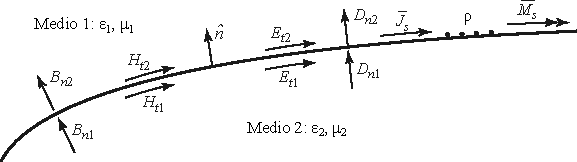
\includegraphics[width=0.8\textwidth]{intro_electro/condiciones_borde.pdf}
	\caption{Corrientes, campos y carga superficial en una interfaz general entre dos medios \cite{Pozar:MwEngineering}.}.
	\label{fig:condiciones_borde}
\end{figure}

Si se considera una interfaz entre dos medios, como la que se muestra en la figura \ref{fig:condiciones_borde}, a partir de las ecuaciones de Maxwell y los teoremas integrales, se pueden deducir las siguientes condiciones de borde:
\begin{subequations}
	\label{eq:condiciones_borde}
	\begin{align}
		\hat{n} \cdot (\vec{D}_{2} - \vec{D}_{1}) & = \rho_s \\
		\hat{n} \cdot (\vec{B}_{2} - \vec{B}_{2}) & = 0 \\
		\hat{n} \times (\vec{E}_2 - \vec{E}_1)  & = - \vec{M}_s \\
		\hat{n} \times (\vec{H}_2 - \vec{H}_1) & = \vec{J}_s
	\end{align}
\end{subequations}

%\paragraph{Campos sobre una superficie dieléctrica}
%Dado que en una interfaz entre dos dieléctricos no hay carga eléctrica ni densidades de corriente, las ecuaciones \ref{eq:condiciones_borde} establecen que las componentes normales de los vectores $\vec{D}$ y $\vec{B}$ se conservan, y que las componentes tangenciales de $\vec{E}$ y $\vec{H}$ también lo hacen.

%\paragraph{Campos sobre una superficie conductora eléctrica}
%Si el conductor no tiene pérdidas ($\sigma \rightarrow \infty$), todos los campos deben ser cero en su interior \footnote{La profundidad de penetración, definida en secciones siguientes, se anula.}. Considerando, además, que $\vec{M}_s = 0$, la componente tangencial del campo eléctrico, $E_t$ desaparece sobre la superficie del conductor. Dado que la diferencia entre las componentes normales del campo magnético está dada por $\vec{J}_s$, y el campo magnético debe anularse en el conductor, la densidad de corriente superficial está dada únicamente por el campo magnético externo al mismo. En el mismo sentido, la densidad de carga superficial $\rho_s$ es la expresión, sobre la superficie del conductor, de la componente normal de $\vec{D}$.

% SKIN DEPTH

%\paragraph{Campos sobre una superficie conductora magnética}
%Dado que la superficie conductora magnética representa el caso dual al de la superficie conductora eléctrica, en este caso se espera que la componente tangencial de $\vec{H}$ se anule sobre la superficie, mientras que la componente tangencial del campo eléctrico dé lugar a corrientes magnéticas sobre la misma.

%%%%% QUEDA DECRI QUE PASA CON UNA CORRIWENTE EN HORIZRAON O VERTICAL - LIBRO DE YAMAT, PAG 10.
%% COMPLETAR CON COLLIN %%

\section{Ecuación de onda}
\label{subsec_eq_de_onda}
%%%%

Al considerar una región del espacio lineal, isotrópica y homogénea, se puede calcular el rotor de la primera ecuación de Maxwell y aplicar la segunda\footnote{Se deberá utilizar la identidad $\nabla \times \nabla \times \vec{E} = \nabla \nabla \cdot \vec{E} - \nabla^2\vec{E}$, donde $\nabla \cdot \vec{E} = \rho/\epsilon$. Aplicando, además, lo mismo para el campo magnético, y considerando que $\nabla \cdot \vec{B} = 0$: \newline % OJO QUE PUEDE ROMPER TODO
	
	
	\begin{tabular}{ r l | r l }
		 $\nabla \times \nabla \times \vec{E}$ & $=\; -j \omega \mu \nabla \times \vec{H} - \nabla \times \vec{M}$ & $\nabla \times \nabla \times \vec{H}$ & $=\; j \omega \nabla \times \vec{D} +  \nabla \times \vec{J}$ \\
		 $\nabla \nabla \cdot \vec{E} - \nabla^2 \vec{E}$ & $=\; -j \omega \mu \nabla \times \vec{H} - \nabla \times \vec{M}$ & $\nabla \nabla \cdot \vec{H} - \nabla^2 \vec{H}$ & $=\; j \omega \epsilon \nabla \times \vec{E} + \nabla \times \vec{J}$ \\
		 $\frac{\nabla \rho}{\epsilon} - \nabla^2 \vec{E}$ & $=\; \omega^2 \mu \epsilon \vec{E} - j \omega \mu \vec{J} - \nabla \times \vec{M}$ & $\frac{1}{\mu} \nabla (\cancelto{0}{\nabla \cdot \vec{B}}) - \nabla^2 \vec{H}$ & $=\; j \omega \epsilon (-j \omega \vec{B} - \vec{M}) + \nabla \times \vec{J}$ \\
		 $\nabla^2 \vec{E} + \omega^2 \mu \epsilon \vec{E}$ & $=\; j \omega \mu \vec{J} + \frac{\nabla \rho}{\epsilon} + \nabla \times \vec{M}$ & $\nabla^2 \vec{H} + \omega^2 \epsilon \mu \vec{H}$ & $=\;  j \omega \epsilon \vec{M} - \nabla \times \vec{J}$
	\end{tabular}	
	}, lo que da como resultado las expresiones \footnote{De estas ecuaciones, se observa que el campo magnético está determinado por la componente rotacional de la corriente eléctrica, mientras que el campo eléctrico está determinado por todas las componentes de la misma. De manera análoga, se cumple la relación inversa para el caso de la corriente magnética.}:

\begin{subequations}
	\begin{align}
		\nabla^2 \vec{E} + \omega^2 \mu \epsilon \vec{E} & = j \omega \mu \vec{J} + \frac{\nabla \rho}{\epsilon} + \nabla \times \vec{M} \label{eq:eq_ondas_completa_E} \\
		\nabla^2 \vec{H} + \omega^2 \epsilon \mu \vec{H} & =  j \omega \epsilon \vec{M} - \nabla \times \vec{J}. \label{eq:eq_ondas_completa_H}
	\end{align}
	\label{eq:eq_ondas_completa_E_H}
\end{subequations}

Si, además, la región del espacio es libre de fuentes ($J=0$, $M=0$ y $\rho=0$), se deducen las ecuaciones de Helmholtz para ambos campos, donde $\gamma$ es el número de onda, en unidades de $(1/m)$:

\begin{equation}
	\label{eq:Helmholtz}
	\begin{aligned}
		\nabla^2  \vec{E} + \gamma^2 \vec{E} &= 0  \\
		\nabla^2 \vec{H} + \gamma^2 \vec{H}& = 0. 
	\end{aligned}
\end{equation}
%%%%

Para el caso sin pérdidas se puede expresar como $\gamma = \beta = \omega \sqrt{\mu \epsilon}$, mientras que si se considera que existen pérdidas óhmicas,  su efecto puede ser tenido en cuenta si  $\gamma$ asume un valor complejo, tal que

\begin{align}
\label{eq:constante-propagacion-compleja}
\gamma = -j\alpha + \beta &= j\omega \sqrt{\mu (\epsilon'-j\epsilon'') - j \sigma \epsilon/\omega}.
\end{align}

Para el caso de un buen conductor, la expresión de $\gamma$ resulta

\begin{align}
\gamma = -j\alpha + \beta &= j \omega \sqrt{\mu \epsilon} \sqrt{\sigma/(\omega \epsilon)} = (1+j) \sqrt{\omega \mu \sigma/2},
\end{align}

lo que nos permite definir la profundidad de penetración como 

\begin{align}
\label{eq:prof_penetacion}
\delta_s = -1/\alpha &= \sqrt{\frac{2}{\omega \mu \sigma}}.
\end{align}

En coordenadas cartesianas, para resolver las ecuaciones \ref{eq:Helmholtz} resulta sencillo aplicar el método de separación de variables\footnote{En coordenadas cartesianas, $\nabla^2 E = \frac{\partial^2 \vec{E}}{\partial x^2} + \frac{\partial^2 \vec{E}}{\partial y^2} + \frac{\partial^2 \vec{E}}{\partial z^2}$. Reemplazando las coordenadas $E_i$ de $\vec{E}, para i=x,y,z$ por funciones $f(x),g(y),h(z)$ independientes entre sí, se obtiene que $\frac{f''(x)}{f(x)} + \frac{g''(y)}{g(y)} + \frac{h''(z)}{h(z)} + \beta_0^2 = 0$. Como las funciones $f$,$g$ y $h$ son independientes, se deduce que $\frac{f''(x)}{f(x)} = -\beta_x^2$, $\frac{g''(y)}{g(y)} = -\beta_y^2$ y $\frac{h''(z)}{h(z)} = -\beta_z^2$.}, que da lugar a ecuaciones cuya solución es de la forma $e^{\pm j \beta_i i}$, con $i = x, y$ o $z$, respectivamente. Las soluciones con un signo positivo en el exponente corresponden a ondas que viajan en la dirección negativa ($-x, -y, -z$), mientras que las que tienen un signo negativo corresponden a ondas que viajan en la dirección positiva. Dado que ambas soluciones son válidas y posibles, en función de las condiciones de borde, en general la expresión de la propagación de los campos electromagnéticos quedará establecida como la suma de ambas, afectadas por un factor de amplitud dependiente de la coordenada evaluada.

Para el caso de ondas que viajan en la dirección positiva,

\begin{equation}
	\label{eq:electric_field_wave_solution}
	\vec{E}(x,y,z) = \vec{E}_0 \;e^{-j(\gamma_x x + \gamma_y y + \gamma_z z)} = \vec{E}_0 \;e^{-j\vec{\gamma}\cdot\vec{r}},
\end{equation}

donde se consideró que $\vec{E}_0 = A \hat{x} + B \hat{y} + C \hat{z}$, $\vec{r} = x \hat{x} + y \hat{y} + z \hat{z}$ y

\begin{equation}
\label{eq:numero_de_onda}
\gamma_x^2 + \gamma_y^2 + \gamma_z^2 = \gamma^2. \\
\end{equation}


Al expresar la divergencia del campo eléctrico de la ecuación \ref{eq:electric_field_wave_solution}, se obtiene\footnote{Aplicando $\nabla \cdot (f \vec{A}) = \vec{A} \cdot \nabla f + f \nabla \cdot \vec{A}$ a la expresión, resulta $\nabla \cdot \vec{E} = \vec{E}_0 \cdot \nabla e^{-j \vec{\beta} \vec{r}} + e^{-j \vec{\beta} \vec{r}}\nabla \cdot \vec{E}_0$, donde $\nabla \cdot \vec{E}_0 =0$}


\begin{align}
\nabla \cdot \vec{E} = \nabla \cdot \vec{E}_0 e^{-j\vec{\gamma} \cdot \vec{r}} & = -j \vec{\gamma} \cdot \vec{E}_0 e^{-j \vec{\gamma} \cdot \vec{r}} = 0,
\end{align}

de lo que se puede deducir que $\vec{\gamma} \cdot \vec{E}_0 = 0$, de modo que el campo eléctrico, en una onda plana, es siempre perpendicular a la dirección de propagación.

De la ecuación de Faraday de \ref{eq:Maxwell}, considerando espacio libre de cargas, se obtiene que, para una onda plana en un medio sin pérdidas, el campo magnético es siempre ortogonal al campo eléctrico y a la dirección de propagación, y que los campos están relacionados de forma que \cite{Fernandez:Electromag}

\begin{align}
	\label{eq:relacion-e-h-ondaplana}
	\vec{H}(\vec{r},t) &= \pm \frac{\hat{\beta} \times \vec{E}(\vec{r},t)}{\eta},
\end{align}

donde $\eta$ es la impedancia de onda, que tiene la forma

\begin{align}
	\eta &= \frac{j \omega \mu}{\gamma }.
\end{align}

Para el caso con pérdidas, y considerando que la dirección de propagación es $z$, las componentes $x$ e $y$ se comportan como

\begin{equation}
E_i(z) = E_i \; e^{-j\gamma z} = E_i \; e^{-\alpha z} \; e^{-j \beta z}, \quad i=x,y. \nonumber
\end{equation}

Si el medio es el vacío, la impedancia intrínseca se denota $\eta_0$ y tiene un valor de $377\; \Omega$, mientras que para otros materiales está determinada por su permitividad eléctrica y permeabilidad magnética, y puede ser compleja si hay pérdidas.

La velocidad de fase se define como $v_p=\omega/\beta$, que de no haber pérdidas queda como $1/\sqrt{\mu \epsilon}$, y que para el caso particular del vacío, se expresa como $1/\sqrt{\mu_0 \epsilon_0} = c$, donde $c$ es la velocidad de la luz en el vacío. Así, la velocidad de fase en cualquier medio material sin pérdidas resulta $c/\sqrt{\epsilon_r \mu_r}$.

La longitud de onda, $\lambda$, es la distancia espacial entre dos máximos sucesivos, por lo que se expresa como $\lambda = 2\pi / \beta = v_p/f$.

\section{Guias de ondas}
\label{subsec_guias_de_ondas}
%%%%
%Pozar, pag 171
%%%%

Suponiendo una guía de ondas de forma arbitraria en la que la energía electromagnética se propaga en la dirección $z$, los campos eléctrico y magnético se pueden expresar como la suma de sus componentes longitudinales (en la dirección $z$) y sus componentes transversales (en el plano $xy$), con constantes $\gamma_z$ y $\gamma_t$, respectivamente, de modo que $\gamma_z + \gamma_t = \gamma$, y dependientes sólo de la posición en el plano transversal, de manera que

\begin{align}
	\vec{E}(x,y,z) = \left[ \vec{e}_{xy}(x,y) + \hat{z} e_z(x,y) \right] e^{-j\gamma z}.
\end{align}

Aplicando las ecuaciones rotacionales de Maxwell (Faraday y Ampère en la ecuación \ref{eq:Maxwell}), considerando una región libre de cargas y un comportamiento armónico de los campos, así como un comportamiento sin pérdidas ($\gamma_z = \beta_z$), se puede deducir que las componentes transversales quedan en términos de las componentes longitudinales \cite{Fernandez:Electromag}

\begin{equation}
	\begin{aligned}
		H_x &= \frac{j}{\gamma_t^2} \left(\omega \epsilon \frac{\partial E_z}{\partial y} - \beta_z \frac{\partial H_z}{\partial x} \right), & H_y &= \frac{-j}{\gamma_t^2} \left(\omega \epsilon \frac{\partial E_z}{\partial x} + \beta_z \frac{\partial H_z}{\partial y} \right),\\
		E_x &= \frac{-j}{\gamma_t^2} \left(\omega \mu \frac{\partial H_z}{\partial y} + \beta_z \frac{\partial H_z}{\partial x} \right), & E_y &= \frac{j}{\gamma_t^2} \left(\omega \mu \frac{\partial H_z}{\partial x} - \beta_z \frac{\partial E_z}{\partial y} \right),
	\end{aligned}
	\label{eq:campos_guia_de_ondas}
\end{equation}

donde se definió $\gamma_t^2 = \gamma^2 - \beta_z^2$ como el número de onda de corte, siendo $\gamma = \omega \sqrt{\mu \epsilon}$, que para el caso sin pérdidas es, además, $\gamma = \beta = 2\pi/\lambda$, el número de onda  en el material que rellena la línea de transmisión.

Cuando no existen componentes de campo en la dirección de propagación, $z$, según las ecuaciones \ref{eq:campos_guia_de_ondas}, no existen campos en las direcciones transversales si $\gamma_t \neq 0$. La indeterminación generada por el hecho de que $\gamma_t$ se anula da como resultado que $\beta_z = \omega \sqrt{\mu \epsilon} = \beta$, de modo que no existe número de onda de corte, y haciendo que la impedancia de onda sea $\eta$.  A este modo de propagación sobre una guía de ondas se lo llama TEM (transversal electromagnético). Los campos transversales satisfacen que el Laplaciano es 0, de modo que se comportan como un campo electrostático, y este es el motivo por el cual no pueden existir ondas TEM en guías de ondas de un único conductor.

Cuando la componente $z$ del campo eléctrico se anula, el modo de propagación se denomina TE (transversal eléctrico), y pueden utilizarse las relaciones descriptas en la ecuación \ref{eq:campos_guia_de_ondas} para obtener el resto de los campos. La impedancia de onda, en este caso, resulta $Z_{TE} = \gamma\eta/\beta_z$, dependiente de la frecuencia.

Cuando la componente $z$ del campo magnético se anula, el modo de propagación es TM (transversal magnético), y con el mismo procedimiento que antes, se puede hallar su impedancia de onda, que resulta $Z_{TM} = \beta_z \eta / \gamma$.

\section{Ondas de superficie}
\label{sec:ondas-de-superficie}
Existen estructuras abiertas que son capaces de mantener el campo electromagnético íntimamente ligadas a ellas, de forma que el mismo decaiga exponencialmente con la distancia a las mismas (comportamiento evanescente), y simultáneamente permiten propagación de energía en una dirección $z$ paralela a la superficie (con un decrecimiento inverso a la raíz cuadrada de la distancia, debido a la expansión del frente de onda), dando lugar a lo que se conoce como ondas de superficie \cite{Barlow:SurfaceWaves}. Estas estructuras se denominan guías de ondas superficiales, y pueden consistir en planos conductores recubiertos de dieléctrico, en planos corrugados o en simples interfaces entre dos medios distintos. Uller inauguró el campo en 1903, y luego Zenneck y Sommerfeld, entre 1907 y 1909, las utilizaron para explicar la propagación de ondas en la superficie terrestre, aunque este último utilizó la expresión ``ondas de superficie" para referirse al efecto conjunto de ondas espaciales y ondas de superficie \cite{Barlow:SurfaceWaves}, que no se corresponde completamente con la definición actual. Recién en la década de 1950 se realizaron estudios teóricos de importancia, que permitieron hallar aplicaciones y nuevas estructuras que permiten la propagación de este tipo de ondas.

En la actualidad, las ondas de superficie se clasifican en ondas Zenneck (utilizadas en bajas frecuencias, cuando los medios intervinientes poseen altas pérdidas), ondas de tipo resonante (que surgen cuando una onda plana incide sobre un material periódico), ondas de superficie no lineales (que se generan en medios no lineales), plasmones (utilizados en altas frecuencias, cuando los medios tienen bajas pérdidas) y ondas de Dyakonov (donde al menos uno de los materiales es anisotrópico), entre otras.

Para este trabajo, resultan de importancia las ondas de Zenneck, ya que permiten explicar el comportamiento de las ondas sobre una placa dieléctrica fina que posee un plano conductor en una de sus caras. Una representación tridimensional de las mismas se puede observar en la figura \ref{fig:onda-superficie-3d}.

\begin{figure}[htp]
	\centering
	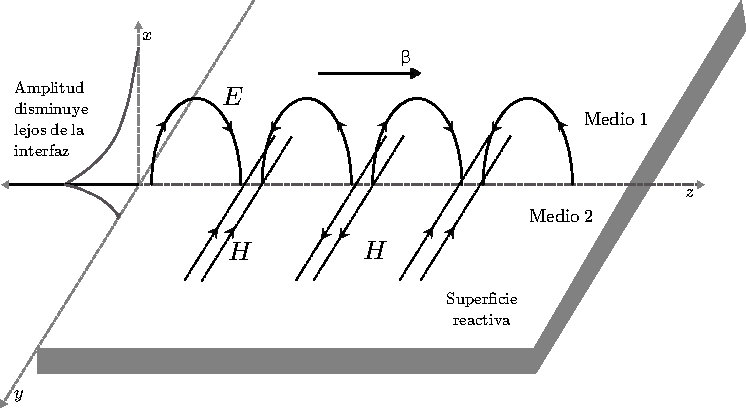
\includegraphics[width=0.8\textwidth]{intro_electro/ondas-superficie-3d.pdf}
	%\input{Figures/intro_electro/onda-superficie-incidencia-brewster3.pdf_tex}
	\caption{Representación gráfica del comportamiento de una onda de superficie TM sobre una interfaz reactiva.}
	\label{fig:onda-superficie-3d}
\end{figure}

Si se considera que una onda plana incide con ángulo de Brewster (concepto desarrollado en el anexo \ref{sec:incidencia-onda-plana-interfaz}) en modo TM sobre una interfaz entre dos medios de bajas pérdidas ($\epsilon'' \ll \epsilon'$), cada uno con una permitividad eléctrica $\epsilon_i$ y una permeabilidad magnética $\mu_i$, $i=1,2$, como indica la figura \ref{fig:onda-superficie-brewster}, no existirá energía reflejada. De esta forma, toda la energía incidente es entregada a la interfaz, y se obtienen las expresiones \ref{eq:ondas-superficie-campos}, donde no existen componentes reflejadas y donde T es el factor de transmisión. Con el fin de simplificar dichas ecuaciones, se considera que el medio 1 es aire, de modo que $\epsilon_1 = \epsilon_0$, $\mu_1 = \mu_0$ y, en consecuencia, $\eta_1 = \eta_0$.

\begin{figure}[htp]
	\centering
	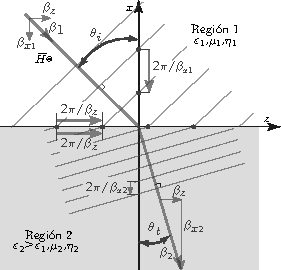
\includegraphics[width=0.7\textwidth]{intro_electro/onda-superficie-incidencia-brewster.pdf}
	%\input{Figures/intro_electro/onda-superficie-incidencia-brewster3.pdf_tex}
	\caption{Ilustración del comportamiento de una onda plana durante la incidencia TM con ángulo de Brewster. Las rectas paralelas representan los frentes de onda, es decir, son rectas de fase constante. Es importante destacar que la longitud de onda paralela a la interfaz, $2\pi/\beta_z$, se mantiene constante a ambos lados, dado que sobre la interfaz se intersecan las rectas de fase constante.}
	\label{fig:onda-superficie-brewster}
\end{figure}

\begin{subequations}
	\label{eq:ondas-superficie-campos}
	\begin{align}
	{H_1}_y &= A e^{-j\ (z\; \overbrace{\gamma_1\;\sin \theta_i}^{\gamma_z} - x\; \overbrace{\gamma_1\;\cos \theta_i}^{\gamma_{x_1}})},\;\; x>0 & j\omega\epsilon E_x &= -\frac{\partial H_y}{\partial z}, \\
	{H_2}_y &= A T e^{-j\; (z\; \overbrace{\gamma_2\; \sin \theta_t}^{\gamma_z} - x\; \overbrace{\gamma_2\; \cos \theta_t}^{\gamma_{x_2}})},\;\; x<0   & j\omega\epsilon E_z &= -\frac{\partial H_y}{\partial x} .
	\end{align}
\end{subequations}

La componente longitudinal de los vectores de onda, $\gamma_z$, es igual a ambos lados de la interfaz, como se muestra en la figura \ref{fig:onda-superficie-brewster} (en términos de $\beta_z$, ya que no se consideran pérdidas), de modo que

\begin{equation}
	\gamma_{1} \; \sin \; \theta_t = \gamma_{z} = \gamma_2 \; \sin \; \theta_i.
\end{equation}

Las componentes normales a la interfaz, que llamaremos $\gamma_{x_i}$, $i=1,2$, mostradas también en la figura \ref{fig:onda-superficie-brewster}, deben cumplir que

\begin{align}
	\label{eq:condicion-componentes-normales-ondas-superficie}
	& \gamma_{x_1}^2 + \gamma_z^2 = \gamma_1^2 &\text{y} &&\gamma_{x_2}^2 + \gamma_z^2 = \gamma_2^2.
\end{align}

Las impedancias de onda en ambas regiones se obtienen como la relación entre los campos tangenciales a la interfaz sobre la que se incide, de modo que

\begin{subequations}
\label{eq:impedancia-onda-superficie}
\begin{align}
	Z_1 = \frac{{E_z}_1}{{H_y}_1} = \eta_0 \; \cos\; \theta_i &\implies Z_1 = \frac{\gamma_{x_1}}{\gamma_1} \eta_0, \label{eq:impedancia-onda-incidente-onda-sup}\\
	Z_2 = \frac{{E_z}_2}{{H_y}_2} = \eta \; \cos \; \theta_t &\implies Z_2 = \frac{\gamma_{x_2}}{\gamma_2} \eta. \label{eq:impedancia-onda-transmitida-onda-sup}
\end{align}
\end{subequations}

Para poder considerar que toda la energía de la onda incidente se transmite desde el primer medio al segundo, debe suceder que las impedancias de onda a ambos lados de la interfaz sean iguales ($Z_1 = Z_2$). Igualando las ecuaciones \ref{eq:impedancia-onda-incidente-onda-sup} y \ref{eq:impedancia-onda-transmitida-onda-sup}, se deduce\footnote{Al igualar las expresiones de las impedancias de onda, se obtiene $\frac{\gamma_{x_1} \eta_0}{\gamma_1} = \frac{\gamma_{x_2} \eta_2}{\gamma_2}$. Recordando que $\gamma_1=\omega \sqrt{\mu_0 \epsilon_0}$, $\gamma_2=\omega \sqrt{\mu_0 (\epsilon'-j\epsilon'')}$, $\eta_0 = \sqrt{\mu_0 / \epsilon_0}$ y $\eta = \sqrt{\mu_0 / (\epsilon'-j\epsilon'')}$, se deduce que la relación entre $\gamma_{x_1}$ y $\gamma_{x_2}$ es compleja: $\gamma_{x_1}\; (\epsilon' - j \epsilon'') = \gamma_{x_2} \epsilon_0$, de modo que en forma general se puede considerar que tanto $\gamma_{x_1}$ como $\gamma_{x_2}$ son complejos.} que, en forma general, si el medio sobre el que se incide tiene pérdidas, entonces $\gamma_{x_1}$ y $\gamma_{x_2}$ son complejos. De esta manera, $\gamma_{x_1} = \beta_{x_1} - j\alpha_{x_1}$ y $\gamma_{x_2} = \beta_{x_2} - j\alpha_{x_2}$, lo que significa que además de avanzar en fase, la onda pierde energía, pues tiene un comportamiento evanescente, de modo que el vector de Poynting tiene una componente en la dirección perpendicular a la interfaz, que se atribuye al consumo de energía de la misma \cite{Barlow:SurfaceWaves}. Dado que $\vec{\gamma_1} = \vec{\gamma_{z_1}} + \vec{\gamma_{x_1}}$, resulta conveniente considerar que la constante de propagación, $\gamma_{z_1} = \beta_{z_1} - j \alpha_{z_1}$, posee también un valor complejo.

El campo magnético queda, entonces, expresado como:

\begin{equation}
	H_y =
	\left\lbrace
	\begin{aligned}
		A e^{-j\beta_z z -\alpha_{z_1} z + j\beta_{x_1}x - \alpha_{x_1}x}, \quad x>0, \\
		A e^{-j\beta_z z -\alpha_{z_2} z + j\beta_{x_1}x + \alpha_{x_2}x}, \quad x<0. \\
	\end{aligned}
	\right.
\end{equation}

Se observa que los planos de fase constante, en el aire, son los correspondientes a las exponenciales imaginarias de la ecuación anterior, $\beta_z z - \beta_{x_1}x = cte$, y se muestran en la figura \ref{fig:onda-superficie-brewster}. Los planos de amplitud constante se obtienen considerando las exponenciales decrecientes de las expresiones, de forma que $\alpha_{z_1}z + \alpha_{x_1}x = cte$, que para el caso analizado en la figura \ref{fig:onda-superficie-brewster}, son rectas con pendiente negativa (no mostradas en la figura). Esto es así porque en la expresión se considera que existen pérdidas en la dirección $z$ paralela a la interfaz. De no haber pérdidas, los planos de amplitud constante resultan paralelos a la misma.

Para bajas pérdidas, $\alpha_{z_i}$, $i=1,2$, será pequeño, por lo que habrá baja atenuación para la onda que se desplaza en dirección $z$, pero debido a que $\alpha_{x_1}$ y/o $\alpha_{x_2}$ también serán bajas, la energía no estará concentrada cerca de la interfaz.



Si se considera una superficie con una impedancia de onda para polarización TM normalizada respecto de $\eta_0$, $Z_s = R_s + j X_s$, independiente del ángulo de incidencia, entonces, al igualar la impedancia de onda a la impedancia de superficie, y teniendo en cuenta las igualdades de la ecuación \ref{eq:impedancia-onda-superficie}, resulta, en el caso TM,

\begin{align}
	\gamma_{x_1} & = \gamma_1 \frac{Z_1}{\eta_0} = \gamma_1 Z_s = \gamma_1 R_s + j \gamma_1 X_s, \label{eq:h1-onda-superficie}\\
	\gamma_z &= \beta_z - j\alpha_z =\sqrt{(\gamma_1^2 - \gamma_{x_1}^2)} = \gamma_1 \sqrt{1+X_s^2 - R_s^2 - 2jR_s X_s}. \label{eq:beta-onda-superficie}
\end{align}

La gráfica de las componentes real e imaginaria de $\gamma_z$ se muestra en la figura \ref{fig:beta-reactancia-TM}. Se puede observar que, cuando la reactancia es inductiva (valores positivos de $X_s$), $\alpha_z$ presenta valores positivos, por lo que habrá atenuación en la dirección de propagación $z$ ([a] en la figura) \footnote{Esto se debe a que si el campo eléctrico en la dirección $y$ se escribe como se indica en la ecuación \ref{eq:ondas-superficie-campos}, $\gamma_z=\beta_z-j\alpha_{z_i}, i=1,2$ y $\gamma_{x_1} = \beta{x_1}+j\alpha_{x_1}$, el exponente se expresa como $-j(\beta_z-j\alpha_{z_1})z + j(\beta_{x_1}+j\alpha_{x_1})x$. Para dirección de propagación $z$, con $z>0$, la componente de atenuación del exponente de la expresión dada resulta en $-\alpha_{z_i} z, i=1,2$. Para que el comportamiento resulte decreciente, $\alpha_{z_i}$ debe ser mayor a $0$.}. Esto significa que, a mayor reactancia, habrá una mayor disminución de la amplitud del campo a medida que la onda se desplace por la interfaz (aumenta el valor de $z$). Sin embargo, la mayor variación en el coeficiente de atenuación se observa con el cambio de valor de la resistencia, $R_s$ ([b] en la figura).

Si la reactancia es nula, un valor de $\beta_z$ se obtiene sólo si la resistencia es muy baja o nula ([c] en la figura). Esto significa que sobre una superficie puramente resistiva, sólo habrá propagación de ondas de superficie cuando la resistencia sea inferior a un umbral dependiende de los medios materiales ($\beta_z=0$, [d] en la figura). Cuando ese umbral de resistencia es superado, el valor de la constante de propagación paralela a la interfaz se anula.

El comportamiento de $\gamma_{x_1}$ (la componente ortogonal a la superficie), descripto en la ecuación \ref{eq:h1-onda-superficie} también regula el comportamiento de la onda de superficie, dado que si la magnitud de la parte imaginaria de $\gamma_{x_1}$, $\alpha_{x_1}$, es muy pequeña, la onda no estará lo suficientemente cerca de la interfaz para ser guiada por ella. Un valor alto de $\alpha_{x_1}$ se da cuando la reactancia, $X_s$ es inductiva ($X_s>0$), lo cual coincide con el requisito para $\alpha_{z_i}, i=1,2$. Dicho de otra forma, la reactancia de superficie es la responsable del decrecimiento exponencial de la onda al aumentar la distancia con la interfaz que funciona como guía.

Analizando la ecuación \ref{eq:beta-onda-superficie}, se deduce que un producto $R_s X_s$ pequeño dará lugar a atenuaciones pequeñas en la onda de superficie, de modo que para que se propague una onda sobre la interfaz, si se establece $X_s$ grande para obtener un valor de $\beta_z$ grande, se deben disminuir el comportamiento resistivo tanto como sea posible ([e] en la figura).

\begin{figure}[htp]
	\centering
	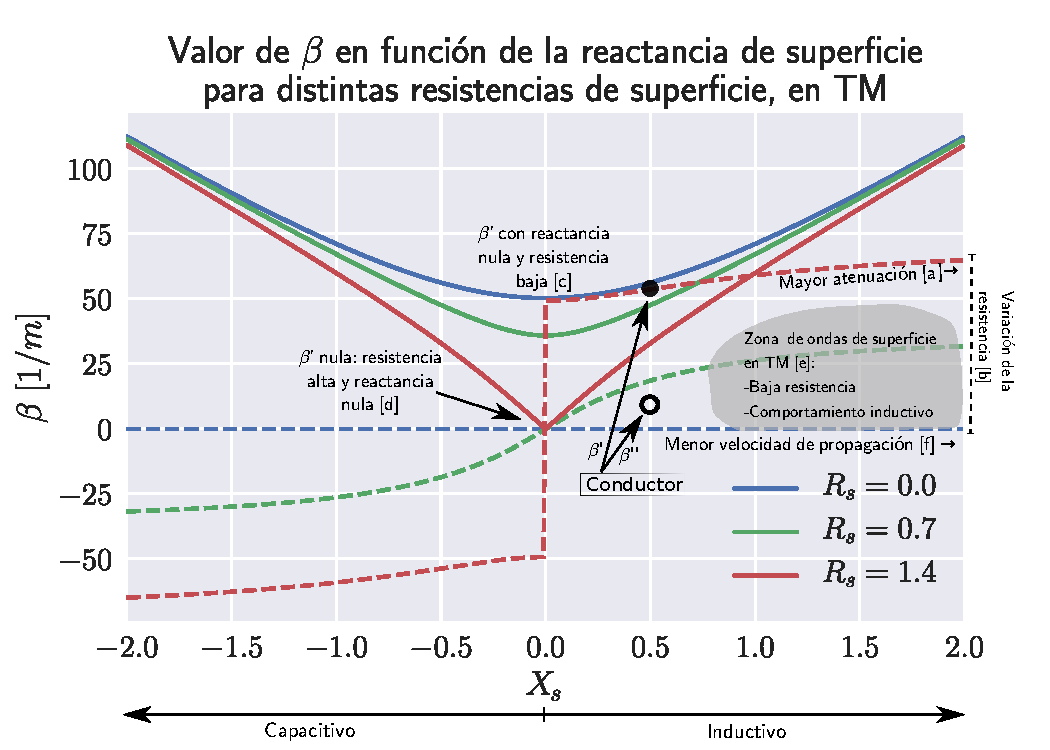
\includegraphics[width=\textwidth]{intro_electro/plot-beta-reactancia-TM.pdf}
	%\input{Figures/intro_electro/onda-superficie-incidencia-brewster3.pdf_tex}
	\caption{Comportamiento de la constante de propagación superficial $\gamma_z$ en función de la resistencia y reactancia superficial para el caso de incidencia TM. Las líneas punteadas representan la parte imaginaria de $\gamma_z$, y las líneas completas representan la parte real, de forma que $\gamma_z = \beta_z - j\alpha_z$.}
	\label{fig:beta-reactancia-TM}
\end{figure}

La velocidad de propagación se obtiene directamente de la componente real de $\gamma_z$ que, si $R_s$ es pequeño y $X_s$ es grande, resulta, a partir de la expresión \ref{eq:beta-onda-superficie}, $\beta_z \approx \beta_1 \sqrt{1+X_s^2}$, de forma que la velocidad de fase es

\begin{align}
	v_p = \frac{\omega}{\beta_z} = \frac{c}{\sqrt{1+X_s^2}}.
\end{align}

En los casos en que la componente reactiva de la impedancia de superficie es grande, el valor de la velocidad de propagación es menor al de la luz (denotado como [f] en la figura).

%%%%%%%%%%%%%%%%%

Cuando la interfaz es de tipo aire-conductor, la componente inductiva de la impedancia de superficie (relacionada a la profundidad de penetración) resulta igual a la componente resistiva, de forma que \cite{Fernandez:Electromag}

\begin{align}
	\eta &= \frac{1+j}{\sigma \delta}.
\end{align}
 
Aplicando las ecuaciones \ref{eq:beta-onda-superficie}, se obtiene que\footnote{Considerando que $\gamma=\omega\sqrt{\epsilon \mu}$, $\eta_0=\sqrt{\epsilon_0}/\sqrt{\mu_0}$ y que $\delta=\sqrt{\frac{2}{\omega \mu_0 \sigma}}$, se observa que $\gamma/\eta_0=\frac{\omega \sqrt{\epsilon_0 \mu_0}}{\frac{\sqrt{\epsilon_0}}{\mu_0}}=\omega \mu_0$, por lo que se puede expresar a $\delta$ como $\frac{2 \eta_0}{\gamma \sigma}$.}

\begin{align}
	\gamma_x &= \gamma_1 (1+j) \sqrt{\frac{\gamma_1}{2 \sigma Z_0}}, \\
	\gamma_z &= \gamma_1 \sqrt{1-\frac{j \gamma_1}{\sigma Z_0}} \approx \gamma_1 - \frac{j  \gamma_1^2}{2 \sigma Z_0}.
\end{align}

En general, un plano conductor soporta ondas de superficie, y la atenuación en la dirección de propagación es muy baja (ver figura \ref{fig:beta-reactancia-TM}), pero no es capaz de lograr una atenuación en la dirección normal al mismo tal que la energía se mantenga concentrada en la superficie para poder ser utilizada como guía de ondas, debido a que la conductividad es muy alta (lo que disminuye el valor de ${\alpha_x}_1$). Para lograr que la energía de la onda decaiga rápidamente lejos de la interfaz es necesario aumentar notoriamente la reactancia de la superficie, para lo que se suele agregar al conductor una capa dieléctrica, que además no aumenta considerablemente la resistividad.

Para el caso de ondas de superficie en modo TE, los campos están dados por la ecuación \ref{eq:campo-electrico-superficie-TE}. La impedancia de onda, en tanto, queda expresada como indica la ecuación \ref{eq:impedancia-onda-superficie-TE}. Considerando que, para evitar reflexiones, la impedancia de superficie tiene que ser igual a la impedancia de onda, se obtiene la expresión para la constante de propagación en el sentido perpendicular a la interfaz mostrada en la ecuación \ref{eq:h1-onda-superficie-TE}, donde nuevamente la impedancia de superficie del conductor es $Z_s = R_s +jX_s$.

\begin{equation}
	\label{eq:campo-electrico-superficie-TE}
	\begin{aligned}
		E_y = A e^{j\gamma_x x-j\gamma_z z}, \qquad j\omega \mu_0 H_z = -\frac{\partial E_y}{\partial x}, \qquad j\omega \mu_0 H_x = \frac{\partial E_y}{\partial z}.
	\end{aligned}
\end{equation}

\begin{align}
	\label{eq:impedancia-onda-superficie-TE}
	Z_1 = \frac{E_y}{H_z} = -\frac{\omega \mu_0}{\gamma_{x_1}} = -\frac{\eta \gamma_1}{\gamma_{x_1}}.
\end{align}

\begin{align}
	\label{eq:h1-onda-superficie-TE}
	\gamma_{x_1} = -\frac{\gamma_1}{Z_s} = -\gamma_1 \frac{R_s}{{R_s^2 + X_s^2}}-j\frac{X_s}{R_s^2 + X_s^2}.
\end{align}

Se observa que para que el valor de $\alpha_{x_1}$ resulte positivo, de manera que se de un decrecimiento exponencial desde la superficie, el valor de $X_s$ tiene que ser negativo, por lo que el comportamiento de la superficie tiene que ser capacitivo.

La segunda condición para la existencia de ondas de superficie, la propagación de los campos, está asegurada si $\gamma_z$ es positivo, y si la atenuación en la dirección de propagación, parametrizada por $\alpha_z$, es baja. La expresión de $\gamma_z$ para el caso TE resulta, a partir de \ref{eq:h1-onda-superficie-TE},

\begin{align}
	\gamma_z = \beta_z-j\alpha_z= \sqrt{(\gamma_1^2 - \gamma_{x_1}^2)} = \frac{\gamma_1}{R_s^2+X_s^2} \sqrt{1+X_s^2 - R_s^2 + 2jR_s X_s}. \label{eq:beta-onda-superficie-TE}
\end{align}

Gráficas de la expresión anterior se muestran en la figura \ref{fig:beta-reactancia-TE}, donde se pueden observar valores de $\beta_z$ y $\alpha_{z_1}$ en función de la reactancia $X_s$, para algunos valores de resistencia de superficie $R_s$. Resulta importante destacar que para valores en que $X_s$ es negativa (reactancia capacitiva), el valor de $\alpha_z$ es físicamente realizable, ya que da lugar a un decrecimiento exponencial, y no a un incremento. Por otro lado, al contrario que en el caso de las ondas TM, a medida que la reactancia capacitiva aumenta en módulo, la constante de propagación tiende a estabilizarse en lugar de crecer linealmente, aunque sí decrece la constante de atenuación $\alpha_z$. Cuando la resistencia de superficie es muy baja, los valores de $\beta_z$ para reactancia $X_s$ nula tienden a ser muy altos. Cuando los valores de resistencia aumentan ligeramente, al igual que en el caso TM, el valor de $\beta_z$ se vuelve nulo, lo que obliga a presentar un comportamiento capacitivo para la propagación de ondas de superficie en modo TE.


\begin{figure}[htp]
	\centering
	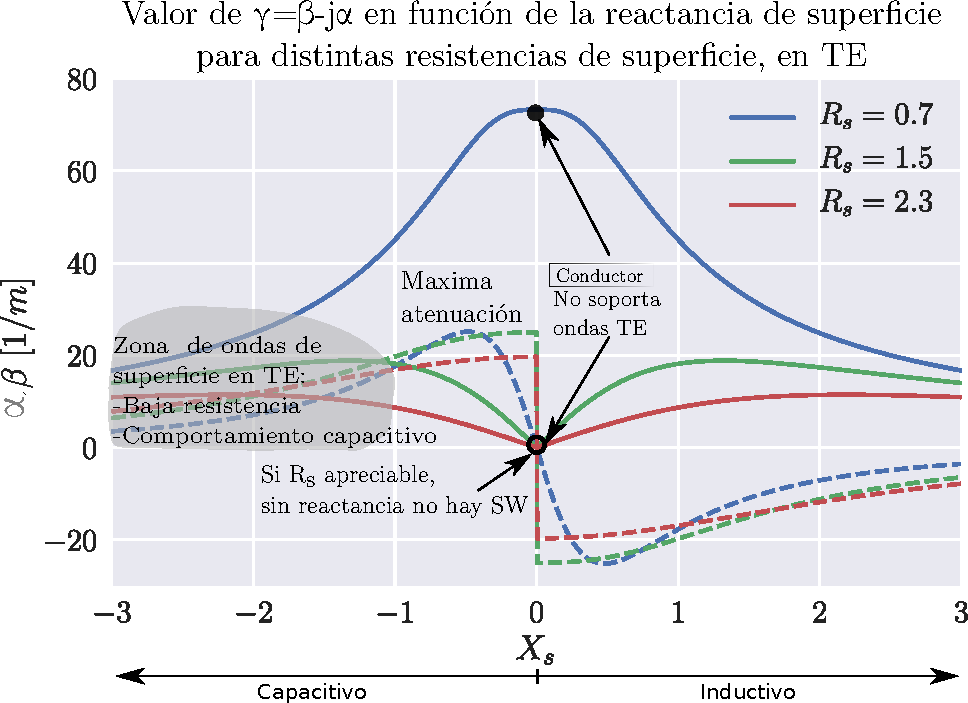
\includegraphics[width=\textwidth]{intro_electro/plot-beta-reactancia-TE.pdf}
	%\input{Figures/intro_electro/onda-superficie-incidencia-brewster3.pdf_tex}
	\caption{Comportamiento de la constante de propagación superficial $\gamma_z$ en función de la resistencia y reactancia superficial para el caso de incidencia TE. Las líneas punteadas representan la parte imaginaria de $\gamma_z$, y las líneas completas representan la parte real, de forma que $\gamma_z = \beta_z - j\alpha_z$.}
	\label{fig:beta-reactancia-TE}
\end{figure}

Entre las distintas formas de lograr que una interfaz conductor-aire permita el guiado de ondas de superficie, una de las más efectivas consiste en el recubrimiento de la superficie metálica por una capa dieléctrica fina, como se muestra en la figura \ref{fig:thin-dielectric-coating}.

\begin{figure}[htp]
	\centering
	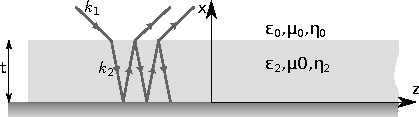
\includegraphics[width=0.7\textwidth]{intro_electro/incidencia-coated-conductor.pdf}
	\caption{Incidencia sobre un conductor recubierto por un dieléctrico.}
	\label{fig:thin-dielectric-coating}
\end{figure}

Para el caso TM, si se considera que el campo magnético tiene la forma de la ecuación \ref{eq:campo-magnetico-TM} en el espacio libre circundante a la estructura, entonces el campo magnético en el interior del dieléctrico resultará de la forma expresada en la ecuación \ref{eq:campo-magnetico-interior-diel-TM}, donde se cumple que $\gamma_{x_1}^2 + \gamma_z^2 = \gamma_1^2$ y $\gamma_{x_2}^2 + \gamma_z^2 = \gamma_2^2 = \epsilon_r \gamma_1^2$.

\begin{align}
	\label{eq:campo-magnetico-TM}
	H_{1_y} = A e^{j\gamma_{x_1} x - j \gamma_z z},\quad x>t.
\end{align}

\begin{align}
	\label{eq:campo-magnetico-interior-diel-TM}
	H_{2_y} = [B e^{j\gamma_{x_2} x} + C e^{-j\gamma_{x_2} x}] e^{-j\gamma_z z},\quad  0\leq x \leq t.
\end{align}

Dado que en toda interfaz las componentes tangenciales de los campos se conservan, y a que las componentes tangenciales del campo eléctrico sobre el conductor se anulan, se deduce que $H_{2_y}$ es un coseno, y se obtienen\footnote{De la ecuación \ref{eq:campo-magnetico-TM} se deriva el campo eléctrico, utilizando la ecuación de Ampère. Al establecer la condición que indica que sobre la interfaz con el conductor no existe campo eléctrico paralelo a la superficie del mismo (se asume un conductor perfecto), se concluye que el valor de B y de C en la ecuación \ref{eq:campo-magnetico-interior-diel-TM} coinciden. Aplicando la condición de continuidad de las componentes tangenciales de los campos sobre la interfaz aire-dieléctrico, se obtiene una relación entre los valores de A y B. Queda expresado el siguiente sistema de ecuaciones:
\begin{equation*}
	\begin{bmatrix}
		-j \gamma_{x_1} e^{-j \gamma_{x_1} t} & -2 \gamma_{x_2}/\epsilon_{r_2} \sin(\gamma_{x_2} t) &  \\
		 -e^{-j \gamma_{x_1} t} & 2 \cos (\gamma_{x_2} t)
	\end{bmatrix}
	\begin{bmatrix}
		A \\
		B
	\end{bmatrix}
	=
	\begin{bmatrix}
		0 \\
		0
	\end{bmatrix}
\end{equation*}

Para que la solución no sea trivial, el determinante de la matriz del sistema tiene que ser nula, lo que da como resultado $\gamma_{x_2} \tan (\gamma_{x_2} t) = -j \gamma_{x_1} \epsilon_{r_2}$.
} las expresiones \ref{eq:solucion-ondas-sup-tm-tan} y \ref{eq:solucion-ondas-sup-tm-h}.


\begin{align}
	\label{eq:solucion-ondas-sup-tm-tan}
	\gamma_{x_2} \tan (\gamma_{x_2} t) = -j \gamma_{x_1} \epsilon_{r_2}, \\
	\gamma_1^2 (\epsilon_{r_2}-1) = \gamma_{x_2}^2 - \gamma_{x_1}^2.
	\label{eq:solucion-ondas-sup-tm-h}
\end{align}

Considerando que $\gamma_{x_1}$ es puramente imaginario positivo\footnote{Un análisis general requiere considerar $\gamma_{x_1}$, $\gamma_{x_2}$ y $\epsilon_2$ como complejos, de manera que se puedan tener en cuenta las pérdidas. Para simplificar el desarrollo, se puede asumir que, dado que se trata de ondas de superficie, la parte imaginaria de $\gamma_{x_1}$ deberá ser negativa, de manera que a mayor distancia de la interfaz, la intensidad de los campos decrezca exponencialmente. La parte real de $\gamma_{x_1}$, si bien puede existir, a efectos del estudio del comportamiento de la onda de superficie en la dirección de propagación, puede obviarse. Por otro lado, si se considera que el ancho del dieléctrico, $t$, es muy pequeño, de forma que se pueda considerar que $\tan(\gamma_{x_2} t) \approx \gamma_{x_2} t$, entonces la expresión \ref{eq:solucion-ondas-sup-tm-tan} resulta aproximadamente $\gamma_{x_2}^2 t = -j \gamma_{x_1} \epsilon_{r_2}$. Asumiendo, por lo explicado antes, que $\gamma_{x_1}$ es valor puramente imaginario positivo, el valor de $\gamma_{x_2}$, obtenido de $\gamma_{x_2}^2 t = \gamma_{x_1} \epsilon_{r_2}$, deberá ser real. Al argumento no descarta la existencia de valores complejos de $\gamma_{x_1}$ y $\gamma_{x_2}$, sino que permite una validación intuitiva del desarrollo posterior.}, la ecuación \ref{eq:solucion-ondas-sup-tm-h} se puede expresar como $\gamma_1^2 (\epsilon_{r_2}-1) = \gamma_{x_2}^2 + |\alpha_{x_1}|^2$. Si se multiplica esta nueva expresión por $t^2$ y a la expresión \ref{eq:solucion-ondas-sup-tm-tan} por $t$, se obtienen dos expresiones que dan lugar a un sistema de ecuaciones trascendentales que se pueden resolver gráficamente, dado que representan una esfera de radio $\gamma_1 t \sqrt{\epsilon_{r_2}-1}$ y una tangente:

\begin{equation}
	\label{eq:sistema-ondas-superficiales-TM}
	\begin{cases}
		(\gamma_{x_2} t)^2 + (\alpha_{x_1} t)^2 = (\epsilon_{r_2} - 1) (\gamma_1 t)^2\\
		\gamma_{x_2} t \tan (\gamma_{x_2} t) = |\alpha_{x_1}| \epsilon_{r_2} t.
	\end{cases}
\end{equation}

Para el caso TE, la solución es similar, y en este caso las expresiones resultan (considerando, nuevamente, que $\gamma_{x_1}$ es puramente imaginario positivo, es decir, $\gamma_{x_1} = \alpha_{x_1}$):

\begin{equation}
	\label{eq:sistema-ondas-superficiales-TE}
	\begin{cases}
		(\gamma_{x_2} t)^2 + (\alpha_{x_1} t)^2 = (\epsilon_{r_2} - 1) (\gamma_1 t)^2 \\
		\gamma_{x_2} t \cot (\gamma_{x_2} t) = -|\alpha_{x_1}| \epsilon_{r_2} t.
	\end{cases}
\end{equation}

Las soluciones se pueden obtener gráficamente para ambos casos, mediante la intersección de las curvas correspondientes a las ecuaciones del sistema. Las gráficas, para distintas frecuencias, se muestran en la figura \ref{fig:intersecciones-tm-te}. Se puede observar que, dado que $|\alpha_{x_1}|t$ no puede tomar valores negativos, las intersecciones que se dan en esas condiciones no son válidas como soluciones del sistema planteado, bajo las hipótesis consideradas.

A medida que aumenta la frecuencia, el valor del radio de los círculos aumenta. Se observa que siempre existe, al menos, un modo TM de propagación sobre el plano de tierra, dado que todas las intersecciones entre las curvas ocurren para valores de $|\alpha_{x_1}| t$ mayores a 0, como se muestra en la figura \ref{fig:soluciones-TM-tan-implicita-zoom}. Para frecuencias en que el radio del círculo genera que el mismo intersecte a más secciones de la curva tangente, aparecerían modos de propagación superiores.

Para el caso TE, se observa que para frecuencias bajas no existe solución válida, como se muestra en la figura \ref{fig:soluciones-TE-tan-implicita-zoom}, por lo que no hay un modo fundamental TE por debajo de la frecuencia de corte, que se da para $f_c = c/(4 t  \sqrt{\epsilon_{r_2}}-1)$, que en el caso graficado es de aproximadamente 25 GHz.

Para el caso de FR4, en el rango de frecuencias de interés para este trabajo, no existe, entonces, propagación de ondas de superficie de polarización TE, por lo que el análisis del modo TM reviste mayor importancia.


\begin{figure} [H]
	\centering 
	\subfigure[TM]{
		\label{fig:soluciones-TM-tan-implicita}
		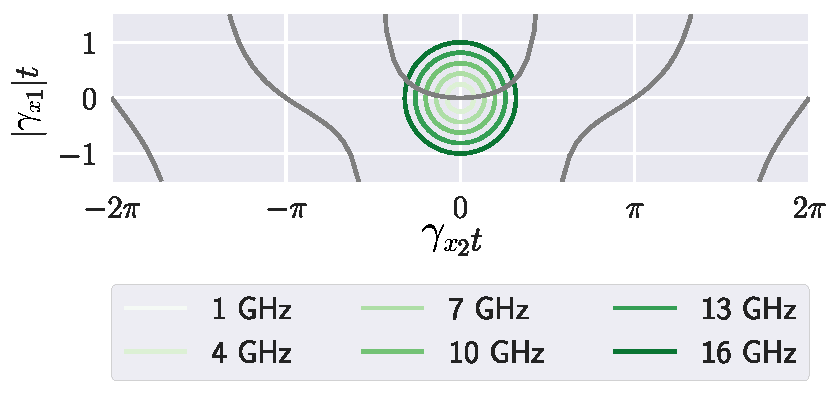
\includegraphics[width=0.48\textwidth]{intro_electro/TM-tan-implicito}}
	\subfigure[TE]{
		\label{fig:soluciones-TE-tan-implicita}
		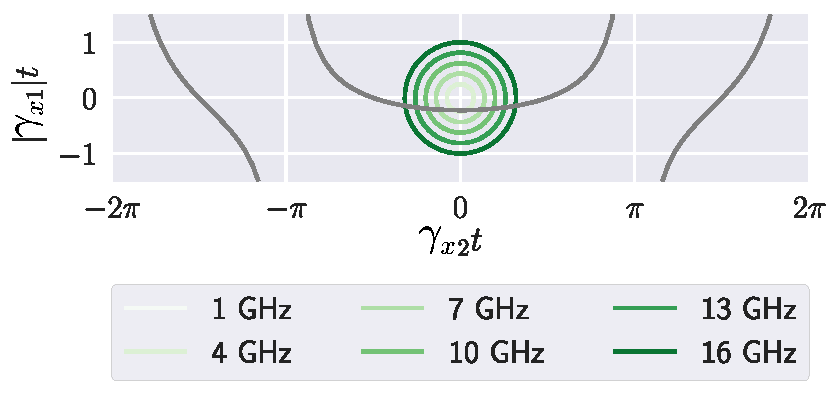
\includegraphics[width=0.48\textwidth]{intro_electro/TE-tan-implicito}}
	\subfigure[Zoom para modo TM]{
		\label{fig:soluciones-TM-tan-implicita-zoom}
		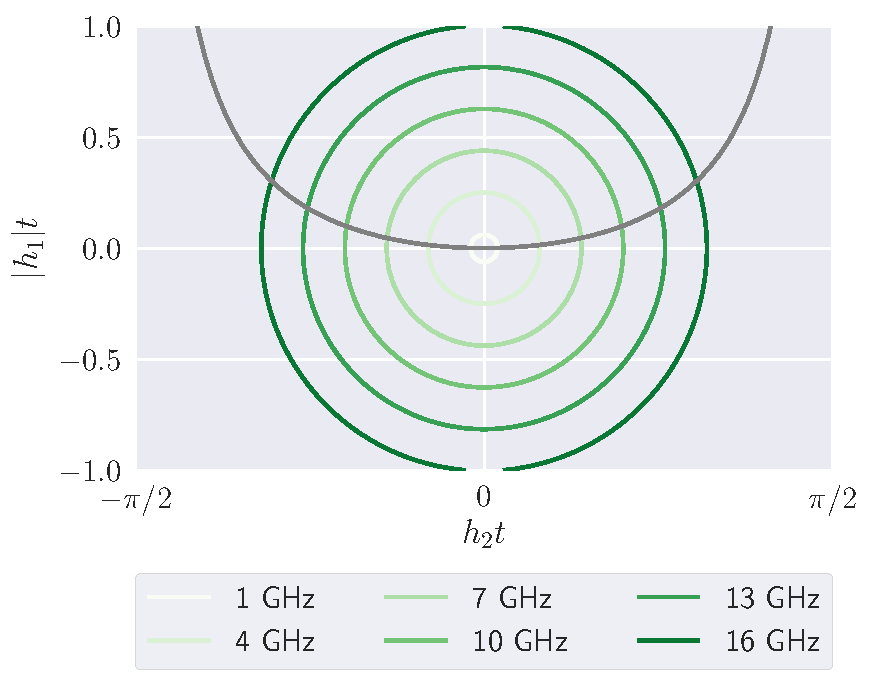
\includegraphics[width=0.48\textwidth]{intro_electro/TM-tan-implicito-zoom}}
	\subfigure[Zoom para modo TE]{
		\label{fig:soluciones-TE-tan-implicita-zoom}
		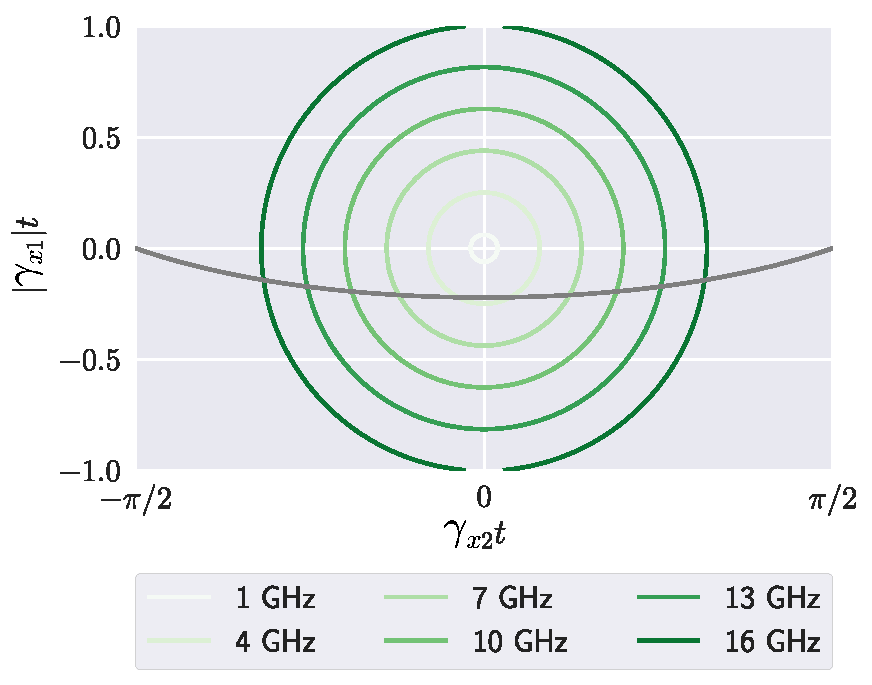
\includegraphics[width=0.48\textwidth]{intro_electro/TE-tan-implicito-zoom}}
	\caption{Curvas de los sistemas de ecuaciones que describen la existencia de ondas superficiales TM y TE, para distintas frecuencias, resuelto para el caso en que el dieléctrico es FR4 ($\epsilon_r = 4.5$).}
	\label{fig:intersecciones-tm-te}
\end{figure}

Obtenidos los valores de $\gamma_{x_1}$ ($\alpha_{x_1}$)y $\gamma_{x_2}$, se obtienen los campos del modo correspondiente de la onda de superficie \cite{Pozar:MwEngineering}. En particular, para el análisis del comportamiento de la impedancia, las expresiones de los campos tangenciales a la interfaz resultan de mayor interés, dado que permiten obtener las impedancias de onda en el aire y el dieléctrico, como se indica en las expresiones \ref{eq:impedancia-no-normalizada-aire} y \ref{eq:impedancia-no-normalizada-FR4}.

\begin{subequations}
	\begin{align}
		H_{y_1} &= A e^{j\gamma_{x_1}(x-t)-j\gamma_{z} z}, &E_{z_1} &= \frac{A \gamma_{x_1}}{\omega \epsilon_0} e^{j\gamma_{x_1}(x-t)-j\gamma_{z} z} &\implies& Z_1 = \frac{\gamma_{x_1}}{\omega \epsilon_0} = j\frac{\alpha_{x_1}}{\omega \epsilon_0}, \label{eq:impedancia-no-normalizada-aire}\\
		H_{y_2} &= 2 B \cos(\gamma_{x_2} x) e^{j\gamma_{z} z}, &E_{z_2} &=  \frac{-2 B \gamma_{x_2} \sin(\gamma_{x_2} x)e^{-j\gamma_{z} z}}{j \omega \epsilon_0 \epsilon_{r_2}} &\implies& Z_2 = \frac{j\gamma_{x_2} \tan(\gamma_{x_2} x)}{\omega \epsilon_0 \epsilon_{r_2}}. \label{eq:impedancia-no-normalizada-FR4}
	\end{align}
\end{subequations}

Normalizando respecto de la impedancia intrínseca del vacío, $\eta_0$, se obtiene, considerando $\theta_t$ el ángulo de transmisión desde el aire al dieléctrico que recubre el plano conductor,

\begin{align}
	\frac{Z_{1}}{\eta_0} &= j\frac{\alpha_{x_1}}{\omega \epsilon_0 \eta_0} = j\frac{\gamma_1 \cos\theta_i}{\omega \epsilon_0 \eta_0} = j\cos \theta_i, \\
	\frac{Z_{2}}{\eta_0} &= j\frac{\gamma_{x_2} \tan \gamma_{x_2} x}{\omega \epsilon_0 \epsilon_{r_2} \eta_0} = j\frac{\gamma_2 \cos\theta_t \tan(\gamma_2 x \cos\theta_t)}{\omega \epsilon_0 \epsilon_{r_2} \eta_0} = j \frac{\cos \theta_t}{\sqrt{\epsilon_{r_2}}}\tan(\gamma_2 x \cos\theta_t).
\end{align}

Una onda incidente desde el aire, para evitar reflexiones y, por lo tanto, radiación desde la superficie que soporta una onda de superficie, debe estar adaptada a la impedancia de superficie que presenta el dieléctrico, que resulta de evaluar $Z_2/\eta_0$ en la superficie, por lo que

\begin{align}
	\label{eq:impedancia-superficie-tm-teorica}
	Z_s^{TM} = j \frac{\cos \theta_t}{\sqrt{\epsilon_{r_2}}}\tan(\gamma_2 t \cos\theta_t).
\end{align}


\begin{figure} [H]
	\centering 
	\subfigure[$Z_s^{TM}$ en función del ancho del dieléctrico, para una permitividad dieléctrica relativa de $4.5$ y en incidencia perpendicular.]{
		\label{fig:zstm-ancho-diel}
		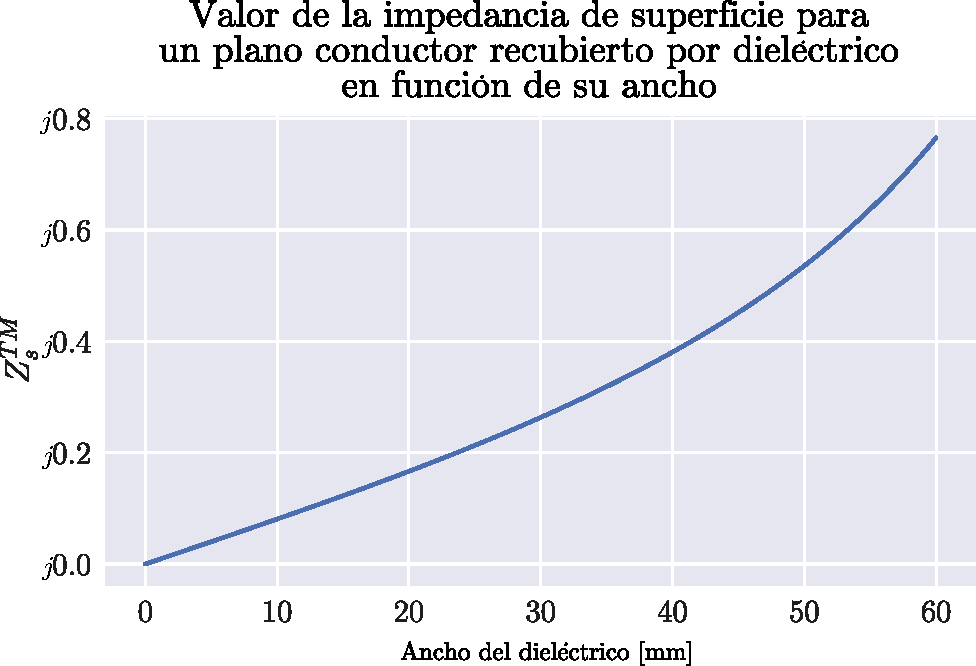
\includegraphics[width=0.45\textwidth]{intro_electro/plot-zstm-funciont.pdf}}
	\hspace{5mm}
	\subfigure[$Z_s^{TM}$ en función de la permitividad dieléctrica, para un ancho de dieléctrico de $1.6\;mm$ y en incidencia perpendicular.]{
		\label{fig:zstm-permit-diel}
		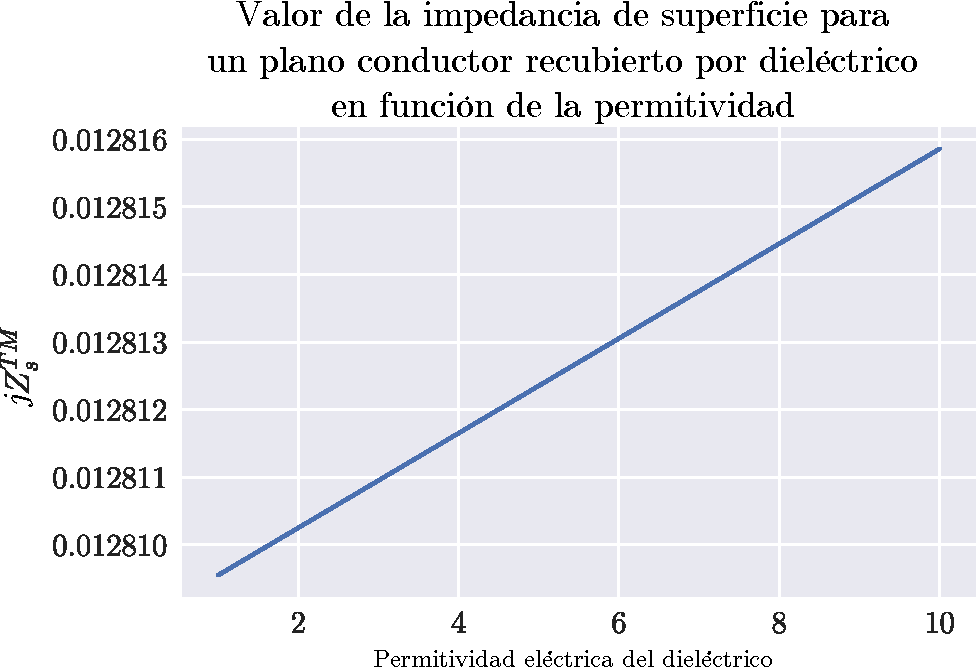
\includegraphics[width=0.45\textwidth]{intro_electro/plot-zstm-funcioner.pdf}}
	\\
	
	\subfigure[$Z_s^{TM}$ en función del ángulo de incidencia, para un ancho de dieléctrico de $1.6\;mm$ y una permitividad de $4.5$.]{
		\label{fig:zstm-angulo-incidencia}
		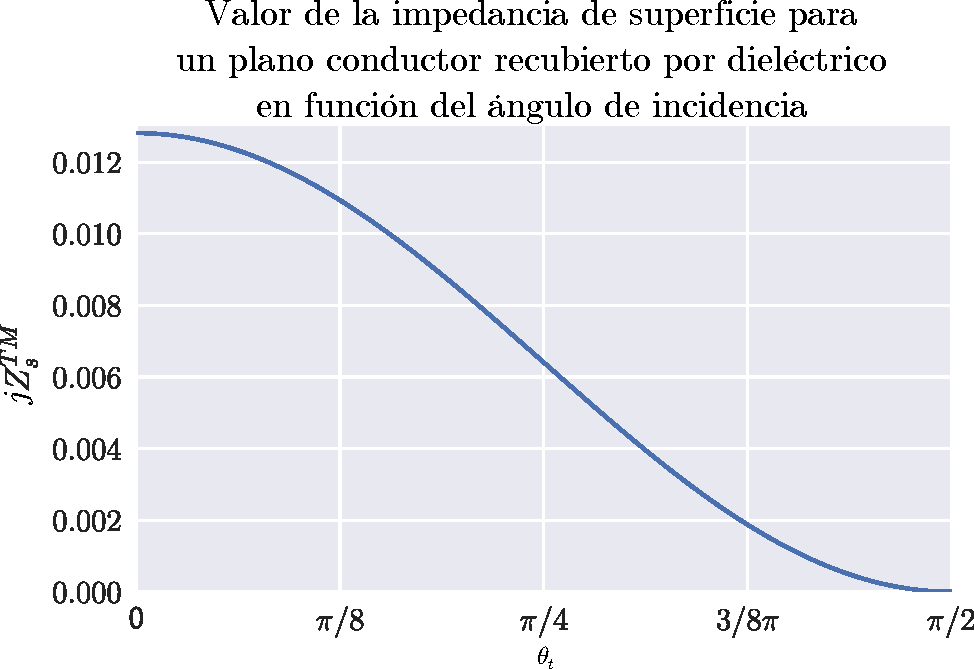
\includegraphics[width=0.45\textwidth]{intro_electro/plot-zstm-funciontheta.pdf}}
	\caption{Valor de la impedancia de superficie en función de sus parámetros.}
	\label{fig:Zstm-parametros}
\end{figure}

%% GRAFICAR!!! \theta_r puede ser obtenida por la ley de snell. Vemos que no es independiente del ángulo de incidencia. Barlow dice que son del mismo orden de magnitud los efectos viejos (prof de penetracion) y los nuevos (coating). Pagina 332. Carita triste.

% Barlow parece contar cosas sobr la velocidad de fase, y más dealnte sobre el lauching y el angulo de brewster complejo. LEER para completar.

Esta impedancia es puramente imaginaria positiva\footnote{Si el dieléctrico presentara pérdidas, existiría también un término real \cite{Barlow:SurfaceWaves}, por lo que, además de facilitar la propagación de ondas de superficie, si el dieléctrico tiene bajas pérdidas, no aumenta la resistencia de superficie. Además, esta componente inductiva se debe sumar al efecto producido por la componente inductiva de la impedancia de superficie del conductor, debida a la existencia de una profundidad de penetración.}, por lo que tiene un comportamiento inductivo, permitiendo la formación de ondas de superficie en modo TM, dado que la constante de atenuación $\alpha_{x_i}, i=1,2$ logra que el campo se concentre cerca de la superficie. Los valores de $\beta_z$ y $\alpha_z$ no se ven modificados, pues el aporte del dieléctrico a la reactancia no es lo suficientemente alto. El ángulo $\theta_t$ se obtiene de las relaciones de Snell (\ref{eq:snell_law_second}), por lo que se deduce que, al contrario que en el caso del conductor sin recubrimiento dieléctrico, el comportamiento es dependiente del ángulo de incidencia, como se muestra en la figura \ref{fig:zstm-angulo-incidencia}. Por otro lado, en la figura \ref{fig:zstm-ancho-diel} se puede observar que el valor de la impedancia crece a medida que aumenta el ancho del dieléctrico, volviéndose más inductiva, de forma similar a la que se da cuando aumenta la permitividad (figura \ref{fig:zstm-permit-diel}).

Para el caso TE, los campos paralelos a la superficie son:

\begin{align}
	E_{y_1} &= A e^{-j\gamma_{x_1}(x-t)-j\gamma_z z}, &H_z &= -\frac{A \gamma_{x_1}}{\omega \mu_0} e^{-j\gamma_{x_1}(x-t)-j\gamma_z z}. \notag \\
	&\implies Z_{1} = -\frac{\gamma_{x_1}}{\omega \mu_0}, \\
	E_{y_2} &= A \sec{(\gamma_{x_2} t)} \cos{(\gamma_{x_2} x)} e^{-j \gamma_z z}, &H_{z_2} &= -\frac{A \gamma_{x_2} e^{j\gamma_z z}}{j\omega \mu_0} \sec{(\gamma_{x_2} t)} \sin(\gamma_{x_2} x), \notag \\
	&\implies Z_{2} = \frac{j\cot(\gamma_{x_2} x)}{\gamma_{x_2} \omega \mu_0}.
\end{align}

Siguiendo la misma metodología que en el caso TM, igualando ambas impedancias, se obtiene

\begin{align}
	Z_s^{TE} = j\frac{\cot(\gamma_2 \cos \theta_t)}{\gamma_2 \cos\theta_t \;\omega \mu_0}.
\end{align}
% Queda explicar qué pasa con el coating -> ubicar también los puntos en el dibujito, para saber por dónde es que nos movimos.


% Engheta, pagina 289
% Rahim (tesis), pagina 28
% Collin, capitulo de Surface waveguides, pag 697
% Paper de Barlow.
% Pozar, pag 138
% Tesis de Kovacs, pagina 8
% Tesis de Zheng, apendice A, pag 48. Interfaces con diel y con metales.


\section{Líneas de transmisión}
\label{sec_lineas_de_transmision}
%%%%

%  Cuando los metamateriales son homogéneos, pueden ser representados por líneas de transmisión unidimensionales, donde la dirección representa cualquier dirección en el material (Caloz, Itoh).

La teoría de líneas de transmisión representa el paso intermedio entre el estudio de campos electromagnéticos y de circuitos de parámetros concentrados, permitiendo considerar el fenómeno de propagación de ondas como una extensión de la teoría de circuitos (aplicable cuando la longitud eléctrica del circuito es mayor a la longitud de onda de operación), o como una solución particular de las ecuaciones de Maxwell \cite{Pozar:MwEngineering}.

Las líneas de transmisión son redes de parámetros distribuidos, donde las corrientes y las tensiones, en contraposición a los circuitos de parámetros concentrados, pueden variar en magnitud y fase, debido a la dimensión física del circuito. El análisis de una línea se puede llevar a cabo estableciendo el comportamiento de los trozos infinitesimales que la componen, dispuestos en cascada para formar la estructura final, de forma que cada uno de ellos se pueda modelar utilizando circuitos de parámetros concentrados independientes de la frecuencia, estableciendo, entonces, impedancias $Z'$ ($\Omega/m$) y admitancias $Y'$ ($S/m$) por unidad de longitud, como se muestra, de forma general, en la figura \ref{fig:TL-equivalente}.

\begin{figure}[htp]
	\centering
	\begin{circuitikz} \draw
		(0,0) -- (1,0)node[midway,scale=2,fill=white]{$\cdots$} -- (7,0)
		(0,2) -- (1,2)node[midway,scale=2,fill=white]{$\cdots$} 
			to [R,l=$R \Delta z$] (3,2)
			to [L,l=$L'_R \Delta_z$] (5,2) 
			to [C,l=$C'_L / \Delta_z$] (7,2)
			to [C,l=$C'_R \Delta_z$] (7,0)
		-- (9,0) to [L,l_=$L'_L / \Delta_z$] (9,2)
		-- (7,2)
		(9,2) -- (11,2)
			to [R,l=$R / \Delta_z$] (11,0)
			-- (9,0)
		(11,0) -- (12,0) -- (13,0)node[midway,scale=2,fill=white]{$\cdots$}
		(11,2) -- (12,2) -- (13,2)node[midway,scale=2,fill=white]{$\cdots$};
	\end{circuitikz}  	
	\caption{Circuito equivalente de porción de línea de transmisión.}
	\label{fig:TL-equivalente}
\end{figure}

La impedancia y la admitancia por unidad de longitud se pueden expresar como indican las expresiones de la ecuación \ref{eq:impedancia-admitancia-TL}. Se debe tener en cuenta que los subíndices R y L se deben al comportamiento de "mano izquierda"\footnote{La expresión "material de mano izquierda´´ fue utilizada por primera vez por físico ruso Viktor Velesago en 1967, cuando propuso la posibilidad de la existencia de materiales en que la propagación de ondas se daría de forma que el campo eléctrico, el campo magnético y el vector de propagación formaran una triada de mano izquierda \cite{Caloz:ElectromagneticMetamaterials}.} o ``mano derecha`` asociado a cada componente. Si $L'_R$ y $C'_R$ son nulos, existe sólo un comportamiento "de mano izquierda", donde las velocidades de fase y de grupo son antiparalelas, y donde tanto la permitividad eléctrica $\epsilon$ como la permeabilidad magnética $\mu$ son negativas, de forma que el índice de refracción también lo sea, dando lugar a una propagación de ondas en sentido inverso. Cuando $L'_L$ y $C'_L$ son nulos, el comportamiento es denominado "de mano derecha", y es el que corresponde a propagación de onda comúnmente analizada. Las componentes que corresponden al comportamiento de mano izquierda son, por sí solas, de existencia física imposibles, dado que las que generan comportamiento de mano derecha aparecen naturalmente por efectos constructivos. Las resistencias del circuito, por otro lado, representan las pérdidas dieléctricas y conductoras.


\begin{align}
\label{eq:impedancia-admitancia-TL}
Z' &= j \left(\omega L'_r - \frac{1}{\omega C'_L} \right), & Y' =j \left(\omega C'_R - \frac{1}{\omega L'_L} \right).
\end{align}

Una descripción completa del análisis del caso general, que describe el comportamiento de numerosos metamateriales, se puede consultar en \cite{Caloz:ElectromagneticMetamaterials}. En adelante se analizará únicamente el caso tradicional, de mano derecha, ya que es el que se aplica al tipo de estructura analizado en este trabajo.

Considerando una línea de transmisión que representa un comportamiento puramente de mano derecha, obteniendo el circuito equivalente de un infinitesimal de línea de la figura \ref{fig:TL-equivalente}, aplicando las leyes de Kirchhoff, dividiendo por $\Delta z$ y aplicando el límite para $\Delta z \rightarrow 0$, para obtener expresiones diferenciales, se obtienen las ecuaciones del telegrafista, expresadas en la ecuación \ref{eq:Telegrafista}, tanto en el dominio del tiempo como de la frecuencia \cite{Fernandez:Electromag}. La solución simultánea de ambas ecuaciones tiene un comportamiento de onda, expresado en \ref{eq:ec-onda-TL}, donde $\gamma$ es la constante de propagación, cuyo valor se expresa en \ref{eq:gamma-tl}.

\begin{align}
	\label{eq:Telegrafista}
	\left. \begin{array}{rr@{\mskip\thickmuskip}l}
	\frac{\partial v(z,t)}{\partial z} & = -R i(z,t) - L \frac{\partial i(z,t)}{\partial t}\\
	\frac{\partial i(z,t)}{\partial z} & = -G v(z,t) - C \frac{\partial v(z,t)}{\partial t}
	\end{array}\right\} \quad \implies \quad \left\{\begin{array}{r@{\mskip\thickmuskip}l}
	\frac{dV(z)}{dz} & = -(R+j\omega L)I(z) \\
	\frac{dI(z)}{dz} & = -(G+j\omega C)V(z).
	\end{array}\right.
\end{align}


\begin{equation}
\begin{aligned}
	\frac{d^2 V(z)}{dz^2} + \gamma^2 V(z) = 0, \\
	\frac{d^2 I(z)}{dz^2} + \gamma^2 I(z) = 0.
\end{aligned}
\label{eq:ec-onda-TL}
\end{equation}

\begin{align}
	\label{eq:gamma-tl}
	\gamma = -j\alpha + \beta = \sqrt{-ZY} = \sqrt{-(R+j\omega L)(G+j\omega C)}.
\end{align}

En base a esta constante de propagación, es posible definir la velocidad de fase $V_p$ como

\begin{align}
	V_p = \frac{\omega}{\beta},
\end{align}

que para el caso sin pérdidas resulta

\begin{align}
	\label{eq:vprop-linea-ideal}
	V_p = \frac{\omega}{\omega \sqrt{LC}} = \frac{1}{\sqrt{LC}}.
\end{align}

Las ecuaciones de onda tienen como solución la superposición de una onda en dirección $+z$ y otra en dirección $-z$, tanto para la tensión como para la corriente, con velocidad de fase $\omega/\beta$. La relación entre las componentes de onda que viajan en dirección positiva se conoce como impedancia característica, $Z_0$, definida, según los parámetros de una línea de transmisión, en la ecuación \ref{eq:TL-impedancia-caracteristica}.
 
\begin{align}
	\label{eq:TL-impedancia-caracteristica}
	Z_0 = \frac{V_0^+}{I_0^+} = \sqrt{\frac{R+j\omega L}{G+j\omega C}}.
\end{align}

Cuando una línea de transmisión es terminada en una impedancia arbitraria $Z_L$, se producen fenómenos de transmisión y reflexión de potencia, de manera análoga al caso de incidencia de campos electromagnéticos sobre interfaces entre medios de impedancias intrínsecas diferentes, analizado en el apéndice \ref{sec:incidencia-onda-plana-interfaz}. Existe, también en este caso, un coeficiente de reflexión $\Gamma$, definido como la relación entre la tensión reflejada y la tensión incidente, como indica la ecuación \ref{eq:coef-reflexion-tl}. Cuando el coeficiente de transmisión es nulo, se dice que la carga está adaptada, de modo que $Z_L = Z_0$.

\begin{align}
	\label{eq:coef-reflexion-tl}
	\Gamma = \frac{V_0^-}{V_0^+} = \frac{Z_L-Z_0}{Z_L+Z_0}.
\end{align}

Si se generaliza el concepto de coeficiente de transmisión a cualquier punto de la línea, y no únicamente al nodo donde se coloca la carga $Z_L$, se obtiene el coeficiente de reflexión para cualquier punto $l$ de la línea a partir del que corresponde al nodo de carga, ubicado en la posición 0, como se indica en la ecuación \ref{eq:coef-reflexion-tl-generalizado}.

\begin{align}
\label{eq:coef-reflexion-tl-generalizado}
\Gamma(l) = \Gamma e^{-2j\gamma l} = \Gamma e^{-2j\beta l} e^{-2\alpha l}.
\end{align}

La impedancia de entrada también varía con la distancia a la carga, de forma que:

\begin{align}
Z_{in} = \frac{V(-l)}{I(-l)} = Z_0 \frac{Z_L +Z_0 \tanh \gamma l}{Z_0 + Z_L \tanh \gamma l}.
\end{align}

En la figura \ref{fig:Zin-Gamma-funcionDistancia-TL} se puede observar una gráfica de $\Gamma$ y $Z_{in}$ en función de la distancia a la carga, para una línea de impedancia característica $Z_0$ de $50 \; \Omega$, con una carga de $100 \; \Omega$, considerando pérdidas y constante de propagación arbitrarias.

\begin{figure}[htp]
	\centering
	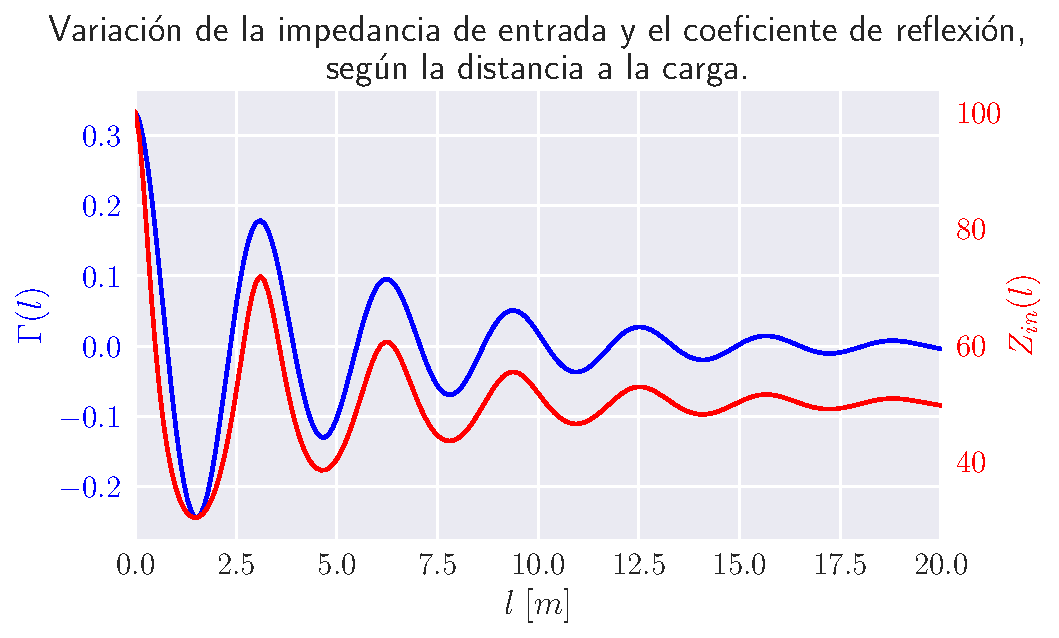
\includegraphics[width=0.8\textwidth]{intro_electro/Zin-Gamma-funcionDistancia-TL.pdf}
	\caption{Impedancia de entrada y coeficiente de reflexión en función de la distancia a la carga, en una línea de transmisión de $50 \Omega$.}
	\label{fig:Zin-Gamma-funcionDistancia-TL}
\end{figure}

En base a este análisis, resulta útil conocer la matriz de transferencia $ABCD$ que corresponde a una línea de transmisión ideal. La misma relaciona las tensiones y corrientes en un nodo con las de otro de forma que

\begin{figure}[htp]
	\centering
	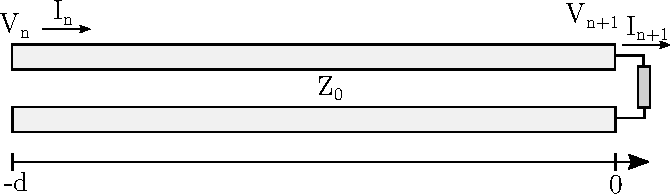
\includegraphics[width=0.8\textwidth]{intro_electro/lineaTransmision-d.pdf}
	\caption{Línea de transmisión con carga.}
	\label{fig:TL-con-carga}
\end{figure}

\begin{align}
\begin{bmatrix}
A & B \\
C & D
\end{bmatrix}
\begin{bmatrix}
i_n \\
v_n
\end{bmatrix}
=
\begin{bmatrix}
i_{n+1} \\
v_{n+1}
\end{bmatrix}.
\end{align}

La deducción de los componentes de la matriz de transferencia requiere del análisis de las ondas incidentes y reflejadas que inciden sobre terminales ubicados a una distancia $d$ de la carga, que puede ser un cortocircuito (para obtener los valores de $B$ y $D$) o un abierto (de donde se pueden deducir los valores de $A$ y $C$).

Dado que la tensión reflejada vista a distancia $d$ de la carga, $V^{-}(d)$, se calcula como $-Z_0 I^{-}$, y que la tensión total sobre dicho nodo resulta de la suma de ambas tensiones (la incidente y la reflejada), para el caso de una carga cortocircuito ($Z_L = 0$), donde la tensión sobre la carga es $V_{n+1} = 0$, resulta que:

\begin{align}
	\Gamma = -1 \implies V(d) = V_n e^{-j\gamma d} - V_n e^{j\gamma d} = 2 j V_n \sin(\gamma d) = B, \\
	I_n (d) = I_n e^{-j\gamma d} + I_n e^{j\gamma d} = 2 I_n \cos(\gamma d) = D.
\end{align}

De forma similar, para el caso de una carga de tipo circuito abierto, $Z_L \rightarrow \infty$, $\Gamma = 1$ y

\begin{align}
V(d) = V_n e^{-j\gamma d} + V_n e^{j\gamma d} = 2 V_n \cos(\gamma d) = A, \\
I_n (d) = I_n e^{-j\gamma d} - I_n e^{j\gamma d} = 2 j I_n \sin(\gamma d) = C.
\end{align}

En forma normalizada, la matriz resulta \cite{Pozar:MwEngineering}

\begin{align}
\label{eq:matriz_transferencia_lineaideal}
\begin{bmatrix}
\cos(\gamma d) & \sin(\gamma d) \\
\sin(\gamma d) & \cos(\gamma d)
\end{bmatrix}.
\end{align}


% Venkateswaran, cap 1.
%%%%
\subsection{Línea \textit{microstrip}}

Algunas de las líneas de transmisión más comunes están basadas en tecnologías de circuitos impresos, entre las que se destacan las \textit{striplines} (donde el dieléctrico circundante al conductor es homogéneo), las líneas \textit{microstrip} (donde el dieléctrico circundante es aire en la mitad superior, y un dieléctrico de mayor permitividad en la mitad inferior), y las guías de ondas coplanares (donde el plano de tierra y la línea de señal comparten la misma cara del sustrato). Algunas de ellas son esquematizadas en la figura \ref{fig:strip-line-technology}. Los costos de fabricación de las mismas suelen ser muy bajos, y ofrecen comodidades para la implantación de componentes discretos, aunque en muchos casos se generan modos indeseados, que pueden ser disminuidos manteniendo el espesor del sustrato en valores despreciables respecto de la longitud de onda, lo que los vuelve frágiles. Además, los sustratos dieléctricos suelen presentar pérdidas que modifican el comportamiento de la señal. Las principales aplicaciones se relacionan con el diseño de filtros microondas, acopladores direccionales, transformadores de impedancia, planos de tierra y redes de distribución de energía de circuitos impresos e integrados \cite{Venkateswaran:Thesis}.


\begin{figure}[htp]
	\centering
	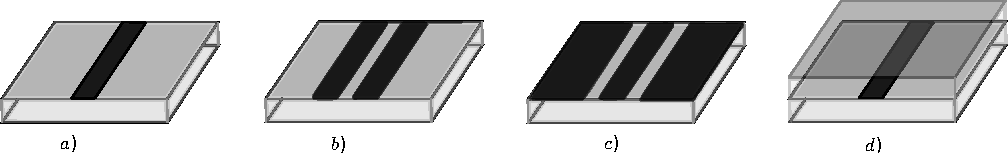
\includegraphics[width=\textwidth]{intro_electro/microstrip-stripline-coplanar.pdf}
	\caption{Tecnologías de líneas de transmisión planares. De izquierda a derecha: \textit{Microstrip}, \textit{twinstrip}, línea coplanar y \textit{stripline}.}
	\label{fig:strip-line-technology}
\end{figure}

Las \textit{striplines}, debido a la homogeneidad del dieléctrico, soportan modos TEM. Las líneas \textit{microstrip}, en cambio, sólo pueden presentar modos TE y TM, aunque en frecuencias bajas tienen un comportamiento que puede denominarse cuasi-TEM, dado que la mayor parte del campo se concentra en el dieléctrico \footnote{Un comportamiento puramente TEM impediría el cumplimiento de la condición de fase en la interfaz, dado que las velocidades de propagación en ambos medios es distinta \cite{Pozar:MwEngineering}}. Un diagrama simplificado de los campos y los parámetros de una línea \textit{microstrip} se muestran en la figura \ref{fig:microstrip-campos}


\begin{figure}[htp]
	\centering
	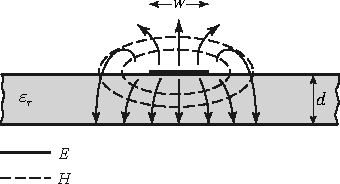
\includegraphics[width=0.5\textwidth]{intro_electro/microstrip-campos.pdf}
	\caption{Campos de una línea \textit{microstrip} [Basado en representación de \cite{Pozar:MwEngineering}].}
	\label{fig:microstrip-campos}
\end{figure}

En general, para simplificar el análisis, se considera que la cinta \textit{microstrip} es una \textit{stripline}, donde el dieléctrico tiene una constante dieléctrica efectiva, menor a la constante dieléctrica del sustrato, pero mayor a la del aire, dependiente del ancho del sustrato, el ancho del conductor y la frecuencia de trabajo. La expresión de esta constante es

\begin{align}
	\epsilon_{eff} = \epsilon_0 \left(\frac{\epsilon_r+1}{2} + \frac{\epsilon_r-1}{2} \left( 1+12 \frac{h}{W} \right)^{-1/2} \right).
	\label{eq:cte-diel-efectiva-microstrip}
\end{align}

\section{Antenas}
\label{subsec_antenas}
%%%%

Una antena es un dispositivo que actúa como fuente de ondas electromagnéticas. Es una interfaz entre el espacio libre y un dispositivo de guiado (como una guía de ondas o una línea de transmisión), y puede ser puede ser modelada como una carga que, en general, está adaptada. Su función es recibir o transmitir energía, usualmente optimizando algunas direcciones, y suprimiendo o disminuyendo su valor en otras, para lo que se utilizan distintas tecnologías, entre las que se destacan las antenas de hilo, de apertura y \textit{microstrip}, muchas veces dispuestas en arreglos y con componentes reflectores \cite{Balanis:Theory}. En este trabajo resultarán de mayor importancia las regiones más cercanas al radiador, y el control del comportamiento de los campos en las mismas modificará el comportamiento en la región de Fraunhoffer.

%%%%
\subsection{Regiones de campo}
\label{subsubsec_regiones_de_campo}
%%%%
El espacio que rodea a una antena se suele dividir en tres regiones: Campo cercano reactivo (donde predominan los campos reactivos), campo de radiación cercano (Fresnel, donde la distribución angular de energía depende de la distancia a la antena) y campo lejano (Fraunhoffer, donde la distribución angular de energía es, en términos prácticos, independiente de la distancia al elemento radiante). En general, se considera que la región de campo lejano se encuentra a distancias mayores a $2D^2/\lambda$, donde D es la máxima dimensión de la antena, y $\lambda$ es la longitud de onda de trabajo.

%%%%
\subsection{Diagramas de radiación}
\label{subsubsec_diag_de_rad}
%%%%
El diagrama de radiación es una representación gráfica o función matemática que representa las propiedades de radiación de una antena como función de las coordenadas espaciales. En general, se especifica para la región de campo lejano, y en función de las coordenadas direccionales $\theta$ y $\phi$, que representan el ángulo de elevación y el azimutal, respectivamente, para una orientación arbitraria del radiador.

En general, se calcula el patrón de potencial o el patrón de campo eléctrico, y se los normaliza respecto de su máximo valor, para luego graficarlos en escala logarítmica o en decibeles.

Sobre el patrón se distinguen lóbulos, clasificados como principal (en la dirección de mayor radiación) y menores (en otras direcciones). El diagrama de radiación de una antena isotrópica, de ser físicamente realizable, se correspondería con una esfera, dado que no existen direcciones privilegiadas. Cuando no existen lóbulos distinguibles en un dado plano, lo cual es común es antenas con simetría cilíndrica, el comportamiento se denomina omnidireccional.
%%%%

\subsection{Impedancia de entrada}
\label{subsec_imp_entrada}
%%%%
La impedancia de entrada de una antena es la que presenta a la línea de transmisión o guía de ondas que la alimenta. En general tiene una componente resistiva y una componente reactiva, de manera que $Z_A = R_A + j X_A$. En general, $R_A$ tiene dos componentes: $R_r$, la resistencia de radiación, y $R_L$, la resistencia de pérdidas. Como en general no coincide con la impedancia característica de la línea de transmisión que la alimenta, se aplican métodos de adaptación de impedancias.
%%%%

\subsection{Arreglos de antenas}
% Ver apunte tesis overleaf

Un arreglo de antenas es un conjunto de antenas dispuestas geométricamente, y alimentadas de manera tal que conformen un único sistema radiante. El primer conjunto de antenas usado extensivamente fue la antena Yagui-Uda, inventada en 1926, cuya fase no puede variarse electrónicamente. Recién durante la Segunda Guerra Mundial se inventaron los conjuntos de antena de fase variable, y a partir de 1950, con la invención de los defasadores de ferrita, la modificación de fase completa fue posible \cite{Stutzman:AntennaTheory}.

El análisis más sencillo del comportamiento de conjuntos de antenas se presenta al analizar uno formado por antenas de iguales propiedades, cuyas amplitudes y fases pueden ser modificados, tanto en transmisión (a través de mecanismos de desfasaje) como en recepción (debido a diferencias e camino y circuitos de desfasaje). En general, el diagrama de radiación se puede calcular en base a la multiplicación del patrón de uno de los elementos y el patrón del arreglo, para el cual se asumen puntos de radiación isotrópicos en la posición de las antenas \cite{Balanis:Theory}.

\begin{figure}[htp]
	\centering
	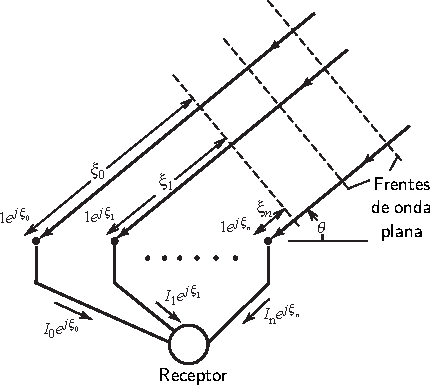
\includegraphics[width=0.5\textwidth]{intro_electro/array-de-antenas.pdf}
	\caption{Incidencia de una onda plana sobre un arreglo de antenas [Basado en la representación del fenómeno en \cite{Balanis:Theory}].}
	\label{fig:rayosincidentes-array}
\end{figure}

El factor de \textit{array}, reemplazando cada elemento por radiadores isotrópicos, se obtiene considerando que una onda plana incide con ángulo $\theta$ sobre el conjunto, como se muestra en la figura \ref{fig:rayosincidentes-array}. Cada elemento es excitado con una fase $\xi_i$, debida a la diferencia de caminos y a las diferencias entre las líneas de transmisión de cada antena, de modo que

\begin{equation}
AF=I_0e^{j\xi_0} + I_1e^{j\xi_1} + ... = \sum_{n=0}^{N-1} I_n e^{j\beta n d cos(\theta)}=\sum_{n=0}^{N-1} I_n e^{jn\Phi}.
\end{equation}

Normalizando y simplificando la expresión, la misma queda

\begin{equation}
	f(\Phi) = \frac{sin(N\Phi/2)}{N sin(\Phi/2)} \qquad (2\pi-\text{periódica}),
\end{equation}

con N la cantidad de elementos radiantes. Se observa que si hay una mayor cantidad de elementos radiantes, los lóbulos, tanto secundarios como primarios, tiende a aumentar. Además, al mismo tiempo, la cantidad de lóbulos secundarios también crece (hay N-1 lóbulos secundarios), al mismo tiempo que disminuye la altura de los mismos \cite{Stutzman:AntennaTheory}.

\subsection{Acoplamiento mutuo}
\label{subsec_acoplamiento}
%%%%
Cuando se considera acoplamiento mutuo entre los elementos del \textit{array}, la multiplicación del patrón de radiación por el patrón del arreglo ya no es válida. Los elementos interaccionan entre sí y alteran sus corrientes, y por lo tanto sus impedancias. La radiación de una antena induce corrientes sobre las antenas cercanas, que también radian e influyen sobre la corriente de la primer antena. Es un efecto de campo cercano.

La impedancia de entrada de un elemento aislado en el espacio se denomina ``Impedancia de elemento aislado", o simplemente impedancia de antena. La impedancia de entrada de una antena que está dispuesta en un ambiente con elementos activos se denomina ``impedancia activa", y varía según las excitaciones a las que se someta al arreglo de antena. En general, la caracterización de los elementos radiantes sometidos a efectos de acoplamiento mutuo consisten en la obtención de la ``impedancia pasiva", que se logra excitando un elemento y conectando a cargas adaptadas los demás.

Hay 3 efectos responsables del acoplamiento mutuo en arreglos de antenas:

\begin{itemize}
	\item Acoplamiento espacial entre elementos.
	\item Acoplamiento espacial por \textit{scattering} en elementos cercanos.
	\item Acoplamiento por la red de alimentación, que puede ser minimizado usando técnicas de acoplamiento apropiadas en cada elemento.
\end{itemize}

Si el acoplamiento en la red de alimentación se minimiza, se puede considerar que cada antena está alimentada independientemente con una tensión $V_m^g$, cuyo generador tiene una impedancia asociada $Z_m^g$. Sobre la antena se genera una diferencia de tensión $V_m$, y una corriente $I_m$, que incluye los efectos de acoplamiento. Un \textit{array} de N elementos es entonces una red de N puertos, representada por la ecuación \ref{eq:Matriz_impedancias_mutuas}, donde todos los elementos que pertenecen a la diagonal de la matriz $Z$ son las impedancias de elemento aislado, mientras que los elementos fuera de la diagonal representan las impedancias mutuas $Z_{mn}$, que no es más que la tensión impresa sobre el elemento $m$ por la corriente $n$, cuando todos los demás terminales están a circuito abierto ($Z_{mn}=V_m/I_n |_{I_i=0\; \forall i \neq n}$, lo que significa que la corriente es nula para todo el cuerpo de la antena). En general estos cálculos se realizan de forma numérica, tras las correspondientes simulaciones, y considerando a las antenas en modo transmisor \cite{Fano:CouplingReceiving}.

\begin{equation} \label{eq:Matriz_impedancias_mutuas}
\begin{bmatrix}
V_1 \\ V_2 \\ \vdots \\ V_N
\end{bmatrix}
=
\underbrace{\begin{bmatrix}
	Z_{11} & Z_{12} & \cdots & Z_{1N} \\
	Z_{12} & Z_{22} & \cdots & Z_{2N} \\
	\vdots & \vdots & \cdots & \vdots \\
	Z_{1N} & Z_{2N} & \cdots & Z_{NN} \\
	\end{bmatrix}}_{Z}
\begin{bmatrix}
I_1 \\ I_2 \\ \vdots \\ I_N
\end{bmatrix}.
\end{equation}

Si suponemos que la antena no excitada tiene una impedancia de carga $Z^g_j$ sobre sus terminales (y que el generador de esa antena está apagado, $V^g_j=0$), la corriente generada sobre el elemento $j$ debido a la radiación del elemento $i$ será tal que $V_j=-Z^g_j I_j$, por lo que

\begin{equation} \label{eq:impmutua}
V_j = -Z^g_j I_j = Z_{jj}I_j + \sum_{i=1, i \neq j}^{N} Z_{ji}I_i.
\end{equation}

En el caso en que se consideren sólo dos antenas, de la ecuación \ref{eq:impmutua} para dos elementos, podemos obtener la expresión de la corriente en el segundo elemento, que da lugar a la expresión de la impedancia total vista por el primer elemento, por efecto propio y de la radiación del segundo, como muestra la ecuación \ref{eq:impedanciamutua}, donde se asumió que la matriz Z es simétrica, y que permite deducir la ecuación \ref{eq:impedanciaAntenaEnArray}, que es la impedancia de entrada de cada elemento, en función de impedancias mensurables.

\begin{equation}
	\label{eq:impedanciamutua}
	\left\{
	\begin{aligned}
		V_1 &= Z_{11} I_1 + Z_{12} I_2 \\
		V_2 = -Z^g_2 I_2 &= Z_{22} I_2 + Z_{21}I_1.
	\end{aligned}
	\right.
\end{equation}

\begin{align}
	\label{eq:impedanciaAntenaEnArray}
	I_2 = \frac{-Z_{21}I_1}{Z_{22}+Z^g_{2}} = \frac{-Z_{12}I_1}{Z_{22}+Z^g_{2}}  \quad \implies \quad
	\frac{V_1}{I_1} = Z_1 = Z_{11} - \frac{(Z_{12})^2}{Z_{22}+Z^g_2}.
\end{align}

%Paper de fano y el cordobeés.
%%%%
%\subsection{Dieléctricos y pérdidas dieléctricas}
%\label{subsec_dielectricos}
%%%%%%%%%%%%%%%%%%%%%%%%%%%%%%%%%%%%
%%%%%%%%%%%%%%%%%%%%%%%%%%%%%%%%%%%%
%%%%%%%%%%%%%%%%%%%%%%%%%%%%%%%%%%%%
%%%%%%%%%%%%%%%%%%%%%%%%%%%%%%%%%%%%
%%%%%%%%%%%%%%%%%%%%%%%%%%%%%%%%%%%%
%\lipsum[2]
% LibroSinNombre, pagina 816
%%%%%%%%%%%%%%%%%%%%%%%%%%%%%%%%%%%%

\subsection{Antenas \textit{microstrip}}
\label{subsec_antenas_microstrip}
%%%%
Las antenas \textit{microstrip} cumplen varias de las especificaciones más importantes que imponen las diversas aplicaciones de antenas: Pueden ser pequeñas, tienen bajo peso, son económicas y fáciles de fabricar, y tienen bajo perfil, lo que permite adaptarlas a numerosos diseños. Suelen, sin embargo, tener un alto Q, ya que funcionan debido a sus propiedades resonantes, suelen tener baja eficiencia, son de baja potencia, y presentan polarización impura.

En general, el diseño de una antena \textit{microstrip} se realiza de forma tal que el máximo de radiación se concentre en la dirección normal al parche (\textit{broadside}), aunque también es posible lograr radiación en dirección paralela al mismo (\textit{end-fire}), dependiendo de la geometría elegida. El sustrato elegido para la fabricación suele influir en el ancho de banda y la eficiencia: Una mayor permitividad dieléctrica genera una menor eficiencia, un menor ancho de banda y un menor acoplamiento con elementos cercanos, debido a que los campos se encuentran contenidos en el sustrato.

Existen múltiples formas de alimentación de una antena \textit{microstrip}, entre las que se destacan la línea microstrip de alimentación, que suele dar lugar a radiación espuria y a polarización cruzada, debido a la asimetría que impone; y la conexión directa de cable coaxil, donde el conductor central del mismo se conecta en un punto del parche, y la malla se conecta al plano de tierra que funciona como reflector, ubicado en la cara opuesta del sustrato.

Existen varios métodos de análisis de antenas \textit{microstrip}, entre los que se destacan, por su sencillez, el modelo de líneas de transmisión y el modelo de cavidades resonantes, principalmente aplicables a parches rectangulares, que son los de interés en este trabajo. Sin embargo, estos métodos no consideran acoplamiento mutuo ni ondas de superficie, por lo que resultan incompletos \cite{Pozar:InputImpedanceMutualCoupling}.
%%%%
\subsubsection{Modelo de líneas de transmisión}
\label{subsubsec_microstrip_modeloLineas}
%%%%
El modelo de líneas de transmisión es el más sencillo y el que ofrece una mayor intuición física, ya que usa los conceptos fundamentales de líneas \textit{microstrip}. Consiste en considerar a la antena como dos aperturas radiantes de ancho $W$ y altura $h$ separadas una distancia $L$ por una línea de transmisión de impedancia característica conocida $Z_0$, cada una de las cuales puede ser representada, en el modelo, como una conductancia $G$ y una susceptancia $B$, como se indica en la figura \ref{fig:circuito-equivalente-antena-ms}, donde la admitancia y la susceptancia se obtienen del modelo de apertura radiante, que puede consultarse en \cite{Balanis:Theory}.

\begin{figure}[htp]
	\centering
	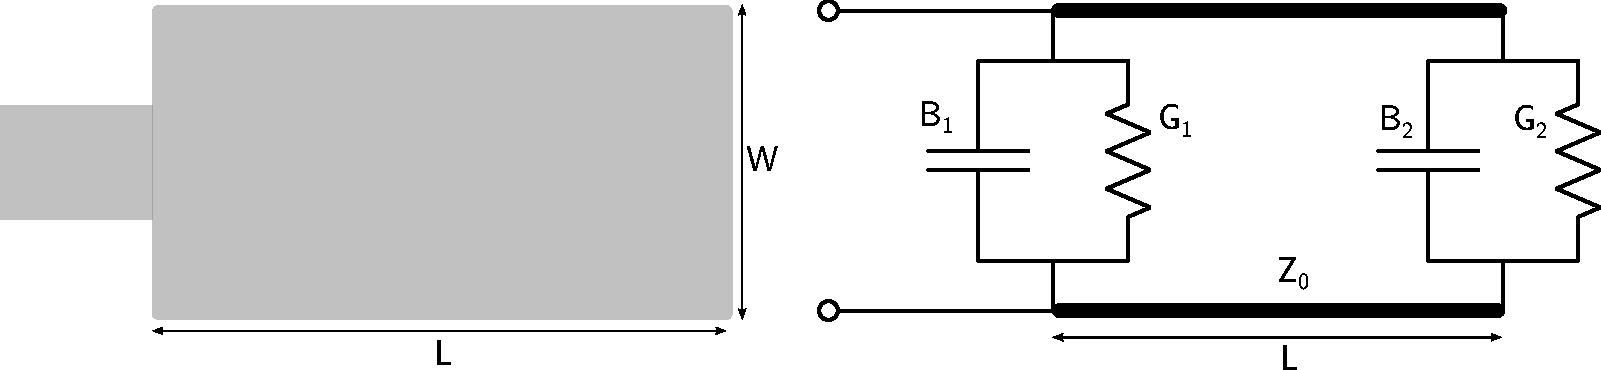
\includegraphics[width=0.8\textwidth]{intro_electro/circuito-equivalente-antena-ms.pdf}
	\caption{Circuito equivalente, según el modelo de líneas de transmisión, de una antena \textit{microstrip}.}
	\label{fig:circuito-equivalente-antena-ms}
\end{figure}



Al igual que en el caso de las líneas \textit{microstrip}, se debe considerar una constante dieléctrica efectivo $\epsilon_{r_{eff}}$, que depende no sólo del ancho del sustrato, sino también de la frecuencia, debido a que a mayor frecuencia hay una mayor concentración de campo sobre el dieléctrico, otorgando mayor prevalencia a la constante dieléctrica del sustrato que a la del aire circundante en el cálculo de la constante efectiva. La expresión es la misma utilizada para líneas \textit{microstrip} (ecuación \ref{eq:cte-diel-efectiva-microstrip}), siempre y cuando $W>h$.

El efecto de \textit{fringing} en los bordes del parche, que da lugar a un aumento del tamaño eléctrico, se modelan mediante la consideración de una extensión en la línea de transmisión que une a las aperturas radiantes, en función de la altura del sustrato. El cambio en la extensión de la línea de transmisión sugiere un cambio en la frecuencia de resonancia de la antena, al mismo tiempo que un mayor ancho de banda, sin una modificación del tamaño físico. En la ecuación \ref{eq:deltaL-antena-microstrip} se muestra una expresión aproximada de la variación del tamaño eléctrico, de forma que la longitud efectiva de la línea de transmisión resulta $L_{eff} = L + 2 \Delta L$. Esta expresión se utiliza para la obtención de la frecuencia de resonancia, como indica la expresión \ref{eq:frec-resonancia-modelo-linea-microstrip} para el modo dominante, $TM_{010}$.

\begin{align}
	\Delta L = h\; 0.412 \frac{(\epsilon_{eff}+0.3)(W/h + 0.264)}{(\epsilon_{eff}-0.258)(W/h +0.8)}.
	\label{eq:deltaL-antena-microstrip}
\end{align}

\begin{align}
	f_{{r}_{010}} = \frac{v_p}{\lambda} = \frac{c/\sqrt{\epsilon_{r_{eff}}}{2*L_{eff}}} = \frac{1}{2 L_{eff} \sqrt{\epsilon_{eff}} \sqrt{\mu_0 \epsilon_0}} = \frac{1}{2 (L+2 \Delta L) \sqrt{\epsilon_{eff}} \sqrt{\mu_0 \epsilon_0}}.
	\label{eq:frec-resonancia-modelo-linea-microstrip}
\end{align}

La impedancia de entrada de una antena \textit{microstrip} depende fuertemente de la posición de la alimentación, además de los valores de $G$ y $B$ de los \textit{slots} radiantes \cite{Balanis:Advanced}. Cuando la alimentación se realiza mediante una cinta \textit{microstrip}, se suele terminar la misma en el interior del parche, a una distancia $y_0$ del borde, como se indica en la figura \ref{fig:antema-microstrip-inset}, permitiendo una mejor adaptación, aunque introduciendo una capacidad de juntura que afecta a la frecuencia de resonancia. La distancia del punto de alimentación al borde del parche será menor a la mitad de la longitud total del parche, en lo que se identificó como "zona de adaptación'' en la misma figura.

\begin{figure} [H]
	\centering
	\subfigure[]{
		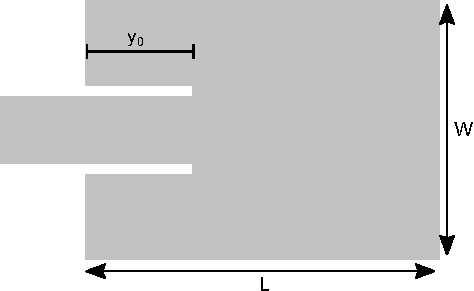
\includegraphics[width=0.48\textwidth]{intro_electro/antena-inset-drawing.pdf}}
	\subfigure[]{
		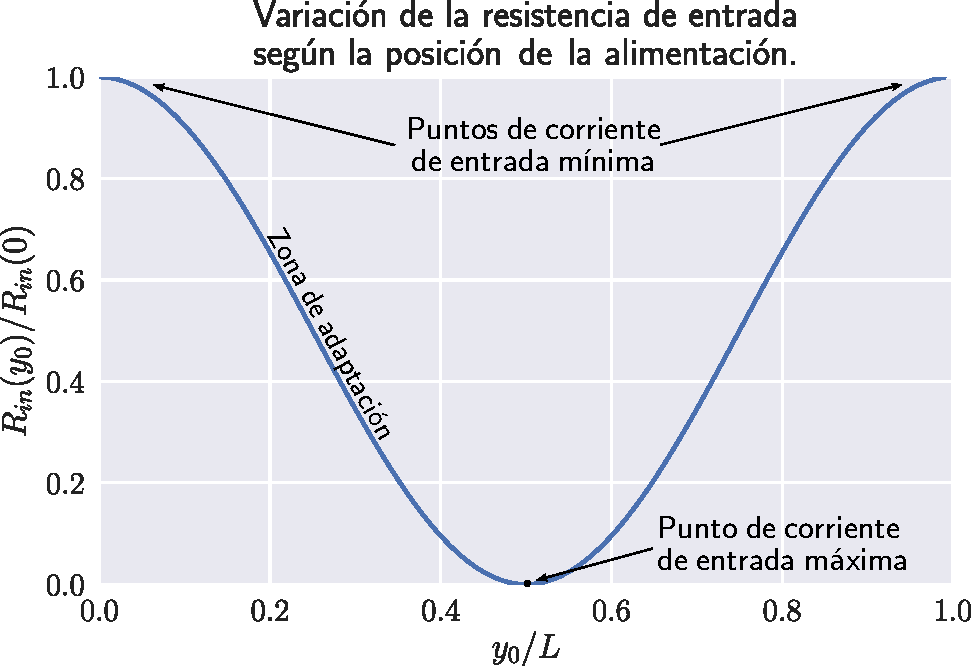
\includegraphics[width=0.48\textwidth]{intro_electro/plot-RinInset.pdf}}
	\caption{Esquema y gráfica del comportamiento de la impedancia de entrada según la posición de la alimentación.}
	\label{fig:antema-microstrip-inset}
\end{figure}


El factor de antena, el ancho de banda y la eficiencia son valores interdependientes, y entre ellos se presenta una relación de compromiso. El factor de antena representa las pérdidas de la misma, en general dominadas por la radiación (relacionada a la conductancia asociada a las aperturas radiantes), la conducción (en función de la conductividad del metal), las pérdidas dieléctricas (expresada según la tangente de pérdidas) y las ondas de superficie (despreciables si el sustrato es demasiado fino). Además, se debe tener en cuenta la adaptación de la antena, que limita fuertemente el ancho de banda de uso. En general, se observa que \cite{Balanis:Theory} a mayor volumen de la antena, el ancho de banda aumenta. Un aumento de la permitividad dieléctrica genera una disminución del ancho de banda, debida a la disminución de los campos de borde (\textit{fringing}) y una disminución de la eficiencia de radiación, dado que da lugar a antenas de menor tamaño. Un sustrato de mayor constante dieléctrica, entonces, da lugar a antenas de menor volumen, lo cual genera un menor ancho de banda.

% LibroSinNombre, pahgina 534
%%%%
\subsubsection{Modelo de cavidades multimodo}
\label{subsubsec_microstrip_modeloCavidades}
%%%%

El modelo de cavidad resonante se utiliza principalmente para predecir el comportamiento en modos superiores de la antena. Para ello se considera que la región dieléctrica bajo el parche consiste en una cavidad cargada dieléctricamente, limitada por conductores eléctricos en las caras superior e inferior, y por conductores magnéticos en las caras laterales. Esta configuración conlleva a una impedancia de entrada puramente reactiva, incompatible con el comportamiento radiante del sistema, pero consistente con el comportamiento de otros parámetros. Para considerar las pérdidas por radiación, se añaden efectos de pérdidas dentro de la cavidad, relacionados con el factor de antena correspondiente.

La consideración de paredes laterales como conductores magnéticos deviene de la consideración de la disposición de las cargas sobre el parche conductor y sobre el plano de tierra, donde se asume que el espesor del dieléctrico es lo suficientemente pequeño como para que no se presenten modos superiores sobre el eje vertical. Las cargas sobre la cara inferior del parche son atraídas por las cargas opuestas correspondientes en el plano de tierra, y su concentración genera una repulsión, hacia la cara superior, a otras cargas de la misma polarización, generando una corriente superficial en cada cara, como se indica en la figura \ref{fig:corrientes-microstrip}. Al disminuir el ancho del sustrato, el efecto de atracción del plano del tierra supera, en magnitud, al efecto de repulsión por la concentración de cargas en la cara inferior del parche, por lo que el flujo decrece, pudiendo considerarse nulo. Dado que el flujo de cargas, a través de los bordes, entre la cara superior y la inferior del parche metálico dispuesto sobre el sustrato, es el responsable del campo magnético tangencial a los bordes, la desaparición de dicho flujo disminuiría considerablemente este campo, permitiendo asumir que las paredes se comportan como conductores magnéticos. La baja altura del sustrato, además, permite considerar sólo las configuraciones TM para las frecuencias de interés, dado que, como se explicó antes, $h<<\lambda$.

\begin{figure}[htp]
	\centering
	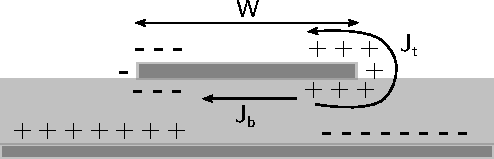
\includegraphics[width=0.4\textwidth]{intro_electro/corrientes-microstrip.pdf}
	\caption{Corrientes sobre el parche en una antena \textit{microstrip}, según el modelo de cavidad.}
	\label{fig:corrientes-microstrip}
\end{figure}

La obtención de los campos se detalla en \cite{Balanis:Advanced}, donde, considerando las hipótesis descriptas antes, asumiendo que el vector de potencial $\vec{A}$ tiene que cumplir la ecuación de Helmholtz (\ref{eq:Helmholtz}), y utilizando separación de variables, se obtienen soluciones para distintos modos, todos transversales magnéticos, con frecuencias de resonancia dadas por \ref{eq:frecRes-modosSup-microstripAntenna}, donde $n$, $m$ y $p$ son los índices del modo. El modo dominante, dado que $h < L$ y $h < W$, es el $TM_{010}$, cuya distribución de campos se muestra en la figura \ref{fig:distribucion-campos-microstrip}.
 
\begin{align}
	(f_r)_{nmp} = \frac{1}{2 \pi \sqrt{\mu \epsilon}} \sqrt{\left(\frac{m\pi}{h}\right)^2 + \left(\frac{n\pi}{L}\right)^2 + \left(\frac{p\pi}{W}\right)^2}.
	\label{eq:frecRes-modosSup-microstripAntenna}
\end{align}

\begin{figure}[htp]
	\centering
	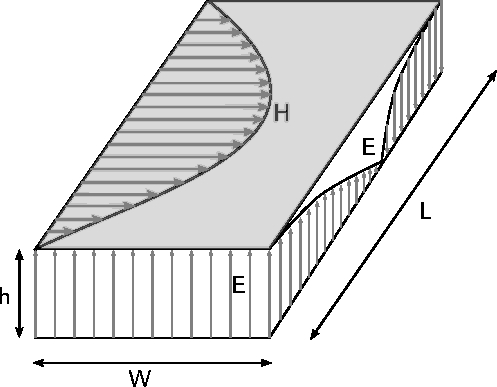
\includegraphics[width=0.4\textwidth]{intro_electro/distribucion-campos-microstrip.pdf}
	\caption{Distribución de campos eléctrico y magnético en la cavidad de \textit{microstrip}, para el modo $TM_{010}$.}
	\label{fig:distribucion-campos-microstrip}
\end{figure}

A pesar de que hay 4 aperturas en una antena \textit{microstrip} rectangular, sólo 2, las radiantes, aportan significativamente a la radiación, dado que lo radiado por las otras dos se cancelan sobre los planos principales. Las paredes separadas aproximadamente $\lambda/2$ tienen campos en direcciones opuestas en el mismo momento, por lo que se suman en la dirección normal al parche, dando lugar a un comportamiento \textit{broadside}.

Un aspecto importante del análisis por el modelo de cavidad radica en las densidades de corriente equivalentes. Según lo descripto antes, existe una corriente, $\vec{J}$, sobre la superficie del parche. Debido a que la polarización es TM, sobre las aperturas radiantes laterales debe existir también una densidad de corriente eléctrica, $\vec{J}_s$, y una densidad de corriente magnética, $\vec{M}_s$, de modo que, en función de los campos en las aperturas,

\begin{align}
	\vec{J}_s &= \hat{n} \times \vec{H}_a, & \vec{M}_s = - \hat{n} \times \vec{E}_a
\end{align}

Según las hipótesis dadas antes, y como se muestra en la figura \ref{fig:distribucion-campos-microstrip}, la magnitud del campo magnético tangencial a las paredes es despreciable, de modo que la corriente sobre las paredes, $\vec{J}_s$, también lo es. La corriente sobre el parche, debido a la baja distancia con el plano de tierra, es baja, por lo que también puede considerarse despreciable. De esta forma, la única densidad de corriente apreciable es $\vec{M}_s$. El efecto del plano de tierra se puede tener en cuenta considerando teoría de imágenes. Según la misma, dado que se trata de un conductor eléctrico, las corrientes magnéticas imagen tienen el mismo sentido que las originales, de modo que la densidad de corriente magnética equivalente resulta el doble que la original, como se expresa en la ecuación \ref{eq:densidad-de-corriente-caras-laterales-microstrip}, y se observa en la figura \ref{fig:densidad-corriente-microstrip}.

\begin{align}
	\label{eq:densidad-de-corriente-caras-laterales-microstrip}
	\vec{M}_s = -2 \hat{n} \times \vec{E}_a.
\end{align}

\begin{figure}[htp]
	\centering
	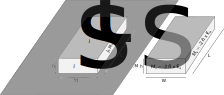
\includegraphics[width=0.8\textwidth]{intro_electro/distribucion-corrientes-microstrip}
	\caption{Densidades de corrientes eléctricas y magnéticas en una antena \textit{microstrip}.}
	\label{fig:densidad-corriente-microstrip}
\end{figure}

Se puede considerar, entonces, que cada apertura actúa como un dipolo magnético con densidad de corriente $\vec{M}_s$. Cuando las aperturas están separadas una distancia de $\lambda/2$, forman un arreglo de dos elementos, que tiene un comportamiento \textit{broadside}.

% Pozar, resonadores, capitulo 6
%%%%

\subsection{Acoplamiento mutuo en antenas \textit{microstrip}}
\label{subsec_acoplamiento_microstrip}
%%%%
El acoplamiento mutuo está determinado principalmente por los campos que existen sobre la interfaz dieléctrico-aire: la onda espacial (decrece como $1/\rho$), los campos cercanos de superior (decreciendo como $1/\rho^2$), la onda de superficie (con dependencia de tipo $1/\rho^{1/2}$) y las ondas de tipo \textit{leaky} (con dependencia del tipo $e^{-Q}/e^{1/2}$) \cite{Balanis:Advanced}. A mayor distancia del elemento radiante fuente, las ondas de superficie son las que tienen carácter dominante, siempre que en esa dirección existan \cite{Alexopoulos:PrintedDipoles}. En general, si la distancia entre los elementos radiantes es grande (mayor a $0.8 \lambda$), la influencia de las ondas de superficie es baja y el acoplamiento es por tanto bajo. Aún así, si el conjunto es grande, la suma de los efectos de los distintos parches puede dar lugar a efectos de acoplamiento significativos, incluso entre elementos no adyacentes \cite{Dodov:SurfaceWavesImpact}. Como en todo conjunto de antenas, el acoplamiento mutuo es función, además de la distancia, de la posición entre los elementos radiantes.

En un \textit{array} planar de antenas se deben considerar la amplitud y la fase de la onda incidente. Si se ubican en forma colineal sobre el plano anche, el acoplamiento mutuo entre las antenas es menor al que se observa si se ubican de forma colineal sobre el plano E (figura \ref{fig:acomplamientoEyH}, \cite{VanLil:TLModelCoupling}, \cite{Pozar:InputImpedanceMutualCoupling}), y el aumento de la distancia entre los parches reduce el acoplamiento \cite{Dodov:SurfaceWavesImpact}. Si los elementos se ubican en forma colineal sobre el plano E, el decrecimiento del parámetro $S_{12}$ es mucho más lento, debido a la presencia de ondas de superficie, comenzando a partir del modo TM, que no posee frecuencia de corte inferior, y aumentando con la aparición de modos TE y TM de orden superior, fruto del aumento de espesor del sustrato y el crecimiento de la constante dieléctrica \cite{Alexopoulos:PrintedDipoles}. La ubicación sobre el plano H genera que las ondas responsables del acoplamiento sean de polarización TE, mientras que la ubicación sobre el plano E genera que las mismas sean de polarización TM, que es la polarización dominante en las antenas \textit{microstrip}. Un aumento en el ancho del sustrato permitiría la aparición de modos TE, generando un mayor acoplamiento en el arreglo sobre el plano H.

\begin{figure}[htp]
	\centering
	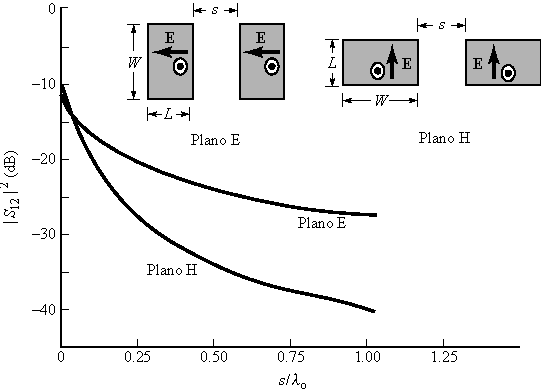
\includegraphics[width=0.8\textwidth]{intro_electro/pozar-acoplamiento.pdf}
	\caption{Acoplamiento mutuo entre antenas \textit{microstrip}, para posición colineal en plano E y plano H. Parámetros: W: 10.57 cm, L: 6.55 cm, h: 0.1588 cm, $\epsilon_r$: 2.55, $f_r$: 1.410 MHz. Fuente: D. M. Pozar, " Input impedance and mutual coupling of rectangular microstrip antennas", IEEE Trans. Antennas Propagat. Vol AP-30, No. 6. Noviembre, 1982.}
	\label{fig:acomplamientoEyH}
\end{figure}

Según \cite{Dodov:SurfaceWavesImpact}, los efectos de onda de superficie son importantes cuando el valor de $\epsilon_r$ del sustrato es alto, y si las pérdidas son bajas, la onda de superficie se mantiene en un valor estable cuando se aumenta la distancia \cite{Gonzalo:PerformancePBG}. Esto hace que el acoplamiento mutuo entre las antenas sea mayor, porque existe una onda de superficie notoria. Por otro lado, según \cite{Penard:MutualCouplingMicrostrip}, si el ancho del dieléctrico es bajo, las ondas de superficie son despreciables. Para separaciones pequeñas, los efectos de campo cercano son los que dominan; en la zona intermedia ($0.4\lambda  < d <  0.8 \lambda$), los efectos de la onda espacial directa son visibles, y en la zona más lejana sólo son reconocibles los efectos originados por las ondas de superficie \cite{Alexopoulos:PrintedDipoles}.

La búsqueda de antenas de menor tamaño (aumentando la constante dieléctrica del sustrato) y mayor ancho de banda (aumentando el ancho del dieléctrico) tiene como obstáculo la relación de compromiso con el acoplamiento causado por ondas de superficie, que son amplificadas cuando la constante dieléctrica aumenta o el sustrato es de mayor altura. En el caso de los llamados \textit{phased arrays} de antenas \textit{microstrip}, el acoplamiento mutuo genera, además de modificaciones en el diagrama de radiación, una limitación en el ángulo de escaneo y puntos ciegos \cite{Iluz:PhasedArray}.

%%%%
% LibroSinNombre, pagina 562 y 631




\chapter{Fundamentos de estructuras de EBG}
\label{cap_fundamentos}
\lhead{Capítulo \ref{cap_fundamentos}. \emph{Fundamentos de EBG}} 
%%%%%%%%%%%%%%%%%%%%%%%%%%
%%  Capítulo 2: Fundamentos de estructuras de banda prohibida electromagnética (EBG)}  %%
%%%%%%%%%%%%%%%%%%%%%%%%%%

%%%%
\section{Reseña histórica: Metamateriales, materiales periódicos y EBGs}
\label{sec_resenia_metamateriales}
%%%%
% EBGs in Antennas, Rahmat (libro). Pagina 2.
% Explicación de los métodos de análisis
% Uso para low profile antennas
% Engheta, pag 215
% Caloz, ^pag 17
% Caloz Pag 20
% Caloz pag 83, diferencia con filtros
% Pozar, pag 380
% Pozar, p 424. Stepped impedance filters.
% Pozar, bandstop filter design, pag 440
% Tabla interesante: Baccarello, Paulotto, impreso.
% stack de capas o cristal? Brown, McMahon, Parker. Ademas linda foto.
% Relación con soft-hard surfaces. Gao, chen, wang, yang-
% Discusión terminológica: Oliner.
% ITOH, Pediodic structures.
% DGS, tesis de ABIDIN, pag2. Tiene intro histórica.
% ABIDIN, tesis, pagina 16: Def de EBG. imagen interesante.
% Venkateswaran, algunos ejemplos de EBGs.
% Importancia de EBGs. Venkateswaran tesis, pag 1.
% Algo de intro: Pagina 4, tesis Zheng.

Los EBG (Materiales de banda prohibida electromagnética, \textit{Electromagnetic Bandgap Materials}), PBG (Materiales de banda prohibida fotónica, \textit{Photonic Bandgap Materials}) o cristales fotónicos son un tipo de estructura artificial, dieléctrica o metalodieléctrica, con capacidades para controlar ondas electromagnéticas \cite{Engheta} a partir de una variación periódica en el espacio de la constante dieléctrica, permitiendo que las mismas se propaguen sólo en direcciones determinadas, o impedir su propagación completamente. Esta capacidad proviene de su estructura de banda prohibida electromagnética, que surge en analogía al concepto de banda prohibida electrónica, que controla el movimiento de ondas de electrones que viajan en un potencial periódico cristalino.

En 1946, Louis Brillouin publicó su libro sobre ondas mecánicas, "\textit{Wave propagation in periodic structures: Electric filters and crystal lattices}" \cite{Brillouin:WavePropagation}, donde demostró que un arreglo periódico impone restricciones a los vectores de onda $k$ que pueden propagarse por él, dado que da lugar a condiciones de contorno para los modos permitidos. Aquellas ondas que no cumplieran las condiciones de borde impuestas, no podrían propagarse. La propagación de ondas sobre superficies periódicas había comenzado a estudiarse, para ondas electromagnéticas, con anterioridad al trabajo de Brillouin, aunque a partir del mismo se formalizó el desarrollo de las aplicaciones para microondas.

En 1968, el físico ruso Viktor Veselago describió por primera vez, de forma teórica, la posibilidad de que existieran materiales con índice de refracción negativo, denominados LHS (\textit{Left Handed Materials}, materiales de mano izquierda), con permitividad eléctrica y permeabilidad magnética negativas, de modo que la velocidad de fase de una onda que se propagara por ese medio fuera antiparalela a la velocidad de grupo. Treinta años más tarde, Pendry propuso la primera forma de fabricación de un medio con esas características en una banda limitada de frecuencia, utilizando SSRs (Split-ring resonators, resonadores de aro dividido), responsables de la permeabilidad magnética negativa, y cables conductores, responsables de la permitividad eléctrica negativa. Recién en el año 2000 se construyó el primer metamaterial sobre las propuestas de Pendry, y varios experimentos confirmaron refracción negativa en los mismos.

La primera descripción de estructuras dieléctricas periódicas con una banda prohibida completa fue dada, en 1990, por Ho, Chan y Soukoulis, en Iowa, Estados Unidos, quienes propusieron un arreglo periódico de esferas dieléctricas, dispuestas en forma de capas. Para un rango amplio de radios de esferas, el efecto de banda prohibida se daba en todas direcciones. Hacia fines de la década de 1980, Yablonovitch divisó una estructura cristalina simétrica de más fácil fabricación, que consistía en la producción de tres agujeros cilíndricos en un prisma dieléctrico, repetido periódicamente. Demostró, además, usando dichas estructuras, que la existencia de una banda prohibida electromagnética podía ser predicha teóricamente, en base, principalmente, a la constante de periodicidad del dieléctrico artificial.

Los trabajos de Yablonovitch y Pendry se hicieron sobre estructuras con banda de interés en microondas, pero bajo modelos fotónicos, gracias a la linealidad de las ecuaciones de Maxwell, lo que permitió el uso de distintas técnicas conocidas y desarrolladas durante el siglo XX en microondas para el diseño de materiales fotónicos de estas características a partir de finales de la década de 1990, aunque principalmente en ámbitos de investigación de ciencias básicas, sin un interés marcado de la industria.

Las denominadas "superficies electromagnéticas" (\textit{electromagnetic surfaces}) consisten en superficies texturadas que imponen condiciones de contorno particulares, capaces de lograr cambiar la polarización de una onda incidente, influir sobre las ondas de superficie y controlar la fase de reflexión. La más simple consiste en una placa metálica coarrugada, como la mostrada en la figura \ref{fig:superficie-coarrugada}, de forma que las variaciones de altura sean de $\lambda/4$, que puede comportarse como una "superficie blanda" (\textit{soft surface}) o una "superficie dura" (\textit{hard surface}), en función de la polarización de la onda que se propaga.

\section{Difracción de Bragg}
\label{sec_bragg}
%%%%
% Caloz, pag 19
% Kamgaing (tesis), pagina22
\lipsum
\section{Bloch-Floquet}
\label{sec_bloch}
%%%%
\lipsum
% Libro de rahmat. Pagina 46.
% Zona de brillouin. Rahmat, libro, pagina 31.
% Diagrama de dispersión. Página 67 Rahmat. Caloz: pagina 106.
% Impedancia de Bloch: Caloz, pagina 113
% Tesis Choi, pag 82.
% Tesis Kovacs, pag 13.
% Venkateswaran, pag 26.
% Tesis Zheng, pag 5-8
\section{Impedancia de onda y de superficie}
\label{sec_imp_superficie}
%%%%
% Rahmat. Pagina 77 libro.
% Engheta, pagina 290.
\lipsum


\section{Metamateriales ópticos: Cristales fotónicos}
\label{sec_cristales_fotonicos}
%%%%
\lipsum
% Lightline stuff. Rahmat, pagina 28. Caloz, pagina 139. Pozar pag 386
\section{Tipos de EBG}
\label{sec_tipos_mtm}
%%%%
\lipsum[1]
% Tesis de kovacs, pagina 7.
\subsection{EBGs de mano izquierda}
\label{subsec_ebg_izquierda}
%%%%
\lipsum
% Caloz, Pag 27, 43, 
\subsection{EBGs uniplanares}
\label{subsec_ebg_uniplanar}
%%%%
\lipsum
% buena intro en rahmat (libro), pagina 35-37
% Buscar las distintas formas, incluyendo Peano. Relación con FSS.
% Buena intro esn Goussetis, Feresidis, Vardaxoglou.
% Diseños para incidencia obliucua: Kim, Yand, Elsherbeni. Tambien en Lin, Li, Zhang.
% Hilbert: McVAy, Engheta, Hoorfar.
% Power loss analysis: Mohajer-Iravani, Ramahi, de Hindawi corp.
% Kern, Douglas, Werner.
% Analisis en Goussetis, Feresidis, paper posta. Tipos de resonancia.
% Lamminen, Vimpari, Saily. 
% Maci, Caiazzo, Cucini. Jodido, interesante. Leer.
\section{Modelado y simulación de metamateriales}
\label{sec_simulacion_mtm}
%%%%
\lipsum
% Un modelado medio simple se puede ver en la tesis de Choi, pag 90-99
\subsection{Métodos de cavidades periódicas}
\label{subsec_eigenfunctions}
%%%%
\lipsum
% Fullwave: Baccarello, Paulotto, impreso.
% Hacer estudio gráfico similar al CALOZ, pag 176.
\subsection{Modelado por líneas de transmisión}
%%%%
\lipsum
% Caloz, pag 60, 67, 76, 79
% Bidimensional, Caloz, pag 133
% Rahman Stuchly.ç
% Calculo de la inductancia de meander inductors: Stojanovic, Zivanov
% Cuentas! Wu, Lin, Wang, Wang, Chen
% Kim, Schutt-Ainé, 178. Modelado para PDN.
%Venkateswaran, pag 40 en adelante.
% Impedancia: hacer algo similar. Tesis Zheng, pag 8

\subsubsection{TMM}
%%%%
\lipsum[2]
% Caloz, pagina 144
% Choi (tesis), pag 54
\subsubsection{TLM}
\label{subsubsec_tlm}
%%%%
\lipsum
% Caloz, pag 155

\chapter{Estudio y diseño de estructuras de banda prohibida electromagnética}
\label{cap_modelado}
\lhead{Capítulo \ref{cap_modelado}. \emph{Estudio y diseño de estructuras de banda prohibida electromagnética}}
%%%%%%%%%%%%%%%%%%%%%%%%%
%%  Capítulo 3: Modelado y simulacion de metamateriales  %%
%%%%%%%%%%%%%%%%%%%%%%%%%
\section{Modelos analíticos de estructuras uniplanares de banda prohibida electromagnética}
\label{sec:modelo_analitico}

% buena intro en rahmat (libro), pagina 35-37
% Buscar las distintas formas, incluyendo Peano. Relación con FSS.
% Buena intro esn Goussetis, Feresidis, Vardaxoglou.
% Diseños para incidencia obliucua: Kim, Yand, Elsherbeni. Tambien en Lin, Li, Zhang.
% Hilbert: McVAy, Engheta, Hoorfar.
% Power loss analysis: Mohajer-Iravani, Ramahi, de Hindawi corp.
% Kern, Douglas, Werner.
% Analisis en Goussetis, Feresidis, paper posta. Tipos de resonancia.
% Lamminen, Vimpari, Saily. 
% Maci, Caiazzo, Cucini. Jodido, interesante. Leer.
% Rahmat. Pagina 77 libro.
% Engheta, pagina 290.

% Lightline stuff. Rahmat, pagina 28. Caloz, pagina 139. Pozar pag 386


El análisis de estructuras de banda prohibida electromagnética, así como de superficies selectoras de frecuencia (FSS), se suele realizar a través de simulaciones numéricas de onda completa, utilizando el método de elementos finitos (FEM) o métodos en el dominio del tiempo, como FDTD, dado que permiten la resolución de los problemas de forma tridimensional, lo que habilita al diseñador a conocer el comportamiento de configuraciones de una o más capas, así como los efectos de curvaturas y discontinuidades en la periodicidad. Estos métodos, si bien son flexibles, no otorgan intuición física y resultan computacionalmente demandantes. Análisis de tipo numérico en dos dimensiones han sido propuestos, principalmente utilizando el método de momentos (MOM), a partir de los cuales han surgido otras técnicas de estudio de las estructuras bidimensionales, basadas en la búsqueda de capacidades e inductancias equivalentes, dispuestas de forma tal que la respuesta en frecuencia tenga un comportamiento similar al observado en las simulaciones. Estos métodos, que en ocasiones derivan en aproximaciones de primer orden a elementos circuitales, se denominan semi-analíticos, y se usan especialmente cuando la periodicidad es mucho menor a la longitud de onda incidente. Este tipo de análisis ha permitido la aplicación de otros métodos numéricos, como TMM (\textit{Transmission Matrix Method}) y TLM (\textit{Transmission-Line Matrix Method}), de mayor simplicidad y con suficiente acercamiento al problema físico para que el resultado resulte intuitivo para el diseño preliminar.

Los métodos de modelado orientados a la descripción del comportamiento en el primer modo (en bajas frecuencias) de estructuras de banda prohibida electromagnética bidimensionales no requieren de una simulación numérica de onda completa previa \cite{KimSchuttAine:AnalysisHybrid}. En ellos, como se muestra en la figura \ref{fig:circuito-equivalente-kim-parches}, las inductancias y capacidades surgen del análisis intuitivo y cuasiestático del efecto de cada aspecto de la geometría de la estructura metalodieléctrica de las celdas unitarias. Así, para las celdas de dicha figura, formadas por parches rectangulares unidos por puentes \textit{microstrip}, se debe considerar que cada parche presenta una capacidad contra el plano conductor ($C_p$), dada simplemente como la expresión de capacidad entre placas planas paralelas, y una inductancia $L_p$, dada por:

\begin{align}
\label{eq:Cp_Lp}
C_p &= \frac{\epsilon_r \epsilon_0 b^2}{h} \\
L_p &= \mu_0 h
\end{align}

Los parches cercanos dan lugar a una capacidad ($C_g$) \cite{Marcela:Tesis} \cite{Sievenpiper:Thesis} \cite{KimSchuttAine:AnalysisHybrid}, y los puentes entre parches generan una inductandia ($L_{b}$) \cite{KimSchuttAine:AnalysisHybrid}:

\begin{align}
\label{eq:cgap-y-lgap}
C_{g} = \frac{b \epsilon_0 (1+\epsilon_r)}{\pi} \cosh^{-1} (a / g) \\
L_{b} = 0.2\; \text{nH/mm} \cdot \ln (2\pi \frac{h}{w})
\end{align}

donde $a$ es el tamaño de la celda unitaria, $h$ es el ancho del dieléctrico y $w$ es el ancho del puente. Estos parámetros permiten calcular los valores de $Y$ y $Z$ requeridos para el análisis con líneas de transmisión cargadas, utilizados para calcular los diagramas de dispersión en la sección \ref{sec:diag-de-dispersion}.


\begin{figure}[h]
	\centering
	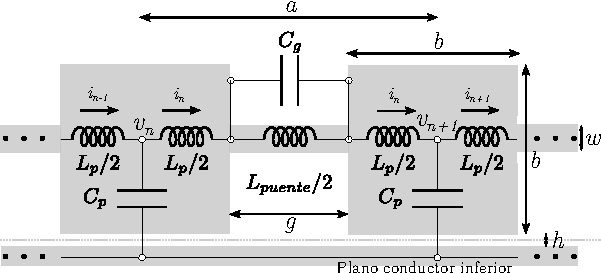
\includegraphics[width=0.9\textwidth]{Fundamentos/circuito-equivalente-celda-unitaria.pdf}
	\caption{Circuito equivalente propuesto para el análisis de primer modo de una celda unitaria bidimensional arbitraria, propuesto por \cite{KimSchuttAine:AnalysisHybrid}.}
	\label{fig:circuito-equivalente-kim-parches}
\end{figure}

%\begin{figure}[htp]
%	\centering
%	\begin{circuitikz} \draw
%		(0,0) -- (1,0)node[midway,scale=2,fill=white]{$\cdots$}
%		-- (9,0) -- (10,0)node[midway,scale=2,fill=white]{$\cdots$}
%		(0,2) -- (1,2)node[midway,scale=2,fill=white]{$\cdots$} 
%		to [L,-o,l_=$L_p/2$] (2.5,2)
%		to [L,o-o,l_=$L_p/2$] (4,2)
%		to [L,o-o,l_=$L_{puente}/2$] (6,2)
%		to [L,o-o,l_=$L_p/2$] (7.5,2)
%		to [L,o-,l_=$L_p/2$] (9,2)
%		-- (10,2)node[midway,scale=2,fill=white]{$\cdots$}
%		(2.5,2) to [C,o-o,l_=$C_p$] (2.5,0)
%		(7.5,2) to [C,o-o,l_=$C_p$] (7.5,0)
%		(4,3) to [C,o-o,l^=$C_g$] (6,3);
%		%			to [C,l=$C'_R \Delta_z$] (7,0)
%		%		-- (9,0) to [L,l_=$L'_L / \Delta_z$] (9,2)
%		%		-- (7,2)
%		%		(9,2) -- (11,2)
%		%		to [R,l=$R / \Delta_z$] (11,0)
%		%		-- (9,0)
%		%		(11,0) -- (12,0) -- (13,0)node[midway,scale=2,fill=white]{$\cdots$}
%		%		(11,2) -- (12,2) -- (13,2)node[midway,scale=2,fill=white]{$\cdots$};
%	\end{circuitikz}  	
%	\caption{Circuito equivalente de porción de línea de transmisión cargada, de longitud $d$.}
%	\label{fig:linea-transm-cargada-periodica}
%\end{figure}


El análisis de la expresión de dispersión no se puede realizar utilizando el acercamiento circuital propuesto, debido a que cada nodo del circuito posee una fase establecida por los parámetros concentrados.

Si bien existen múltiples procedimientos posibles para lograr una expresión de dispersión, en este trabajo se analizarán solo dos para la estructura de la figura \ref{fig:circuito-equivalente-kim-parches}: la explicada en la sección \ref{sec:diag-de-dispersion}, y una evaluación en base al planteo de líneas de transmisión generalizadas, utilizando los conceptos desarrollados en la sección \ref{sec_lineas_de_transmision}.

El primer método requiere que se divida a cada celda unitaria en trozos de línea de transmisión de impedancias diferentes, en función de su ancho, como se muestra en la figura \ref{fig:division_en_trozos_impedancia}.

Para el caso unidimensional, si se intentara obtener una expresión de la ecuación de dispersión utilizando un acercamiento circuital de parámetros concentrados, , considerando el circuito de la figura \ref{fig:circuito-equivalente-kim-parches}, donde se demarcaron las tensiones y corrientes a considerar, alrededor de una celda unitaria determinada ($n$). A partir del planteo de las ecuaciones circuitales, y considerando que las tensiones y corrientes tienen un comportamiento armónico:

\begin{align}
	v_n - v_{n+1} = i_n \left( j \omega \frac{L_p}{2} + \frac{j \omega L_b}{1-\omega^2 L_b C_g} + j \omega \frac{L_p}{2} \right) \\
	\frac{i_n - i_{n+1}}{j\omega C_p} = v_n
\end{align}

Reordenando e imponiendo la condición de Bloch-Floquet, que indica, expresado de forma conveniente, que $i_{n+1} = i_{n} e^{-\gamma a}$, y que $v_{n+1} = v_{n} e^{-\gamma a}$:

\begin{align}
	\begin{bmatrix}
		1 & -j \omega C_p \\
		-\frac{L_p}{2} - \frac{j \omega L_b}{1-\omega^2 L_b C_g} - \frac{L_p}{2} & 1
	\end{bmatrix}
	\begin{bmatrix}
		i_n \\
		v_n
	\end{bmatrix}
	=
	\begin{bmatrix}
		i_{n+1} \\
		v_{n+1}
	\end{bmatrix}
	=
	\begin{bmatrix}
		i_n e^{-j\gamma a} \\
		v_n e^{-j\gamma a}
	\end{bmatrix}
	=
	\begin{bmatrix}
		1 & 0 \\
		0 & 1
	\end{bmatrix}
	\begin{bmatrix}
		i_n e^{-j\gamma a} \\
		v_n e^{-j\gamma a}
	\end{bmatrix}
\end{align}

Lo que se reduce a:

\begin{align}
	\begin{bmatrix}
		1-e^{-j\gamma a} & -j \omega C_p \\
		-\frac{L_p}{2} - \frac{j \omega L_b}{1-\omega^2 L_b C_g} - \frac{L_p}{2} & 1-e^{-j\gamma a}
	\end{bmatrix}
	\begin{bmatrix}
		i_n \\
		v_n
	\end{bmatrix}
	=0
\end{align}

Para obtener soluciones más allá de la trivial, el determinante de la matriz debe ser cero, por lo que resulta la ecuación de dispersión:

\begin{align}
	\label{eq:dispersion-teorica}
	1+e^{-2j\gamma a} - 2 e^{-j\gamma a} - j \omega C_p L_p + \frac{\omega^2 C_p L_b}{1-\omega^2 L_b C_g} = 0.
\end{align}

Cuando $\gamma$ es puramente imaginario (es decir, $\alpha = 0$, y por tanto, $\gamma=-j\beta$), la onda se propaga libremente. Cuando $\beta = 0$, $\gamma$ es puramente real y la onda no viaja sobre la superficie, sino que, por el contrario, manifiesta un comportamiento evanescente.

La expresión \ref{eq:dispersion-teorica} se puede reformular, utilizando la fórmula de Euler, para obtener las ecuaciones para la parte real y la parte imaginaria por separado.

Si se considera únicamente la parte imaginaria, resulta

\begin{align}
\label{eq:ec-dispersion-imag}
-e^{-2\alpha a} \sin(2j\beta a) + j 2e^{-\alpha a} \sin(j\beta a) = j \omega C_p L_p,
\end{align}

cuya gráfica se observa en la figura \ref{fig:ec-dispersion-imag}, para los valores circuitales y geométricos expresados en la tabla \ref{table:diag-disp-teorico}. En la misma se observa que, para las frecuencias de interés, no existen limitaciones: Cualquiera sea la frecuencia de trabajo, existirá algún $\beta$ que, según la expresión para la parte imaginaria analizada, permita la propagación de ondas sobre la superficie. Se debe tener en cuenta que ambas expresiones (la asociada a la parte real y la correspondiente a la parte imaginaria) deben cumplirse.

\begin{figure}[h]
	\centering
	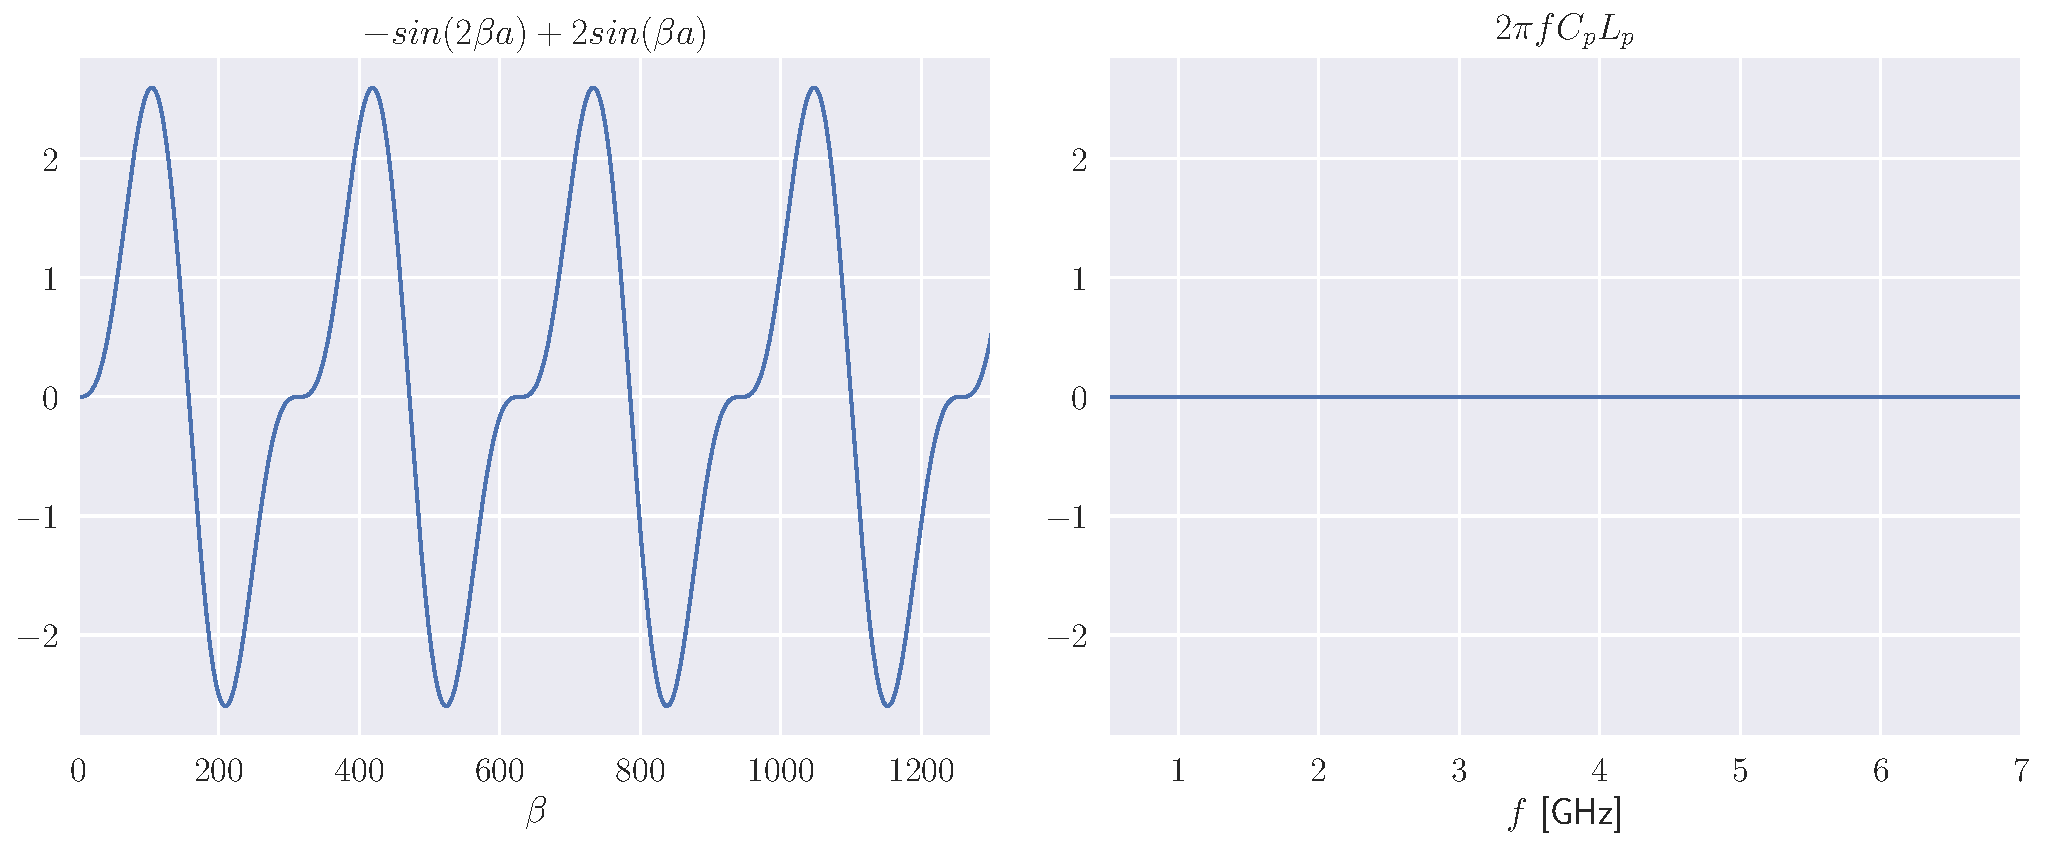
\includegraphics[width=1\textwidth]{Modelado/subplots-diagdisp-imag.pdf}
	\caption{Gráficas de la expresión \ref{eq:ec-dispersion-imag}.}
	\label{fig:ec-dispersion-imag}
\end{figure}

\begin{table}
	\centering
	\begin{tabular}{| c c | c c | c c | c c |} 
		$g$ & $4\; mm$ & $ag$ & $20\; mm$ & $b$ & $17\; mm$ & $w$ & $1\; mm$\\
		\hline
		$C_p$ & $7\; pF$ & $L_p$ & $2\; nH$ & $C_g$ & $731\; fF$ & $L_b$ & $1.85\; nH$\\
	\end{tabular}
	\caption{Tabla de valores finales elegidos.}
	\label{table:valoresFinalesModelo}
\end{table}


De la misma manera, la expresión para la parte imaginaria resulta

\begin{align}
	\label{eq:ec-dispersion-real}
	1+e^{-2\alpha a} \cos(2j\beta a) - 2e^{-\alpha a} \cos(j\beta a) = -\frac{\omega^2 L_b C_p}{1-\omega^2 L_b C_g},
\end{align}

cuyas gráficas, para ambas expresiones a cada lado del igual, se muestran en la figura \ref{fig:ec-dispersion-real} para $\alpha = 0$. Resulta importante notar que, bajo la restricción de pérdidas nulas, valores de frecuencia por encima de aproximadamente $0.7\; GHz$ no son realizables, pues no existe valor de $\beta$ que permita que el lado izquierdo de la ecuación \ref{eq:ec-dispersion-real} resulte menor a -0.5. Para cualquier frecuencia de fuente menor a dicho valor, existirá al menos un $\beta$ que asegure su propagación.

Por encima de dicha frecuencia, no existirá propagación pura. Si se consideraran pérdidas ($\alpha>0$), los cosenos graficados estarían afectados por el producto con exponenciales negativas, por lo que la amplitud de los cosenos de la gráfica izquierda de la figura \ref{fig:ec-dispersion-real} disminuiría, aumentando aún más la zona de frecuencias prohibidas, volviendo el valor umbral menor a $0.7\; GHz$.

Resulta necesario aclarar, sin embargo, que en el circuito propuesto se puede observar únicamente el comportamiento de los modos cuasi-TEM sobre las celdas unitarias de la estructura periódica, pues es a partir de los mismos que se obtienen las expresiones y disposiciones de capacidades e inductancias utilizadas en el modelo. Esto significa que existirán modos superiores, pero que no pueden ser predichos por el modelo cuasiestático planteado.

\begin{figure}[h]
	\centering
	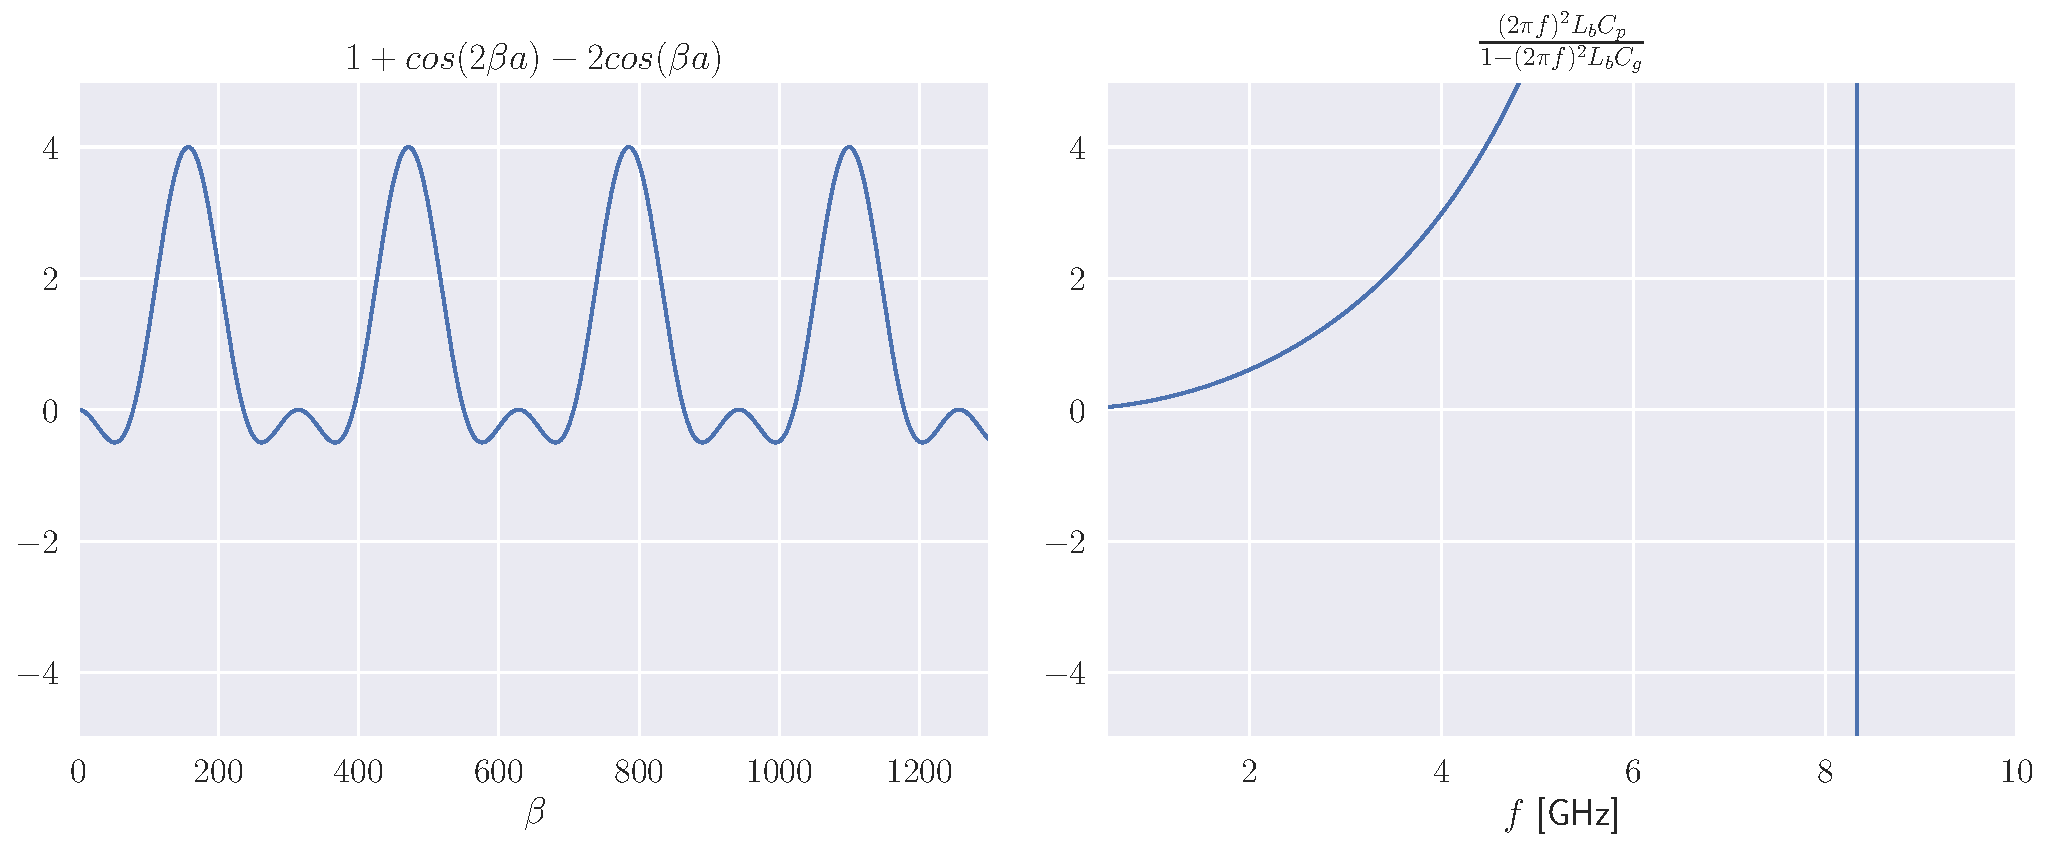
\includegraphics[width=1\textwidth]{Modelado/subplots-diagdisp-real.pdf}
	\caption{Gráficas de la expresión \ref{eq:ec-dispersion-real}.}
	\label{fig:ec-dispersion-real}
\end{figure}






Para el caso de las superficies de alta impedancia sin vías de conexión entre la geometría superior y el plano de tierra inferior, Tretyakov y otros (\cite{Tretyakov:AnalyticalModeling}, \cite{Yakovlev:AnalyticalModelingHIS}) han propuesto un análisis centrado en la similitud con las FSS (\textit{Frequency Selective Surfaces}), considerando a las superficies EBG uniplanares como FSS con un plano de tierra. De esta manera es posible utilizar los modelos desarrollados durante el siglo \textsc{XX} para el análisis de las superficies selectoras de frecuencias, en el estudio de EBGs, dado que el comportamiento de banda prohibida se da por el mismo motivo que el comportamiento de filtro de las FSS \cite{Goussetis:TailoringAMCEBGCharacteristics}, relacionado a la frecuencia de resonancia del arreglo de elementos. Para ello, se considera el circuito equivalente de la figura \ref{fig:tretyankov-circuito-equivalente}, donde $Z_g$ es la impedancia que impone la FSS que se dispone sobre el plano dieléctrico, y $Z_d$ es la impedancia del conjunto formado por el dieléctrico y el plano conductor. De esta forma, la impedancia de superficie resulta del paralelo de ambas. La impedancia del conjunto dieléctrico-plano conductor fue analizada en el capítulo anterior, y depende de la polarización (TE o TM). La impedancia que impone el arreglo periódico bidimensional, la FSS, requiere de un análisis particular de cada caso, y los resultados analíticos en la literatura están limitados a arreglos de rectángulos, dipolos y cruces, y sus correspondientes estructuras complementarias.

\begin{figure}
	\centering
	\begin{circuitikz} \draw
		(0,2) to[transmission line, o-o,l=$Z_0$] (3,2)
		to[generic, o-o,l=$Z_g$] (3,4)
		(0,4) to[transmission line, o-o] (3,4)
		(3,2) -- (5,2)
		to[generic,o-o,l=$Z_d$] (5,4)
		-- (3,4);
	\end{circuitikz}
	\caption{Circuito equivalente propuesto por \cite{Yakovlev:AnalyticalModelingHIS} para un EBG.}
	\label{fig:tretyankov-circuito-equivalente}
\end{figure}

Un planteo intuitivo de los resultados de Tretyankov requiere comenzar el análisis a partir del conocimiento de que, como se demostró en la sección \ref{sec:ondas-de-superficie}, y como se muestra en la figura \ref{fig:beta-reactancia-TM}, una superficie con impedancia inductiva es capaz de soportar ondas TM. La impedancia de un plano de tierra recubierto por un material dieléctrico, $Z_d$, como se muestra en la ecuación \ref{eq:impedancia-superficie-tm-teorica}, resulta inductiva. Para lograr una impedancia superficial $Z_s$ menos inductiva, en vistas de disminuir el comportamiento de guía de ondas de la estructura, se debe imponer una impedancia $Z_g$ acorde.

El metamaterial basado en FSS más usual, el arreglo de parches, da lugar a una impedancia $Z_g$ capacitiva, tanto por la capacidad impuesta entre los parches y el plano de tierra, como por la capacidad entre los parches adyacentes. Para frecuencias bajas, el comportamiento del circuito equivalente es inductivo, pero para frecuencias por encima de la de resonancia, el comportamiento es capacitivo. Por otro lado, es posible considerar, si los parches son lo suficientemente grandes, que los mismos presentan una inductancia, en serie con las capacidades parásitas descriptas antes. Un inductor en paralelo con el inductor correspondiente al plano conductor de la cara inferior del dieléctrico disminuye la inductancia total, por lo que se logra el efecto deseado. Finalmente, si los parches son conectados, como se mostró en la figura \ref{fig:circuito-equivalente-kim-parches}, la inductancia en paralelo con la capacidad entre parches acrecentará este efecto. Los efectos que se presentan por encima de la frecuencia de resonancia impiden que el análisis intuitivo describa la existencia de modos superiores, por lo que estas consideraciones no son completas, lo que obliga a que la frecuencia de resonancia no esté muy por debajo de la frecuencia de ondas de superficie que se desea bloquear con la estructura EBG.

\section{Técnicas numéricas de onda completa}
\label{sec_estructuras_periodicas}
%%%%
% Libro de rahmat. Pagina 59.
%%%%

El análisis mediante circuitos equivalentes sólo permite el modelado de efectos de primer orden y, en general, en sólo dos dimensiones. El uso de herramientas tridimensionales de cálculo numérico permite observar los efectos de orden superior, así como evaluar los campos radiados por la estructura y los posibles efectos de campo cercano \cite{Mohajer:SupressionBand}.

Las técnicas de simulación de onda completa son aquellas en las que se resuelven las ecuaciones de Maxwell (ecuaciones \ref{eq:Maxwell}) sin simplificaciones, por lo que los campos solución son, en general, variables en el tiempo y dependientes de la frecuencia, y el cálculo es más lento que en los métodos simplificados. Requieren del establecimiento de condiciones de borde, y permiten conocer el comportamiento de estructuras arbitrarias.

La solución de las ecuaciones diferenciales vectoriales en el espacio y el tiempo se pueden realizar utilizando distintas técnicas, entre las que destacan el método de momentos (MOM), el método de elementos finitos (FEM) y el método de diferencias finitas en el dominio del tiempo (FDTD).

\begin{itemize}
	\item Método de elementos finitos (FEM): Tiene su origen en el análisis estructural, y desde su primer aplicación al electromagnétismo, en 1968, se convirtió en uno de los métodos diferenciales más importantes. Consiste en dividir en recinto en un número finito de regiones o elementos pequeños (habitualmente triángulos), deducir las ecuaciones que describen los campos dentro de un elemento cualquiera (habitualmente utilizando polinomios de orden $n$), plantear las ecuaciones que dan las condiciones de ajuste de las soluciones en las superficies frontera (en general, agregando como requisito que la solución sea la de mínima energía) y, finalmente, resolver el sistema de ecuaciones lineales resultante \cite{Fernandez:Electromag}. Debido a que se debe discretizar el espacio completo sobre el que se realizará la simulación, la cantidad de incógnitas es proporcional al volumen y la resolución considerada, aunque no de la complejidad de la estructura simulada, de modo que resulta especialmente útil en aplicaciones pequeñas y complejas (con inhomogeneidades). Para solventar el problema de la simulación de volúmenes abiertos, han surgido diversas estrategias, entre las que destaca el uso de \textit{Absorbing Boundary Conditions} (ABC) y \textit{Perfectly Matches Layers} (PML) en los límites del dominio de cálculo para simular espacio abierto. Su implementación más conocida está incluida en el programa Ansoft HFSS.
	\item Método de momentos (MOM): Se suele utilizar para el cálculo de estructuras radiantes, debido a que es un método de resolución de ecuaciones integrales, donde se formula el problema del campo electromagnético en términos de corrientes desconocidas que circulan por los objetos modelados. Estas corrientes se acoplan a través de las funciones tensoriales de Green, y tienen en cuenta automáticamente el espacio circundante. Para esto se debe establecer el operador lineal, para luego resolver un sistema de ecuaciones operacionales lineales relacionadas con el conjunto de las corrientes que circulan sobre los conductores, donde la función solución (los campos que se desea hallar) se representan como un desarrollo en serie de funciones base a las que se aplica el operador, y donde las incógnitas son los coeficientes constantes utilizados en el desarrollo en serie de la función resultado. Es un método en el dominio de la frecuencia, y sus implementaciones más conocida son las usadas por el software NEC-2 \cite{Fernandez:Electromag}, Keysight Advanced Design Systems (ADS) y FEKO.
	\item Método de diferencias finitas en el dominio del tiempo (FDTD): Consiste en la discretización en el espacio y el tiempo, mediante las denominadas celdas de Yee, que permiten el uso de la técnica numérica de salto de rana: Dado que las derivadas temporales de cada uno de los campos dependen del rotor del otro, los campos eléctrico y magnético se evalúan en puntos alternados (en la mitad de los puntos se evalúa únicamente el campo eléctrico, y en la otra mitad, campo magnético), de forma que cada punto donde se evalúa campo eléctrico quede rodeado de cuatro componentes donde se calcula campo magnético, y viceversa. La evaluación en el tiempo es también alternada: los campos magnéticos se obtienen $\Delta t/2$ más tarde que los campos eléctricos, de forma que resulte fácil calcular las derivadas en el tiempo y el espacio mediante diferencias finitas. Dado que la solución se obtiene en el dominio del tiempo, este método resulta útil para aplicaciones de banda ancha. El software comercial más conocido que aplica está técnica es CST Microwave Studio.
\end{itemize}

Para el caso particular del FDTD, es posible resolver problemas de autovalores (particularmente, el analizado en la sección \ref{sec:automodos}), útiles en la descripción de guías de onda y metamateriales periódicos. Una vez impuesta una excitación en el tiempo $t=0$, los valores de campos se actualizan tiempo a tiempo para todos los puntos del dominio de cálculo de forma iterativa, hasta que se logra una señal resonante estable.

Para el caso del estudio de cavidades y guías de ondas, las condiciones de borde para el análisis de autovalores suelen ser conductores eléctricos, con o sin pérdidas. Cuando se analizan estructuras periódicas, es común utilizar condiciones de borde periódicas (PBC, \textit{periodic boundary conditions}), que modelan el efecto de replicación periódica, de manera que es posible simular una única celda unitaria para obtener el efecto del metamaterial completo en base a su diagrama de dispersión \cite{Yang:EBGAntennas}, utilizando la disposición mostrada en la figura \ref{fig:esquema-simulacion-periodica}.

\begin{figure}[h]
	\centering
	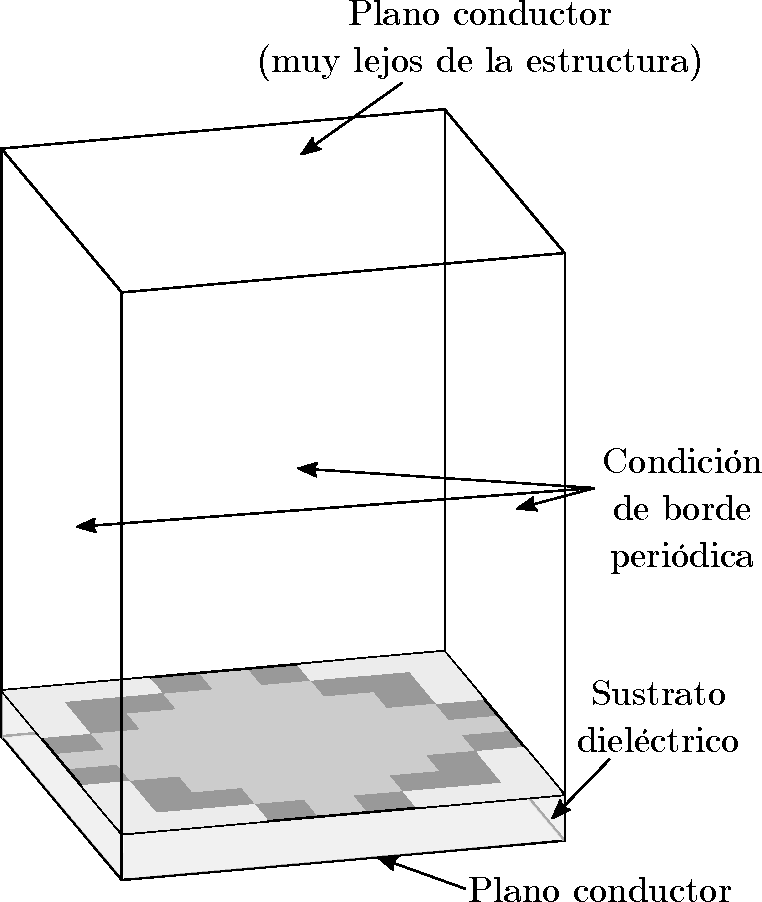
\includegraphics[width=0.6\textwidth]{Modelado/esquema-simulacion-periodica.pdf}
	\caption{Dominio de simulación de una celda unitaria de un metamaterial bidimensional, utilizando condiciones de borde periódicas.}
	\label{fig:esquema-simulacion-periodica}
\end{figure}

El uso de estas condiciones de borde periódicas deriva del teorema de Bloch-Floquet, tratado en la sección \ref{sec:bloch-floquet}. Como se muestra en la ecuación \ref{eq:comportamiento-periodico-campo-bloch}, el campo eléctrico (o magnético) resulta periódico, con la misma periodicidad que el material, a excepción de una variación de fase, dada por el valor de la constante de propagación $\beta$ del medio.

Para obtener el diagrama de dispersión, cada frecuencia $\omega$ debe estar asociada a una o más constantes de propagación de onda $\beta$. O, dicho de otra forma, dada una constante de propagación $\beta$, es necesario encontrar las autofrecuencias asociadas. Fijar el valor de la constante de propagación $\beta$, según la ecuación \ref{eq:comportamiento-periodico-campo-bloch}, equivale a establecer la diferencia de fase entre las paredes opuestas de la celda unitaria ($e^{-j\beta d}$). Una simulación del comportamiento en el tiempo, y una posterior transformada de Fourier para obtener el comportamiento en frecuencia, permite observar picos de amplitud de campo para algunas frecuencias en particular, que son las que autofrecuencias del problema. Dado que la misma diferencia de fase se puede obtener para frecuencias mayores (un ciclo más tarde), se presentará más de un modo.

Como se observó en la sección \ref{sec:diag-de-dispersion}, para la descripción del comportamiento de la relación de dispersión sólo es necesario el cálculo en la denominada zona irreducible de Brillouin, dado que a partir de reflexiones y transposiciones de la misma es posible reconstruir la celda unitaria en el espacio recíproco. Para el caso de celdas unitarias en que hay simetría sobre los ejes $x$ e $y$, y además hay simetría diagonal, la zona irreducible es un triángulo, como se mostró en la figura \ref{fig:rectangulo-cuadrado}.

De esta forma, únicamente hay que fijar, como condiciones de borde, diferencias de fase que se correspondan, entre los distintos puntos que forman una celda de Wignet-Seitz y que se corresponden a la zona irreducible de Brillouin.

% Fullwave: Baccarelli, Paulotto, impreso.
% Hacer estudio gráfico similar al CALOZ, pag 176.


\section{Análisis de campos y modos para distintas estructuras}
\label{sec_estructuras_propuestas}

\subsection{Metamaterial formado por parches cuadrados unidos por finas trazas \textit{microstrip}}
\label{sec:celdas-orlandi}

Uno de los metamateriales más fáciles de construir, y que en general presenta buenos resultados al mismo tiempo que mantiene una geometría sencilla es el que se observa en la figura \ref{fig:celda-orlandi}. En la misma, $d$ es el lado de la celda unitaria (cuadrada), $l$ es el tamaño del lado del cuadrado metálico (de cobre), y $l_m$ y $w_m$ son el largo y el ancho de los puentes que comunican a los parches, respectivamente.

\begin{figure}[h]
	\centering
	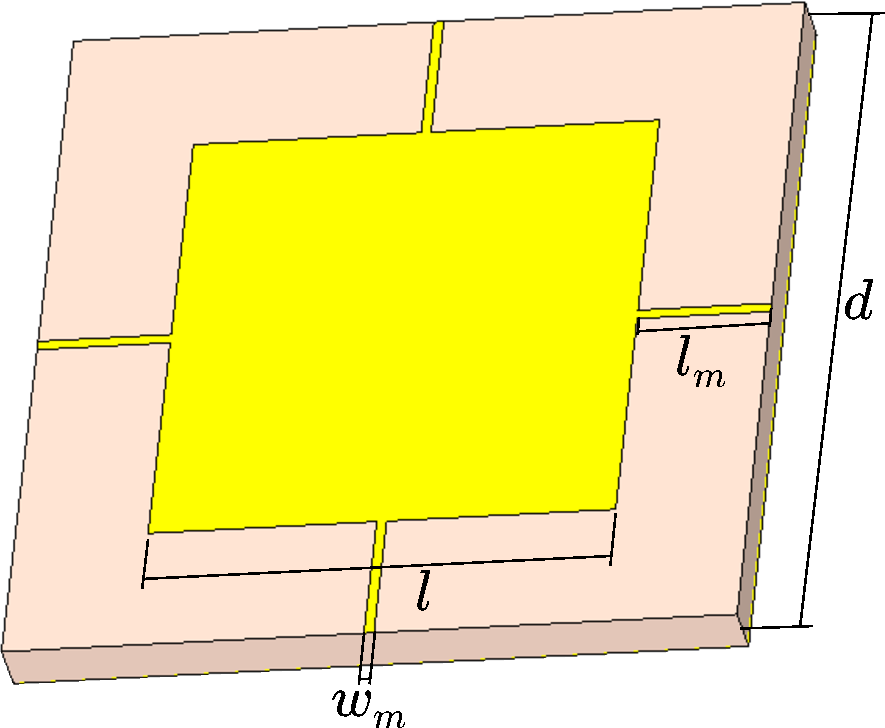
\includegraphics[width=0.4\textwidth]{Modelado/orlandi-celda.pdf}
	\caption{Celda unitaria de un metamaterial formado por parches cuadrados unidos por finas trazas \textit{microstrip}.}
	\label{fig:celda-orlandi}
\end{figure}

Esta geometría resulta sencilla de analizar, debido principalmente a que, como se estudió en la sección \ref{sec:modelo_analitico}, cada aspecto de la misma tiene un equivalente circuital, al menos para las frecuencias más bajas, que varía en función de los parámetros constructivos. La celda unidad propuesta posee una simetría tal que permite realizar un análisis en una zona de Brillouin triangular, como la que se mostró, teóricamente, en la figura \ref{fig:explicacion-zona-brillouin}.

Aplicando el análisis de autovalores explicado en la sección precedente, es posible obtener, para cada condición de borde periódica en que va variando la fase de las paredes opuestas que conforman el contorno condicionado, un conjunto de frecuencias que representan los modos de propagación en cada dirección analizada, lo que permite crear un diagrama de dispersión, similar al mostrado en la figura \ref{fig:diagrama-dispersion-vacio-2d}, aunque con modos superiores.

\begin{figure}[h]
	\centering
	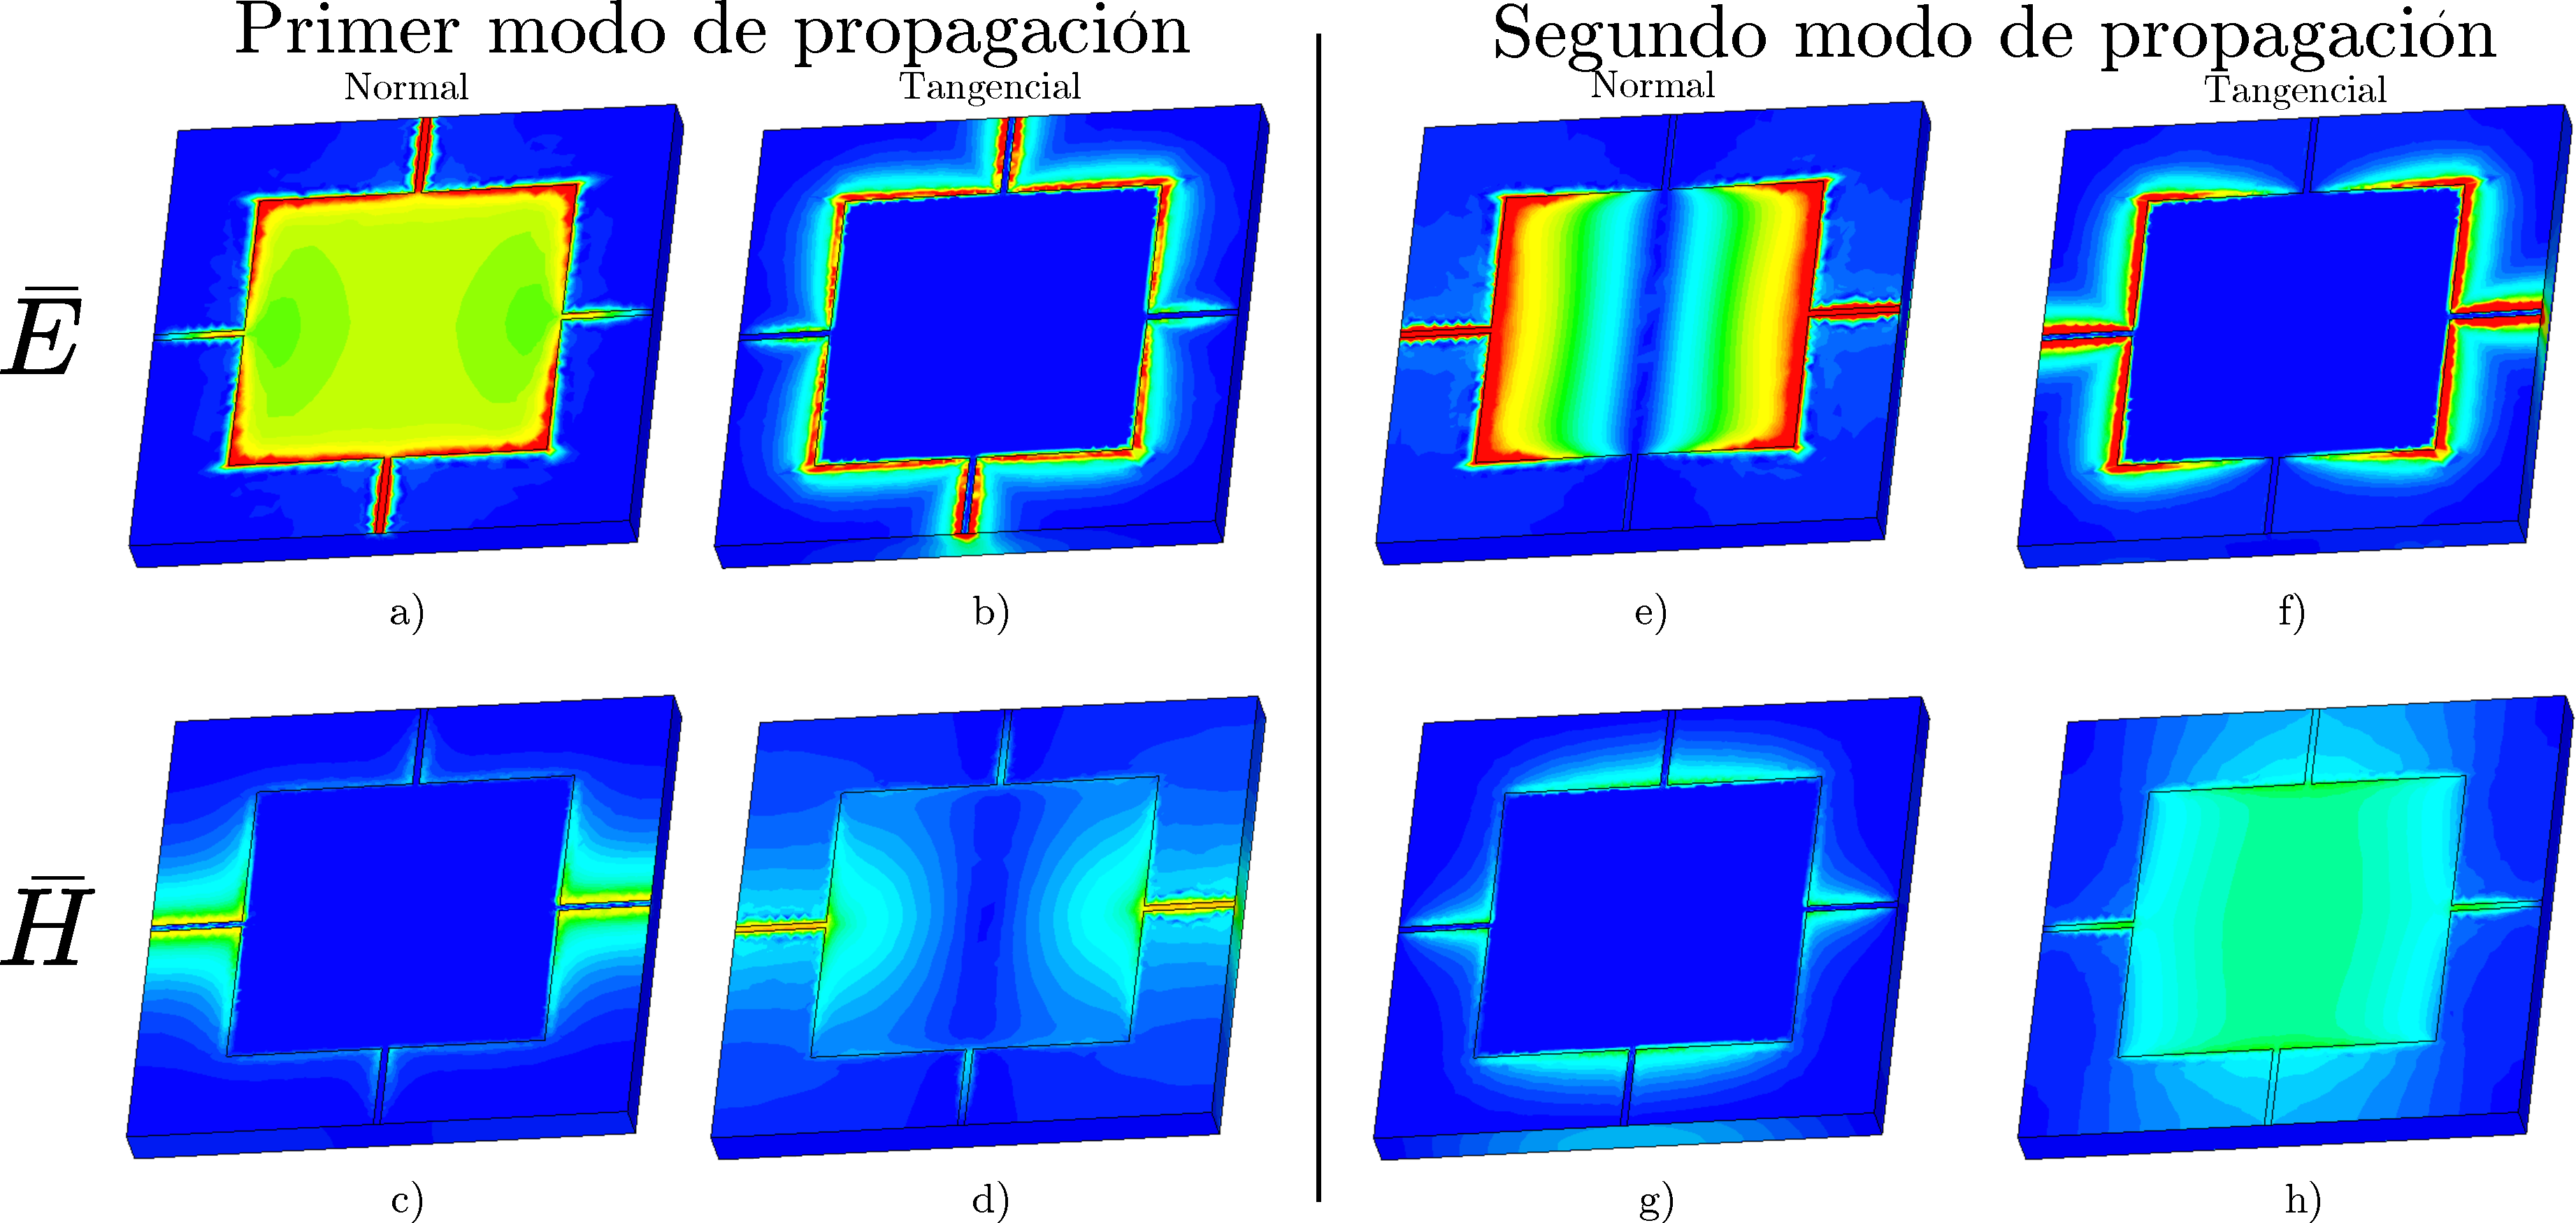
\includegraphics[width=1\textwidth]{Modelado/orlandi-modo1-Enorma-Etangencial.pdf}
	\caption{Comportamiento, en promedio temporal, de los campos eléctrico y magnético sobre una celda unitaria formada por un parche central y 4 puentes laterales, para el primer y segundo modo de propagación.}
	\label{fig:orlandi-analisis-campos}
\end{figure}

En la figura \ref{fig:orlandi-analisis-campos} se ilustran\footnote{Debido a la naturaleza de la simuación con autovalores, que no impone una tensión inicial, los valores obtenidos de los campos no son representativos de la situación física (aunque sí la morfología espacial). Estos valores obtenidos, no mostrados en la figura, suelen ser altos debido al mecanismo de simulación. El análisis que se pretende realizar aquí del comportamiento de los campos es puramente conceptual.}, para los dos primeros modos de propagación, los campos eléctrico y magnético en dirección normal y tangencial a la superficie, considerando una dirección de propagación horizontal (equivalente al punto $M$ en la figura \ref{fig:explicacion-zona-brillouin}).

En la figura \ref{fig:orlandi-analisis-campos} a) se muestra el comportamiento del campo eléctrico promedio perpendicular a la superficie para el primer modo de propagación. Resulta claro que el mismo se concentra debajo del parche metálico que conforma a la celda unitaria, debido a que la presencia de un plano de tierra genera un comportamiento de planas planas paralelas, conformando efectivamente un capacitor. Es también notoria la presencia de campo eléctrico en dirección normal a la superficie en los puentes \textit{microstrip} superior e inferior, debido principalmente a que no hay movimiento de cargas en dirección longitudinal a los mismos, sino que actúan como extensiones al parche central, aumentando ligeramente la capacidad del dispositivo.

El campo eléctrico en la dirección tangencial, también para el primer modo de propagación, es ilustrado en la figura \ref{fig:orlandi-analisis-campos} b), y permite observar la existencia de notorios efectos de \textit{fringing} alrededor de todo el parche, que deben ser considerados en el análisis. Estos efectos son mayores sobre los puentes superior e inferior, nuevamente, mientras que sobre los puentes ubicados horizontalmente parece no haber concentración de cargas. Esto se confirma al analizar las figuras \ref{fig:orlandi-analisis-campos} c) y d), que ilustran el campo magnético en dirección normal y tangencial a la superficie, respectivamente. Se puede observar que no existen campos magnéticos normales a la superficie debajo del parche metálico, sino que, como muestra la figura d), son puramente tangenciales. Debajo del parche, entonces, para el primer modo de propagación, los campos son cuasi-TEM. La presencia de campo magnético sobre los puentes horizontales corrobora la hipótesis de que sobre los mismos se genera corriente, que ingresa al parche metálico para ser conducida.

\begin{figure}[h]
	\centering
	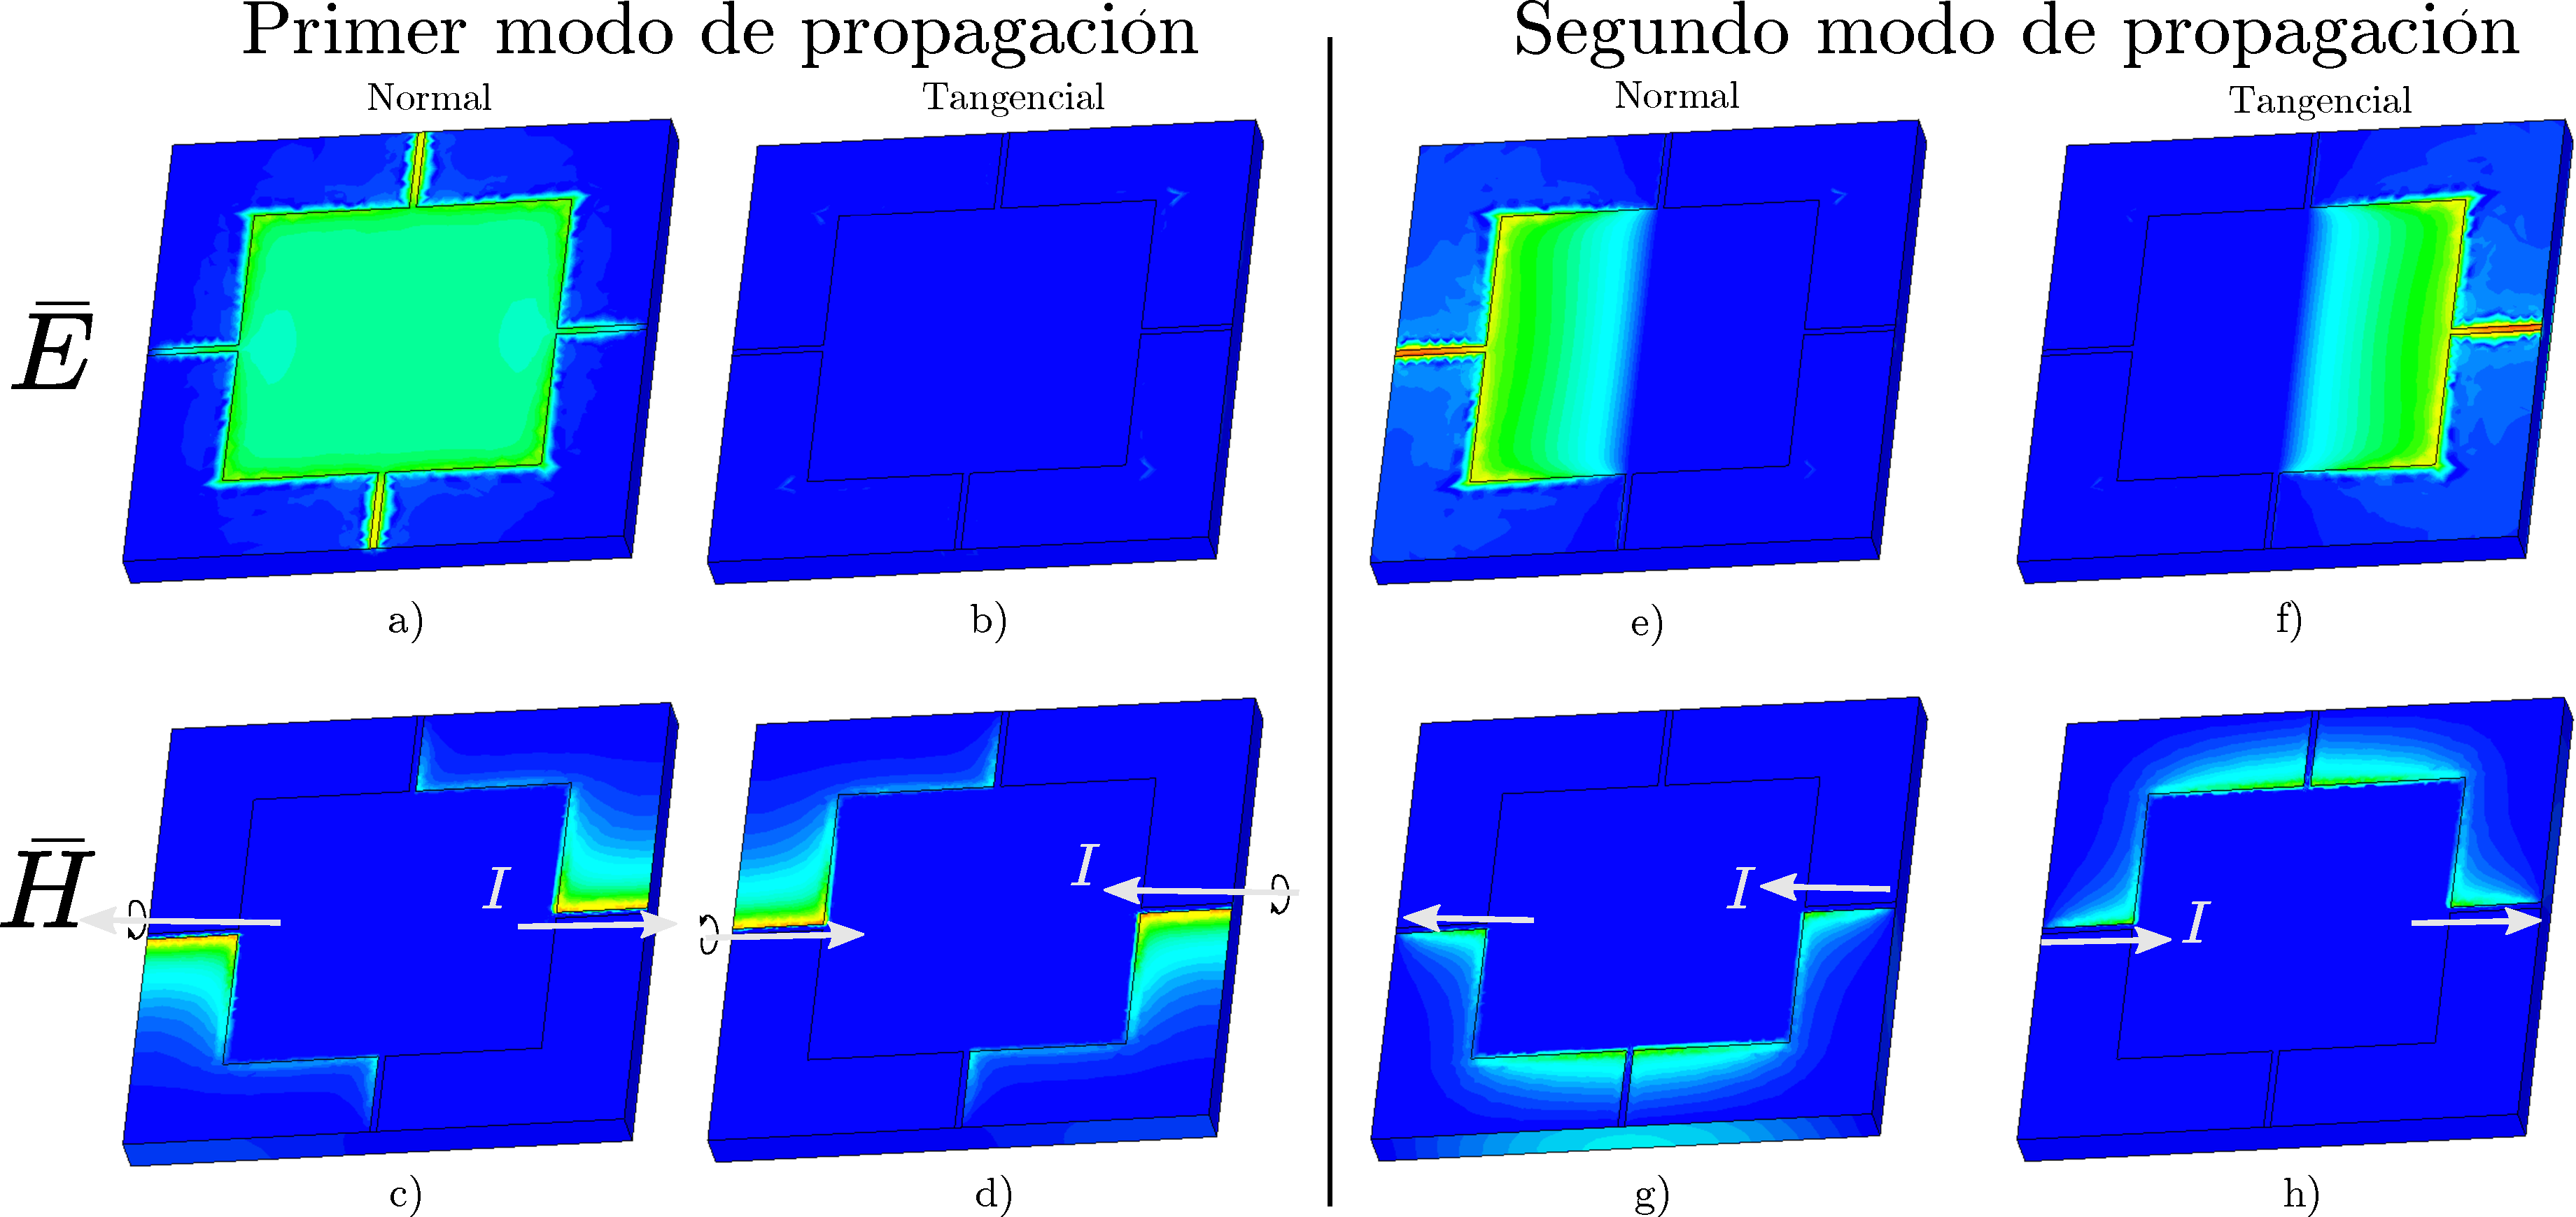
\includegraphics[width=1\textwidth]{Modelado/orlandi-modo1-EH-fases.pdf}
	\caption{Comportamiento, para dos tiempos diferentes, de los campos eléctrico y magnético normales a la superficie, sobre una celda unitaria formada por un parche central y 4 puentes laterales, para el primer y segundo modo de propagación.}
	\label{fig:orlandi-analisis-campos-fases}
\end{figure}

El análisis para el primer modo de propagación continúa en la figura \ref{fig:orlandi-analisis-campos-fases}. En las figuras \ref{fig:orlandi-analisis-campos-fases} a) y b) se muestra el comportamiento del campo eléctrico para dos momentos de tiempo diferentes. Se observa que el parche almacena cargas durante un breve tiempo, y las expele inmediatamente después. Esto se ve corroborado por el comportamiento del campo magnético normal a la superficie, mostrado en escala lineal en las figuras \ref{fig:orlandi-analisis-campos-fases} c) y d), para dos tiempos distintos, y donde se ven colores cuando el campo es positivo en la dirección perpendicular saliente a la superficie del parche. A través del uso de la regla de la mano derecha, se pueden deducir las direcciones de las corrientes sobre los puentes, que son las especificadas por flechas, y donde se observa que son opuestas en el primer modo. Es decir, de forma intuitiva, las corrientes son entrantes al parche de todas direcciones al mismo tiempo, y son salientes del mismo hacia todas direcciones en un tiempo subsiguiente. De esta forma, el parche posee cargas positivas completamente en un tiempo, y luego cargas negativas en el tiempo siguiente, lo cual coincide con la intuición del concepto de un primer modo de propagación, y con el análisis intuitivo detallado.

El segundo modo de propagación, para la misma dirección y posición sobre el diagrama de dispersión (punto "M"), posee un comportamiento más complejo. Como se observa en la figura \ref{fig:orlandi-analisis-campos} e), el campo eléctrico presenta un cero en el centro de la celda unidad, en la figura f) es coherente con esta observación, dado que cerca del centro y de los puentes verticales no hay campo de \textit{fringing}. El campo magnético, por otro lado, mostrado en las figuras g) y h), nuevamente no parece permitir concebir corrientes sobre los puentes verticales, aunque sí en el interior del parche metálico propiamente dicho.

El análisis de dos tiempos diferentes dentro del ciclo para el segundo modo de propagación, mostrado en las figuras \ref{fig:orlandi-analisis-campos-fases} e)-h), permite comprender más intuitivamente el comportamiento. Se observa que el parche central es excitado (posee campo eléctrico vertical) en dos tiempos diferentes, y sólo una de sus mitades lo es cada vez. Hay un desfasaje de $180^\circ$ entre ambos lados del parche. Observando el campo magnético, resula también intuitivo considerar que cuando la mitad izquierda del parche está excitada, es decir, cuando posee cargas almacenadas, formando un capacitor con el plano de tierra, se genera una corriente hacia la celda vecina, que posee un parche con tensión opuesta. En el lado derecho, el efecto es análogo. Es importante notar que, al contrario que en el caso del primer modo, en el segundo modo de propagación las corrientes de los puentes tienen el mismo sentido en cada tiempo.

La figura \ref{fig:dibujito-modos} ilustra, de forma esquemática e informal, el comportamiento de la fase del campo eléctrico para ambos modos de propagación, de manera que se pueda apreciar el requerido aumento de frecuencia para la concreción del segundo modo.

\begin{figure}[h]
	\centering
	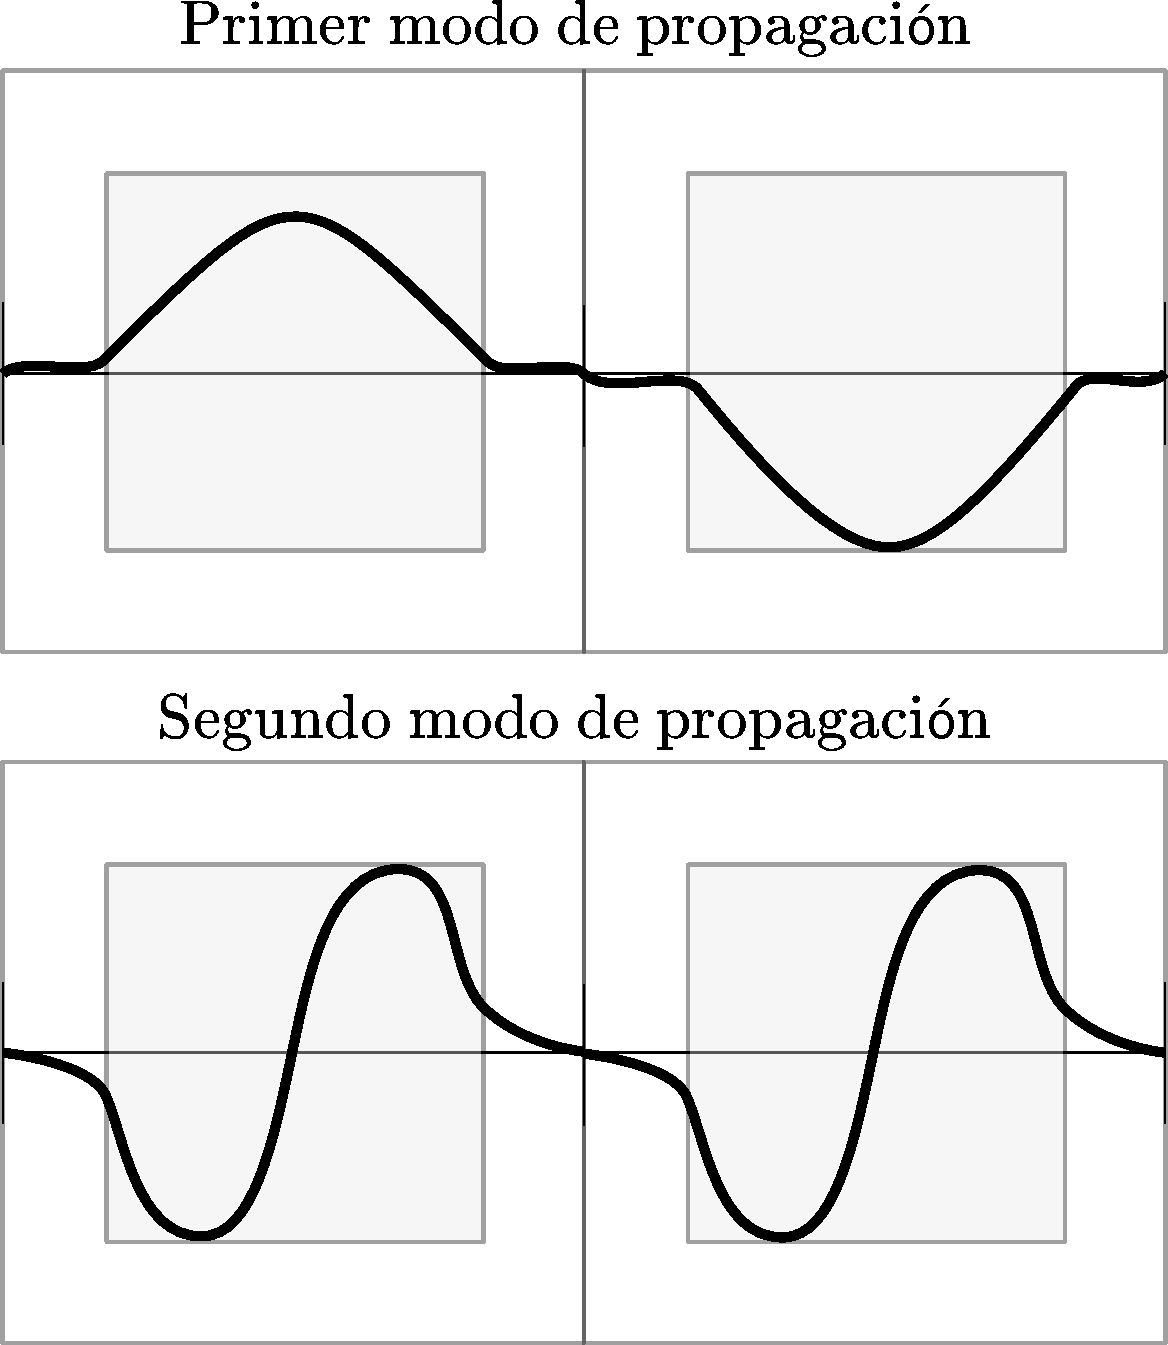
\includegraphics[width=0.4\textwidth]{Modelado/modos-de-propagacion-ilustracion.pdf}
	\caption{Comportamiento, para dos tiempos diferentes, del campo eléctrico sobre una celda unitaria formada por un parche central y 4 puentes laterales, para el primer y segundo modo de propagación.}
	\label{fig:dibujito-modos}
\end{figure}


Para comprender el efecto de la variación de distintos parámetros geométricos, se realizaron varias simulaciones, obteniendo de ellas los diagramas de dispersión.

\subsubsection{Análisis de un diagrama de dispersión típico}

En la figura \ref{fig:diag-dispersion-tipico} se puede observar un diagrama de dispersión típico.

\begin{figure}[h]
	\centering
	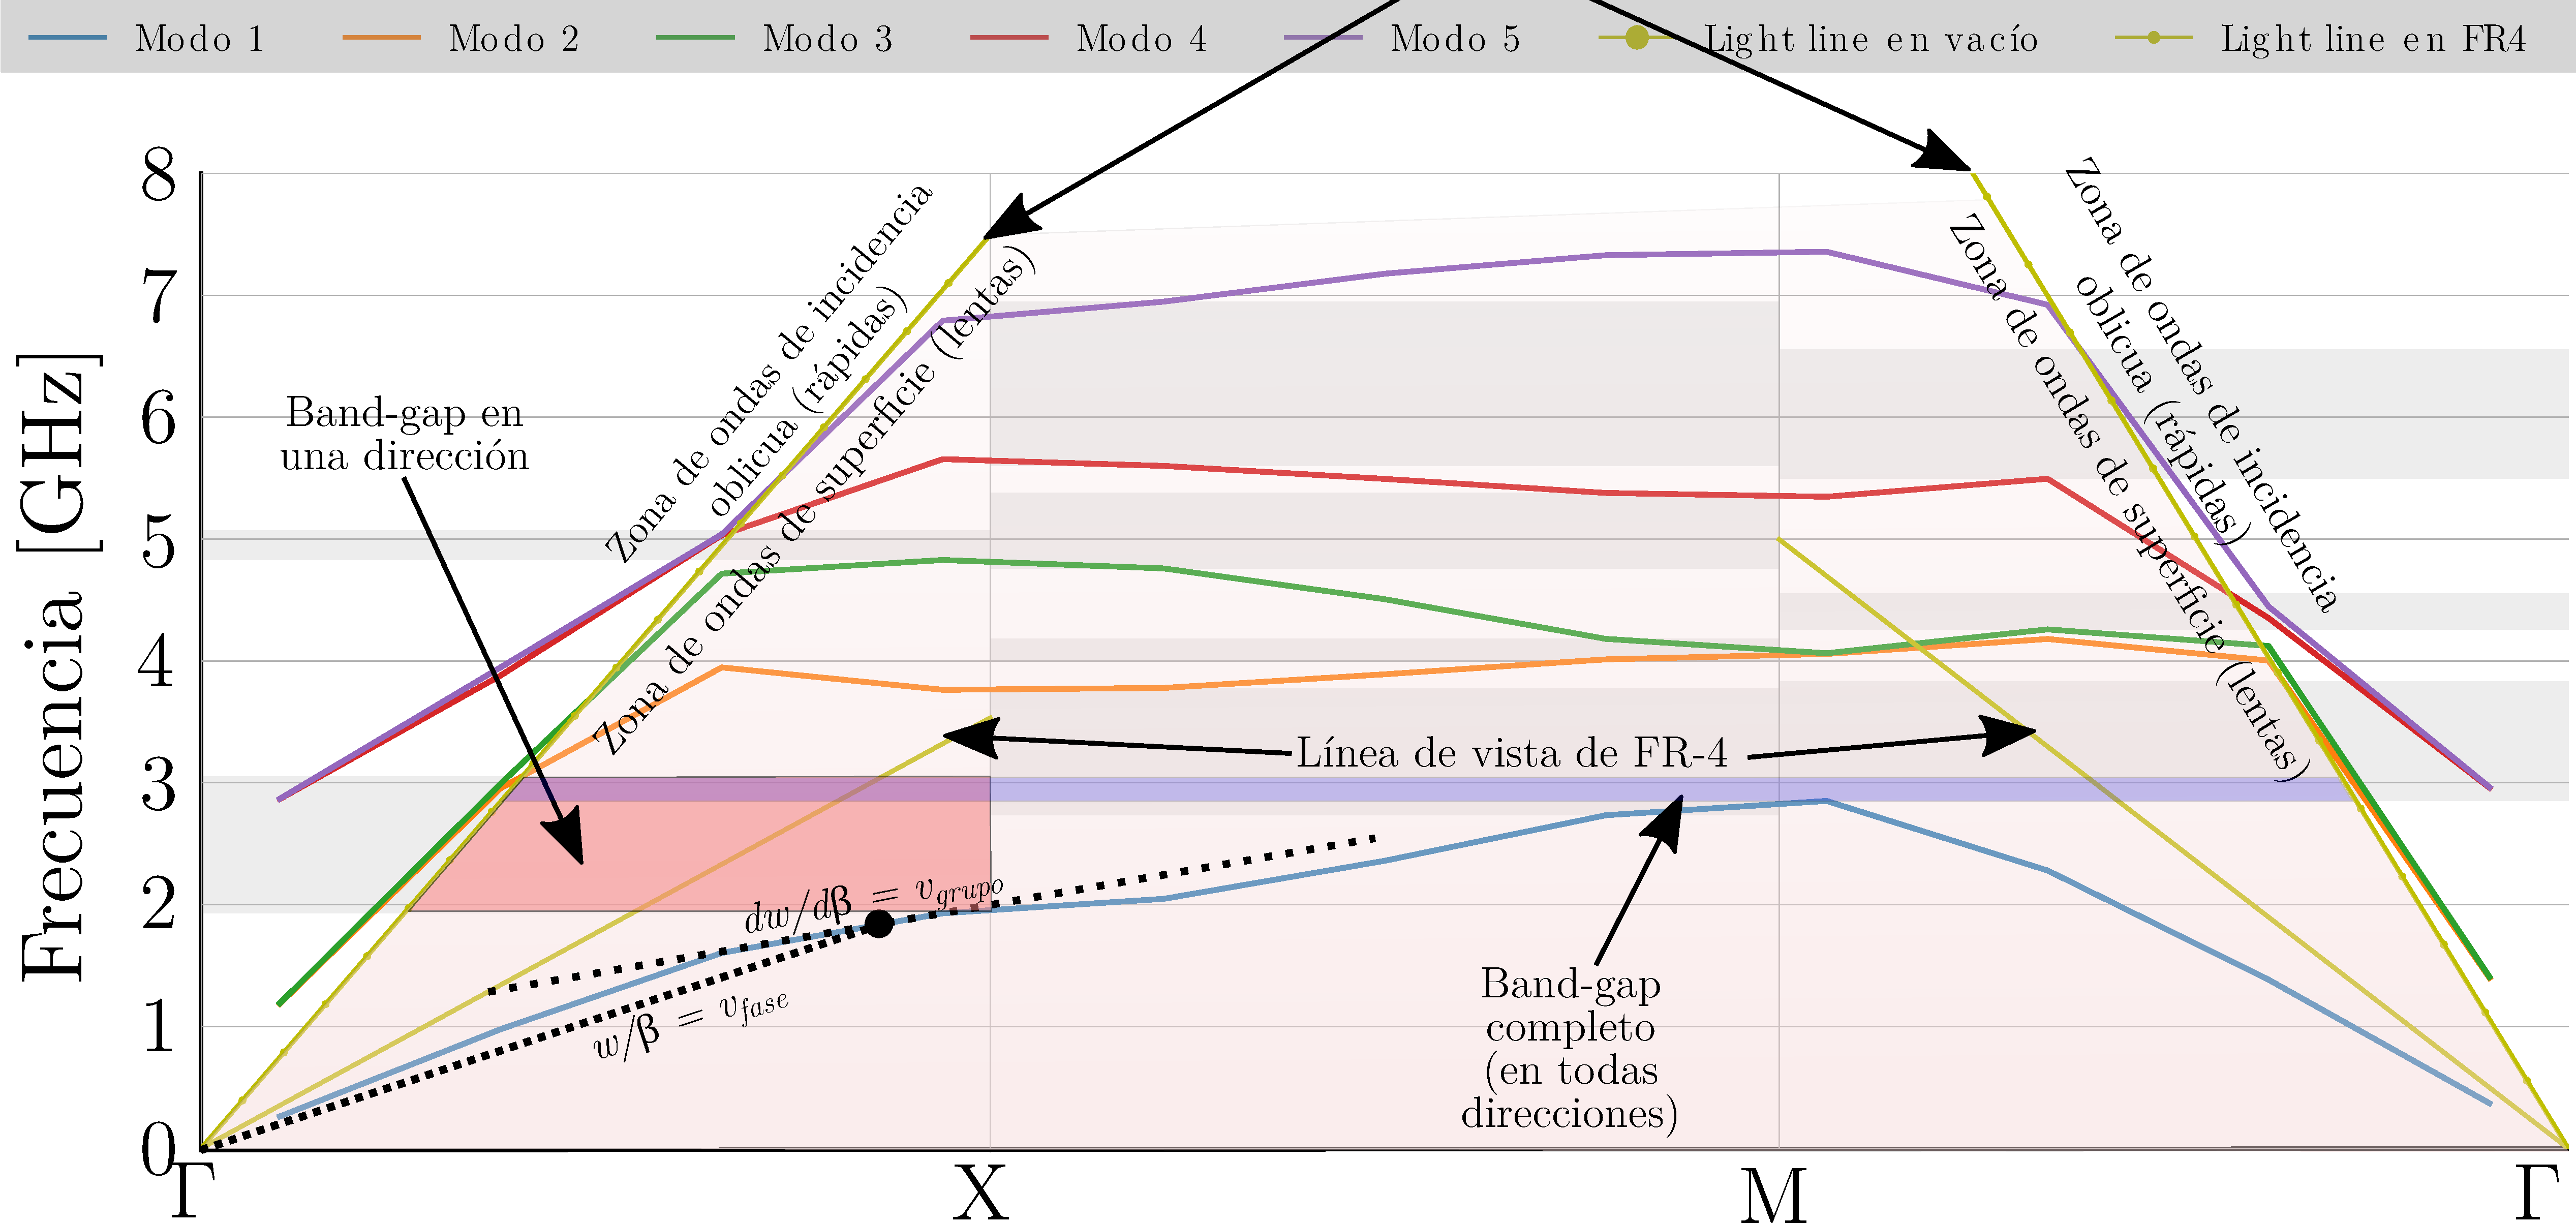
\includegraphics[width=\textwidth]{Modelado/ejemplo-diag-disp.pdf}
	\caption{Ejemplo típico de un diagrama de dispersión que presenta un metamaterial bidimensional.}
	\label{fig:diag-dispersion-tipico}
\end{figure}

La línea azul corresponde al primer modo de propagación, la marrón al segundo, la verde al tercero, la roja al cuarto y la violeta al quinto. Además, se dibujaron las líneas de vista (\textit{light-lines}) para vacío y para FR-4, que indican el comportamiento de una onda plana que circula por esos materiales. Representan el corte del diagrama de dispersión tridimensional mostrado en la figura \ref{fig:diagrama-dispersion-vacio-3d} sobre los bordes de la celda de Brillouin, como se ve en la figura \ref{fig:diagrama-dispersion-vacio-2d}, para los dos materiales. La línea de vista del FR-4 presenta, naturalmente, una pendiente menor a la del vacío, pues la velocidad de propagación sobre ese medio es menor.

La línea de vista del vacío separa las llamadas ondas lentas (\textit{slow waves}), que poseen una velocidad de fase menor a la del vacío ($c$), de las ondas rápidas (\textit{fast waves}), con velocidad de fase superior a $c$. Dado que, para el vacío, $\beta=\omega/c$, si se extiende a definición a dos dimensiones, se obtiene que $\beta_x^2 + \beta_y^2 = \omega^2/c^2$. Cuando el valor de $|\beta|$ supera al correspondiente a la propagación en el vacío para la misma frecuencia, necesariamente la velocidad de fase es menor ($\beta = \omega / v_p$). Cuando la velocidad es mayor, es decir, cuando se analizan resultados para pares $(\omega,\beta)$ que están por encima de la línea de vista, el estudio no se da sobre ondas de superficie, sino sobre ondas incidentes o reflejadas con ángulo determinado. En algunos casos \cite{Maci:Pole-zero-matching}, para algunos usos de metamateriales (especialmente cuando se los diseña de forma que actúen como paredes conductoras magnéticas), esa zona del diagrama de dispersión resulta de gran utilidad \cite{Yang:EBGAntennas}.

Las zonas demarcadas en gris representan, para cada una de las direcciones analizadas, la zona de frecuencias prohibidas o \textit{band-gap}. En particular, para la zona $\Gamma-X$, el primer \textit{band-gap} se demarcó en rojo. Se debe tener en cuenta que se calculan los \textit{band-gaps} para  las tres direcciones de forma separada. Existe un \textit{band-gap} completo (en azul), cuando existe en todas las direcciones analizadas. Para las frecuencias dentro de la zona prohibida completa, no existirá ángulo de incidencia que permita su propagación. Es importante notar que, para los intervalos $\Gamma-X$ y $M-\Gamma$, las zonas prohibidas para la propagación de ondas lentas (\textit{slow-waves}) de superficie se calculan por debajo de la línea de vista del vacío. Por encima de dicha línea, las ondas se propagan libremente.

En general, el diseño de EBGs tiene como objetivo aumentar el ancho de la banda prohibida de frecuencias para la propagación de ondas de superficie, la variación de la frecuencia central de los \textit{band-gaps}, y la independización del mismo de la dirección de propagación (que equivale a lograr \textit{band-gaps} completos). Estos objetivos se logran modificando la geometría de la celda unitaria, aumentando el acoplamiento entre las mismas y conectando los parches al plano de tierra \cite{Marcela:Tesis}. La independización de las zonas prohibidas para cualquier dirección azimutal de propagación de ondas de superficie requiere celdas simétricas, aunque para ciertas aplicaciones la anisotropía es buscada \cite{Maci:Pole-zero-matching}.

El diagrama de dispersión, además, da una idea de las velocidades de fase ($v_p = w/\beta$) y grupo ($v_g = d\omega / d\beta$) para los modos existentes.

%% Analizar Vfase, Vg, y por qué cambian según la posición en el diagrama de briloouin. Ver Mohajer-Irarani, Ramahi. Esto va de la mano con ¿por qué los ebgs son tanto más chico que lambda? porque la velocidad de propagación es menor adentr del sustrato, en los modos atrapadao. Eso se puede ver en Goussetis, Feresidis, Vardaxoglow (periodically loaded 1 D metallodielectric..). Vincular con el tema de Forward y Backward waves (Kubacki, Lamari, Rudyk).

%% Se debe tener en cuenta que un bandgap no indica que no hay transferencia de poencia. Puede hacer un bandgap, que significa que no hay ondas propagantes, pero sí existen ondas evanescentes, que pueden, si llegan con suficiente energía, excitar a celdas cercanas y generar leaky waves y transporte de potencia. Es un gran problema. Ver Mohajer-Irarani, Ramahi.

%%%% ESTARRIA MUY BUENO EN ALGUN MOMENTO PONER UN DIAGRAMA DE DISPERSION DE UN SLAB DESNUDO Y OTRO DE UN SLAB CON DIELECTRICO; PARA UNIIR CON LA PARTE TEÓRICA ANTERIOR.

\subsubsection{Efecto de la variación del ancho del puente \textit{microstrip}}

La primera variación analizada es la del ancho de los puentes \textit{microstrip} que unen a los parches metálicos que conforman la estructura. Estableciendo una celda de $2\;\text{cm}$ de lado, y un parche de $1.8\;\text{cm}$, para el caso de sustrato FR4 de $1.6\;\text{mm}$ de espesor, se obtuvieron los diagramas de dispersión sobre el borde de la celda de Brillouin que se muestran en la figura \ref{fig:diagdisp-orlandi-variacion-ancho-puente}.

\begin{figure}[h]
	\centering
	\includegraphics[width=1\textwidth]{Modelado/Orlandi-DeltaAnchoConector.pdf}
	\caption{Diagramas de dispersión para la variación del ancho de los puentes \textit{microstrip} que conforman una celda unitaria cuadrada, de lado $2\;\text{cm}$, parche de $1.8\;\text{cm}$, con sustrato de FR-4 de $1.6\;\text{mm}$ de espesor.}
	\label{fig:diagdisp-orlandi-variacion-ancho-puente}
\end{figure}

En la misma se observa que la formación de una zona prohibida completa entre los dos primeros modos de propagación, se ve dificultada cuando el ancho del puente aumenta, debido a que, para todas las direcciones de propagación, el ancho de los \textit{band-gaps} disminuye drásticamente.


\begin{figure}[h]
	\centering
	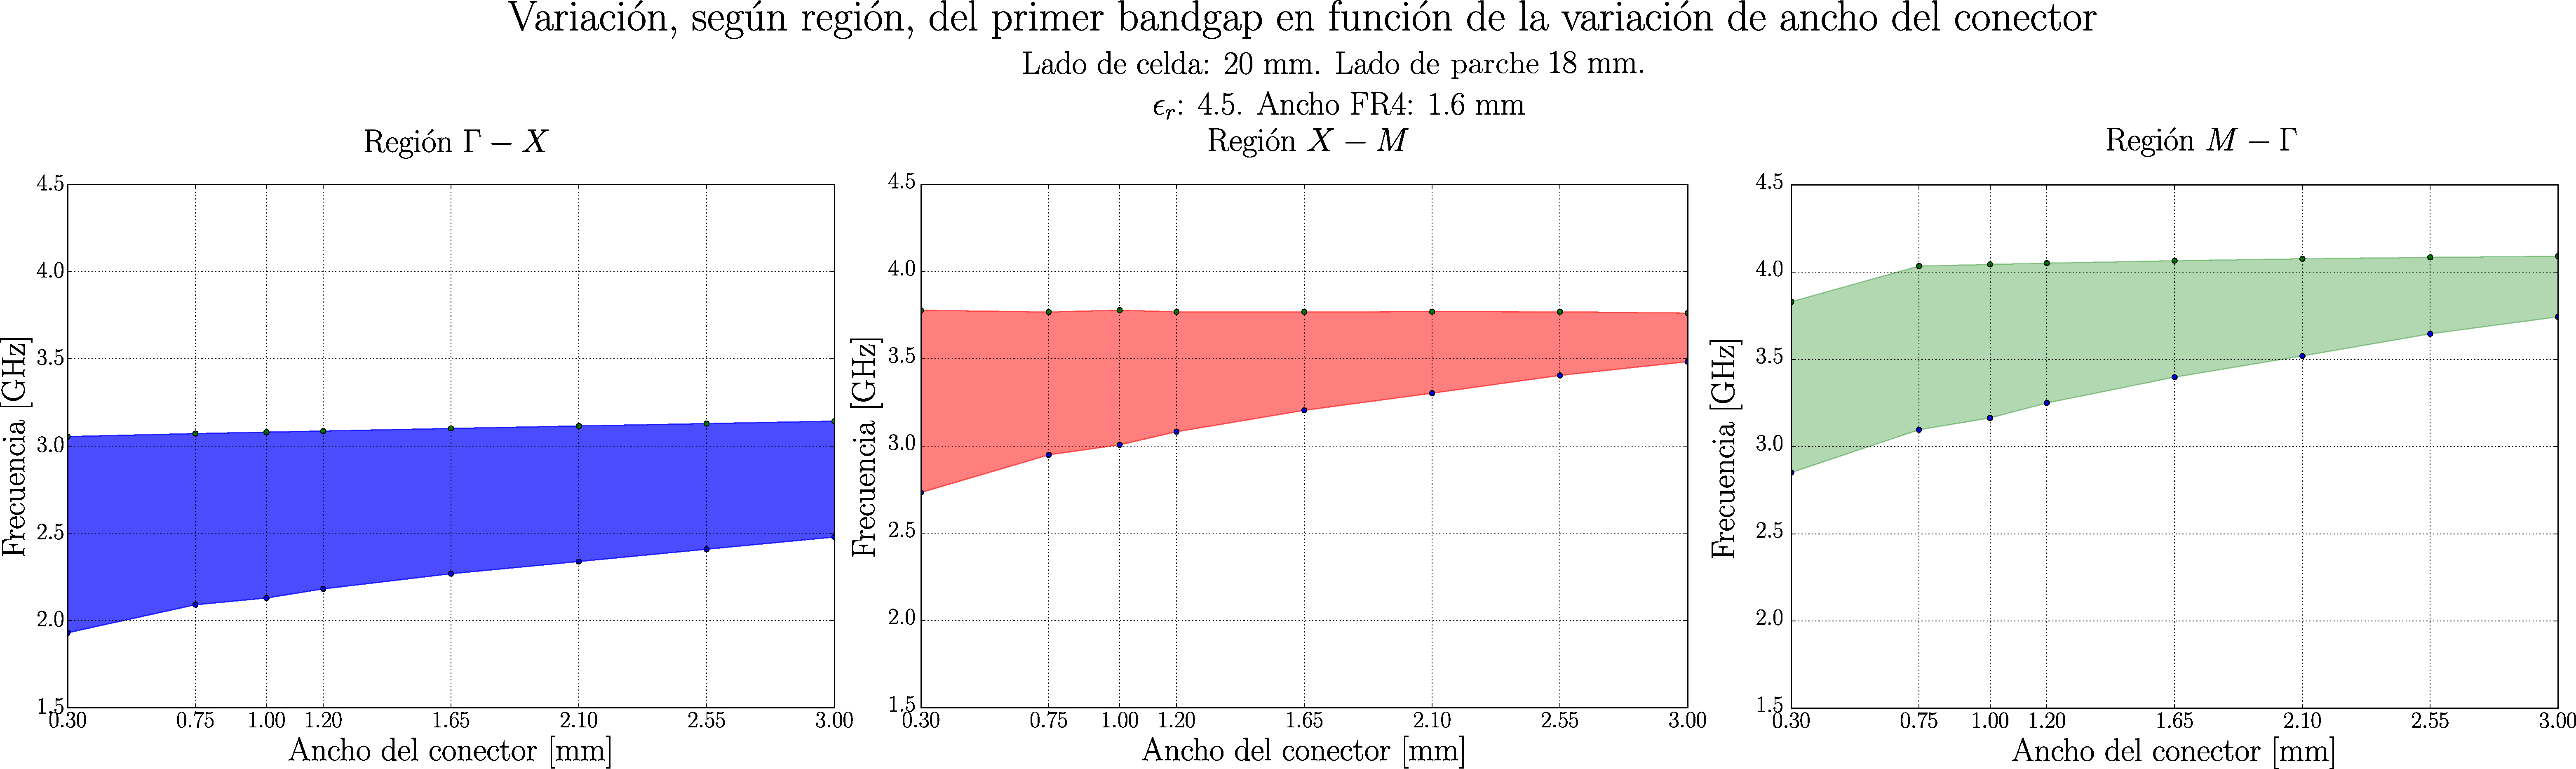
\includegraphics[width=1\textwidth]{Modelado/Orlandi-DeltaAnchoConector-comparacion.pdf}
	\caption{Comparación del ancho del primer band-gap (entre el primer y el segundo modo de propagación) para las tres direcciones analizadas, en función del ancho del puente que une los parches metálicos.}
	\label{fig:comparacion-diagdisp-orlandi-variacion-ancho-puente}
\end{figure}

La principal causa se puede deducir de la figura \ref{fig:comparacion-diagdisp-orlandi-variacion-ancho-puente}, donde es notorio el crecimiento generalizado de las frecuencias necesarias para obtener el primer modo de propagación (la curva azul de la figura \ref{fig:diagdisp-orlandi-variacion-ancho-puente} se eleva), lo que se condice con una aumento en la velocidad de propagación en el metamaterial. Una explicación intuitiva, válida únicamente para las frecuencias en que se puede aplicar el modelo cuasiestático y considerar corrientes y tensiones sobre los conductores que conforman la estructura, se basa en la posible disminución de la resistencia al paso de corriente, lo que permite una carga y descarga del capacitor de placas planas paralelas (formado por el parche y el plano de tierra) más rápida.

Para modos superiores, especialmente para el rango de frecuencias entre el cuarto y el quinto modo, existe una zona prohibida que se extiende en todas direcciones, pero se da para frecuencias mucho más altas, de escaso valor práctico.

\clearpage
\subsubsection{Efecto del escalamiento de la celda unitaria}

\begin{figure}[h]
	\centering
	\includegraphics[width=1\textwidth]{Modelado/Orlandi-DeltaTamanioCelda-RelacionParcheFija.pdf}
	\caption{Diagramas de dispersión para la variación del ancho de las celdas unitarias (y, en consecuencia, también del parche que contiene) que conforman una celda unitaria cuadrada. El lado del parche es $3/4$ del lado de la celda unitaria. El sustrato de FR-4 de $1.6\;\text{mm}$ de espesor.}
	\label{fig:diagdisp-orlandi-variacion-tam-celda-unitaria}
\end{figure}

\begin{figure}[h]
	\centering
	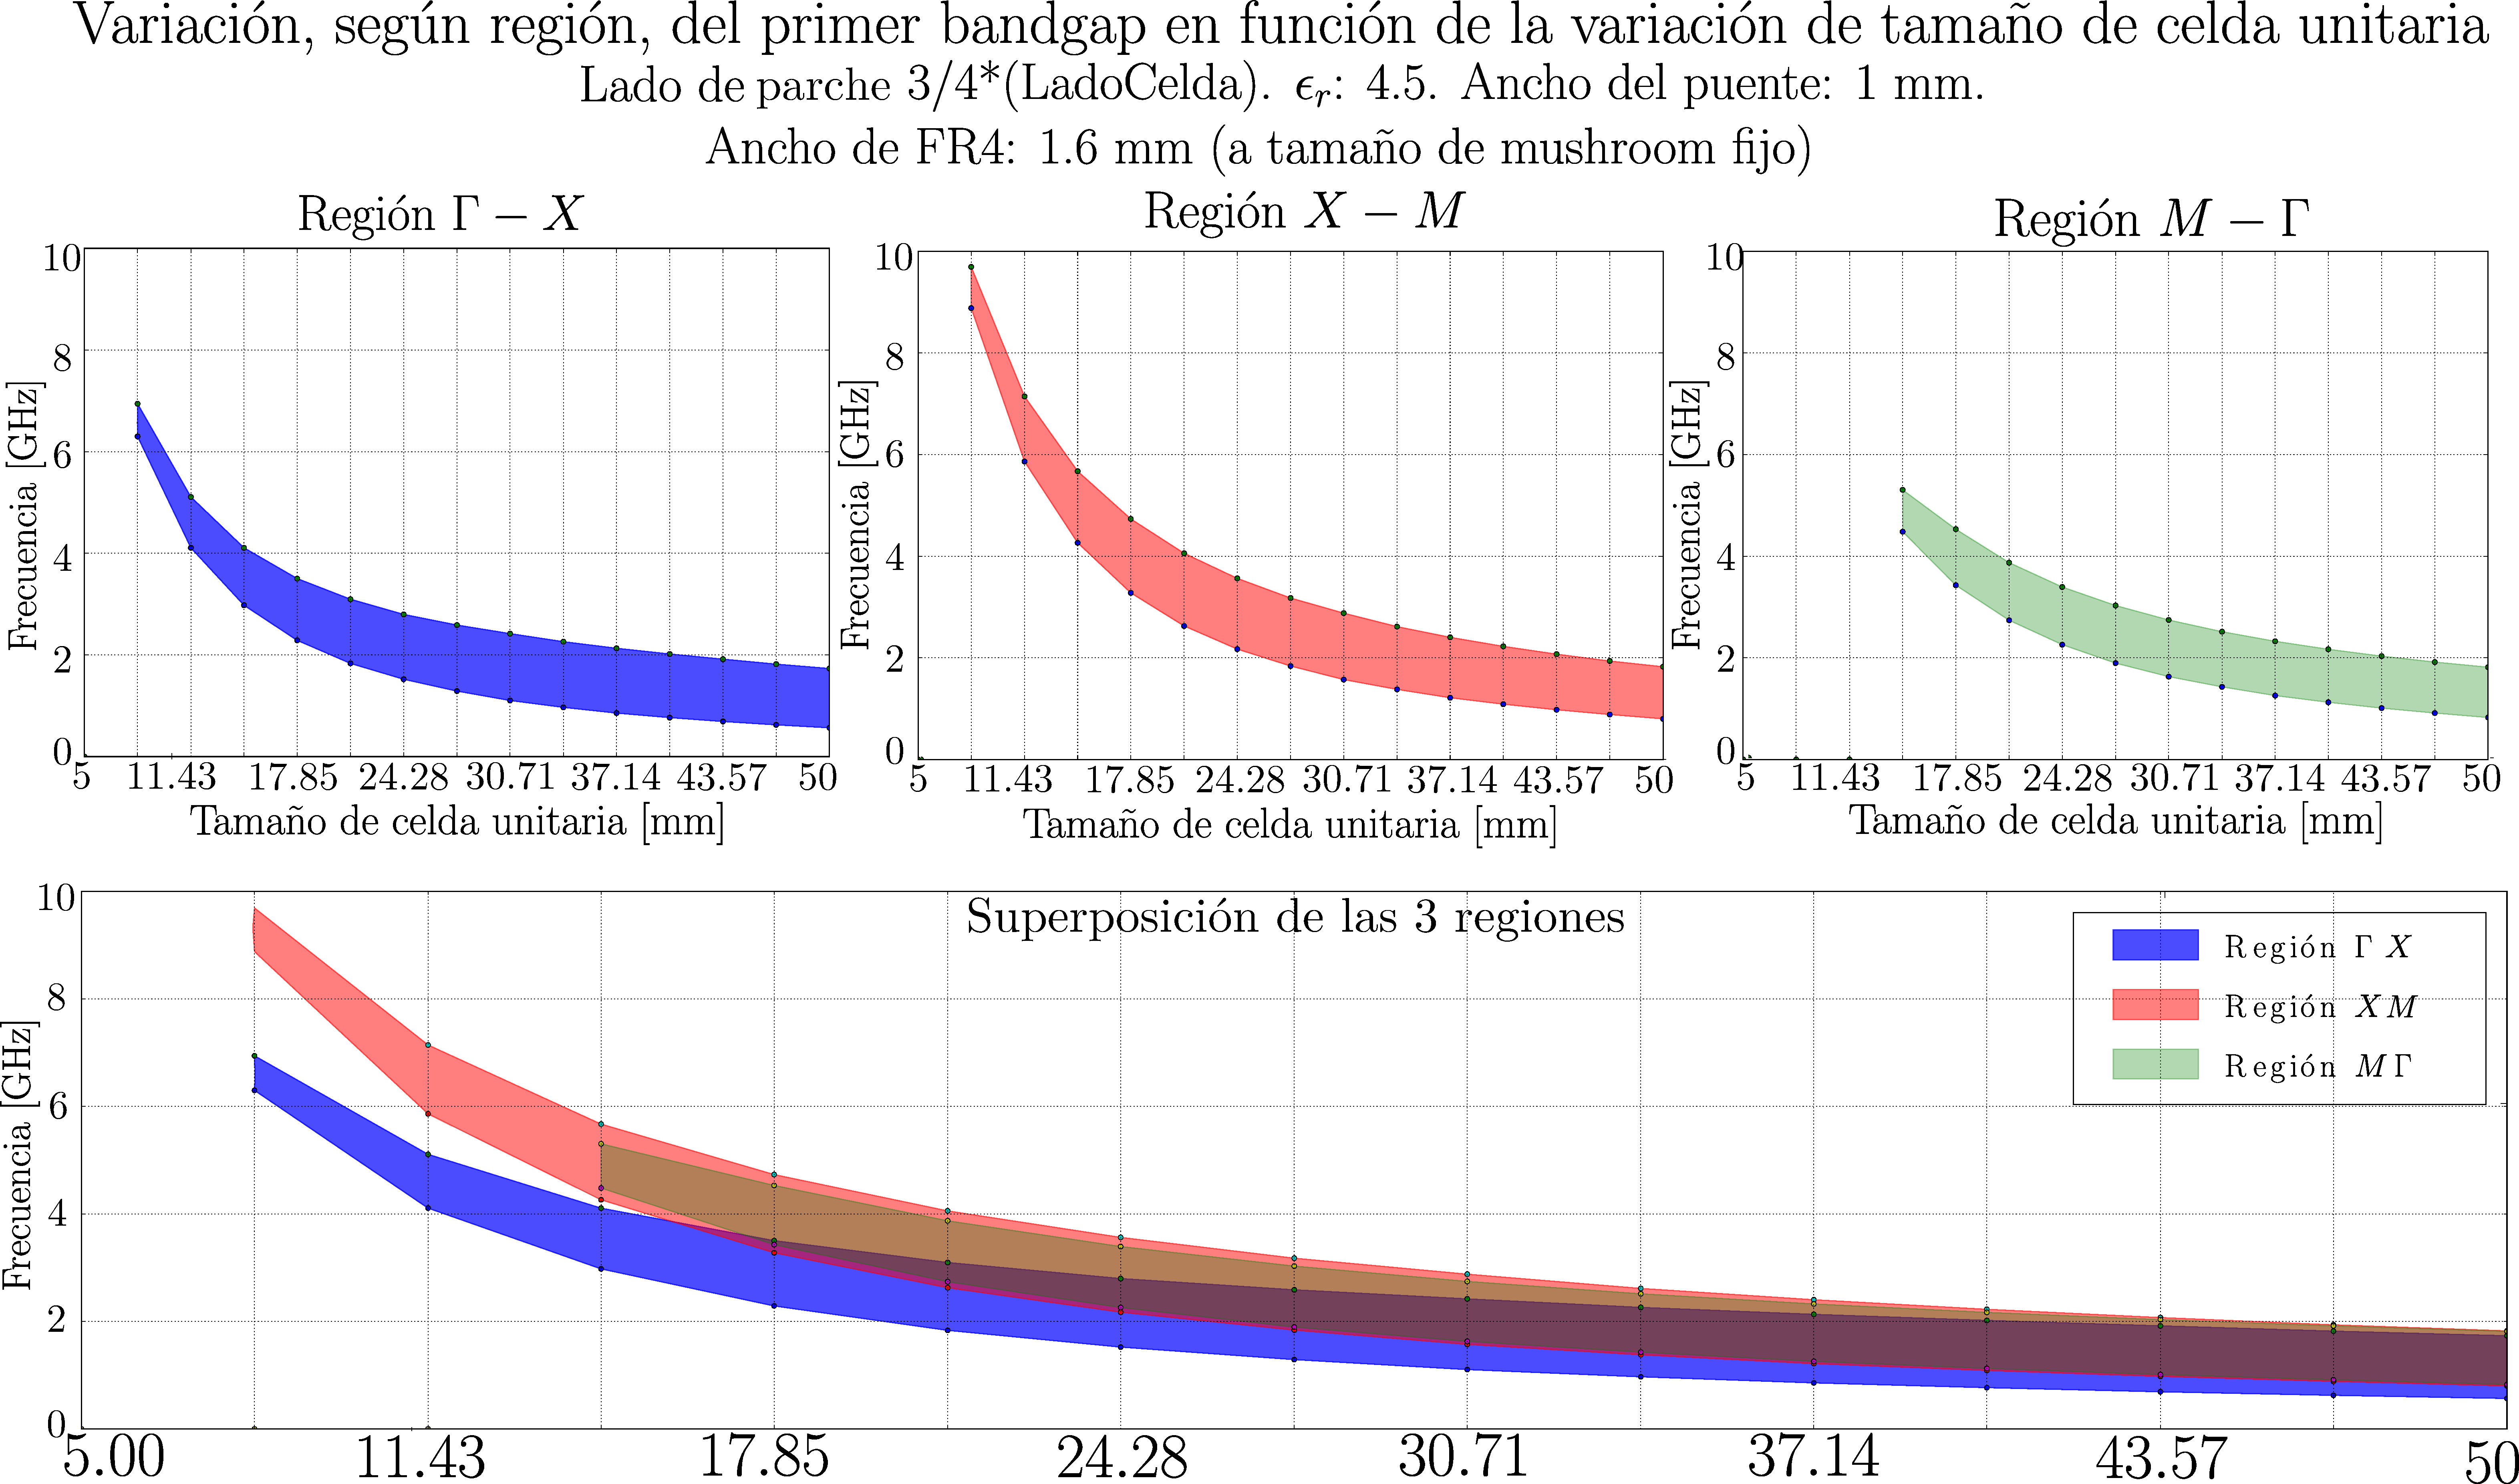
\includegraphics[width=1\textwidth]{Modelado/Orlandi-DeltaTamanioCelda-RelacionParcheFija-Comparacion.pdf}
	\caption{Compraración del ancho del primer band-gap (entre el primer y el segundo modo de propagación) para las tres direcciones analizadas, en función del tamaño de la celda unitaria.}
	\label{fig:comparacion-diagdisp-orlandi-variacion-tam-celda-unitaria}
\end{figure}

Un escalamiento de la celda unitaria, debido a la linealidad de las ecuaciones de Maxwell, debería únicamente generar un cambio en las frecuencias centrales de los \textit{band-gaps}. Para celdas unitarias pequeñas, las frecuencias centrales de las zonas prohibidas son altas, y resulta más difícil obtener un \textit{bandgap} completo, como se observa en la figura \ref{fig:diagdisp-orlandi-variacion-tam-celda-unitaria}.

En la figura \ref{fig:comparacion-diagdisp-orlandi-variacion-tam-celda-unitaria} se puede observar el comportamiento del primer \textit{bandgap} (ubicado entre el primer y el segundo modo de propagación), en función del tamaño de la celda unitaria analizada. A medida que la misma disminuye, las frecuencias centrales decaen a un ritmo de $sarasa$. La variación del tamaño de la celda unitaria, por sí solo, facilita la superposición de zonas prohibidas en todas las direcciones sólo para frecuencias bajas, y cuando la celda unitaria es grande. La superposición de las tres direcciones de propagación analizadas se puede observar en la gráfica inferior de la figura \ref{fig:comparacion-diagdisp-orlandi-variacion-tam-celda-unitaria}.

El comportamiento de la primer zona prohibida se puede explicar intuitivamente considerando que, de no variar la velocidad de propagación en el medio, y dado que $\omega =k*v_p$, entonces al variar el número de onda requerido por aumentar el tamaño de la celda unitaria (disminuye, permitiendo que el primer modo se corresponda con una longitud de onda mayor), el valor de $\omega$ debe disminuir en consecuencia.

A este efecto se debe añadir el correspondiente al aumento del efecto capacitivo por el aumento del tamaño del parche. Si se considera, como se explicó antes, que un análisis a bajas frecuencias, utilizando razonamientos cuasiestáticos, nos conduce a un filtro LC equivalente. La frecuencia de resonancia de ese tipo de filtro es, en general, y sin considerar pérdidas, $f_r \approx 1/\sqrt{LC}$. Dado que se está escalonando la celda unitaria, y que por tanto también está creciendo el tamaño del parche, el valor de la capacidad aumenta. La relación entre la capacidad y el tamaño del parche es cuadrática, como se puede ver en la ecuación \ref{eq:Cp_Lp}, y la inductancia no aumentará apreciablemente en comparación. De esta forma: $f_r \propto 1/\sqrt{l^2} = 1/l$, con $l$ el tamaño del parche, según la figura \ref{fig:celda-orlandi}.

Resulta importante destacar que la variación del tamaño de la celda unitaria en su conjunto es la forma más fácil (aunque en general, la menos conveniente) de modificar la frecuencia de trabajo del EBG.

\clearpage

\subsubsection{Efecto de la variación del tamaño del parche metálico}

\begin{figure}[h]
	\centering
	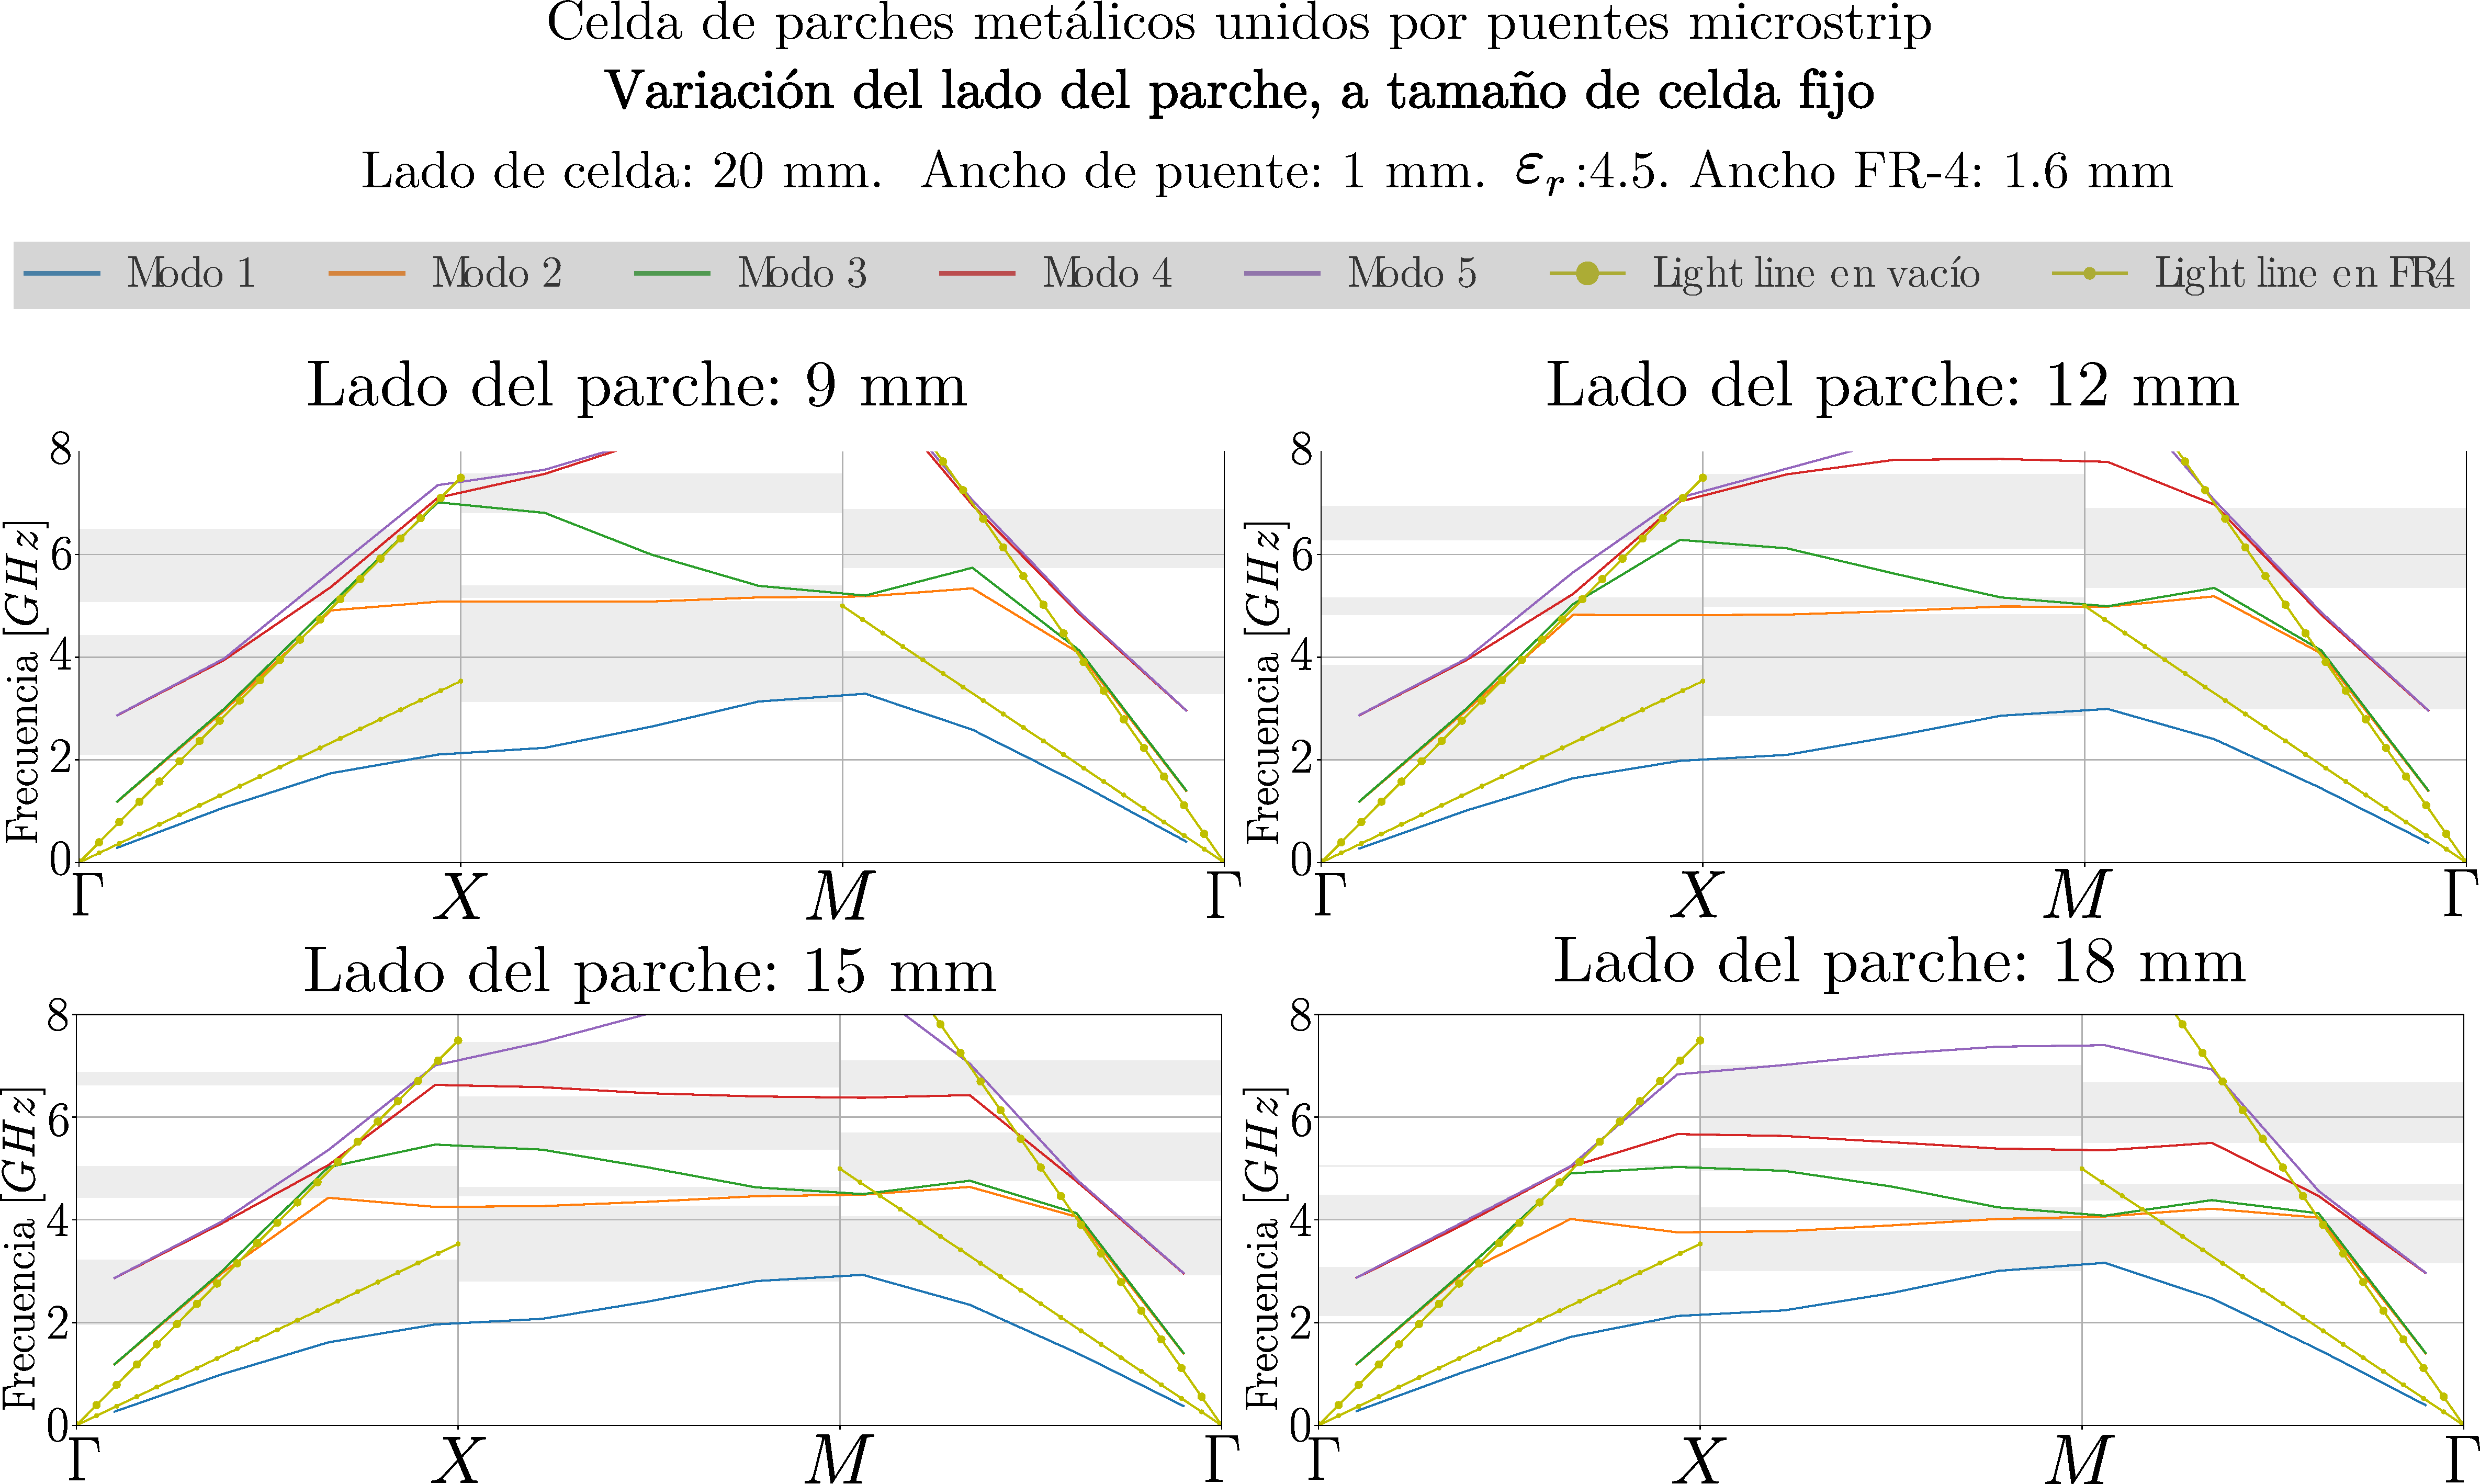
\includegraphics[width=1\textwidth]{Modelado/Orlandi-DeltaParcheMetalicoCeldaFija.pdf}
	\caption{Diagramas de dispersión para la variación del tamaño del parche metálico, sin una variación en el tamaño de la celda unitaria. El sustrato de FR-4 de $1.6\;\text{mm}$ de espesor.}
	\label{fig:diagdisp-orlandi-variacion-tam-parche}
\end{figure}


\begin{figure}[h]
	\centering
	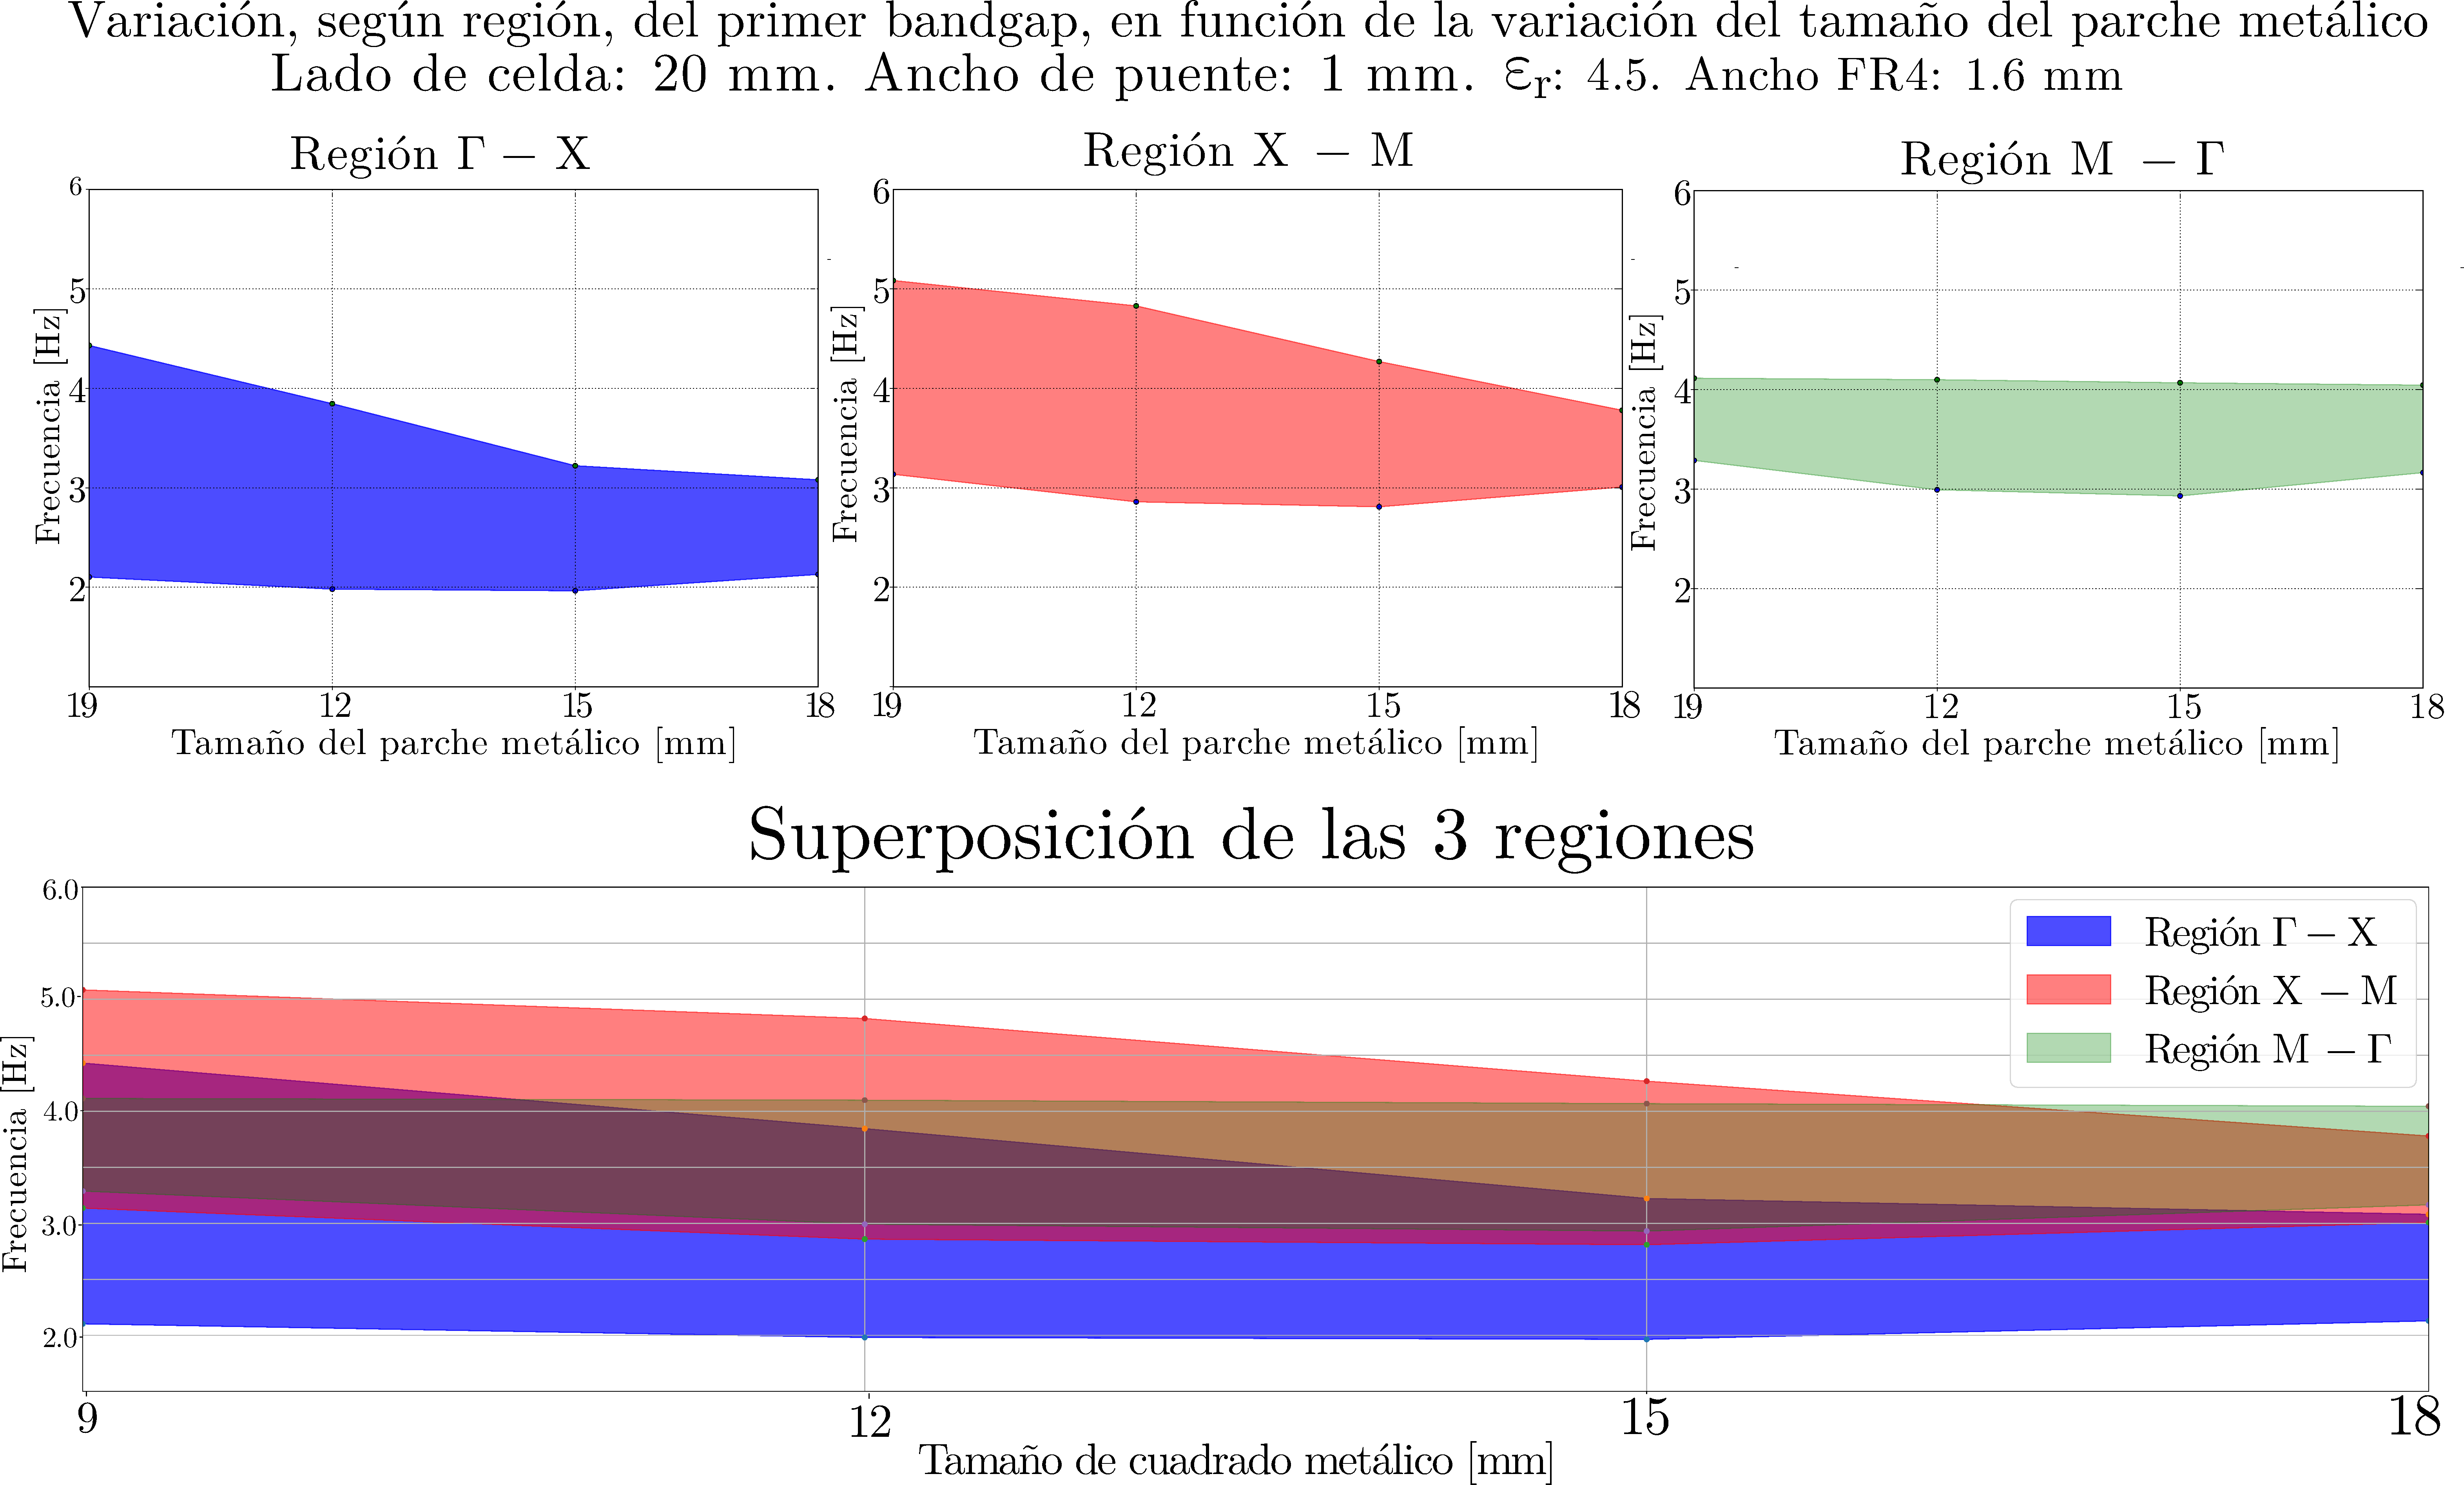
\includegraphics[width=1\textwidth]{Modelado/Orlandi-DeltaParcheMetalicoCeldaFija-Comparacion.pdf}
	\caption{Compraración del ancho del primer band-gap (entre el primer y el segundo modo de propagación) para las tres direcciones analizadas, en función del tamaño del parche.}
	\label{fig:comparacion-diagdisp-orlandi-variacion-tam-parche}
\end{figure}

La figura \ref{fig:diagdisp-orlandi-variacion-tam-parche} muestra que, al contrario que en el caso anterior, la mera variación del tamaño del parche metálico, sin la modificación del tamaño de la celda unitaria, no genera los mismos efectos. La variación de la capacidad, como antes, da lugar a una disminución en la frecuencia central del primer \textit{bandgap}.

Por otro lado, la inductancia impuesta por los puentes disminuye considerablemente cuando el tamaño del parche aumenta sin que lo haya la celda unitaria en general. En este sentido, manteniendo la analogía con el filtro LC presentado antes, dado que el ancho de banda de resonancia de un filtro LC es aproxidamente $BW_r \approx \sqrt{L/C}$, si disminuye el valor de la inductancia (por puentes más cortos) y, al mismo tiempo, aumenta el valor de la capacidad (por el aumento del efecto de capacitor de placas planas paralelas y las capacidades mutuas entre celdas vecinas) , el ancho de banda disminuirá notablemente.

Como se puede ver en la figura \ref{fig:comparacion-diagdisp-orlandi-variacion-tam-parche}, un mayor ancho de banda prohibida se obtiene con parches de tamaño moderado, con los que además es posible obtener bandas prohibidas completas.


\subsubsection{Variación de la longitud de los puentes}


\begin{figure}[h]
	\centering
	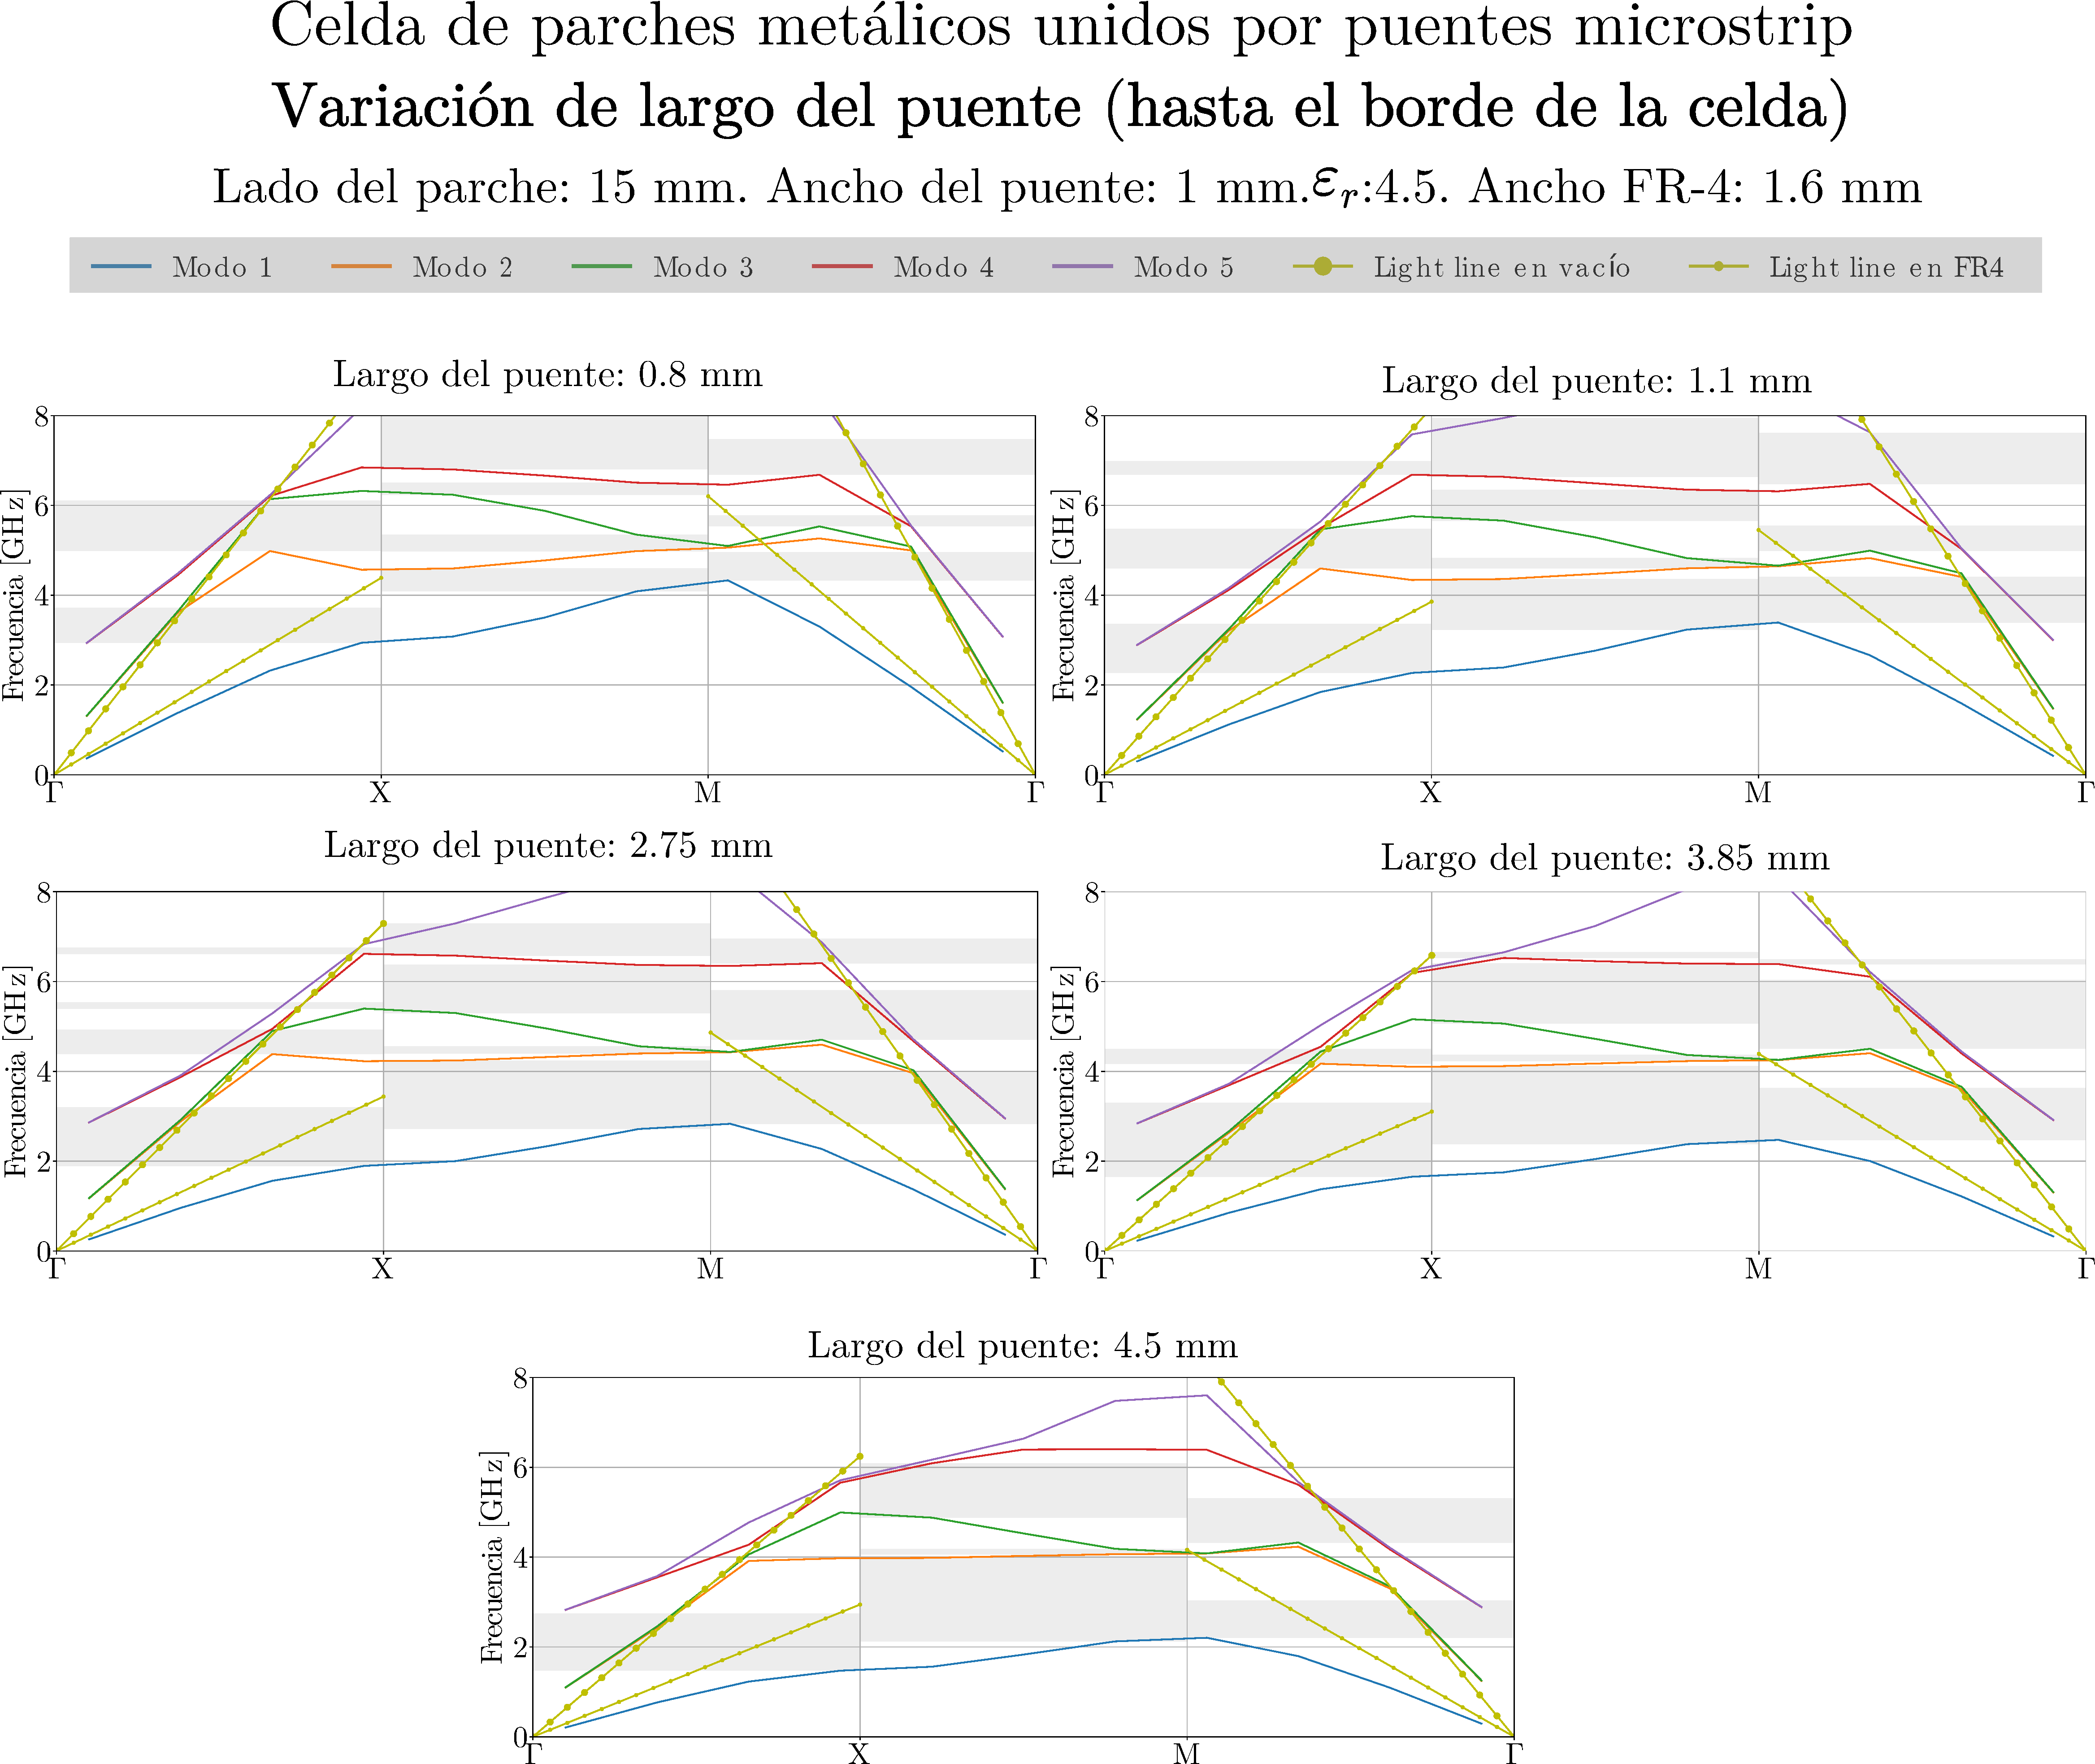
\includegraphics[width=1\textwidth]{Modelado/Orlandi-DeltaSeparacionParches-DeltaTamanioCelda-ParcheFijo.pdf}
	\caption{Diagramas de dispersión para la variación del largo de los puentes, que equivale a un aumento del tamaño de la celda unitaria, si las dimensiones del parche \textit{microstrip} se mantienen fijas. El sustrato de FR-4 de $1.6\;\text{mm}$ de espesor.}
	\label{fig:diagdisp-orlandi-variacion-long-puentes}
\end{figure}



\begin{figure}[h]
	\centering
	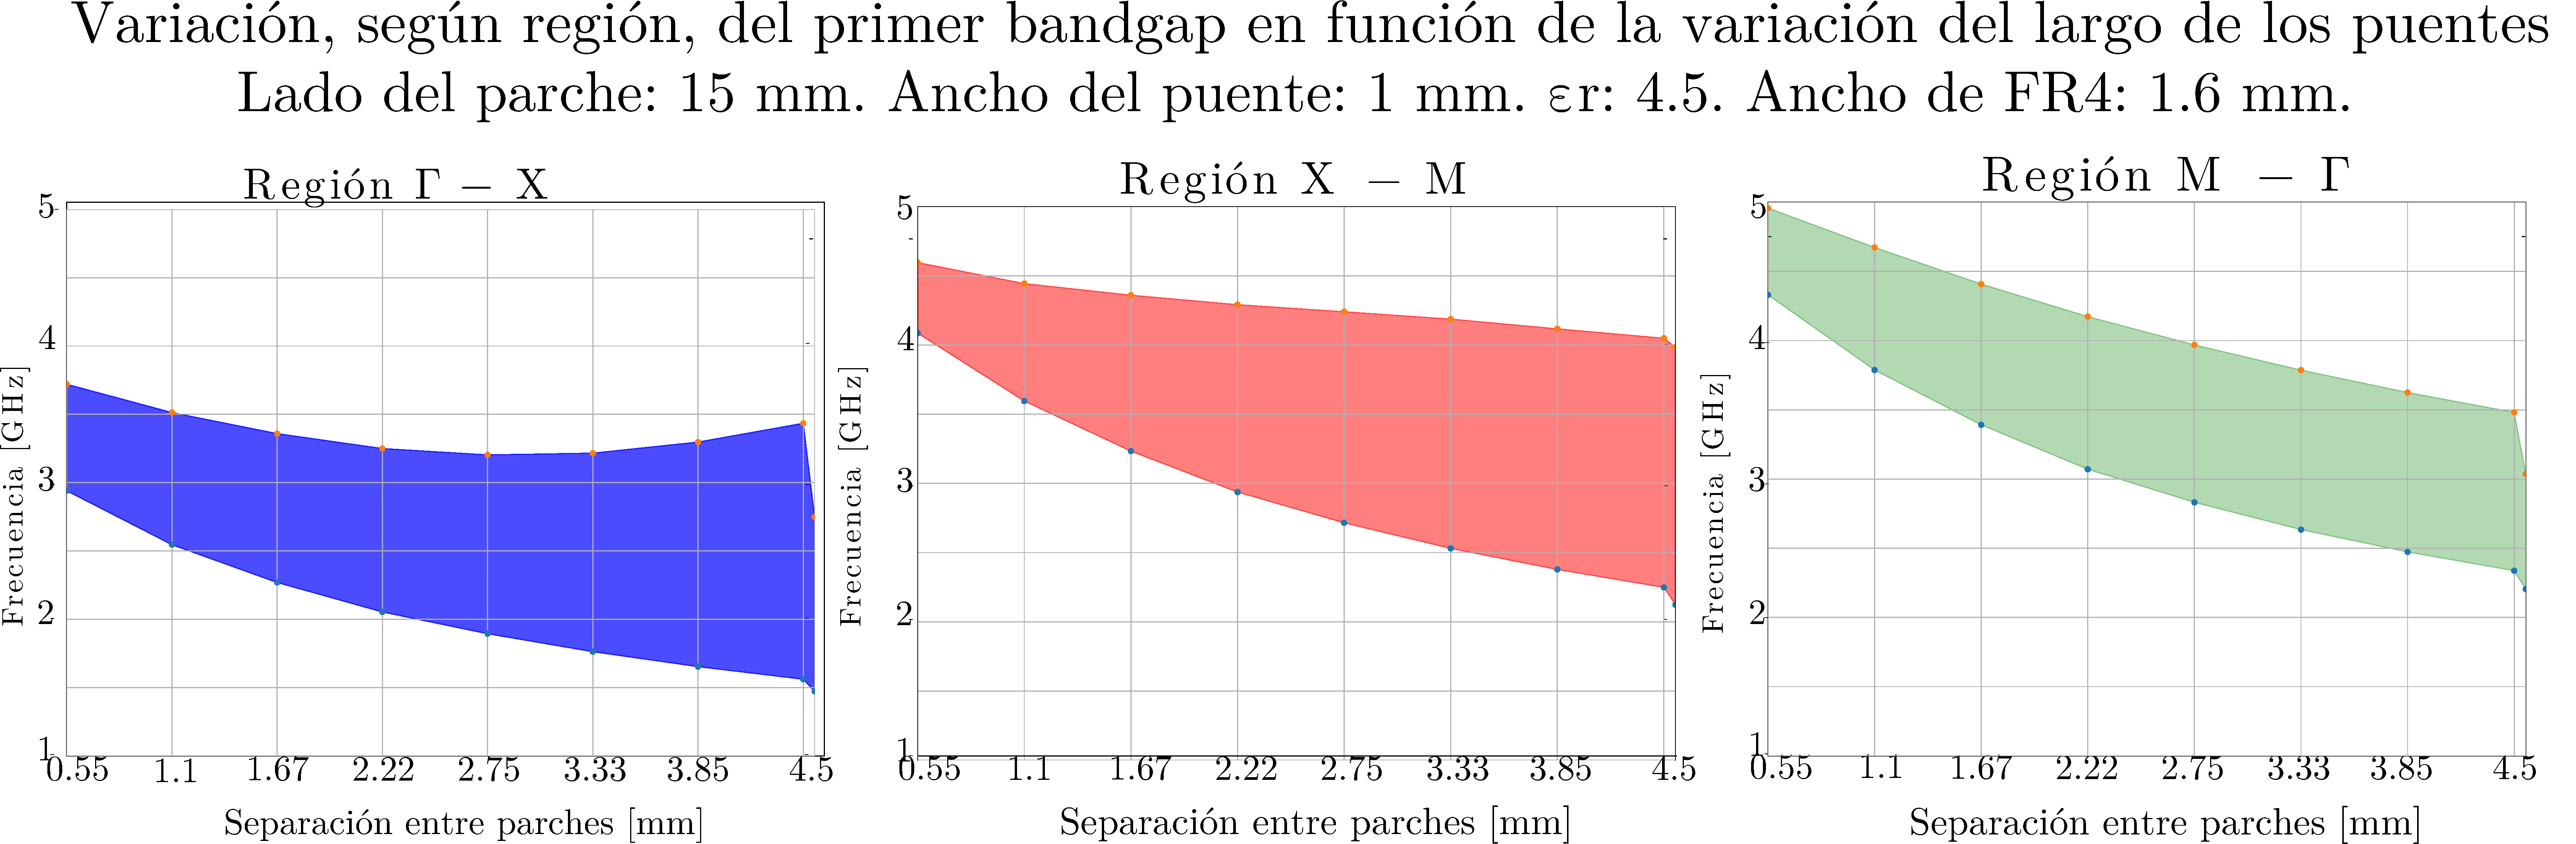
\includegraphics[width=1\textwidth]{Modelado/Orlandi-DeltaSeparacionParches-DeltaTamanioCelda-ParcheFijo-Comparacion.pdf}
	\caption{Compraración del ancho del primer band-gap (entre el primer y el segundo modo de propagación) para las tres direcciones analizadas, en función del largo de los puentes que unen a los parches.}
	\label{fig:comparacion-diagdisp-orlandi-long-puentes}
\end{figure}


Para la variación de la longitud de los puentes es necesario, nuevamente, modificar el tamaño de la celda unitaria, por lo que, necesariamente, a medida que exista una mayor separación entre los parches (y por tanto una mayor longitud de puentes), la frecuencia central de la banda prohibida disminuirá.

Por otro lado, dado que la capacidad no cambiará (excepto aquella correspondiente al efecto de capacidad entre parches cercanos, que estarán cada vez más alejados), los efectos más notorios, bajo un análisis cuasiestático, se darán por el aumento de la inductancia. El alejamiento de los parches metálicos entre sí disminuirá la capacidad total de cada celda unitaria, pero los efectos no son lo suficientemente notorios. Si los puentes no exisitieran, el efecto sería el opuesto al que se da en esta geometría \cite{Yang:EBGAntennas}. Este aumento en la inductancia generará un mayor ancho de banda, que se ve reflejado en la figura \ref{fig:comparacion-diagdisp-orlandi-long-puentes}.

\subsubsection{Efecto de la variación del ancho del sustrato dieléctrico}

\begin{figure}[h]
	\centering
	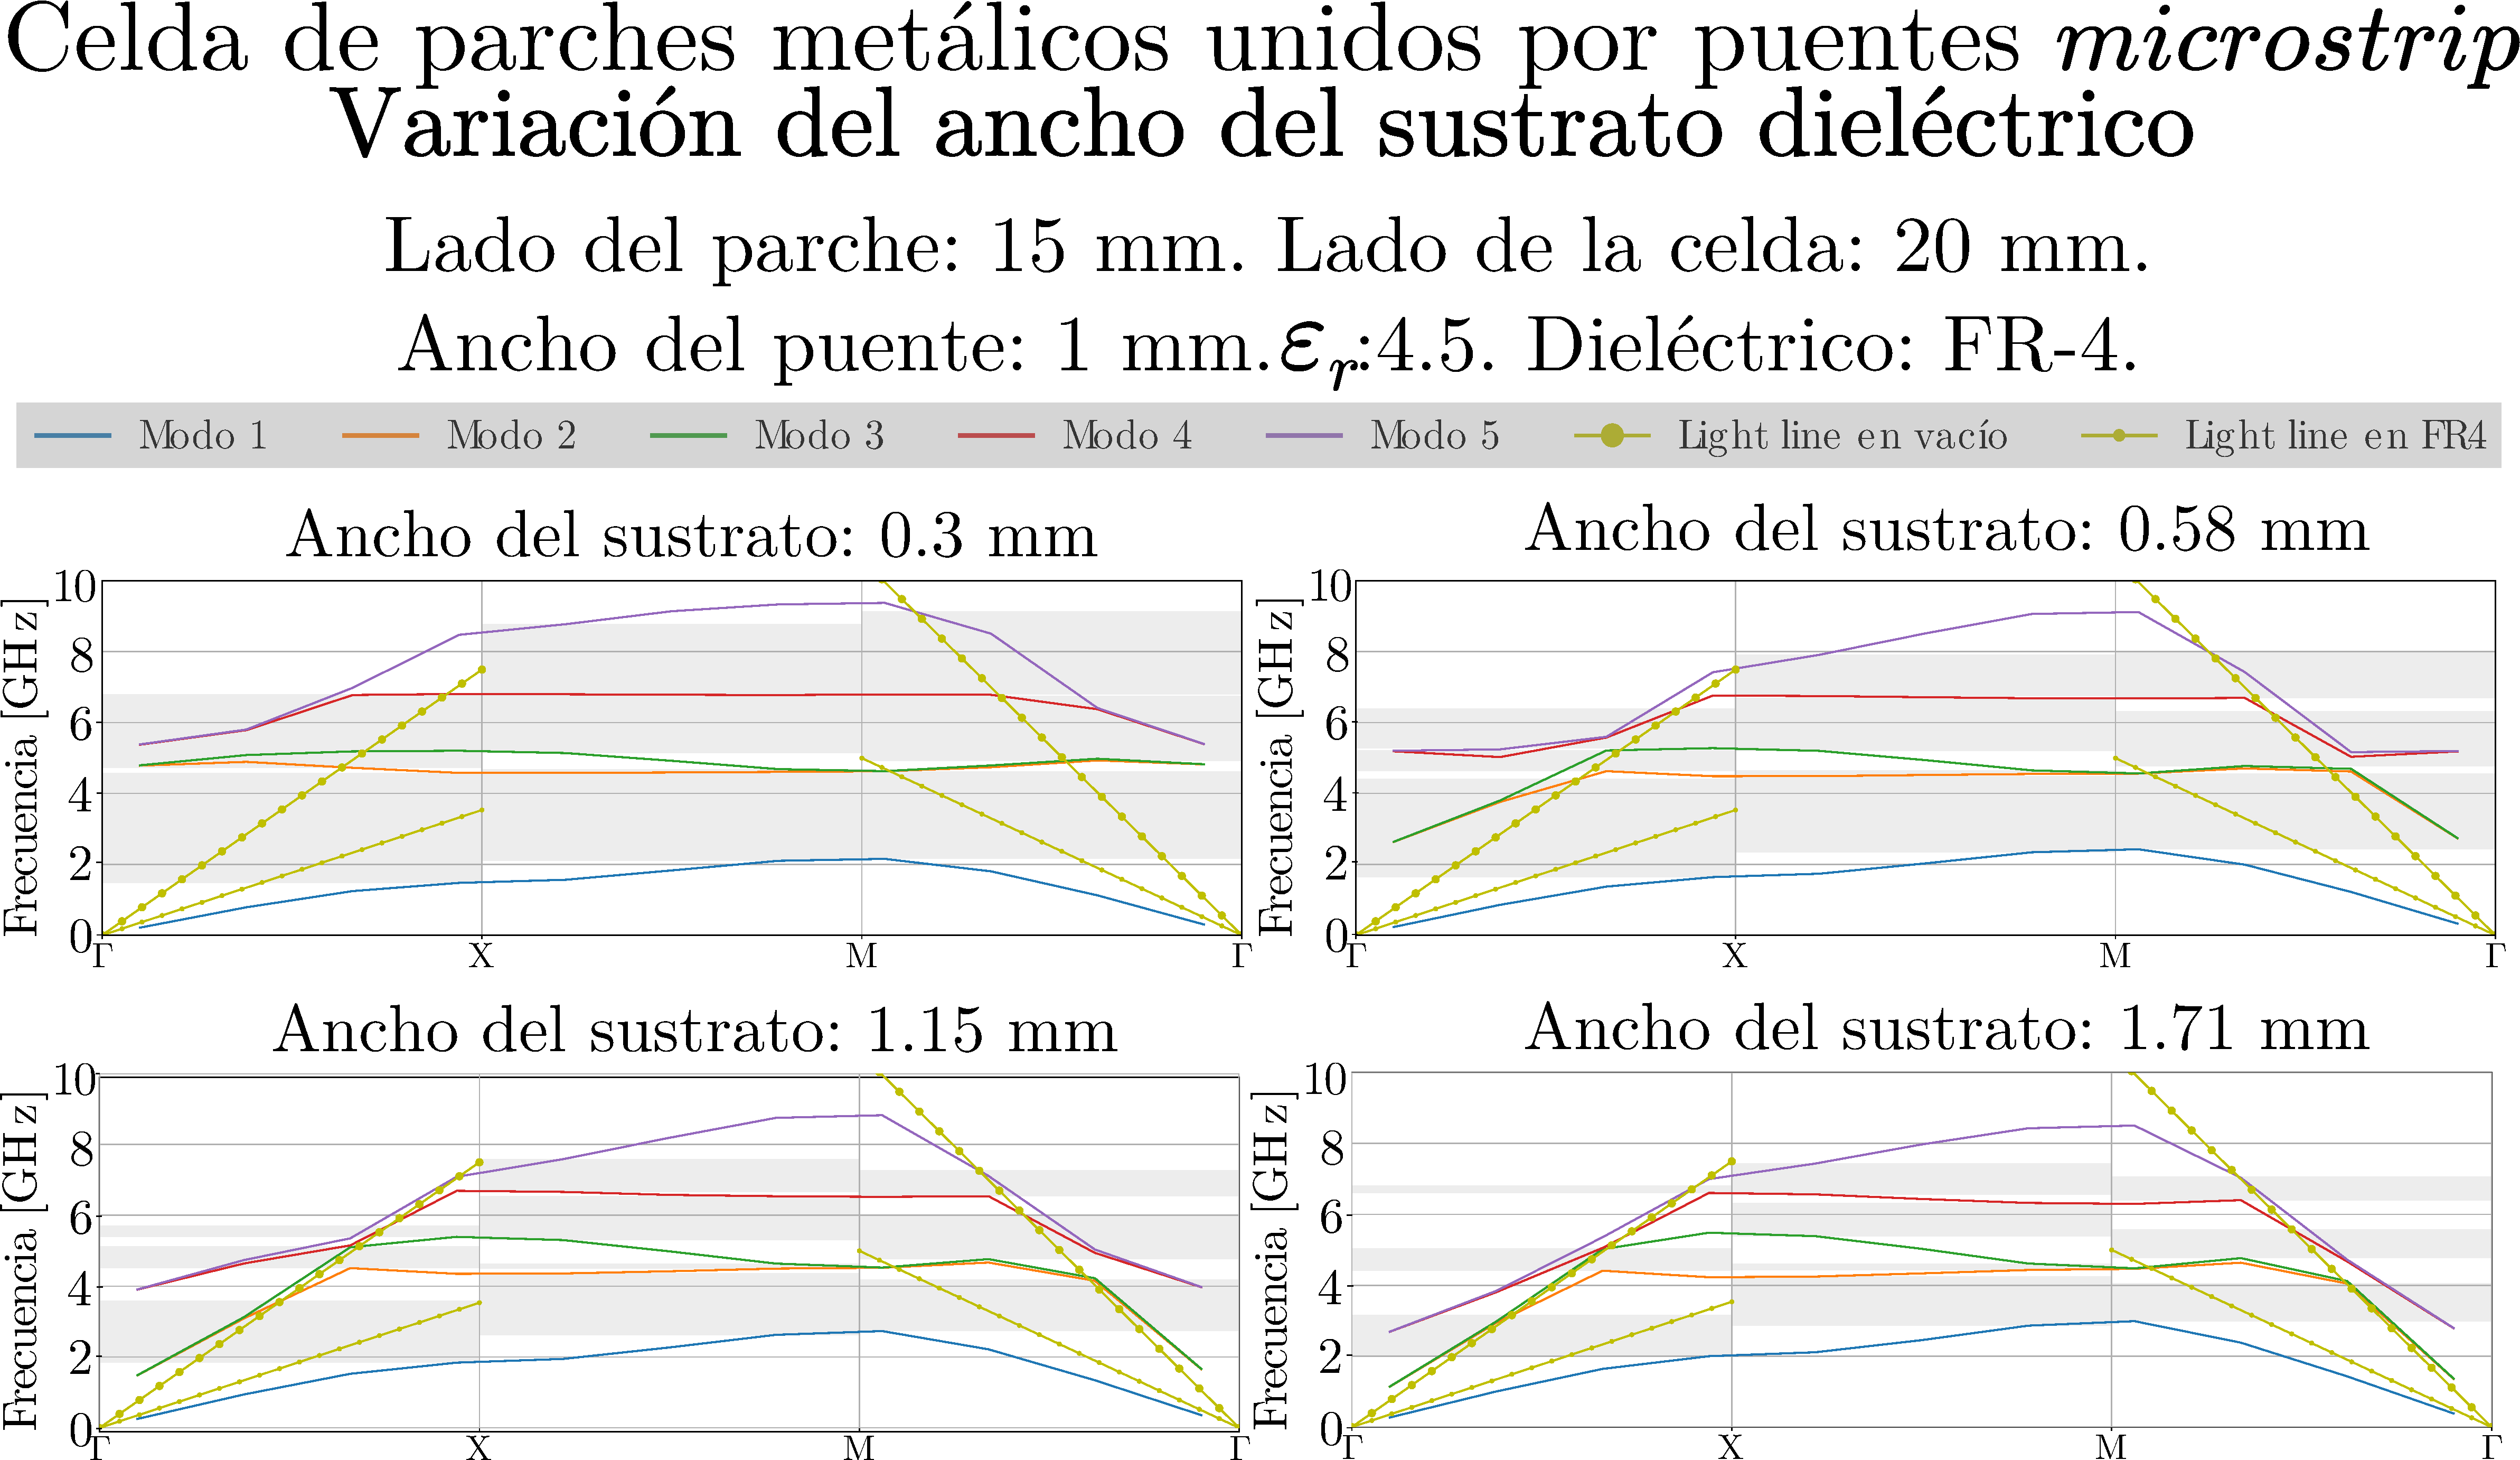
\includegraphics[width=1\textwidth]{Modelado/Orlandi-DeltaAnchoSustrato.pdf}
	\caption{Diagramas de dispersión para la variación del ancho del sustrato dieléctrico. El sustrato de FR-4 de $1.6\;\text{mm}$ de espesor.}
	\label{fig:diagdisp-orlandi-variacion-ancho-diel}
\end{figure}


\begin{figure}[h]
	\centering
	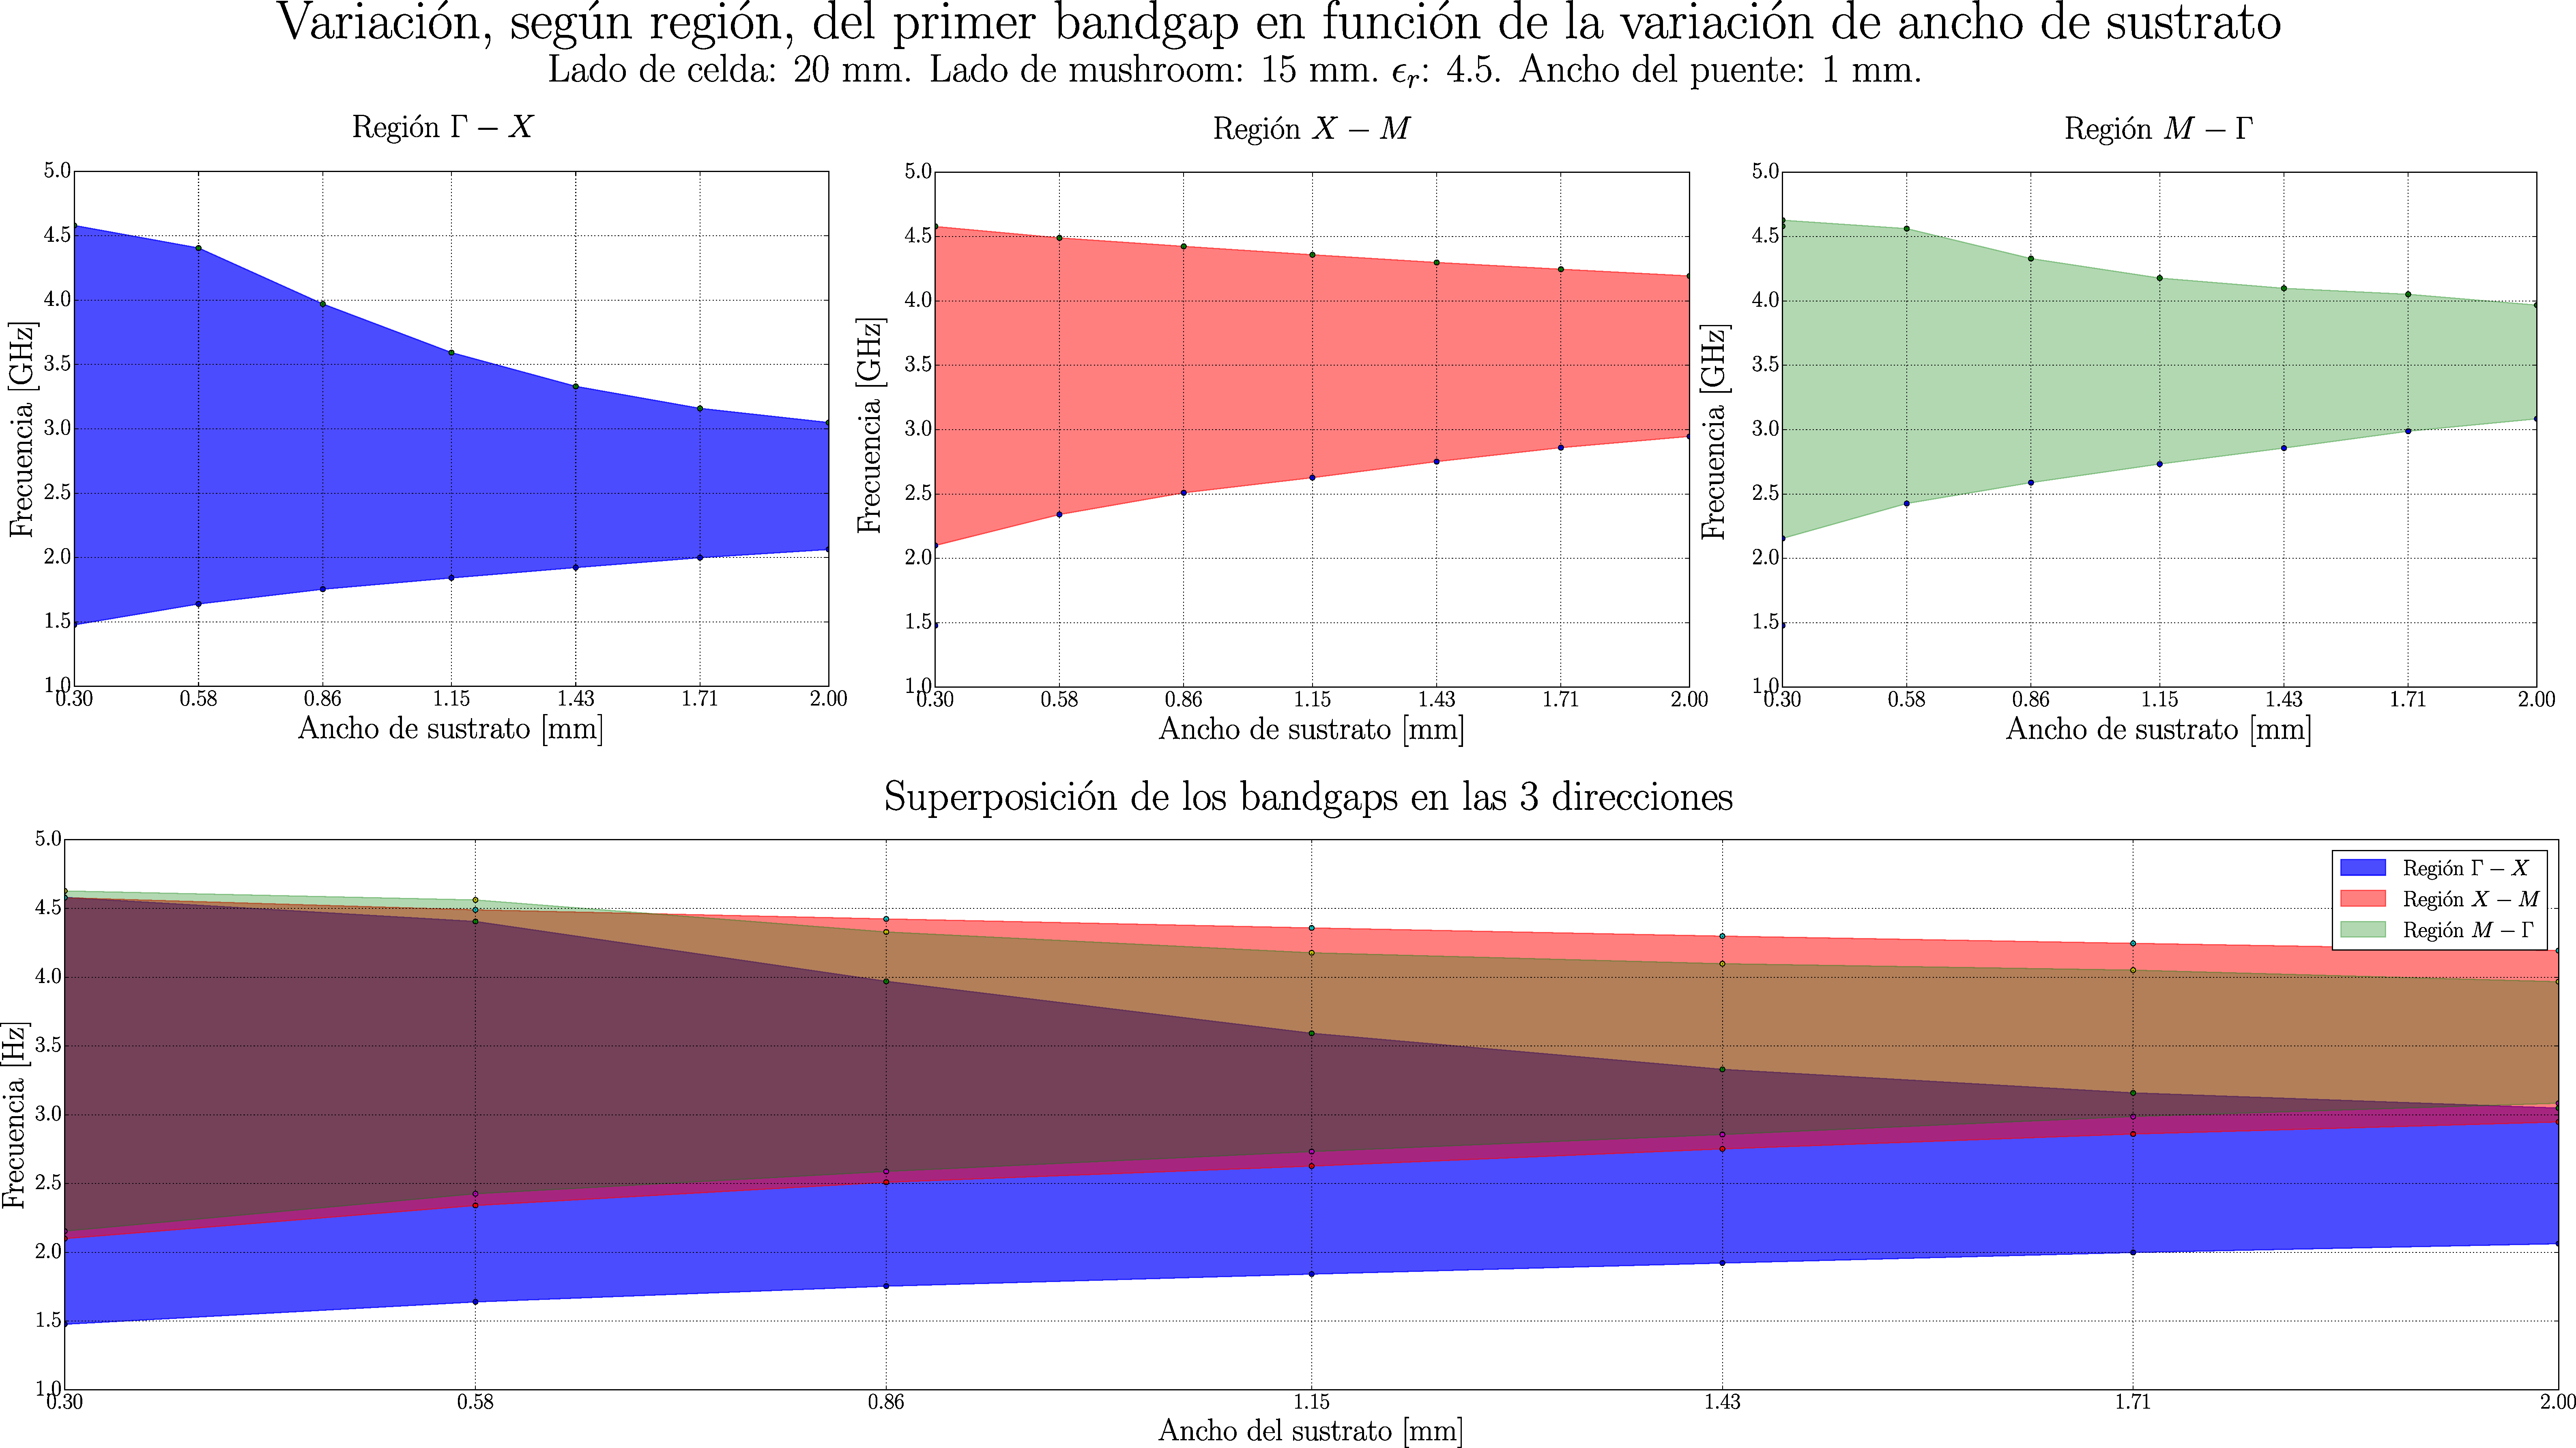
\includegraphics[width=1\textwidth]{Modelado/Orlandi-3direcciones-anchoSustrato-Comparacion.pdf}
	\caption{Comparación del ancho del primer band-gap (entre el primer y el segundo modo de propagación) para las tres direcciones analizadas, en función del ancho del sustrato dieléctrico.}
	\label{fig:comparacion-diagdisp-orlandi-variacion-ancho-diel}
\end{figure}

La variación del ancho del sustrato tiene importantes consecuencias en el EBG. Por un lado, es importante notar que el comportamiento del ancho de banda es opuesto al que se obtiene considerando el modelo cuasiestático: Un aumento en la capacidad (debido al acercamiento de los planos paralelos que forman los parches y el plano conductor inferior, cuando disminuye el ancho del sustrato), debería dar lugar a una disminución notoria en el ancho de banda. Sin embargo, como se observa en la figura \ref{fig:comparacion-diagdisp-orlandi-variacion-ancho-diel}, se da el efecto contrario.

El comportamiento resulta más intuitivo si se recuerda que, como se explicó en la sección \ref{cap_intro_electro}, un sustrato delgado dificulta la aparición de ondas de superficie, volviendo a las zonas prohibidas de propagación más notorias.

A medida que aumenta el tamaño del mismo, disminuye el ancho de banda de la zona prohibida, y resulta más dificultoso obtener un \textit{bandgap} completo.

\clearpage

\subsection{Celda de Yang}
\label{sec:celda-yang}

La búsqueda de estructuras que requirieran un menor tamaño de celda unitaria para lograr zonas prohibidas en frecuencias bajas, impulsó a Fei-Ran Yang, Kuang-Ping Ma, Yongxi Qian y Tatsuo Itoh, en 1991, a presentar \cite{Yang:UCPBG} la geometría mostrada en la figura \ref{fig:celda-yang}. En la misma, como se puede observar, se intentó maximizar la longitud de los puentes, estableciendo lo que se conoce como un \textit{inset} en el parche \textit{microstrip}. De esta forma, el parche puede crecer, y por tanto aumentar la capacidad, sin que por ello la inductancia deba disminuir. Esto permite, además, que los parches de las distintas celdas unitarias se ubiquen a corta distancia unos de otros, aumentando entonces el acoplamiento capacitivo entre ellos, y por tanto la capacidad del sistema completo. A pesar de las modificaciones, la simetría se mantuvo, por lo que las rectas de análisis de la zona irreducible de Brillouin son las mismas que para el caso de la celda analizada en la sección \ref{sec:celdas-orlandi}.

\begin{figure}[h]
	\centering
	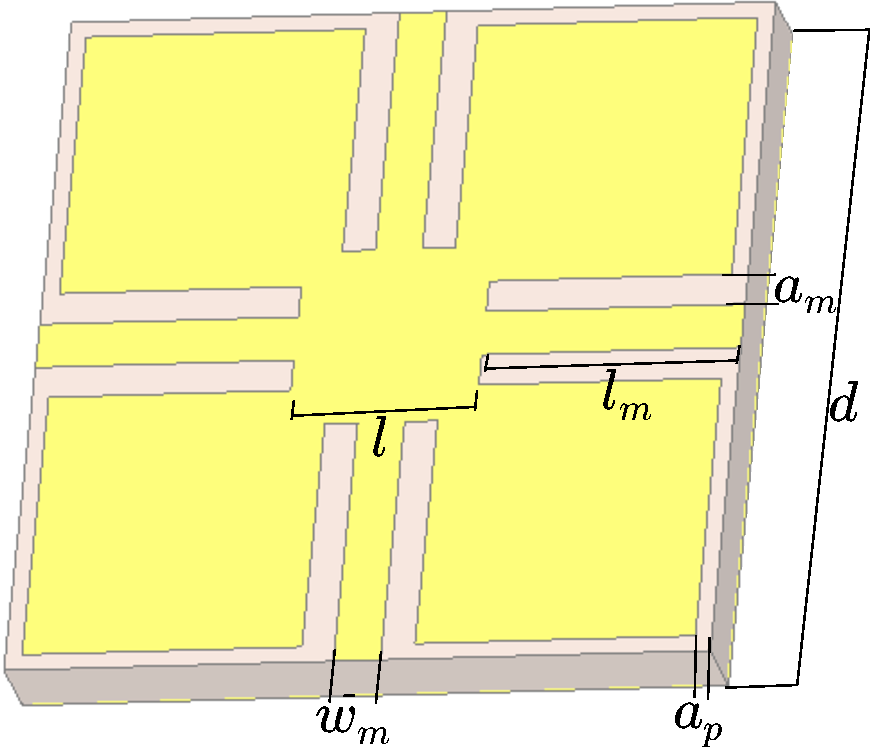
\includegraphics[width=0.4\textwidth]{Modelado/yang-celda.pdf}
	\caption{Celda unitaria del metamaterial presentado en 1999 por Yang, Ma, Qian e Itoh.}
	\label{fig:celda-yang}
\end{figure}

Aplicando, nuevamente el análisis de autovalores con condiciones de borde periódicas, se puede observar el comportamiento de los campos, más complejo que en la celda unitaria analizada antes. El mismo se muestra en la figura \ref{fig:yang-analisis-campos}.

Para el primer modo de propagación, resuelta evidente que, como en la estructura de parches cuadrados unidos por puentes analizada antes, el campo eléctrico es principalmente normal al plano sobre el que se ubica la estructura, y se ubica mayormente bajo el parche, donde se presenta el efecto de placas planas paralelas. Sin embargo, debido  a que ahora los puentes parten desde el interior del parche, existen también componentes tangenciales a la superficie. Estas componentes, como se puede observar en la figura \ref{fig:yang-analisis-campos} b) (para el primer modo) y f) (para el segundo modo), son muy notorias en los bordes de la celda unidad, por lo que los efectos de acoplamiento capacitivo mutuo entre celdas son mucho más notorios que en la celda analizada antes.

\begin{figure}[h]
	\centering
	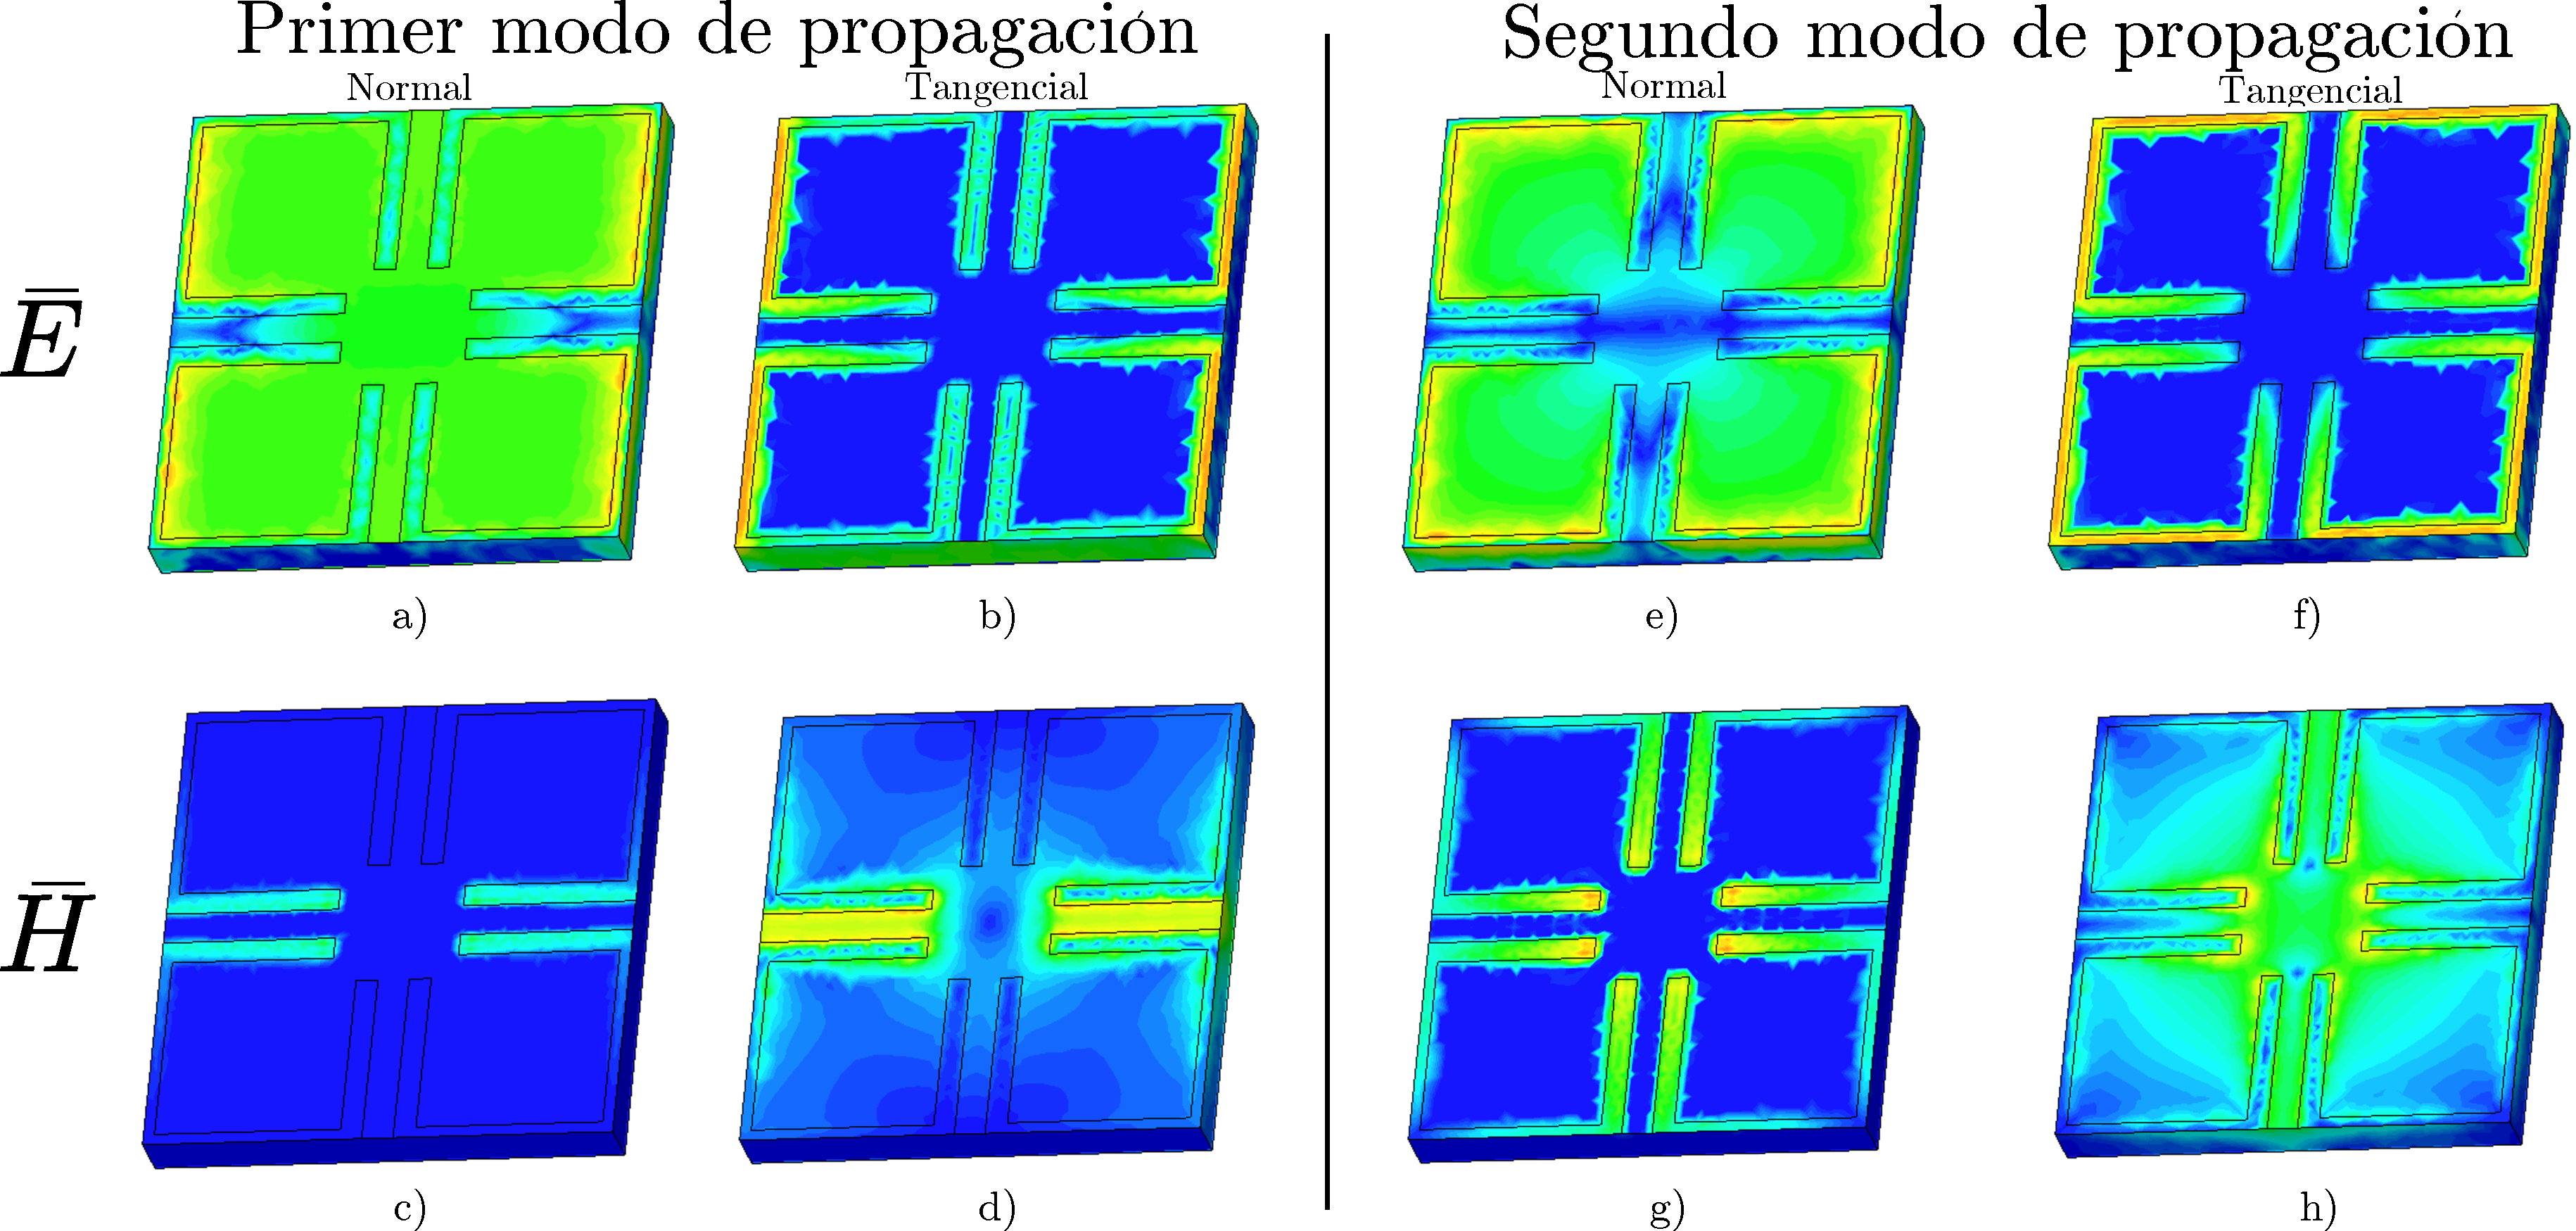
\includegraphics[width=1\textwidth]{Modelado/yang-modo1-Enorma-Etangencial.pdf}
	\caption{Comportamiento, en promedio temporal, de los campos eléctrico y magnético sobre una celda unitaria de Yang, para el primer y segundo modo de propagación.}
	\label{fig:yang-analisis-campos}
\end{figure}

Los campos magnéticos, por otro lado, para el primer modo de propagación son muy similares a los que presenta la celda analizada antes, incluyendo su variación temporal, que puede verse en las figuras \ref{fig:yang-analisis-campos-fases} c) y d) para dos tiempos distintos dentro del periodo. En el primero de ellos, cuando el campo eléctrico tiene amplitud máxima sobre el parche (figura a)), la corriente saliente al parche a través de los puentes horizontales crece. De la misma forma, cuando la tensión en el parche decrece a su mínimo, la corriente entrante al parche es máxima.

Para el segundo modo de propagación, el campo eléctrico, en promedio (figura \ref{fig:yang-analisis-campos} e) y f)) tiene un comportamiento muy similar al primer modo de propagación, pero como se puede observar en las figuras correspondientes de la figura \ref{fig:yang-analisis-campos-fases}, para tiempos distintos, el campo es mayor, alternadamente, en la parte superior e inferior de los parches. El campo magnético normal a superficie, en promedio, se puede observar, para este modo de propagación, presente en todas las aperturas metálicas de la celda unidad, indicando que sobre los parches y los bordes del parche circula una corriente notoria. En las figuras \ref{fig:yang-analisis-campos-fases} g) y h) se puede observar el campo magnético para dos momentos de tiempo distinto. Este campo magnético sugiere que en los puentes horizontales hay corrientes en ambas direcciones en todo momento (debido a que las dos aperturas que lo rodean presentan un campo magnético normal saliente), mientras que los puentes verticales poseen corrientes en un único sentido y, al contrario que para el caso de los puentes horizontales del primer modo, en este caso el sentido es el mismo.

\begin{figure}[h]
	\centering
	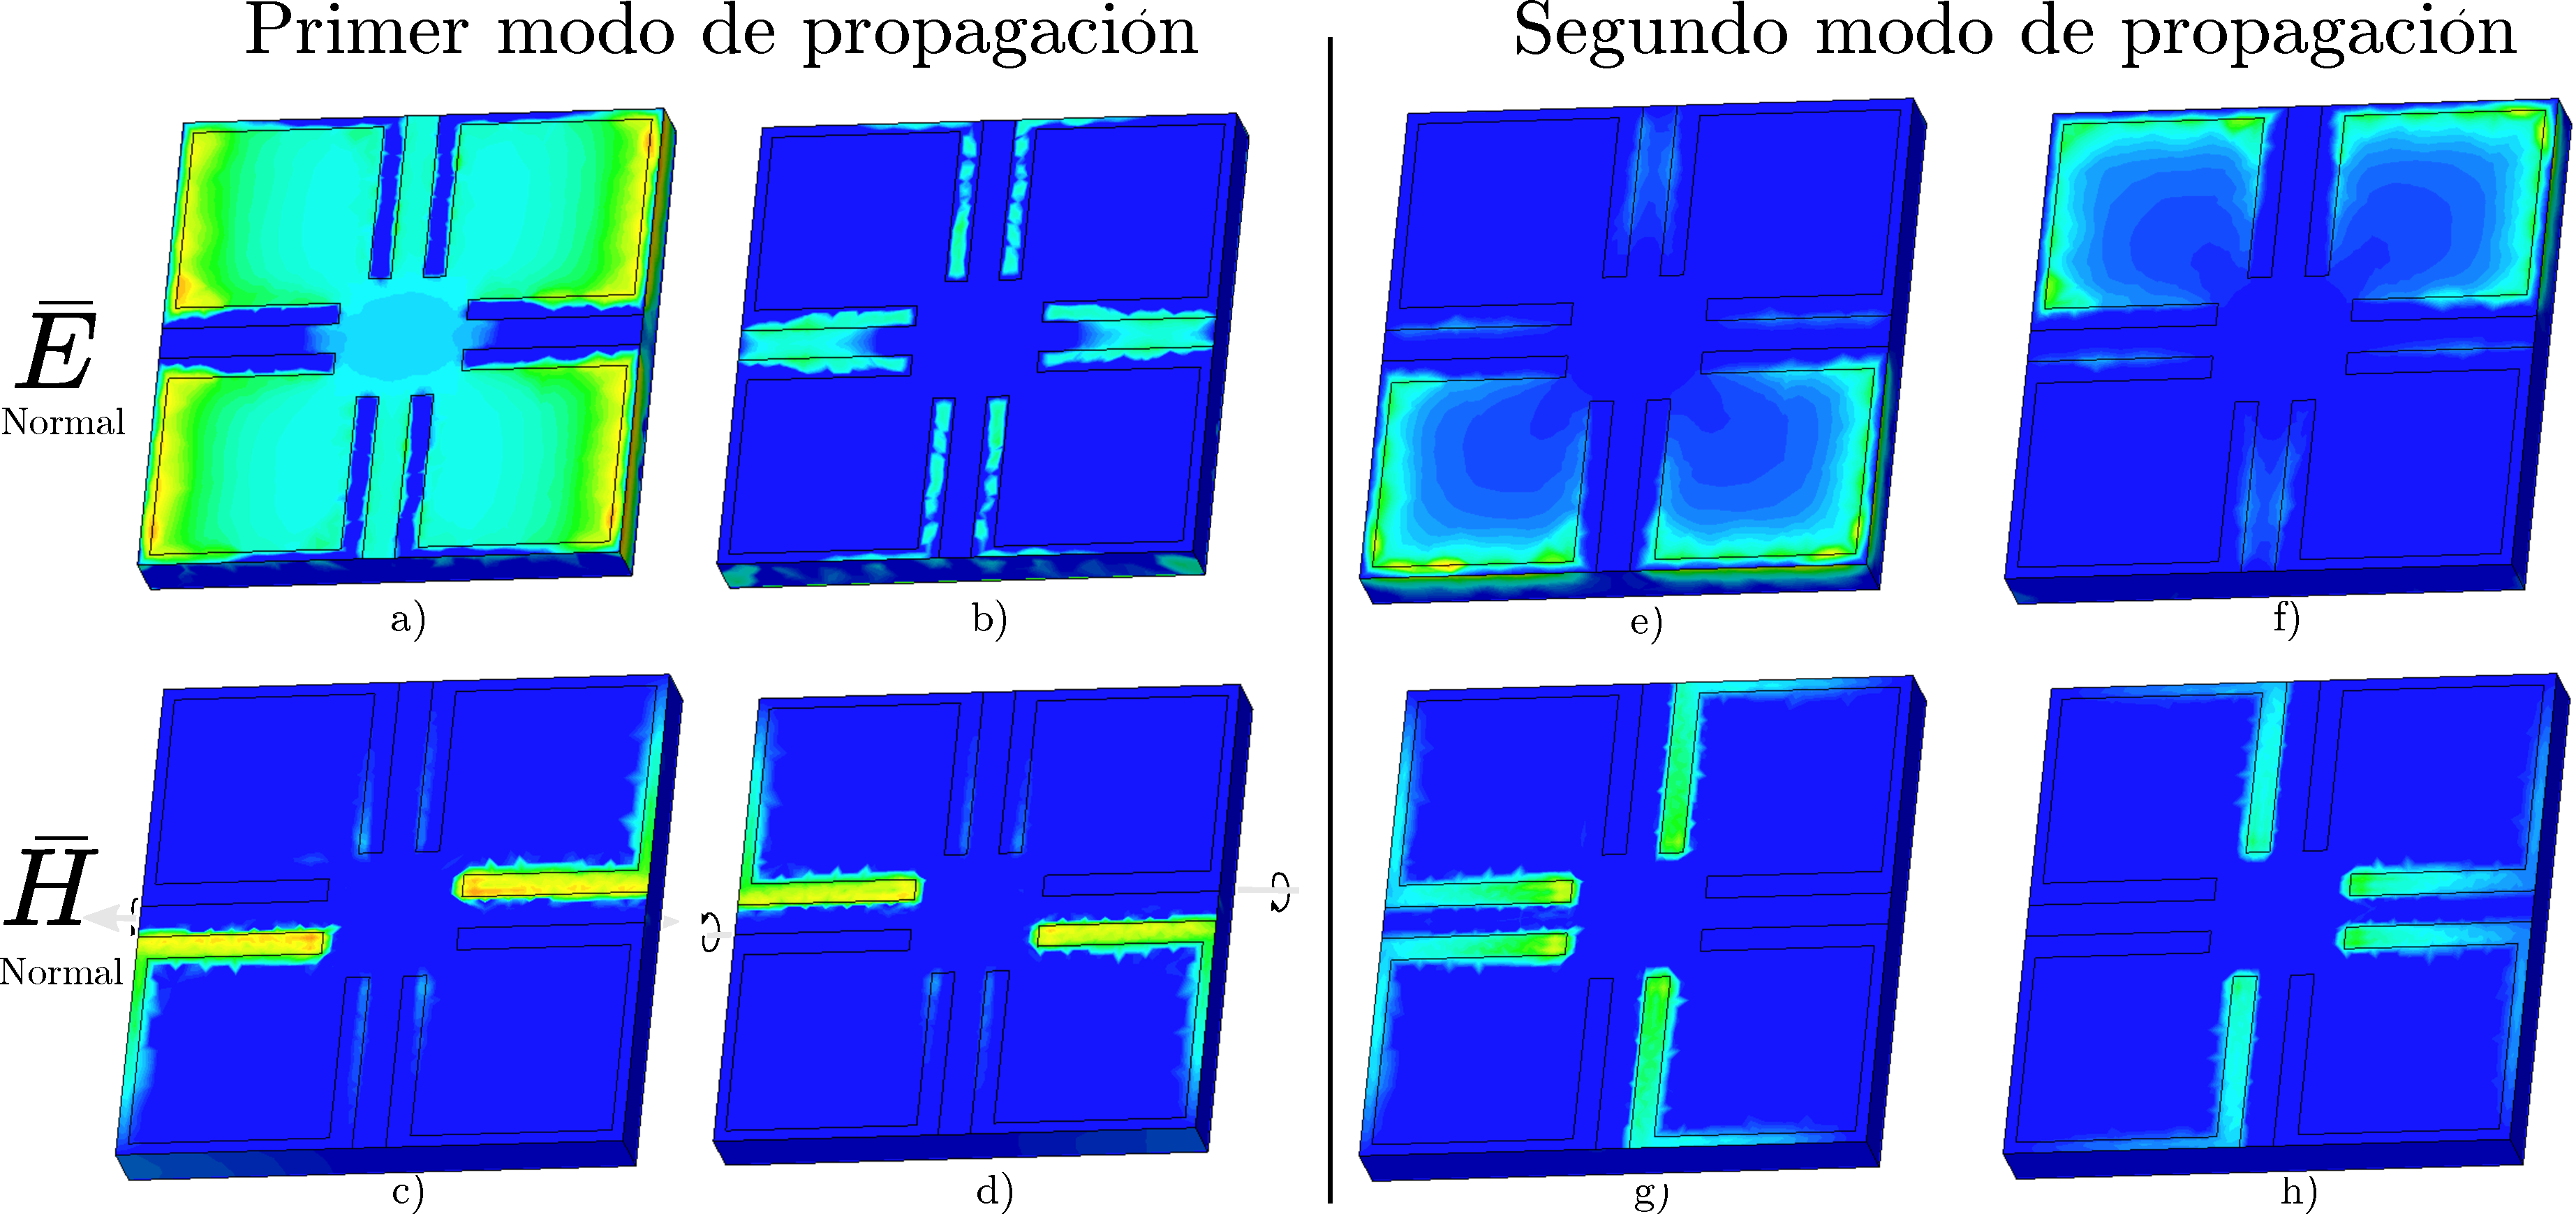
\includegraphics[width=1\textwidth]{Modelado/yang-modo1-EH-fases.pdf}
	\caption{Comportamiento, para dos tiempos diferentes, de los campos eléctrico y magnético normales a la superficie, sobre la celda propuesta por Yang, Ma, Qian e Itoh, para el primer y segundo modo de propagación.}
	\label{fig:yang-analisis-campos-fases}
\end{figure}


Se debe tener en cuenta que el uso de esta estructura presenta mayores dificultades, especialmente cuando su construcción se realiza por técnicas rudimentarias. Sin embargo, gracias a un mejor aprovechamiento del espacio, que permiten obtener una mayor capacidad e inductancia por celda unitaria, la geometría permite diseñar celdas unitarias más pequeñas para lograr zonas prohibidas para frecuencias de microondas que las que se pueden lograr utilizando la geometría analizada en la sección \ref{sec:celda-orlandi}.

\section{Modelado circuital}

La forma más sencilla de modelar el comportamiento resonante es la representación circuital, como la discutida en la sección \ref{sec:modelo_analitico}. En la misma deben intervenir capacitores e inductores con valores seleccionados en función del comportamiento de la energía en la estructura. Si bien los efectos de altas frecuencias no podrán ser analizados bajo esta representación, sí debería ser posible observar, al menos en forma general, los fenómenos analizados para las frecuencias de trabajo, de manera que se pueda abordar el problema intuitivamente.

Para el caso particular de la celda de Yang presentada en la sección \ref{sec:celda-yang}, a raíz del análisis del comportamiento de los campos, resulta fácil comprender que, si bien los fenómenos que intervienen son numerosos, los más importantes están fuertemente vinculados a la circulación de corriente por el puente y al desarrollo del campo eléctrico entre las celdas.

Se propusieron distintos circuitos, de diversa complejidad, para representar a cada celda unitaria propuesta por Yang, basados principalmente en el circuito mostrado en la figura \ref{fig:circuito-equivalente-kim-parches} y se analizaron los parámetros $S_{21}$ de cada uno, en vistas de lograr un comportamiento similar al obtenido cuando se utiliza el software \textit{CST Microwave Studio} para simular la estructura. El primero de los circuitos propuestos se puede observar en la figura \ref{fig:primerCircuitoPropuesto}, junto con los parámetros geométricos que dan lugar a los valores de los componentes circuitales. En el mismo se intentó utilizar la estructura LC paralela resonante para obtener un \textit{bandgap} para el rango de frecuencias estudiado.

\begin{figure}[h]
	\centering
	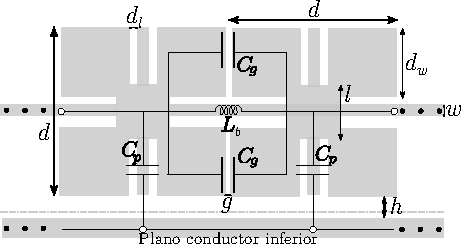
\includegraphics[width=1\textwidth]{Fundamentos/circuito-equivalente-celda-YANG-2.pdf}
	\caption{Primer circuito equivalente propuesto, con LC paralelo para obtener efecto \textit{notch}.}
	\label{fig:primerCircuitoPropuesto}
\end{figure}

La estructura LC paralela posee una frecuencia de resonancia en $f=1/(2 \pi \sqrt{LC})$, en la que abandona su comportamiento inductivo, y adopta uno predominantemente capacitivo. Para esa frecuencia, existe un intercambio de energía entre el inductor y el capacitor, de forma que la impedancia de entrada presenta un máximo. A esta frecuencia, entonces, el circuito se comporta como un filtro de tipo \textit{notch}, que podría explicar parte del comportamiento de \textit{bandgap} en microondas.

Por otro lado, la existencia de una capacidad de las celdas contra el plano de tierra da lugar, al menos para las bajas frecuencias, a un comportamiento pasabajos, debido a la relación entre los componentes $L_b$ y $C_p$.

Los valores geométricos de la celda unitaria utilizada como testigo son los que se muestran en la tabla \ref{table:CeldaUnitariaAnalisisiCircuital}, en función de los valores descriptos en la figura \ref{fig:primerCircuitoPropuesto}. Se consideró la permitividad relativa del FR-4, de $4.4$.

\begin{table}
	\centering
	\begin{tabular}{|c|c|c|c|c|c|c|}
		
		\hline
		$d$ & $l$ & $w$ & $d_l$ & $g$ & $h$ & $d_w$\\ 
		\hline
		$22.6\;mm$ & $6\;mm$ & $1.1\;mm$ & $0.8\;mm$ & $0.8\;mm$ & $1.6\;mm$ & $16.6\;mm$\\ 
		\hline 
	\end{tabular}
	\caption{Valores geométricos de la celda unitaria analizada.}
	\label{table:CeldaUnitariaAnalisisiCircuital}
\end{table}

La inductancia parcial del puente, $L_b$, se obtiene en base a 3 cálculos independientes, provenientes de modelos distintos de comportamiento de estructuras \textit{microstrip}. El primero de ellos es el mostrado en la ecuación \ref{eq:cgap-y-lgap}, repetido en la ecuación \ref{eq:lbridge1-circuital} por comodidad.

\begin{equation}
\label{eq:lbridge1-circuital}
L_{b} = 0.2\; \text{nH/mm} \cdot \ln \left(2\pi \frac{h}{w}\right).
\end{equation}

El segundo método es el propuesto por C. Paul en \cite{CPaul:InductanceLoopAndPartial}:

\begin{equation}
\label{eq:lbridge2-circuital-cpaul}
L_{b} = \begin{cases}
			\frac{60 l}{c} \ln \left( \frac{8h}{w} + \frac{w}{4h} \right) \text{ para } \frac{w}{h}\leq 1\\
			\frac{120 \pi l}{c} \frac{1}{w/h+1.393+0.667\ln(w/h+1.444)} \text{ para } \frac{w}{h} > 1 \\
		\end{cases}
\end{equation}

Por último, la inductancia parcial se calculó utilizando el software \textit{Ansys Q3D Extractor} de \textit{Ansoft}, que realiza simulaciones cuasiestáticas utilizando el método BEM (\textit{Boundary Element Method}), basado en la resolución de las funciones de Green, y que por lo tanto sólo requiere la discretización de la fuente de campo, y no del espacio circundante.

Los valores de $L_b$ obtenidos se muestran en la tabla \ref{table:Lb}.

\begin{table}
	\centering
	\begin{tabular}{|c|c|c|}
		\hline 
		Método 1 & Método 2 & Método 3\\ 
		\hline 
		$7.34\;nH$ & $8.2\;nH$ & $7.7\;nH$\\ 
		\hline 
	\end{tabular}
	\caption{Valores de inductancia de puente $L_b$ calculados por distintos métodos.}
	\label{table:Lb}
\end{table}

El valor de la capacidad entre las protuberancias de las celdas unitarias, $C_g$, se calculó utilizando la expresión de la ecuación \ref{eq:lbridge1-circuital}, repetida aquí por comodidad, y bajo la nomenclatura del problema:

\begin{equation}
\label{eq:cgap1-circuital}
C_{g} = \frac{d_w\epsilon_0(1+\epsilon_r)}{\pi}\cosh^{-1}\left(\frac{2 d_w + g}{g}\right).
\end{equation}

Además, se utilizó también \textit{Q3D Extractor} para obtener un valor aproximado de capacidad entre dos celdas unitarias, utilizando la geometría mostrada en la figura \ref{fig:capacidad-cg-Q3D}. Se consideró, tanto en la ecuación \ref{eq:cgap1-circuital} como en la simulación, que la principal responsabilidad por la capacidad entre celdas vecinas recae sobre las esquinas más próximas de las celdas unitarias. Además, para la simulación fue necesario eliminar el puente \textit{microstrip} que las conectaba, debido a que, dado que la simulación es cuasiestática, si el conductor es el mismo, la capacidad resulta nula.

\begin{figure}[h]
	\centering
	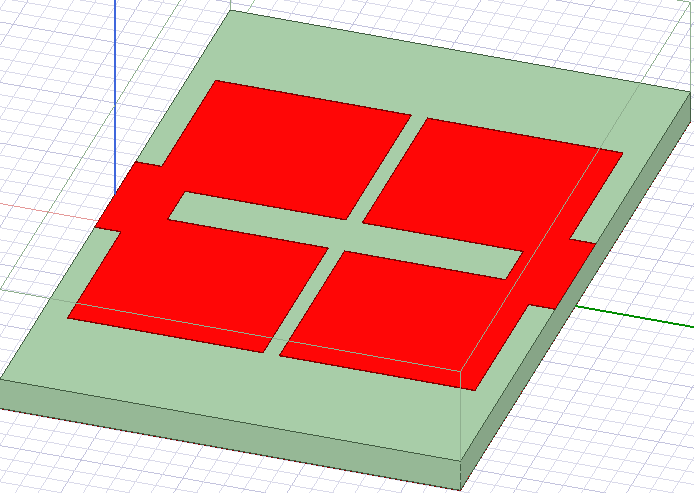
\includegraphics[width=0.5\textwidth]{Modelado/capacidad-cg-Q3D.png}
	\caption{Geometría utilizada para calcular la capacidad entre celdas vecinas con Q3D Extractor.}
	\label{fig:capacidad-cg-Q3D}
\end{figure}

\begin{table}
	\centering
	\begin{tabular}{|c|c|}
		\hline 
		Aproximación matemática & Simulación \\ 
		\hline 
		$475 fF\;$ & $130 fF$\\ 
		\hline 
	\end{tabular}
	\caption{Valores de capacidad de \textit{gap} calculados por distintos métodos.}
	\label{table:Cg}
\end{table}

Se observa que los valores son disimiles entre sí, por lo que, en el circuito, el valor de esta capacidad deberá ser obtenido por deducción en base al comportamiento en frecuencia, manteniendo estos valores como referencia o cotas aproximadas.

Finalmente, la capacidad contra el plano de tierra, $C_p$ se calculó utilizando la noción de capacitor de placas planas paralelas, debido a la corta distancia entre las celdas unitarias y el plano de tierra (según la tabla \ref{table:CeldaUnitariaAnalisisiCircuital}, $h=1.6\;mm$). El área total resulta:

\begin{align}
	Sup &= l^2+4 d_w^2+4 \frac{d-l}{2} w - 4 \left(\frac{l-w-2 d_l}{2}\right)^2 \\
	C_{p} &= \frac{Sup\; \epsilon_0 \epsilon_r}{h}
\end{align}

Además, se utilizó el software de simulación \textit{Q3D Extractor} para obtener un resultado comparativo. Los resultados se muestran en la tabla \ref{table:Cp-modelo1-circuital}, en donde se observa que la aproximación de placas planas paralelas ofrece un valor cercano al simulado utilizando BEM, incluso cuando no considera los efectos de \textit{fringing} en los bordes.

\begin{table}
	\centering
	\begin{tabular}{|c|c|c|}
		\hline 
		Superficie & Cálculo analítico & Q3D Extractor\\ 
		\hline 
		$458\; mm^2$ & $11.14\;pF$ & $12.26\;pF$\\ 
		\hline 
	\end{tabular}
	\caption{Valores de capacidad $C_p$ calculados por distintos métodos.}
	\label{table:Cp-modelo1-circuital}
\end{table}

Tras la estimación de los valores circuitales correspondientes, se debe analizar el comportamiento del parámetro $S_{21}$ de la estructura, para estudiar el efecto de atenuación. El mismo se muestra en la figura \ref{fig:s21-modelo1}, donde se grafica, además, el comportamiento de este parámetro según simulaciones de onda completa realizadas con \textit{CST Microwave Studio}, utilizando FEM (\textit{Finite Elements Method}), que es un método numérico en el dominio de la frecuencia. Como resultaba previsible, la frecuencia de resonancia cumple, al menos en forma aproximada (sin considerar más efectos que los expuestos hasta el momento) que $1.8\;GHz \approx 1/(2\pi\sqrt{L_{b} 2C_{g}}) \leq 3.75 \;GHz $, según los máximos y mínimos valores posibles de $L_b$ y $C_g$ mostrados en las tablas \ref{table:Lb} y \ref{table:Cg} respectivamente.

\begin{figure}[h]
	\centering
	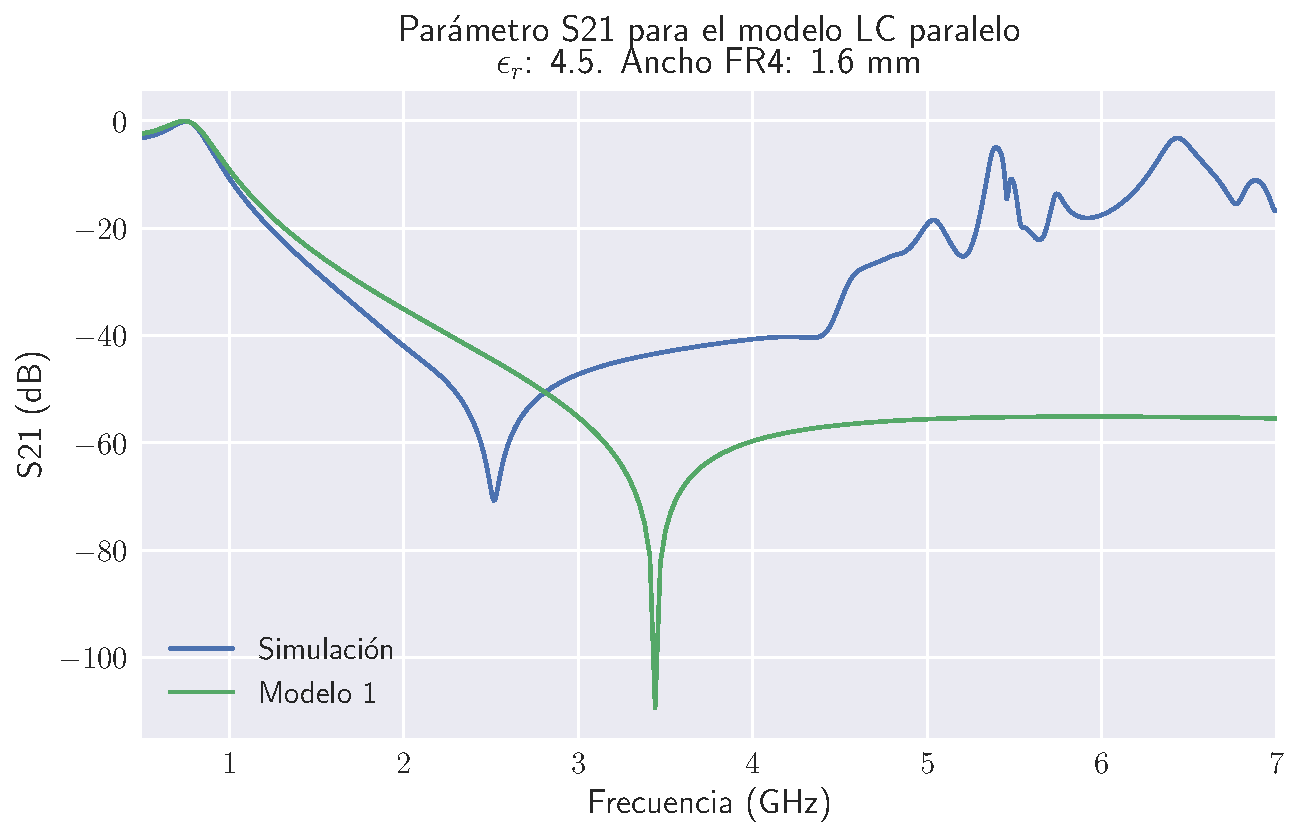
\includegraphics[width=1\textwidth]{Modelado/3-4.pdf}
	\caption{Comportamiento del parámetro $S_{21}$ para el modelo 1.}
	\label{fig:s21-modelo1}
\end{figure}

Como se puede observar, el comportamiento del modelo circuital difiere del obtenido mediante la simulación de onda completa, en particular en lo que respecta a la posición de la frecuencia de resonancia y al comportamiento en altas frecuencias, donde resulta esperable que el \textit{bandgap} ya no sea observable.

Bajo estas consideraciones, resulta menester considerar más condiciones que las seleccionadas inicialmente, nuevamente en base al circuito \ref{fig:circuito-equivalente-kim-parches}. Si se asume que las esquinas presentan una inductancia que no resulta despreciable, la misma resonará en serie con el capacitor $C_g$, imponiendo una menor impedancia para un rango de frecuencias, habilitando un camino de corriente, y mejorando la transferencia a través de la celda unitaria, lo que efectivamente limitaría el ancho de banda del \textit{bandgap}. El circuito propuesto se muestra en la figura \ref{fig:modelo-circuital-con-lw}. 

\begin{figure}[h]
	\centering
	\includegraphics[width=1\textwidth]{Fundamentos/circuito-equivalente-celda-YANG-6.pdf}
	\caption{Segundo circuito equivalente propuesto.}
	\label{fig:modelo-circuital-con-lw}
\end{figure}

Si de esta estructura sólo se analiza intuitivamente el fenómeno de resonancia serie, se puede trabajar sobre el circuito mostrado en la figura \ref{fig:p13-p14-sdf} a), cuya gráfica de parámetro S12 se observa en la figura \ref{fig:p13-p14-sdf} b). Para el caso graficado, la frecuencia de resonancia serie se ubica en aproximadamente $6\; GHz$, donde se manifiesta el efecto descripto.

\begin{figure}[H]
	\centering 
	\subfigure[Circuito equivalente considerando sólo el efecto de la resonancia serie.]{
		\label{fig:modelo-circuital-resonancia-serie-p13-p14}
		\includegraphics[width=0.50\textwidth]{Fundamentos/circuito-equivalente-celda-YANG-3.pdf}}
	\hspace{0pt}
	\subfigure[Parámetro $S_{21}$ considerando resonancia serie únicamente.]{
		\label{fig:modelo-circuital-resonancia-serie-p13-p14-s12}
		\includegraphics[width=0.45\textwidth]{Modelado/13-14.pdf}}
	\caption{Análisis de la resonancia serie.}
	\label{fig:p13-p14-sdf}
\end{figure}

El valor de la inductancia que imponen los parches de las esquinas se calculó de tres formas. La primera se basa en el uso de la expresión de la inductancia de la ecuación \ref{eq:Cp_Lp}. La segunda consiste en el uso de las ecuaciones presentadas en \ref{eq:lbridge2-circuital-cpaul}. Finalmente, además, se realizaron simulaciones utilizando Q3D Extractor, para validar el uso de las expresiones. Los resultados se muestran en la tabla \ref{table:lw}. Resulta importante, sin embargo, señalar que, si bien la inductancia es un parámetro puramente geométrico, las posiciones de los puertos de entrada y salida modifican su valor. Estas posiciones no son tenidas en cuenta en las expresiones propuestas por la literatura, pero se las considera lo suficientemente cercanas al valor final.

\begin{table}
	\centering
	\begin{tabular}{|c|c|c|}
		\hline 
		Según expresión \ref{eq:Cp_Lp} & Según expresión \ref{eq:lbridge2-circuital-cpaul} & Q3D Extractor \\ 
		\hline 
		$2\;nH$ & $1.55\;nH$ & $4\;nH$\\ 
		\hline 
	\end{tabular}
	\caption{Valores de inductancia $L_w$ calculados por distintos métodos.}
	\label{table:lw}
\end{table}

La frecuencia de resonancia serie resulta, entonces, de

\begin{equation}
	f_r^{\text{serie}} = \frac{1}{2\pi \sqrt{C_g 2 L_w}},
\end{equation}

que, para los parámetros geométricos establecidos, varía entre $3.6\;GHz$ y $8\;GHz$. La amplitud de la incertidumbre se debe a la propia incertidumbre del valor la capacidad $C_g$.

Sin embargo, la aparición de estas nuevas inductancias $L_{w}$ modificará fuertemente la frecuencia de resonancia del circuito LC paralelo analizado antes. Para este nuevo circuito, la inductancia vista por sus terminales está dada por $L_{b}+2 L_{w}/2$, debido a que por los componentes circuitales correspondientes a las esquinas sólo circula la mitad de la corriente que lo hace por la inductancia central. El valor de la frecuencia de resonancia, entonces, debido al aumento de la inductancia equivalente, disminuye, para adoptar valores entre $1.4\;GHz$ y $2.6\;GHz$. Este mismo cambio de resonancia se observaría si las inductancias $L_w$ estuvieran dispuestas sobre la rama central, como se muestra en la figura \ref{fig:res-serie-p21p22}, lo cual valida el análisis, debido a que el hecho de que no estén en serie con los capacitores elimina el efecto de resonancia LC.

\begin{figure}[H]
	\centering 
	\subfigure[Circuito equivalente para el cálculo de la frecuencia de resonancia paralela, considerando las inductancias de las esquinas.]{
		\label{fig:modelo-circuital-resonancia-serie-p13-p14}
		\includegraphics[width=0.45\textwidth]{Fundamentos/circuito-equivalente-celda-YANG-7.pdf}}
	\hspace{0pt}
	\subfigure[Parámetro $S_{21}$ del circuito, comparado con el comportamiento mostrado en la figura \ref{fig:s21-modelo1}.]{
		\label{fig:modelo-circuital-resonancia-serie-p13-p14-s12}
		\includegraphics[width=0.45\textwidth]{Modelado/3-4-21-22.pdf}}
	\caption{Análisis del efecto sobre la resonancia LC paralelo de las inductancias de ala consideradas.}
	\label{fig:res-serie-p21p22}
\end{figure}

En la figura \ref{fig:modelo-circuital-resonancia-serie-graficos} se pueden observar que la composición de los dos efectos más importantes analizados hasta el momento (las resonancias serie y paralela) da lugar a un comportamiento similar a transferencia del circuito analizado.

\begin{figure}[h]
	\centering
	\includegraphics[width=1\textwidth]{Modelado/composicion.pdf}
	\caption{Superposición de los comportamientos de los circuitos analizados hasta el momento y la simulación obtenida con \textit{CST Microwave Studio}.}
	\label{fig:modelo-circuital-resonancia-serie-graficos}
\end{figure}


Queda aún por explicar el comportamiento de la transferencia entre las dos frecuencias de resonancia, donde los efectos no pueden considerarse fruto de la relación entre los elementos de un subconjunto del circuito. Resulta necesario tener en cuenta la inductancia que impone el parche central, análoga a la que imponen las esquinas de la celda unitaria. Esto obliga a que la capacidad de la celda unitaria no sea única y centralizada, como hasta el momento, sino que debe estar correctamente distribuida en la geometría: parte de la capacidad se debe al aporte de las esquinas, y otra parte al parche central. El circuito, más complejo, se muestra en la figura \ref{fig:modelo-circuital-todojunto-sinR}.

\begin{figure}[h]
	\centering
	\includegraphics[width=1\textwidth]{Fundamentos/circuito-equivalente-celda-YANG-5.pdf}
	\caption{Tercer circuito equivalente propuesto, considerando inductancias y capacidades distribuídas en la celda unitaria.}
	\label{fig:modelo-circuital-todojunto-sinR}
\end{figure}

Se puede observar que se agregaron las capacidades de las secciones de las esquinas ($C_w$), y se ubicaron en un nodo intermedio, entre la capacidad de gap $C_g$ y la capacidad del bloque central $C_c$, que ahora queda redefinida, dado que deja de representar a toda la superficie de la cara superior de la celda unitaria, para restringirse al cuadro central. Este cuadro, además, ahora presenta inductancia $L_c$. Además, se tuvo en cuenta la capacidad contra el plano de tierra del puente, $C_b$. Finalmente, se consideró el efecto de aquellas esquinas que no poseen una celda vecina, lo que aumenta la capacidad de la esquina (debido al efecto de \textit{fringe}) y la inductancia a considerar. Estos nuevos valores están representados por $C'_w$ y $L'_w$, y resultan importantes debido a que esta capacidad e inductancia resuenan a la frecuencia de interés, generando un camino de baja impedancia para la corriente y disminuyendo, por tanto, la transferencia.

El comportamiento del parámetro S21 se puede observar en la figura \ref{fig:s21-total-sin-R}. En la misma, se destaca que la frecuencia de resonancia, asi como los efectos para frecuencias cercanas a $6\; GHz$, se predicen adecuadamente, aunque no así los efectos de orden superior para esas frecuencias.

\begin{figure}[h]
	\centering
	\includegraphics[width=1\textwidth]{Modelado/69-70.pdf}
	\caption{Comportamiento del parámetro $S_{21}$ para el modelo propuesto, comparado a la simulación obtenida con \textit{CST Microwave Studio}.}
	\label{fig:s21-total-sin-R}
\end{figure}

Por último, resta considerar las pérdidas por conductividad y las pérdidas dieléctricas, para incorporarlas al circuito equivalente propuesto.

Las pérdidas por conductividad pueden ser representadas por una resistencia representando el comportamiento en corriente continua y otra en corriente alterna. Para la corriente continua, la resistencia que impone una cinta \textit{microstrip} depende de su largo $l$ y la superficie que es atravesada por el flujo, $S$. Para el caso de corriente alterna, debido al efecto \textit{skin} descripto en la ecuación \ref{eq:prof_penetacion}, se debe tener en cuenta la profundidad de penetración $\delta_s$, de manera que

\begin{align}
R_{dc} &= \frac{l}{\sigma S}, \\
R_{ac} &= \frac{l}{\sigma(2 w \delta_s+2 t \delta_s)} = \frac{l}{2\sigma \delta_s(w +t)} = \frac{l \sqrt{2 \pi f \mu \sigma}}{2 \sqrt{2}\sigma \delta_s(w +t)}, \\
R_s &= R_{dc} + R_{ac} = \frac{l}{\sigma} (\frac{1}{\sigma} + \frac{\sqrt{\pi f \mu \sigma}}{2 (w+t)})
\end{align}

donde $w$ es el ancho de la cinta \textit{microstrip} considerada, $t$ es su ancho vertical, y $f$ es la frecuencia a la que se desea encontrar la resistencia que modela el efecto en corriente alterna. El valor de la conductividad del cobre, $\sigma$, es de $5.7\;10^{-7}$.

Para el caso de las pérdidas dieléctricas, las pérdidas se representan como una conductancia $G$ dispuesta en paralelo a los capacitores que vinculan la capa superior de la celda unitaria con el plano de tierra.

Dicha conductancia puede ser calculada en base a la tangente de pérdidas del material, que es un parámetro ofrecido por el fabricante, y que fue definido en la ecuación \ref{eq:tan_perdidas}. El uso de una tangente de pérdidas asume la existencia de una impedancia imaginaria entre la capa superior y el plano de tierra en una celda unitaria, de manera que esta tangente representa la relación entre las partes real e imaginaria:

\begin{align}
	\tan(\delta) &= X/R = \frac{1/\omega C}{R} = \frac{G}{\omega C}, \\
	G &= \omega C \tan(\delta) = \frac{1}{R_p}
\end{align}

Para el caso de FR-4, la tangente de pérdidas posee el valor de 0.017.

El circuito final, considerando resistencias, se puede observar en la figura \ref{fig:modelo-circuital-todojunto-conR}.

\begin{figure}[h]
	\centering
	\includegraphics[width=1\textwidth]{Fundamentos/circuito-equivalente-celda-YANG-4.pdf}
	\caption{Circuito final equivalente propuesto, considerando inductancias y capacidades distribuídas en la celda unitaria, y resistencias de pérdidas.}
	\label{fig:modelo-circuital-todojunto-conR}
\end{figure}

Una comparación entre el comportamiento del parámetro $S_{21}$ considerando y sin considerar resistencias se puede observar en la figura \ref{fig:con-sin-R}.

\begin{figure}[h]
	\centering
	\includegraphics[width=1\textwidth]{Modelado/con-sin-R.pdf}
	\caption{Comportamiento del parámetro $S_{21}$ para el modelo propuesto, con y sin resistencias de pérdidas.}
	\label{fig:con-sin-R}
\end{figure}

Los valores finales de los parámetros utilizados para modelar la celda unitaria estudiada se muestran en la tabla \ref{table:valoresFinalesModelo}.

\begin{table}
	\centering
	\begin{tabular}{| c c | c c |}
		\hline 
		$L_b$ & $6.9\; nH$ & $C_g$ & $155\; fF$\\
		\hline
		$L_w$ & $1.9\; nH$ & $C_c$ & $1.24\; pF$ \\
		\hline
		$C_b$ & $378 \;fF$ & $C_w$ & $2 \; pF$\\
		\hline
		$C'_w$ & $2.372\; pF$ & $L'_w$ & $1.9\; nH$ \\
		\hline
		$R_{wp}$ & $936\; \Omega$ & $R_{ws}$ & $0.01\; \Omega$\\
		\hline
		$R_{bp}$ & $0.15\; \Omega$ & $R_{bs}$ & $4953\; \Omega$\\
		\hline
		$R_{cp}$ & $1509\; \Omega$ & $R_{cs}$ & $0.01\; \Omega$ \\
		\hline 
	\end{tabular}
	\caption{Tabla de valores finales elegidos.}
	\label{table:valoresFinalesModelo}
\end{table}

El comportamiento del parámetro $S_{21}$ según del modelo circuital se puede comparar al simulado utilizando \textit{CST Microwave Studio} en la figura \ref{fig:s12_modelo_final}.

\begin{figure}[h]
	\centering
	\includegraphics[width=1\textwidth]{Modelado/67-68.pdf}
	\caption{Comportamiento del parámetro $S_{21}$ para el modelo propuesto, comparado con el obtenido mediante simulación con \textit{CST Microwave Studio}.}
	\label{fig:s12_modelo_final}
\end{figure}

\section{Modelado por líneas de transmisión}
%%%%

Además del acercamiento a través del uso de circuitos equivalentes de primer orden, en general es posible expresar el problema a partir de su generalización como un conjunto de líneas de transmisión efectivas (en lugar de líneas de transmisión propiamente dichas), discretizando el espacio de forma que cada paso de discretización resulte mucho menor a $\lambda/4$ \cite{Caloz:ElectromagneticMetamaterials}, aproximadamente. Este acercamiento, y el uso de líneas de transmisión generalizadas (donde se pueden considerar capacidades en serie e inductancias en paralelo) resultan útiles para describir distintos tipos de metamateriales, incluyendo aquellos que son conocidos como ``de mano izquierda" \cite{Caloz:ElectromagneticMetamaterials}.

Para el caso bidimensional, la discretización debe ser también bidimensional, lo que conlleva mayores esfuerzos numéricos. Un problema práctico cualquiera puede contener una enorme cantidad de celdas unitarias, con bordes complejos y medios inhomogéneos, lo que obliga a considerar las propiedades de las celdas unitarias de la forma lo más sencilla posible, y para aumentar la densidad de las mismas con el menor impacto posible en el tiempo de procesamiento.

Existen numerosos métodos que utilizan líneas de transmisión para simular metamateriales, entre los que destacan el método de TMM (\textit{Transmission-Matrix Method}) y de TLM (\textit{Transmission-Line Matrix Method}). Si bien los nombres son similares, la resolución del problema varía fundamentalmente \cite{Caloz:ElectromagneticMetamaterials}. En este trabajo se desarrollará brevemente el método de TLM, que luego será implementado y explicado en detalle en la sección \ref{subsec_estudio_tlm}.

El método de matrices\footnote{Aquí el término matrices se refiere a un arreglo bidimensional, y no a un objeto matemático.} de líneas de transmisión consiste en la discretización espacial del problema físico en pequeñas subceldas. El comportamiento de los campos electromagnéticos en las mismas se concentra en un nodo o punto en el espacio, y las relaciones de adyacencia entre ellas se modelan utilizando líneas de transmisión que vinculan los nodos. Estas líneas son capaces de transmitir impulsos cortos sin distorsión, y de distribuirlos, en cada uno de los nodos, de acuerdo a un algoritmo local para cada subcelda \cite{Caloz:ElectromagneticMetamaterials}, hacia cada uno de los nodos adyacentes. Este algoritmo local no es más que la multiplicación del pulso incidente por los parámetros S de transmisión y reflexión en cada tiempo, que se pueden obtener a partir del análisis de la celda y sus vecinas. De esta manera, se discretiza un circuito equivalente al problema físico a resolver, y se simula la propagación de ondas electromagnéticas a partir del \textit{scattering} de impulsos en una red n-dimensional de nodos unidos por lineas de transmisión.

El algoritmo fue propuesto inicialmente en 1971 por Johns y Beurle \cite{JohnsBeurle:TLM}, y provee soluciones en el dominio del tiempo, a partir del estudio de la propagación de impulsos electromagnéticos muy cortos en las estructuras. La información en el dominio de la frecuencia se obtiene realizando una transformada de Fourier\footnote{Numéricamente, se suele realizar una transformada discreta de Fourier, cuya implementación más conocida es la Fast Fourier Transform (FFT)} de la respuesta de la red al impulso, como en todo método numérico en el dominio del tiempo. Esta metodología lo vuelve útil especialmente para aplicaciones de gran ancho de banda, donde se desea obtener características en un amplio rango de frecuencias con una única simulación.

El método fue generalizado, más tarde, al estudio de estructuras tridimensionales, donde se reemplazaron los conceptos de capacidad e inductancia de la línea de transmisión, por parámetros físicos del medio. En general, la capacidad e inductancia asociadas a las líneas de transmisión que unen los nodos que representan un medio en particular son elegidas de forma que la impedancia característica coincida con la impedancia intrínseca del mismo. En general, las pérdidas en el medio se tienen en cuenta a partir del uso de resistencias, o la aplicación de una constante de atenuación en cada cálculo de \textit{scattering} sobre los nodos.

% Cuentas! Wu, Lin, Wang, Wang, Chen

%%%%
\subsection{Algoritmo utilizando programación orientada a objetos}
\label{subsec_estudio_tlm}
%%%%
La simulación se corre a través de un \textit{script} editable de Python, donde se establecen las condiciones de la simulación en forma manual, y se determina si se leerán resultados calculados previamente o se calcularán nuevos. En el mismo, además, se permite elegir si se considerarán  las capacidades de acople entre elementos, la cantidad de tiempos a simular y las frecuencias superior e inferior de análisis. Se debe tener en cuenta, además, que se especifica la discretización espacial (cantidad de milímetros de cada estructura simulada, denominada \textit{Pixel}). La discretización espacial se relaciona con la temporal, dado que en TLM están vinculadas por la velocidad de propagación de una onda electromagnética en el medio. Así, la primera deberá asegurar que la segunda permita cumplir con las condiciones del teorema de Nyquist para la caracterización de las señales calculadas (esto significa que, dado que la velocidad de propagación, $v_p=\frac{\Delta l}{\Delta t}$ relaciona las discretizaciones espacial y temporal, la discretización espacial debe ser tal que $\Delta l = v_p \frac{\Delta t}{2}$ para cumplir las condiciones del teorema de Nyquist, lo que deriva en que $\Delta l = \frac{v_p}{2f}$, con $f$ la frecuencia de interés, que en nuestro caso es $2.4\;\text{GHz}$).

\begin{figure}[h]
	\centering
	\includegraphics[width=\textwidth]{Modelado/ProcedimientoUsuario.pdf}
	\caption{Esquema de ingreso de datos al simulador.}
	\label{fig:esquema-ingreso-datos}
\end{figure}

Como se esquematiza en la figura \ref{fig:esquema-ingreso-datos}, la entrada de datos se realiza a través de un archivo con formato \textsc{.PGM} ASCII\footnote{El formato PGM es un antiguo formato de almacenamiento de imágenes en escala de grises. Estos archivos pueden ser modificados por programas de edición de imágenes, como Microsoft Paint y Kolourpaint, y además por editores de texto plano. Cuando se utiliza uno de estos últimos, se observa que las primeras líneas indican la cantidad de filas ($n$) y columnas ($m$) en que se disponen los pixeles de la imagen, y luego la lista de valores entre 1 y 255 que indican la opacidad/claridad del pixel. Los primeros $m$ valores corresponden a los pixeles, de izquierda a derecha, que corresponden a la primer fila; los siguientes $m$ valores corresponden a la segunda fila, etc.}, que establece una matriz de \textit{pixeles}, cada uno con un valor, entre 1 y 255, donde 1 representa el negro, 255 el blanco, y los valores intermedios corresponden a una escala de grises. El archivo se puede generar a partir de un programa de edición de imágenes, lo que facilita la creación de estructuras a simular, ya que la misma sólo debe ser dibujada con la resolución requerida. Si la imagen creada ocupa una mayor cantidad de \textit{pixeles} (tiene una mayor resolución), la granularidad espacial utilizada en la simulación será mayor, dado que existe una relación 1 a 1 entre la densidad de \textit{pixeles} gráficos y la discretización utilizada, lo que significa que la discretización es realizada por el usuario en el momento de crear la imagen, y el mallado es rectangular y estático.

La lectura de la imagen del disco genera un objeto \textit{Superficie}, que almacena, en forma ordenada, los \textit{Pixeles} dibujados, que son objetos con características eléctricas variables, en función de su color en la imagen, como se muestra en la figura \ref{fig:tiposdepixeles}. En la misma se pueden observar 4 tipos de \textit{pixeles}:

\begin{figure}[h]
	\centering
	\includegraphics[width=\textwidth]{Modelado/TiposDePixel.pdf}
	\caption{Circuitos equivalentes propuestos para cada tipo de pixel.}
	\label{fig:tiposdepixeles}
\end{figure}

\begin{enumerate}
	\item \textbf{Interno}. Representan superficies metálicas que se encuentran en el interior de un plano conductor.
	\item \textbf{Interfaz}. Representan superficies metálicas que se encuentran en los bordes de una estructura metálica, lo que significa que tienen vecinos que son otros \textit{pixeles} de tipo metálico (de interfaz o internos) y vecinos dieléctricos. Son los \textit{pixeles} que poseen la propiedad de capacidad de \textit{fringe}.
	\item \textbf{Dieléctricos}. Representan las zonas donde no hay cobre, sino simplemente dieléctrico desnudo (en particular, FR-4). Estos \textit{pixeles} no participan del intercambio de energía en el modelo.
	\item \textbf{Contorno}. Pueden intentar simular una superficie perfectamente adaptada, o una superficie metálica, en función de las necesidades de la simulación. Se ubican en el borde de la imagen \textsc{.pgm} creada, para que actúen como el borde del espacio de simulación.
\end{enumerate}


Una vez cargada la imagen en memoria, creado el objeto \textit{Superficie} y los objetos \textit{Pixeles}, se los vincula.

Como se observa en la figura \ref{fig:tiposdepixeles}, los pixeles metálicos (internos y de interfaz) tienen una capacidad y varias inductancias asociadas (una para cada dirección). Las mismas quedan descriptas en base a las ecuaciones \ref{eq:Cp_Lp}, y a partir de ellas es posible obtener una impedancia característica, como se muestra en la figura \ref{fig:modelo-con-lineas-de-transmision}, en base a las ecuaciones \ref{eq:capacidad-inductancia-impedancia-modelado}:

\begin{subequations}
	\label{eq:capacidad-inductancia-impedancia-modelado}
	\begin{align}
		L_{inn} &= \mu_0 h /2 \\
		C_{inn} &= \frac{\epsilon_r \epsilon_0 l^2}{h} \\
		Z_{inn} &= \sqrt{L_{inn} / C_{inn}}
	\end{align}
\end{subequations}

\begin{figure}[h]
	\centering
	\includegraphics[width=0.8\textwidth]{Modelado/Modelo-Pixeles.pdf}
	\caption{Circuito equivalente de líneas de transmisión, donde se observa la relación con la capacidad e inductancia de cada \textit{Pixel}.}
	\label{fig:modelo-con-lineas-de-transmision}
\end{figure}

Los pixeles interfaz poseen, además, una capacidad de \textit{fringe}, que se relaciona al comportamiento no-TEM de las líneas de campo cerca de los bordes de las estructuras \textit{microstrip}, mostrado en la figura \ref{fig:microstrip-campos}. La expresión de la capacidad de \textit{fringe} para cada borde es la siguiente \cite{ThummWiesbeck:CharacteristicImpedance}, donde $u$ es la profundidad de metal para ese borde en cuestión, como se muestra en la figura \ref{fig:profundidad-para-cfringe}:

\begin{equation}
	C_{fr} = \frac{\epsilon_0 \epsilon_r} {\pi} \ln (2 \pi e^{\frac{u}{2 h} + 0.92})
\end{equation}

\begin{figure}[h]
	\centering
	\includegraphics[width=0.8\textwidth]{Modelado/ProcesoCfringe.pdf}
	\caption{Cálculo de la capacidad de \textit{fringe} de una pared horizontal.}
	\label{fig:profundidad-para-cfringe}
\end{figure}

Al momento de crear la superficie, además, se realizan dos acciones previas a la simulación:

\begin{enumerate}
	\item \textbf{Vincular capacitivamente los bordes de las estructuras metálicas}, como se indica en la figura \ref{fig:calculoCapacidadTLM}. Para esto se toman todos los bordes de las estructuras metálicas (los pixeles de tipo \textit{Interfaz}), y se recorre horizontal y verticalmente la matriz, una vez por dirección, vinculando los bordes interfaz de a pares, teniendo en cuenta que aquellos \textit{pixeles} de interfaz que corresponden a la misma estructura (a la misma isla metálica) no deben ser vinculados.
	
	\begin{figure}[h]
		\centering
		\includegraphics[width=0.9\textwidth]{Modelado/ProcesoProfundidad.pdf}
		\caption{Cálculo de las distintas capacidades de acople horizontales para los pixeles que participan del cálculo numérico. Para un caso particular se muestran las capacidades de acople asociadas a los pixeles enfrentados por un \textit{gap}.}
		\label{fig:calculoCapacidadTLM}
	\end{figure}
	
	Por cada par encontrado, se obtiene la capacidad de acople, $C_{gt}$, utilizando la expresión \ref{eq:cgap-y-lgap}, reescrita aquí con los nombres de los parámetros definidos en esta sección, para simplificar la lectura:
	
	\begin{align*}
		C_{gt} = \frac{b \epsilon_0 (1+\epsilon_r)}{\pi} \cosh^{-1} (a / g) \\
	\end{align*}
	
	En esta expresión, $a$ es el tamaño de las islas metálicas y $g$ representa la distancia entre las islas conductoras. El valor de $s$, en tanto, representa la longitud del $gap$, que se obtiene calculando la cantidad de \textit{pixeles} enfrentado a distancia constante que existen (paso 1 en la figura). Hecho esto, considerando todos los pixeles a uno y otro lado del \textit{gap}, se busca la "profundidad" de la celda, $u$, que no es más que la cantidad de pixeles metálicos detrás de los pixeles frontera que pueden hallarse simultáneamente a ambos lados del \textit{gap}, manteniendo al cantidad longitudinal de pixeles metálicos del borde (paso 2 en la figura). Así, el valor de $a$ queda representado por, aproximadamente, $2*u+g$, con $u$ en unidades de metro.
	
	El valor de la capacidad total de acople se divide entre la cantidad de pares de pixeles que participan del cálculo, de manera que a cada par se le asigna una capacidad $C_g$, como se indica en la figura para los pixeles de color rojo.
	
	\item \textbf{Calcular las matrices S asociadas a cada pixel metálico.} Las matrices S son las matrices que, multiplicadas por un vector de tensiones incidentes, $V_i$ a cada pixel, devuelven un vector de igual cantidad de componentes de tensiones reflejadas, $V_r$, en los mismos, como se muestra en la ecuación \ref{eq:multiplicacion-matriz-s} y en la figura \ref{fig:esquema-matriz-s}. Cada uno de los elementos de estos vectores representan una dirección (izquierda, derecha, arriba y abajo) de la celda unitaria. Las expresiones de la matriz S son las mostradas en la ecuación \ref{eq:matriz-s-expresiones}:
	
	\begin{align}
		\label{eq:multiplicacion-matriz-s}
		\begin{bmatrix}
			V_r^{izq} \\
			V_r^{der} \\
			V_r^{arr} \\
			V_r^{aba} \\
		\end{bmatrix}
			=
		\begin{bmatrix}
			s_{izq-izq} & s_{der-izq} & \dots & \dots \\
			s_{izq-der} & s_{der-der} & \ddots & \vdots \\
			\vdots & \ddots & \ddots     & \vdots \\
			s_{izq-izq-aba} & \dots & \dots & s_{aba-aba}
		\end{bmatrix}
		\begin{bmatrix}
			V_i^{izq} \\
			V_i^{der} \\
			V_i^{arr} \\
			V_i^{aba} \\
		\end{bmatrix}
	\end{align}
	
	\begin{subequations}
		\label{eq:matriz-s-expresiones}
		\begin{align}
			S_{i,i} = \frac{(Z_{j}||Z_{k}||Z_{l}) -Z_{i}}{(Z_{j}||Z_{k}||Z_{l}) +Z_{i}} \\
			S_{j,i} = \frac{2 (Z_{j}||Z_{k}||Z_{l})}{(Z_{j}||Z_{k}||Z_{l}) +Z_{i}}
		\end{align}
	\end{subequations}
	
	\begin{figure}[h]
		\centering
		\includegraphics[width=0.9\textwidth]{Modelado/esquema-matriz-s.pdf}
		\caption{Descripción gráfica del uso de la matriz S.}
		\label{fig:esquema-matriz-s}
	\end{figure}
	
	Se debe tener en cuenta que, para el caso de las líneas de transmisión que unen \textit{pixeles} metálicos (\textit{internos} y de \textit{interfaz}), como se muestra en la figura \ref{fig:modelo-con-lineas-de-transmision}, cada una de las 4 líneas de transmisión que confluyen en un nodo representante de un pixel son iguales, por lo que el valor de los elementos de la diagonal de la matriz S será $-0.5$, mientras que los elementos no diagonales valdrán $0.5$.
	
	Además, se pueden establecer pérdidas para el transporte de tensión de un \textit{pixel} a otro, de manera que se puedan simular, de forma simplificada, las pérdidas por conductividad.
	
	Los \textit{pixeles} de tipo \textit{dieléctrico} no poseen matriz S, debido a que en su mayoría no tendrán información de tensión incidente.
\end{enumerate}

% explicar cómo se calcula cuando hay fringe
% explicar el acoplamiento

Para el análisis de transferencia entre un punto y otro de la estructura, se debe fijar una posición de entrada y una posición de salida, cuya tensión, para cada tiempo, deberá ser almacenada.

Una vez creada la matriz a partir de la información obtenida de la imagen, se debe establecer una tensión inicial en el nodo de entrada. Se puede establecer un $\delta(t)$ de tensión, de manera que se fija el valor de tensión inicial y luego se lo deja libre para todos los tiempos posteriores. También puede establecerse un seno, un coseno elevado y un pulso Gaussiano. Estos dos últimos permiten una excitación limitada en frecuencia \cite{Barthia:Handbook}.

La simulación es de tipo TLM, donde existe una tensión inicial impuesta para $t=0$, y elegida previamente al cálculo. A partir de la tensión ubicada en uno de los nodos, se calcula, en cada tiempo discreto, el valor de las tensiones incidentes a cada nodo, y a partir de las mismas, se calculan las tensiones reflejadas en todas las direcciones (\textit{scattering}), sumándose los efectos en todas ellas.

Así, como se muestra en la figura \ref{fig:procedimiento-tlm}, si se inicia el cálculo en el nodo denominado $a$, se impondrá una tensión inicial en el mismo, que será la que se transmita a los nodos adyecentes ($t_{1_b}$), denominados $b_i$. Esta tensión será recibida por los nodos $b_i$, quienes multiplicarán las tensiones incidentes en todas las direcciones (en el tiempo $t_{2_a}$, los nodos $b$ sólo tienen una dirección de incidencia) por su matríz $S$ asociada, para obtener las tensiones reflejadas y transmitidas. Estas tensiones, en el tiempo siguiente ($t_{2_b}$) son las que se transmiten a los respectivos nodos adyacentes, $c_j$, quienes repetirán la operación. El cálculo proseguirá hasta que se interrumpa la simulación.

\begin{figure}[h]
	\centering
	\includegraphics[width=0.9\textwidth]{Modelado/TLM-progresion.pdf}
	\caption{Proceso de cálculo en el dominio del tiempo.}
	\label{fig:procedimiento-tlm}
\end{figure}

Para el caso particular de los \textit{pixeles} de tipo \textit{interfaz}, existen dos situaciones especiales: La correspondiente al efecto de la capacidad de \textit{fringe} y el truncamiento de la línea de transmisión, y el correspondiente al acoplamiento con otras estructuras de la \textit{Superficie}.

Dado que el análisis es cuasiestático, debido a las dimensiones pequeñas de los \textit{gaps} y los Pixeles en comparación con la longitud de onda, se puede utilizar un modelo de bajas frecuencias de acoplamiento mutuo para describir el fenómeno de acoplamiento entre islas metálicas distintas. Este acoplamiento, en términos generales, se da por fenómenos inductivos y capacitivos al mismo tiempo. Si se considera que existe un elemento fuente y un elemento víctima del acoplamiento, se puede afirmar que cada uno de ellos expone una capacidad y una inductancia al ambiente, que son excitadas por los circuitos cercanos. El acoplamiento inductivo se debe a la inductancia mutua $M$ entre las inductancias expuestas de ambos, relacionada al campo magnético presente, mientras que el acoplamiento inductivo se debe a la capacidad de acople entre los circuitos ($C_{g}$).

En términos generales, dado que los \textit{pixeles} y las estructuras son pequeñas y no están conectadas al plano de tierra, en general no existirá un acoplamiento inductivo notorio. Sí se presentará, debido a la cercanía entre las islas metálicas, un acoplamiento capacitivo de mayor magnitud. En vistas de simplificar los cálculos, y bajo estas consideraciones prácticas, será este el tipo de acoplamiento que se analizará, mostrado en la figura \ref{fig:acoplamiento-capacitivo-modelo}.

\begin{figure}[h]
	\centering
	\includegraphics[width=0.5\textwidth]{Modelado/AcoplamientoCapacitivoGeneral.pdf}
	\caption{Modelo de acoplamiento capacitivo entre dos \textit{pixeles}.}
	\label{fig:acoplamiento-capacitivo-modelo}
\end{figure}


En el mismo sentido, debido a que el efecto capacitivo de placas planas paralelas enfrentadas (relacionado a la capacidad de \textit{fringe}) es mucho mayor al de placas planas paralelas coplanares (relacionada a la capacidad entre islas metálicas cercanas), se puede considerar que el acoplamiento es de tipo capacitivo débil \cite{Tesche:EMC} (donde no se considerarán efectos de re-acoplamiento y acoplamiento inverso), lo que permite utilizar un modelo simplificado de acoplamiento, considerando fuentes controladas de corriente, mostrado en la figura \ref{fig:circuito-equivalente-acoplamiento-capacitivo-debil}. Los valores de las fuentes controladas se muestran en la ecuación \ref{eq:expresiones-fuentes-controladas}, aunque en términos prácticos el valor de $M$, la inductancia mutua, se despreciará, por lo que no existirá una fuente controlada de tensión.

\begin{subequations}
	\label{eq:expresiones-fuentes-controladas}
	\begin{align}
		i' = j \omega C_g v_f \\
		v' = j \omega M i_f \approx 0
	\end{align}
\end{subequations}

\begin{figure}[htp]
	\centering
	\includegraphics[width=0.8\textwidth]{Modelado/AcoplamientoCapacitivoDebil.pdf}
	\caption{Circuito equivalente del modelo de acoplamiento capacitivo débil, utilizando fuentes de corriente, para una carga de impedancia igual a la impedancia característica de la línea de transmisión conectada.}
	\label{fig:circuito-equivalente-acoplamiento-capacitivo-debil}
\end{figure}

Para adaptar este circuito al modo de funcionamiento de TLM, es posible considerar a la fuente de corriente y el capacitor de \textit{fringe} como un equivalente Norton, y convertirlo en un equivalente Thévenin, de modo que la tensión desarrollada sobre $Z_0$, y por lo tanto, la tensión transmitida al nodo correspondiente al \textit{pixel} víctima, resulte de un divisor de impedancias:

\begin{align}
	v_{th} & = i' \frac{1}{j\omega C_{f-v}} = \frac{j\omega C_g v_f}{j\omega C_{f-v}} = \frac{C_g v_f}{C_{f-v}} \\
	v_v & = v_{th} \times \frac{Z_0}{Z_0 + \frac{1}{j\omega C_{f-v}}} = v_f \frac{C_g}{C_{f-v}} \frac{Z_0}{Z_0 + \frac{1}{j\omega C_{f-v}}}
\end{align}


% Podría haber un delay?

La tensión $v_f$ es la que desarrolla el capacitor de \textit{fringe} del \textit{pixel} fuente. Utilizando consideraciones similares, el efecto de este capacitor para el circuito fuente se podría obtener, para el acoplamiento capacitivo, como el paralelo de la capacidad de \textit{fringe} fuente con el circuito que lo conecta al circuito víctima. Sin embargo, dado que, como se dijo antes, la capacidad $C_g$ es mucho menor a las capacidades de \textit{fringe}, $C_{f}$, los efectos del circuito víctima y de la capacidad de acople son despreciables. De esta forma, el valor del coeficiente de reflexión, para el caso del acoplamiento capacitivo analizado, resulta sólo generado por la capacidad de \textit{fringe} del circuito fuente:

\begin{align}
	\rho =   \frac{|1/(j\omega C_{f-f})| - Z_0}{|1/(j\omega C_{f-f})| + Z_0}
\end{align}

Se debe tener en cuenta que, dado que la señal recorre un camino de $\Delta l / 2$ desde el nodo hasta el capacitor de \textit{fringe}, el cálculo de la tensión reflejada se debe realizar en $n\Delta t/2$. Esto es porque en el tiempo siguiente, exactamente un $\Delta t$ luego de enviada la señal, la tensión reflejada debe impactar en el nodo original, como se esquematizó sobre el \textit{pixel} metálico de la figura \ref{fig:modelo-con-lineas-de-transmision}.

El resultado arrojado por la simulación será un archivo, de formato \textsc{.npy}, que es una matriz tridimensional, que puede ser considerada como un apilamiento, de altura igual a la cantidad de tiempos simulados, de matrices bidimensionales con largo y ancho iguales a los de la estructura, como se muestra en la figura \ref{fig:EstructuraTiemposMatrizNumpy}. En cada una de estas matrices bidimensionales, cada elemento posee un valor, que no es más que la tensión vista en ese nodo en el tiempo $t_k$ al que corresponde la altura $k$ en que se evalúa la matriz bidimensional. De ser necesario, se pueden establecer los parámetros de una ventana de Hanning para disminuir el comportamiento espúreo de alta frecuencia debido a la limitación en tiempo de la señal de salida.

\begin{figure}[h]
	\centering
	\includegraphics[width=0.9\textwidth]{Modelado/ConceptoMatrizProgresoTiempo.pdf}
	\caption{Estructura de la matriz que se guarda y se lee del disco rígido. La estructura posee todas las tensiones calculadas para cada tiempo y para cada pixel en particular.}
	\label{fig:EstructuraTiemposMatrizNumpy}
\end{figure}

El análisis de la tensión del nodo de salida, teniendo en cuenta la tensión del nodo de entrada aplicada, da lugar a una transferencia de tensión.

\chapter{Aplicación de EBGs en estructuras microstrip}
\label{cap_aplicacion}
\lhead{Capítulo \ref{cap_aplicacion}. \emph{Aplicación de EBGs en estructuras microstrip}}
%%%%%%%%%%%%%%%%%%%%%%%
%%  Capítulo 4: Aplicación a estructras microstrip  %%
%%%%%%%%%%%%%%%%%%%%%%%

%%%%

\section{Introducción}

El análisis del capítulo 3 permite comprender de forma intuitiva el comportamiento de las estructuras EBG uniplanares dispuestas sobre un plano de tierra cubierto por sustrato dieléctrico. Sin embargo, el análisis sólo se propuso para energía conducida, debida al comportamiento de corrientes sobre el metamaterial que dan lugar a una modificación en la estructura y capacidad de propagación de ondas. Este análisis, si bien importante para la comprensión de los efectos ligados a las estructuras periódicas, no se centra en el análisis del comportamiento de las mismas en cercanías de radiadores electromagnéticos.

En este capítulo se iniciará, aunque no se concluirá completamente, el estudio sobre el efecto de estas estructuras sobre las propiedades de radiación y de campo cercano de antenas ubicadas sobre el sustrato. El análisis comenzará con la revisión del comportamiento cuando las antenas en cuestión son monopolos eléctricos referenciados al plano conductor inferior, y una vez destacados los efectos más importantes que se dan para este tipo de antenas, se procederá a mostrar los efectos para el caso en que los radiadores son antenas \textit{microstrip}, donde aparecen fenómenos más complejos.

El motivo por el que se comienza el análisis para monopolos eléctricos verticales gira en torno a la capacidad que estos poseen para generar, sobre la capa dieléctrica, ondas de superficie TM en forma isotrópica, sin efectos de borde ni asimetrías que dificulten el análisis.

\section{Elección del metamaterial}
\label{sec_eleccion}

Existen numerosas posibles celdas unitarias uniplanares, que fueron creadas a partir de la propuesta inicial de Yang y otros \cite{Yang:UCPBG}, y que procuran aumentar el ancho de banda prohibida y el valor de atenuación, muchas veces utilizando técnicas de miniaturización, que buscan lograr geometrías que presenten una mayor o menor inductancia, y una mayor o menor capacidad con el plano de tierra y con celdas vecinas, en función de las necesidades. La búsqueda, en el contexto de la disminución del acoplamiento mutuo entre antenas \textit{microstrip}, de celdas unitarias óptimas, gira alrededor de la búsqueda de anchos de banda prohibidos lo suficientemente amplios para cubrir el ancho de banda de las antenas \textit{microstrip} en cuestión.

\begin{figure}[htp]
	\centering 
	\subfigure[Celda unitaria propuesta por \cite{Abidin:Thesis}.]{
		\label{fig:abidin1}
		\includegraphics[width=0.30\textwidth]{Aplicacion/abidin1.png}}
	\hspace{30pt}
	\subfigure[Celda unitaria propuesta por \cite{Abidin:Thesis}.]{
		\label{fig:abidin2}
		\includegraphics[width=0.30\textwidth]{Aplicacion/abidin2.png}}
	\subfigure[Celda unitaria propuesta por \cite{Asimonis:designoptimization}.]{
		\label{fig:assimonis1}
		\includegraphics[width=0.30\textwidth]{Aplicacion/assimonis1.png}}
	\hspace{30pt}
	\subfigure[Celda unitaria propuesta por \cite{Asimonis:designoptimization}.]{
		\label{fig:assimonis2}
		\includegraphics[width=0.30\textwidth]{Aplicacion/assimonis2.png}}
	\subfigure[Celda unitaria propuesta por \cite{Asimonis:designoptimization}.]{
		\label{fig:assimonis3}
		\includegraphics[width=0.30\textwidth]{Aplicacion/assimonis3.png}}
	\hspace{30pt}
	\subfigure[Celda unitaria propuesta por \cite{IslamAlam:CompactEBG}.]{
		\label{fig:islamalam}
		\includegraphics[width=0.30\textwidth]{Aplicacion/islamalam.png}}
	\subfigure[Celda unitaria propuesta por \cite{Kovacs:DesignOptimization}.]{
		\label{fig:kovacs}
		\includegraphics[width=0.30\textwidth]{Aplicacion/kovacs.png}}
	\caption{Variación del parámetro $S_{11}$ del puerto en función de distintos parámetros del parche único, y antena optimizada final.}
	\label{fig:posibles-geometrias}
\end{figure}

Para este trabajo se seleccionó la celda de Yang, analizada en la sección \ref{sec:celda-yang}, debido a que fue la primer variante publicada, y posee optimizaciones sobre la celda de Orlandi, analizada en la sección \ref{sec:celdas-orlandi}.

Sin embargo, existen numerosos diseños y geometrías, entre las que destacan la celda analizada por Goussetis \cite{Goussetis:TailoringAMCEBGCharacteristics}, que consiste en parches cuadrados sin interconexión entre sí, como el mostrado en la figura \ref{fig:rectangulo-cuadrado}. Si bien, debido a su geometría, estas celdas unitarias presentan capacidad con el plano de tierra y con otros parches aledaños, presentan una baja inductancia, lo que los vuelve subóptimos, dado que resulta complejo obtener frecuencias de resonancia lo suficientemente bajas con un tamaño de celda viable. Otros trabajos de interés son los de Abidin \cite{Abidin:Thesis}, quien propuso las estructuras mostradas en las figuras \ref{fig:abidin1} y \ref{fig:abidin2}, que poseen un ancho de banda mayor al de las celdas de Yang, aunque requieren más iteraciones de simulación al momento de diseñarlas para una aplicación particular, debido a la complejidad de las geometrías.

Estructuras más sencillas son propuestas en \cite{Asimonis:designoptimization}, mostradas en las figuras \ref{fig:assimonis1}, \ref{fig:assimonis2} y \ref{fig:assimonis3}, con resultados similares a la geometría elegida en este trabajo.

Entre los esfuerzos más intuitivos para aumentar la inductancia, disminuyendo así la frecuencia de resonancia y, por tanto, el tamaño de las celdas unitarias, se destaca el propuesto por \cite{IslamAlam:CompactEBG}, mostrado en la figura \ref{fig:islamalam}. En ella se observa que se aumentó el largo y la capacidad de las cintas \textit{microstrip} que unen los parches, modificando las líneas para que ocuparan la mayor cantidad de espacio posible. Las simulaciones de esta estructura ofrecen mejores resultados que los de la celda elegida, aunque al costo de dificultar su diseño en programas \textsc{CAD}. Un modelo utilizando líneas de transmisión para caracterizar el comportamiento de estas celdas está presentado en \cite{Venkateswaran:Thesis}. 

En este sentido, \cite{Kovacs:DesignOptimization} propone, en su tesis doctoral, un algoritmo genético capaz de obtener un mayor ancho de banda prohibida mediante sucesivas simulaciones, sin la intervención de un diseñador, obteniendo celdas complejas pero muy efectivas, como la mostrada en la figura \ref{fig:kovacs}.

La miniaturización cumple un papel importante debido a que es necesaria una cantidad (o profundidad) mínima de celdas unitarias entre los parches para que el efecto de disminución de acoplamiento resulte notorio. Si cada una de las celdas unitarias ocupara demasiada superficie, obligaría a separar los parches aún más, consecuencia que resulta indeseable. Además, entre la estructura de celdas unitarias y los parches se debe mantener una distancia $g$ mínima, de modo que los efectos de acoplamiento de campo cercano entre la antena y la estructura EBG puedan considerarse despreciables. Estos efectos no son despreciables y, en muchos casos, generan un acoplamiento aún mayor al que se da si no se utilizan estructuras EBG.

Para el caso de una distancia entre los parches de aproximadamente $3\lambda/2$, la cantidad de filas de celdas unitarias que se pueden ubicar entre los mismos para observar efectos de atenuación del acoplamiento mutuo varía entre 3 y 5. Las técnicas de modelado presentadas, y en particular las que requieren de simulación de una celda unitaria y la aplicación de condiciones de borde periódicas, describen el comportamiento de la estructura EBG cuando ésta se extiende infinitamente. Como, en general, este no es el caso, se procedió, utilizando como base la información brindada por los diagramas de dispersión (que en nuestro caso, debido a que la cantidad de celdas unitarias es finita, describen en forma aproximada las zonas frecuencia de atenuación), a obtener la relación del parámetro $S_{21}$ con la frecuencia para distintos valores geométricos, simulando la estructura completa.

%De los parámetros analizados que describen la geometría de las celdas unitarias de Yang, para ambos análisis (el que corresponde a la resolución de una única celda unitaria con condiciones de contorno periódicas, el del parche central y la distancia entre los parches de dos celdas unitarias aledañas.

En general, un mayor tamaño de celda da lugar a una banda de atenuación ubicada a frecuencias más bajas. La elección gira en torno a que la frecuencia de resonancia del sistema sobre el que se desea probar el comportamiento de la estructura se ubique en una zona segura ante problemas y tolerancias de fabricación.

\section{Monopolos}

Las antenas monopolo consisten en un conductor dispuesto verticalmente sobre un plano de tierra u otra superficie conductora, alimentado o conectado a un receptor en su base a través de una línea de transmisión cuyos terminales están conectados al plano de tierra y al conductor vertical respectivamente, como se muestra en la figura \ref{fig:monopolos} b). A diferencia del dipolo, que consiste en dos conductores idénticos dispuestos de forma tal que comparten su eje principal, el monopolo suele ser más corto, posee un diagrama de radiación más elevado (como se observa en la figura \ref{fig:monopolos} a)), una resistencia de radiación menor, una mayor directividad, y da lugar a ondas de superficie considerables sobre el plano conductor.


\begin{figure}[H]
	\centering 
	\subfigure[Diagrama de radiación de un monopolo de longitud $2\lambda/3$.]{
		\label{fig:diag-rad-monopolo}
		\includegraphics[width=0.30\textwidth]{Aplicacion/diagrad-monopolo-wikipedia.jpg}}
	\hspace{30pt}
	\subfigure[Diagrama de una antena monopolo.]{
		\label{fig:monopolo}
		\includegraphics[width=0.50\textwidth]{Aplicacion/Monopole_and_image_antenna.pdf}}
	\caption{Imágenes extraídas de \textit{Wikipedia}.}
	\label{fig:monopolos}
\end{figure}


El análisis de un monopolo suele derivar de la aplicación de teoría de imágenes sobre un dipolo dispuesto a cierta distancia del plano de tierra. Este método de análisis considera fuentes virtuales de radiación bajo el plano conductor que, combinadas con las fuentes reales (el conductor vertical del monopolo), dan lugar a un sistema equivalente para la zona del espacio que se ubica por encima del plano de tierra, dado que describe las reflexiones sobre el mismo. Las fuentes virtuales tienen, sobre un plano conductor, el comportamiento mostrado en la figura \ref{fig:fuentes-virtuales}.


\begin{figure}[H]
	\centering
	\includegraphics[width=0.9\textwidth]{Aplicacion/balanis-metodo-imagenes.PNG}
	\caption{Fuentes virtuales generadas por cercanía con un conductor eléctrico \cite{Balanis:Theory}.}
	\label{fig:fuentes-virtuales}
\end{figure}

\subsection{Comportamiento de un conjunto de dos monopolos}

Para las pruebas sobre acoplamiento mutuo que se realizaron, se consideró un monopolo de $\lambda/4$, que para la frecuencia de interés es de aproximadamente $3.125\;cm$. Se ubicaron dos monopolos a una distancia arbitraria de $6.25\; cm$ sobre un plano conductor finito cubierto por un sustrato de FR-4, a fin de conocer el acoplamiento entre ambas antenas cuando no existe una estructura de \textit{bandgap} electromagnético entre ellas. La geometría creada se puede observar en la figura \ref{fig:dos-monopolos}. Se debe considerar que, como se explicó en la sección \ref{subsec_acoplamiento}, el acoplamiento entre antenas se debe a múltiples factores, y el uso de estructuras EBG en el sustrato será responsable de únicamente uno de ellos: las ondas de superficie.

\begin{figure}[H]
	\centering
	\includegraphics[width=0.7\textwidth]{Aplicacion/dos-monopolos.png}
	\caption{Estructura de dos monopolos sobre un plano de tierra simulada.}
	\label{fig:dos-monopolos}
\end{figure}

Por el motivo antes comentado, si las antenas se ubicaran demasiado cerca, la intensidad relativa de los efectos debidos al acoplamiento por campo cercano serían mucho mayores a los del acoplamiento por ondas de superficie, de forma que en muchos casos, en lugar de mejorar el comportamiento, el uso de EBGs lo empeorará, sumando más efectos negativos que positivos. Estas estructuras resultarán útiles sólo en aquellos casos en que la distancia entre los radiadores sea lo suficientemente grande como para poder considerar efectos de acoplamiento relacionados a la propagación de ondas de superficie.

Se varió la distancia para conocer la variación del coeficiente de acoplamiento con la misma. Los resultados se muestran en la figura \ref{fig:dipolos-distancia-resultados} donde, como resultaba esperable, el acoplamiento disminuye con la distancia. Además, la frecuencia de resonancia aumenta ligeramente a medida que los dipolos se alejan, modificando de forma casi insignificante el nivel de adaptación.

\begin{figure}[H]
	\centering 
	\subfigure[Parámetro $S_{11}$.]{
		\label{fig:dipolos-s11-variasDistancias-sinEBG}
		\includegraphics[width=0.45\textwidth]{Aplicacion/dipolos-s11-variasDistancias-sinEBG.pdf}}
	\hspace{0pt}
	\subfigure[Parámetro $S_{12}$.]{
		\label{fig:dipolos-s12-variasDistancias-sinEBG}
		\includegraphics[width=0.45\textwidth]{Aplicacion/dipolos-s12-variasDistancias-sinEBG.pdf}}
	\caption{Comportamiento de los parámetros S para dos dipolos ubicados a distintas distancias.}
	\label{fig:dipolos-distancia-resultados}	
\end{figure}  

En vistas de comprender la incidencia del acoplamiento por ondas de superficie sobre el acoplamiento total entre ambas antenas, se eliminó el plano de tierra que se ubica entre ambos dipolos. Esto tiene consecuencias muy notorias sobre el diagrama de radiación, pues deja de existir el plano conductor y, por tanto, la fuente de campo virtual que se consideraba en la figura \ref{fig:monopolos} b) ya no existe. El comportamiento del parámetro $S_{21}$ para el caso en que no hay un plano de tierra completo que vincule a ambas antenas se pueden observar en la figura \ref{fig:monopolos-sin-plano-de-tierra-resultados}, que surge de la simulación de la geometría mostrada en la figura \ref{fig:monopolos-sin-plano-de-tierra-geometria}. 


\begin{figure}[H]
	\centering
	\includegraphics[width=0.5\textwidth]{Aplicacion/dos-monopolos-sin-GND.png}
	\caption{Estructura de dos monopolos ubicados sobre dos planos conductores separados para evitar acoplamiento por ondas de superficie.}
	\label{fig:monopolos-sin-plano-de-tierra-geometria}
\end{figure}

\begin{figure}[H]
	\centering 
	\subfigure[Parámetro $S_{11}$.]{
		\label{fig:dipolos-s11-variasDistancias-sinGND}
		\includegraphics[width=0.45\textwidth]{Aplicacion/dipolos-s11-variasDistancias-sinGND.pdf}}
	\hspace{0pt}
	\subfigure[Parámetro $S_{12}$.]{
		\label{fig:dipolos-s12-variasDistancias-sinGND}
		\includegraphics[width=0.45\textwidth]{Aplicacion/dipolos-s12-variasDistancias-sinGND.pdf}}
	\caption{Comportamiento de los parámetros S para dos dipolos ubicados a distintas distancias, con un plano de tierra dividido en dos para evitar acoplamiento por ondas de superficie.}
	\label{fig:monopolos-sin-plano-de-tierra-resultados}	
\end{figure}  

Se puede observar que los valores de distancia para los que los monopolos quedan cerca del borde de su respectivo plano conductor y del radiador opuesto, la adaptación del sistema mejora considerablemente. A medida que las antenas se alejan, el parámetro $S_{11}$ recupera los valores que poseía cuando la estructura tenía un único de plano de tierra. El parámetro $S_{21}$ se ubica siempre por debajo de los $-20\;dB$, y cuando las antenas están lo suficientemente alejadas entre sí, se puede observar el efecto de eliminación del acoplamiento por ondas de superficie para la frecuencia en que la energía que éstas poseen es mayor.

Una comparación para dos distancias elegidas arbitrariamente se puede observar en las figuras \ref{fig:comparacion-monopolos-s-sinGND} a) y b), donde se puede observar una disminución en el parámetro $S_{12}$ de unos $8\ dB$ para las frecuencias de interés, incluso cuando las antenas están lejos del borde que las enfrenta (curva naranja). Esto permite deducir, entonces, que el efecto de acoplamiento por ondas de superficie no es despreciable, aunque no representa, como se esperaba, la causa única del mismo.


\begin{figure}[H]
	\centering 
	\subfigure[Parámetro $S_{11}$.]{
		\label{fig:comparacion-dipolos-s11-variasDistancias-sinGND}
		\includegraphics[width=0.45\textwidth]{Aplicacion/comparacion-dipolos-s11-variasDistancias-sinGND.pdf}}
	\hspace{0pt}
	\subfigure[Parámetro $S_{12}$.]{
		\label{fig:comparacion-dipolos-s12-variasDistancias-sinGND}
		\includegraphics[width=0.45\textwidth]{Aplicacion/comparacion-dipolos-s12-variasDistancias-sinGND.pdf}}
	\caption{Comparación del comportamiento entre un par de monopolos que comparten plano conductor y un par de dipolos que no, para dos distancias entre antenas elegidas arbitrariamente.}
	\label{fig:comparacion-monopolos-s-sinGND}
\end{figure} 


La aplicación de estructuras EBG modifica sustancialmente las características de las antenas. En la figura \ref{fig:parametros-s-2ebg} se puede observar el comportamiento de los parámetros $S$ para el caso en que entre las dos antenas se ubican dos filas de EBG, como se muestra en la figura \ref{fig:estructuras2-y-3-ebg-monopolos} a). Se observa que a una menor distancia entre los dipolos y, por lo tanto, entre cada dipolo y la estructura EBG, el comportamiento es más errático, aunque la adaptación es más profunda. En el mismo sentido, el acoplamiento entre las antenas disminuye con la distancia, y una menor distancia al EBG de cada dipolo genera un acoplamiento incluso mayor al original. Sólo cuando las antenas están lo suficientemente alejadas de la estructura como para que la distancia permita la formación de ondas de superficie, es posible observar una disminución del acoplamiento sin efectos adversos.

\begin{figure}[H]
	\centering 
	\subfigure[Parámetro $S_{11}$.]{
		\label{fig:parametros-s-2ebg-s11}
		\includegraphics[width=0.45\textwidth]{Aplicacion/dipolos-s11-variasDistancias-conEBG.pdf}}
	\hspace{0pt}
	\subfigure[Parámetro $S_{12}$.]{
		\label{fig:parametros-s-2ebg-s21}
		\includegraphics[width=0.45\textwidth]{Aplicacion/dipolos-s12-variasDistancias-conEBG.pdf}}
	\caption{Comportamiento de los parámetros $S$ para monopolos separados por dos filas del EBG propuesto.}
	\label{fig:parametros-s-2ebg}
\end{figure}

\begin{figure}[H]
	\centering 
	\subfigure[Dos filas de EBG.]{
		\label{fig:estructuras2-ebg-monopolos}
		\includegraphics[width=0.45\textwidth]{Aplicacion/dos-monopolos-2EBG.png}}
	\hspace{0pt}
	\subfigure[Tres filas de EBG.]{
		\label{fig:estructuras3-ebg-monopolos}
		\includegraphics[width=0.45\textwidth]{Aplicacion/dos-monopolos-3EBG.png}}
	\caption{Estructuras simuladas de dos monopolos separados por 2 y 3 filas de celdas de EBG.}
	\label{fig:estructuras2-y-3-ebg-monopolos}
\end{figure} 

Una comparación entre los parámetros $S$ para el caso con y sin 2 filas de celdas de EBG se puede observar en la figura \ref{fig:comparacion-2filas-ebg-mo}. La misma revela que, cuando se ubican los EBG, incluso para el caso en que están separados una distancia considerable de los monopolos, la frecuencia de resonancia disminuye considerablemente. Esto obliga a considerar a la estructura EBG al momento del diseño de las antenas.

Como se explicitó antes, en ocasiones el uso de EBG con la intención de disminuir el acoplamiento mutuo entre antenas monopolo genera un acoplamiento aún mayor entre las mismas, efectivamente generando el efecto contrario al buscado. Esto se observa en la figura \ref{fig:comparacion-2filas-ebg-mo} b). Para la mayor parte de la banda del espectro de interés, el parámetro $S_{12}$ de las antenas es mayor cuando se utilizan dos filas de EBG dispuestas entre las antenas que cuando no. Sin embargo, en una banda angosta cercana a la frecuencia de resonancia de los EBG, el parámetro $S_{12}$ disminuye fuertemente, a valores unos $15\; dB$ por debajo del caso en que no se interpone la estructura. Vale aclarar que, en base al análisis y modelado previo, se esperaba un ancho de banda de rechazo mucho mayor. Cuando la estructura está lo suficientemente lejos, el aumento del acoplamiento en la banda de interés es menos notorio, aunque no despreciable, y la disminución del valor de $S_{21}$ en la frecuencia de resonancia del EBG resulta de alrededor de $10\; dB$.

\begin{figure}[H]
	\centering 
	\subfigure[Parámetro $S_{11}$.]{
		\label{fig:comparacion-2filas-ebg-mo-s11}
		\includegraphics[width=0.45\textwidth]{Aplicacion/comparacion-dipolos-s11-variasDistancias-sinConEBG.pdf}}
	\hspace{0pt}
	\subfigure[Parámetro $S_{12}$.]{
		\label{fig:comparacion-2filas-ebg-mo-s12}
		\includegraphics[width=0.45\textwidth]{Aplicacion/comparacion-dipolos-s12-variasDistancias-sinConEBG.pdf}}
	\caption{Comparación del comportamiento de los parámetros $S$ para el caso en que no hay EBG y el caso en que se ubican dos filas de celdas.}
	\label{fig:comparacion-2filas-ebg-mo}
\end{figure} 

El caso en que se ubican 3 EBG, los resultados, que se muestran en la figura \ref{fig:comparacion-3filas-ebg-mo}, son más complejos. La frecuencia de resonancia disminuye fuertemente, y aparecen resonancias cercanas que dificultan la adaptación. Este comportamiento patológico es mucho menos notorio a medida que la distancia entre los monopolos y la estructura disminuye. En el caso del parámetro $S_{12}$, aparecen también frecuencias de resonancia cercanas a la que corresponde al comportamiento de las celdas EBG.

\begin{figure}[H]
	\centering 
	\subfigure[Parámetro $S_{11}$.]{
		\label{fig:comparacion-3filas-ebg-mo-s11}
		\includegraphics[width=0.45\textwidth]{Aplicacion/dipolos-s11-variasDistancias-con3EBG.pdf}}
	\hspace{0pt}
	\subfigure[Parámetro $S_{12}$.]{
		\label{fig:comparacion-3filas-ebg-mo-s12}
		\includegraphics[width=0.45\textwidth]{Aplicacion/dipolos-s12-variasDistancias-con3EBG.pdf}}
	\caption{Comportamiento de los parámetros $S$ para monopolos separados por tres filas del EBG propuesto.}
	\label{fig:comparacion-3filas-ebg-mo}
\end{figure}

La comparación entre el comportamiento para 2 y 3 filas de celdas EBG se puede observar en la figura \ref{fig:comparacion-23filas-ebg-mo}, para dos distancias. Para el caso $S_{11}$, se puede observar fácilmente que la frecuencia de resonancia es menor y el comportamiento en frecuencia es mucho más errático, con múltiples resonancias que afectan a la adaptación. Cuando la distancia es mayor, esas resonancias disminuyen y la diferencia entre el uso de 2 y 3 filas de celdas EBG disminuye. Los valores de adaptación mejoran ligeramente para el caso de 3 filas, pero a costa de una disminución en la frecuencia. El parámetro $S_{12}$ para el caso de monopolos a $9.14\; cm$ de distancia entre sí presenta picos que generan que el valor alcance los $-10\;dB$, aunque cuando los mismos se alejan a $15.2\;cm$, a pesar de que resuena a menores frecuencias, se observa una disminución del parámetro en $20\; dB$ en una banda angosta centrada por debajo de la frecuencia en que se deseaba disminuir el acoplamiento.

\begin{figure}[H]
	\centering 
	\subfigure[Parámetro $S_{11}$.]{
		\label{fig:comparacion-23filas-ebg-mo11}
		\includegraphics[width=0.45\textwidth]{Aplicacion/comparacion-dipolos-s11-variasDistancias-conEBG2-3.pdf}}
	\hspace{0pt}
	\subfigure[Parámetro $S_{12}$.]{
		\label{fig:comparacion-23filas-ebg-mo12}
		\includegraphics[width=0.45\textwidth]{Aplicacion/comparacion-dipolos-s12-variasDistancias-conEBG2-3.pdf}}
	\caption{Comparación del comportamiento de los parámetros $S$ para el caso en que no hay EBG y el caso en que se ubican dos filas de celdas.}
	\label{fig:comparacion-23filas-ebg-mo}
\end{figure}

En resumen, si bien el efecto de la aplicación de dos filas de EBG podría considerarse, para algunos casos, beneficioso, el uso de tres filas de EBG modifica de manera tal el comportamiento de los parámetros $S$ que, a excepción de aquellos casos en que la distancia entre las antenas permita ubicar la estructura EBG a una distancia prudente de los radiadores, no podrá ser utilizado.

	
\section{Introducción a antenas \textit{microstrip}}

Como se describió en la sección \ref{subsec_antenas_microstrip}, las antenas \textit{microstrip} son utilizadas en un amplio rango de aplicaciones comerciales y militares, especialmente debido a que son livianas, de bajo perfil, suponen reducidos costos y resultan de fácil fabricación. Además, permiten diseños integrados con componentes activos, circuitos de microondas y elementos radiantes \cite{Yang:EBGAntennas}.

El tamaño de las antenas está íntimamente ligado a la longitud de onda de trabajo, que se relaciona a la frecuencia y permitividad eléctrica del sustrato utilizado, como queda explícito en la ecuación \ref{eq:frecRes-modosSup-microstripAntenna}. Al mismo tiempo, dado que en general son antenas resonantes, presentan un alto Q, lo que afecta a su ancho de banda.

En muchos casos es necesario disminuir el tamaño de los elementos \textit{microstrip}, lo que se puede lograr mediante cortocircuitos y líneas \textit{microstrip} de formas complejas. Otro método, más sencillo, consiste en aumentar el valor de la permitividad eléctrica del sustrato. Sin embargo, como ya se explicó antes, y como se puede observar en la figura \ref{fig:zstm-permit-diel}, el aumento de este parámetro aumenta el valor de la impedancia inductiva de la superficie, permitiendo el desarrollo de ondas de superficie.

Por otro lado, el uso de dieléctricos de constante alta genera un ancho de banda aún menor (un mayor Q) y aún más baja eficiencia de radiación. Estos efectos suelen mitigarse con el aumento del ancho del sustrato, que, en contrapartida, genera condiciones propicias para la propagación de ondas de superficie en modo TM, debido a que, como se indica en la ecuación \ref{eq:campo-magnetico-interior-diel-TM} y se esquematiza en la figura \ref{fig:soluciones-TM-tan-implicita-zoom}, se permiten una mayor cantidad de modos de propagación en el eje $x$ (vertical). Por otro lado, un análisis de la impedancia de superficie indica que el comportamiento inductivo aumenta con el ancho del sustrato (ecuación \ref{eq:impedancia-superficie-tm-teorica} y figura \ref{fig:Zstm-parametros}), lo que también es signo de una configuración que soporta ondas de superficie con facilidad.

Las ondas de superficie, además, extraen potencia que no se convierte en radiación y, facilitan el acoplamiento entre elementos. Además, cuando inciden sobre discontinuidades, generan lóbulos secundarios que degradan el patrón de radiación y las características de polarización \cite{Balanis:Theory}.

Entre las distintas técnicas que han surgido para la disminución de la presencia de ondas de superficie en el sustrato que soporta a las antenas \textit{microstrip}, entre las que destacan las relativas a disminuir la altura del sustrato en los bordes de la antena (figura \ref{fig:escalon-sustrato}), en los últimos años ha cobrado especial interés el uso de sustratos con banda prohibida electromagnética, debido a que no requieren un cambio en la tecnología de fabricación. Los mismos pueden aplicarse justo debajo de la antena (generando estructuras planares que reemplazan al plano de tierra, conocidas como DGS, que ofrecen como contrapartida un diagrama de radiación con mayores lóbulos laterales), o alrededor de la misma (\cite{Marcela:Tesis}, figura \ref{fig:sustrato-antena-ebg}). Ambas soluciones, debido a la naturaleza resonante de la antena, que genera que las frecuencias en juego estén distribuidas en un ancho de banda acotado, tienen como consecuencia una disminución del acoplamiento mutuo con elementos circuitales cercanos a la antena (en particular, otras antenas que podrían estar formando parte de un conjunto de radiadores). Esto es así porque, si las estructuras que rodean al elemento radiante tienen una banda prohibida para las frecuencias de trabajo, las mismas no podrán propagarse por el sustrato.


\begin{figure}[H]
	\centering 
	\subfigure[Antena rodeada por una estructura EBG.]{
		\label{fig:sustrato-antena-ebg}
		\includegraphics[width=0.40\textwidth]{Aplicacion/foto-ebg-alrededor-antena.pdf}}
	\hspace{30pt}
	\subfigure[Antena rodeada por un escalón de sustrato,]{
		\label{fig:escalon-sustrato}
		\includegraphics[width=0.40\textwidth]{Aplicacion/foto-escalon-alrededor-antena.pdf}}
	\caption{Fotos de diseños de antenas parches con limitadores a la propagación de onda de superficie \cite{Yang:EBGAntennas}.}
	\label{fig:limitadores-ondas-superficie-yang}
\end{figure}

Las primeras estructuras EBG utilizadas con estos fines consistían en arreglos de agujeros cilíndricos en el sustrato que, debido a la periodicidad que presentaban para las ondas de superficie, daban lugar a un comportamiento de filtro, presentando una banda prohibida. La dificultad para la fabricación de este tipo de sustratos dio lugar a la búsqueda de estructuras de banda prohibida de mayor facilidad de uso. En 1999, Sievenpiper presentó, en sus tesis doctoral \cite{Sievenpiper:Thesis}, una estructura que denominó HIS (\textit{High Impedance Surface}, superficie de alta impedancia), que además de cumplir con las características de un conductor magnético para un rango de frecuencias \cite{Sievenpiper:HIESForbiddenBand} y de ser de fácil fabricación con tecnología \textit{microstrip}, poseía también una banda prohibida electromagnética para las ondas de superficie \cite{Marcela:Tesis}. Esta estructura, consistente en parches metálicos dispuestos sobre un sustrato, y unidos al plano de tierra, ubicado en la cara opuesta del mismo, a través de vías metálicas, redujo ampliamente los costos y la dificultad de fabricación. Pocos años más tarde, debido a que en algunos casos el uso de vías retrasa la fabricación de circuitos \textit{microstrip}, surgieron estructuras de banda prohibida uniplanares, con características similares, aunque con anchos de banda prohibida más reducidos.

Para el presente trabajo, estas estructuras se ubicarán entre dos antenas \textit{microstrip}, alineadas según distintos criterios, a fin de comparar el diagrama de radiación y el acoplamiento mutuo con el que se logra con el mismo conjunto radiante, pero sin el uso de EBG entre ellas.


% Coccioli, Yang, Itoh, intro historica.
%%%%
\section{Diseño de una antena \textit{microstrip}}
\label{sec_disenio_microstrip}
%%%%
Para el diseño de una antena \textit{microstrip}, se deben utilizar los modelos teóricos analizados en la sección \ref{sec:modelo_analitico}. Se debe calcular, en primer lugar, un valor tentativo del ancho W de la antena (con W según la figura \ref{fig:antema-microstrip-inset} a)), teniendo en cuenta que un mayor ancho W da lugar a una menor resistencia de entrada $R_{in}$. Una fórmula empírica está dada por \cite{Barthia:Handbook}, y para una frecuencia de resonancia de unos 2.42 GHz y sustrato FR-4 de 1.6 mm de espesor, resulta:

\begin{align}
	W = \frac{c_0}{2 f_r} \sqrt{\frac{2}{\epsilon_r+1}} = 37.35\; mm.
\end{align}

Obtenido el ancho aproximado, se puede calcular la permitividad eléctrica eficaz, $\epsilon_{eff}$, de la ecuación \ref{eq:cte-diel-efectiva-microstrip}, que resulta 4.17. Esto permite, conociendo la frecuencia de resonancia buscada, calcular la longitud efectiva de la línea de transmisión, como:

\begin{align}
	L_{eff} = \frac{c_0}{2 f_r \sqrt{\epsilon_{r_{eff}}}} = 30.32\; mm.
\end{align}

Dado que $L_{eff} = L + 2 \Delta L$, a partir del cálculo de $\Delta L$, que cuantiza el efecto del \textit{fringing} sobre la frecuencia de resonancia, usando la expresión \ref{eq:deltaL-antena-microstrip}, que resulta en 0.74 mm, se puede saber el valor de L a utilizar ($L = L_{eff} - 2 \Delta L$), que es de 28.85 mm.

Además de la antena, debe diseñarse también la alimentación de la misma. De entre las múltiples formas de alimentación de una antena \textit{microstrip} \cite{Barthia:Handbook}, la seleccionada, en este trabajo, por su facilidad de fabricación, es la que consiste en una línea de la misma tecnología, que vincula a un conector en el borde de la placa con el parche, esquematizado antes en la figura \ref{fig:antema-microstrip-inset}. En particular, es importante que la impedancia característica de la línea \textit{microstrip} utilizada sea de $50\;\Omega$, para lo que debe seleccionarse con cuidado su ancho, en función de la altura del sustrato y la permitividad del dieléctrico. Según las expresiones que se pueden hallar en el Apéndice B de \cite{Barthia:Handbook}, el ancho necesario para obtener una impedancia de $50\;\Omega$ es de aproximadamente 3.1 mm.

Conocidos estos valores, resta determinar el \textit{inset} que debe aplicarse para obtener una impedancia de entrada de 50 $\Omega$, a fin de lograr adaptación entre la línea \textit{microstrip} de alimentación y el parche radiante. Para esto, se debe utilizar la curva de la figura \ref{fig:antema-microstrip-inset} b), conociendo previamente el valor de la impedancia sobre el borde del parche rectangular. A partir de las expresiones de la parte real de la admitancia, o conductancia, obtenidas de \cite{Balanis:Theory} y mostradas en las ecuaciones \ref{eq:conductancia-microstrip-balanis} (donde $J_0$ es una función de Bessel del primer tipo de orden cero), la resistencia de entrada resulta $R_{in} = 1/[2(G_1 \pm G_{12})]$. A partir de este valor, la consulta a la gráfica permite deducir que el valor de \textit{inset} requerido es de aproximadamente 10.73 mm.

\begin{align}
	\label{eq:conductancia-microstrip-balanis}
	G_1 &= \frac{1}{\pi \eta_0} \int_0^\pi \left[ \frac{\sin \left( \frac{k_0 W}{2} \cos \theta \right) }{\cos \theta}\right]^2 \sin^3 \theta d\theta, \\
	G_{12} &= \frac{1}{120 \pi^2} \int_0^{\pi} \left[ \frac{\sin \left( \frac{k_0 W}{2} \cos \theta \right) }{\cos \theta}\right]^2 J_o(k_0 L \sin \theta) \sin^3 \theta d\theta.
\end{align}

El siguiente paso consiste en describir geométricamente la estructura calculada para el uso de un software de simulación que permita optimizar los parámetros, en vistas de que la frecuencia de resonancia sea 2.41 GHz, y que el parámetro $S_{11}$, correspondiente al puerto de alimentación, sea tan pequeño como sea posible. Es importante aclarar que el agregado de los parches de carga (como se analiza en el apéndice \ref{sec:parches-carga}) y de la estructura EBG modificará la frecuencia de resonancia, y que este análisis se realiza en miras de comprender los cambios que se producen sobre la antena original, y confirmar el aumento de ancho de banda mediante la técnica mencionada antes.

Los resultados de la variación de los tres parámetros de interés en el diseño de la antena, ya elegido el sustrato, se observan en la figura \ref{fig:simulaciones-microstrip-1parche}. Como se puede observar, en efecto de la variación del largo L es muy notorio, debido a que, como se explicó antes, modifica la frecuencia de resonancia: A mayor largo L, menor resulta la frecuencia de resonancia, debido a que la longitud de onda en resonancia es más corta. Se observa que para alrededor de 45 mm de largo, la frecuencia de resonancia ronda la buscada.

\begin{figure}[H]
	\centering 
	\subfigure[Variación del largo L.]{
		\label{fig:1parche-varlargo}
		\includegraphics[width=0.48\textwidth]{Aplicacion/VariacionLargo-UnParche.pdf}}
	\subfigure[Variación del ancho W.]{
		\label{fig:1parche-varancho}
		\includegraphics[width=0.48\textwidth]{Aplicacion/VariacionAncho-UnParche.pdf}}
	\subfigure[Variación de valor del \textit{inset}.]{
		\label{fig:1parche-varinset}
		\includegraphics[width=0.48\textwidth]{Aplicacion/VariacionInset-UnParche.pdf}}
	\hspace{19pt}
	\subfigure[Antena sin cargas optimizada.]{
		\label{fig:antena-optimizada}
		\includegraphics[width=0.42\textwidth]{Aplicacion/antena-optimizada.PNG}}
	\caption{Variación del parámetro $S_{11}$ del puerto en función de distintos parámetros del parche único, y antena optimizada final.}
	\label{fig:simulaciones-microstrip-1parche}
\end{figure}

La variación del valor del ancho W produce efectos menos notorios, modificando ligeramente la frecuencia de resonancia debido a que tiene impacto sobre la longitud efectiva del parche. Además, como se explicó previamente, el ancho del parche modifica la resistencia de entrada, lo que modifica  los valores de $S_{11}$, haciendo que para valores cercanos a 40 mm se obtenga el valor óptimo.

Finalmente, el parámetro de más fácil modificación manual en un parche, el valor del \textit{inset}, da lugar a variaciones muy grandes en el valor del parámetro $S_{11}$. Esto permite una fácil adaptación manual de la antena. Se observa que el valor de \textit{inset} de aproximadamente 10 mm genera los resultados deseados.

La optimización de los parámetros geométricos, realizada con CST Microwave Studio, con objetivo en establecer los valores más adecuados automáticamente para lograr el mínimo valor de $S_{11}$ en 2.41 GHz, arrojó como resultado un valor de L de 28.86 mm, un valor de W de 40.41 mm y un valor de \textit{inset} de 9.59 mm, como se indica en la figura \ref{fig:antena-optimizada}.

En miras de comparar el efecto sobre el campo lejano de las modificaciones a realizarse sobre el parche para aumentar el ancho de banda, se muestra, en la figura \ref{fig:farfield-1parche-sincarga-sinebg}, el comportamiento en campo lejano, donde se asume un sustrato de 190 mm $\times$ 135 mm.

\begin{figure}[h]
	\centering
	\includegraphics[width=1\textwidth]{Aplicacion/FarfieldResults.pdf}
	\caption{Comportamiento del campo lejano para un parche \textit{microstrip} sin modificaciones, en la frecuencia de resonancia. La imagen tridimensional izquierda muestra la estructura y, en colores, el valor de la directividad para cada dirección. Además, muestra la dirección de variación de $\theta$ y $\phi$. La gráfica superior derecha representa, en rojo, la variación de la directividad en función de $\phi$, para un $\theta$ de $90^{\circ}$, es decir, rasante al plano de la antena. La gráfica inferior derecha representa la variación de la directividad en función de $\theta$, para un valor de $\phi$ de $90^{\circ}$.}
	\label{fig:farfield-1parche-sincarga-sinebg}
\end{figure}


Para poder estudiar este problema, será necesario comprender cómo se comporta un conjunto de dos antenas \textit{microstrip} sin estructuras entre ellas, separadas una distancia adecuada para que los efectos de acoplamiento mutuo resulten visibles. Para evitar, tanto como sea posible, el acoplamiento debido a fenómenos no relacionados a la propagación de ondas de superficie, se debe ubicar a los elementos radiantes a una distancia tal que el diagrama de radiación tenga un comportamiento \textit{broadside}, es decir, que el lóbulo principal del diagrama de radiación tenga dirección perpendicular al plano de tierra. Para esto, la distancia entre las antenas debe ser múltiplo impar de $\lambda_g/2$, donde $\lambda_g$ es la longitud de onda en el sustrato (FR-4, en nuestro caso), donde se considera un valor de $\epsilon_{eff}$ de 4.17. Este valor de permitividad modifica la velocidad de las ondas electromagnéticas, de modo que la longitud de onda, para la frecuencia de resonancia $f_r$ de la antena \textit{microstrip}, es menor a la del vacío. En nuestro caso:

\begin{align}
	\label{eq:lambdag}
	\lambda_g = \frac{v_p}{f_r} = \frac{c}{\sqrt{\epsilon_{eff} f_r}} \approx 60.9\; mm.
\end{align}


Al igual que para el caso de las antenas monopolo descriptas antes, para el caso de las antenas \textit{microstrip} también se procedió a simular su comportamiento sin estructuras EBG de por medio, de forma que se pudieran comparar los efectos que generan las celdas unitarias sobre el comportamiento de los parámetros S. Las geometrías simuladas se pueden observar en la figura \ref{fig:geometrias-sinebg-microstrip-EyH}, donde en a) se muestran las antenas ubicadas alienadas en el plano E, y en b) se las puede ver alineadas en el plano H.

\begin{figure}[H]
	\centering 
	\subfigure[Alineadas en plano E.]{
		\label{fig:geometrias-sinebg-microstrip-E}
		\includegraphics[width=0.42\textwidth]{Aplicacion/microstripSINEBG-planoE.PNG}}
	\subfigure[Alineadas en plano H.]{
		\label{fig:geometrias-sinebg-microstrip-H}
		\includegraphics[width=0.48\textwidth]{Aplicacion/microstripSINEBG-planoH.PNG}}
	\caption{Antenas \textit{microstrip} sin estructura EBG utilizadas como referencia.}
	\label{fig:geometrias-sinebg-microstrip-EyH}
\end{figure}

Para ambos casos, en la figura \ref{fig:sinebg-s11-microstrip} se observa el comportamiento del parámetro $S_{11}$, y en la figura \ref{fig:sinebg-s12-microstrip} el de $S_{12}$.


\begin{figure}[H]
	\centering 
	\subfigure[Alineadas en plano E.]{
		\label{fig:sinebg-s11-microstrip-E}
		\includegraphics[width=0.45\textwidth]{Aplicacion/ms-E-35-4-5-sinEBG-S11.pdf}}
	\subfigure[Alineadas en plano H.]{
		\label{fig:sinebg-s11-microstrip-H}
		\includegraphics[width=0.45\textwidth]{Aplicacion/ms-H-3-4-45-5-sinEBG-S11.pdf}}
	\caption{Parámetro $S_{11}$ de las antenas \textit{microstrip} usadas como referencia.}
	\label{fig:sinebg-s11-microstrip}
\end{figure}



\begin{figure}[H]
	\centering 
	\subfigure[Alineadas en plano E.]{
		\label{fig:sinebg-s12-microstrip-E}
		\includegraphics[width=0.45\textwidth]{Aplicacion/ms-E-35-4-5-sinEBG-S12.pdf}}
	\subfigure[Alineadas en plano H.]{
		\label{fig:sinebg-s12-microstrip-H}
		\includegraphics[width=0.45\textwidth]{Aplicacion/ms-H-3-4-45-5-sinEBG-S12.pdf}}
	\caption{Parámetro $S_{12}$ de las antenas \textit{microstrip} usadas como referencia.}
	\label{fig:sinebg-s12-microstrip}
\end{figure}

Para ambos casos, al contrario que al usar monopolos, la estabilidad del acoplamiento con las variaciones de distancia es notoria, así como la baja variación del valor del parámetro $S_{11}$, incluso en la frecuencia de resonancia. Para el caso de las antenas alineadas en el plano H, además, se amplió el ancho de banda de simulación a fin de observar que el acoplamiento se da, en su mayor parte, para el modo secundario del parche, que requiere de una longitud de onda menor. Por lo tanto, es de esperar que la estructura EBG, diseñada para frecuencias menores, no tendrá efectos notorios sobre esta alineación.


A modo de ilustración, para el caso de las antenas ubicadas en plano E, se realizaron simulaciones utilizando dos filas de celdas de EBG. La comparación con los resultados mostrados antes para dos antenas \textit{microstrip} sin EBG se muestra en la figura \ref{fig:planoh-2ebg-comparacion}. Se observa que el parámetro $S_{11}$ no varía notablemente, mientras que ubicar dos filas de EBG parece empeorar la situación de acoplamiento entre las antenas en $2\; dB$.

\begin{figure}[H]
	\centering 
	\subfigure[Parámetros $S_{11}$.]{
		\label{fig:planoh-2ebg-comparacion-s11}
		\includegraphics[width=0.45\textwidth]{Aplicacion/comparacion-ms-E-35-4-2EBG.pdf}}
	\subfigure[Parámetros $S_{12}$.]{
		\label{fig:planoh-2ebg-comparacion-s21}
		\includegraphics[width=0.45\textwidth]{Aplicacion/comparacion-ms-E-35-4-2EBG-s12.pdf}}
	\caption{Comparación de los parámetros $S$ obtenidos con dos filas de EBG, y sin ellas, para dos antenas \textit{microstrip} dispuestas en el plano E.}
	\label{fig:planoh-2ebg-comparacion}
\end{figure}

El uso de tres filas de celdas unitarias con antenas en el plano E ofrece similares resultados. El comportamiento y la comparación con el caso en que no se usa EBG se muestran en la figura \ref{fig:planoe-3ebg-comparacion}. Sólo cuando las antenas están muy alejadas de la estructura EBG, es posible observar una mejora real, en parte de la banda de interés, para el parámetro $S_{12}$. En $2.4\; GHz$ la disminución del acoplamiento mutuo llega a los $25\; dB$.

\begin{figure}[h]
	\centering
	\includegraphics[width=1\textwidth]{Aplicacion/ms-H-3-35-4-45-3EBG-S12-sinEBG-comp.pdf}
	\caption{Comportamiento del parámetro $S_{12}$ con tres filas de celdas unitarias para antenas \textit{microstrip} dispuestas sobre el plano E.}
	\label{fig:planoe-3ebg-comparacion}
\end{figure}


Para el caso del uso de tres filas de celdas unitarias con antenas en el plano H, la modificación del tamaño de las celdas unitarias de $22.6\;mm$ a $22.33 \;mm$ ofreció los resultados que se observan en la figura \ref{fig:2233-2ebg-h}. Resulta clara la aparición de una resonancia de tipo \textit{notch} en la frecuencia de resonancia de la antena, incluso a corta distancia, aunque el aumento general del acoplamiento en todo el espectro genera que este \textit{notch} resulte insuficiente. La comparación se puede observar en la figura \ref{fig:comparacion2233-ebg-noebg-s12}, donde resulta notorio que para distancias de $12.2 \;cm$, el acoplamiento mutuo disminuye en valores cercanos a $5\; dB$ en algunas zonas de la banda de interés.


\begin{figure}[H]
	\centering 
	\subfigure[Según distancia.]{
		\label{fig:2233-3ebg-h-s12}
		\includegraphics[width=0.45\textwidth]{Aplicacion/ms-H-3-35-4-45-3EBG-S12.pdf}}
	\subfigure[Comparación.]{
		\label{fig:comparacion2233-ebg-noebg-s12}
		\includegraphics[width=0.45\textwidth]{Aplicacion/ms-H-3-35-4-45-3EBG-S12-sinEBG.pdf}}
	\caption{Comportamiento del parámetro $S_{12}$ con tres filas de celdas unitarias para antenas \textit{microstrip} dispuestas sobre el plano H.}
	\label{fig:2233-2ebg-h}
\end{figure}

Sin embargo, es importante remarcar que el tamaño de las celdas unitarias cumple un papel preponderante en el comportamiento del parámetro $S_{21}$ a distancias tan cortas, como se muestra en la figura \ref{fig:ms-H-4-variosD-3EBG-S12}. En la misma se observa que el efecto \textit{notch} sólo afecta a la frecuencia de resonancia más baja, que corresponde a aproximadamente 2.4 GHz, que es la frecuencia para la que está diseñado el EBG. Si la distancia entre parches se mantiene igual, el acoplamiento mutuo entre antenas para la frecuencia de resonancia correspondiente al segundo modo no se ve afectado. Lo mismo sucede para antenas \textit{microstrip} dispuestas sobre el plano E, como se puede observar en la figura \ref{fig:ms-E-celdas-s21}.

\begin{figure}[h]
	\centering
	\includegraphics[width=1\textwidth]{Aplicacion/ms-H-4-variosD-3EBG-S12.pdf}
	\caption{Comportamiento del parámetro $S_{12}$ para varios tamaños de celda unitaria, con antenas \textit{microstrip} en plano H dispuestas a $12.2\; cm$ de distancia.}
	\label{fig:ms-H-4-variosD-3EBG-S12}
\end{figure}

\begin{figure}[h]
	\centering
	\includegraphics[width=1\textwidth]{Aplicacion/ms-E-celdas-s21.pdf}
	\caption{Comportamiento del parámetro $S_{12}$ para varios tamaños de celda unitaria, con antenas \textit{microstrip} en plano E dispuestas a $12.2\; cm$ de distancia.}
	\label{fig:ms-E-celdas-s21}
\end{figure}



\chapter{Conclusiones}
\label{cap_conclusiones}
\lhead{Capítulo \ref{cap_conclusiones}. \emph{Conclusiones}}
%%%%%%%%%%%%%%%%
%%  Capítulo 6: Conclusiones  %%
%%%%%%%%%%%%%%%%

% Es importante diseñar antenas teniendo en cuenta el usod e EBGs, y no agregarlo después, porque no anda bien.
% Los EBGs pueden servir para eliminar el acoplamiento, aunque requieren de un estudio previo porque ocupan espacio que puede ser importante.
% Los EBGs no son la unica forma. Se puede romper el sustrato, usar DGS, cambiar de sustrato, etc. Todos con ventajas y desventajas.
% La simulación mediante TLM es sencilla, intuitiva y da resultados estimativos que podrían considerarse buenos en algunos casos. Es importante lograr implementarlo eficientemente.
% El uso de softwar de simulación presenta importantes ventajas, aunque no se puede confiar ciegamente en él.
% El estudio del tema requeire de la consulta de mucha bibliografía. La información es dispersa y los conceptos son difusos. Falta un cuerpo de conocimiento sobre el tema un poco más cerrado/formado/formalizado. La bibliografía es poco confiable. Muchos errores, incluso errores conceptuales.
% Se esperaban mejores resultados. No puedo estar completamente seguro de por qué no funcionó. Tengo hipótesis (decirlas).
% El efecto del acoplamiento por ondas de superficie no es el único, y es importante saberlo a la hora de analizarlo.
% Las herramientas de la óptica y la fotónica resultan muy útiles para el análisis de EBGs. Realmente se puede volver interdisciplinario.
% Escribir una tesis no es sencillo.

% Trabajos a futuro
%-Analizar cómo cambia una estructura cuando se usan estructuras complementarias. Varia comportamiento? cambia BG? Es importante tenerlo en cuenta?
%-Miniaturización. Celdas más pequeñas. Curvas de Hilbert (McVay, Engheta) y Peano.
%- Efecto de leaky waves
%- Multiband EBGs, variando la geometría (kern, werner, monorchio, "the design synthesis of multiband artificial magnetic..")
%- Formas de reducir el acoplamiento de modos cuasitem que viajan por encima del sustrato y acoplan igual a las antenas. (Assimonis, Yioultsis, Antonopoulos)
%- DGS (ver el paper cheto)

%%%%

%%%%

\clearpage\pagestyle{empty}\mbox{}\clearpage  % Página en blanco.


%%  ------------------------------------------------------------------------------------  %%
%% 			 Aquí comienzan los apéndices, incluyéndolos como archivos separados 	   	  %%
%%  ------------------------------------------------------------------------------------  %%


\appendix  % Para incluir los apéndices.
\clearpage
\addappheadtotoc  % Agrega la página con la leyenda "Apéndices" al índice.
\appendixpage  % Agrega una página con la leyenda "Apéndices".

\chapter{Incertezas en la instrumentación}
\label{apendice_e}
\lhead{Apéndice \ref{apendice_e}. \emph{Incertezas en la instrumentación}}
A partir de la expresión matricial del sistema de segundo orden presentado en la Sección \ref{sec:bloch-floquet}, y reescrito debajo por comodidad, se puede obtener una solución utilizando el método de la exponencial matricial.

\begin{equation}
\begin{bmatrix}
\phi'_1(x) \\
\phi'_2(x)
\end{bmatrix}
=
\begin{bmatrix}
0 & 1 \\
\gamma(x)^2 & 0
\end{bmatrix}
\begin{bmatrix}
\phi_1(x) \\
\phi_2(x)
\end{bmatrix},
\end{equation}

Una solución general a cualquier sistema $\textbf{X}'(x) = A \textbf{X}(x)$ se puede expresar como

\begin{align}
	\textbf{X}(x) = e^{x\textbf{A}} \textbf{C}, \;\;\textbf{C} = [C_1 C_2 ... C_n ]^{T},
\end{align}

donde $\textbf{C}$ es un vector arbitrario que surge de la aplicación de las condiciones del problema.

De esta forma, la solución se obtiene si se puede expresar la matriz $e^{x\textbf{A}}$, que es una generalización de la serie de Maclaurin\footnote{La serie de Maclaurin es un desarrollo en serie de Taylor alrededor del 0: 

\begin{align}
	f(x) = f(0) + f'(0) x + \frac{f''(0)}{2!} x^2 + \frac{f^(3)(0)}{3!} x^3 + ... + \frac{f^(n)(0)}{n!} x^n + ...
\end{align}} para matrices.

La serie de MacLaurin establece, para el caso de una exponencial,

\begin{align}
	e^{at} = 1 + at + \frac{a^2 t^2}{2!} + \frac{a^3 t^3}{3!} + ...,
\end{align}

y para el caso de una matriz cuadrada A, donde $A^0 = \textbf{I}, \textbf{A}^1 = \textbf{A}, \textbf{A}^2 = \textbf{A} \cdot \textbf{A}$, etc:

\begin{align}
e^{x\textbf{A}} = I + x\textbf{A} + \frac{x^2 \textbf{A}^2}{2!} + \frac{x^3 \textbf{A}^3}{3!} + ...
\end{align}

Se puede demostrar que:

\begin{itemize}
	\item Si $A$ es una matriz de ceros, entonces $e^{x\textbf{A}} = e^0 = \textbf{I}$.
	\item Si $A = I$, entonces $e^{x\textbf{A}} = e^{x\textbf{I}} = e^{x} \textbf{I}$.
	\item $\frac{d}{dx} e^{x\textbf{A}} = \textbf{A} e^{x\textbf{A}}$.
	\item Si $\textbf{H}$ es una matriz de transformación lineal no singular, entonces $\textbf{A} = \textbf{H} \textbf{M} \textbf{H}^{1}$ y $e^{x\textbf{A}} = \textbf{H} e^{x\textbf{M}} \textbf{H}^{-1}$.
\end{itemize}

El mecanismo para obtener la solución del sistema utilizando estas propiedades es el siguiente:

\begin{enumerate}
	\item Encontrar los autovalores $\lambda_i$ y autovectores de $\textbf{A}$, dado que $\textbf{A}$ es un operador lineal.
	
	Dado que
	
	\begin{align}
	\textbf{A} = 
	\begin{bmatrix}
	0 & 1 \\
	\gamma(x)^2 & 0
	\end{bmatrix}
	\end{align}
	
	los autovalores son $\lambda_1 = \gamma(x)$ y $\lambda_2 = -\gamma(x)$, dos autovalores distintos.
	
	Los autovectores, en tanto, resultan $[1,\gamma(x)]$ y $[1,-\gamma(x)]$.
	
	\item Construir la matriz $\textbf{H}$ utilizando los autovectores obtenidos, dispuestos como columnas, y obtener $\textbf{H}^{-1}$.
	
	\begin{align}
	\textbf{H} = 
	\begin{bmatrix}
	1 & 1 \\
	\gamma(x) & -\gamma(x)
	\end{bmatrix},
	\end{align}
	
	por lo que
	
	\begin{align}
	\textbf{H}^{-1} = 
	\begin{bmatrix}
	1 & \frac{1}{\gamma(x)} \\
	1 & -\frac{1}{\gamma(x)}
	\end{bmatrix}.
	\end{align}	
	
	\item Obtener la forma de Jordan, $\textbf{J} = \textbf{H}^{-1} \textbf{A} \textbf{H}$.
	
	\begin{align}
	\textbf{J} = \gamma(x) 
	\begin{bmatrix}
	1 & 0 \\
	0 & -1
	\end{bmatrix}.
	\end{align}
	
	\item Componer, con la matriz $J$ obtenida, la expresión, en base a las propiedades descriptas antes, $e^{x\textbf{J}} = \textbf{H}^{-1} e^{x\textbf{A}} \textbf{H}$.
	
	\begin{align}
	e^{x\textbf{J}} =  
	\begin{bmatrix}
	e^{x \gamma(x)} & 0 \\
	0 & e^{-x \gamma(x)}
	\end{bmatrix}.
	\end{align}
	
	\item Obtener $e^{x\textbf{A}} = \textbf{H} e^{x\textbf{J}} \textbf{H}^{-1}$.
	
	\begin{align}
	e^{x\textbf{A}} =  e^{x\gamma(x)}
	\begin{bmatrix}
	1+e^{-2x \gamma(x)} & \frac{1-e^{-2x\gamma(x)}}{\gamma(x)} \\
	\gamma(x) (1-e^{-2x\gamma(x)}) & 1+e^{-2x \gamma(x)}
	\end{bmatrix}.
	\end{align}
	
\end{enumerate}

De modo que la solución final resulta

\begin{align}
\textbf{X}(x) = e^{x\textbf{A}} \textbf{C}, \;\;\textbf{C} = [C_1\; C_2]^{T},
\end{align}

que depende de las condiciones del problema. % Incertezas en la instrumentación

\chapter{Incidencia de una onda plana sobre una interfaz}
\label{sec:incidencia-onda-plana-interfaz}
\lhead{Apéndice \ref{sec:incidencia-onda-plana-interfaz}. \emph{Incidencia de una onda plana sobre una interfaz}}
LOREM  % Incertezas en la instrumentación

\chapter{Estudio de la aplicación de parches carga para el aumento del ancho de banda de una antena \textit{microstrip}}
\label{sec:parches-carga}
\lhead{Apéndice \ref{sec:paches-carga}. \emph{Estudio de la aplicación de parches carga para el aumento del ancho de banda de una antena \textit{microstrip}}}
Para poder utilizar las técnicas de blindaje contra ondas de superficie utilizando metamateriales, como las descriptas en el informe, es necesario que el ancho de la banda prohibida de la estructura EBG resulte mayor al ancho de banda de la antena. Es debido al alto valor del factor Q (y por tanto, bajo ancho de banda) de las antenas \textit{microstrip} rectangulares el motivo por el que el uso de estructuras EBG es factible.
La caracterización del comportamiento de las estructuras de banda prohibida electromagnética ubicadas entre antenas \textit{microstrip} para frecuencias más allá de la de resonancia escapa del objetivo de este trabajo. Sin embargo, el tema se trató repetidas veces durante el desarrollo del trabajo, especialmente debido a que se debió considerar la viabilidad de realizar mediciones de caracterización del EBG para realizar comparaciones con las simulaciones obtenidas. Este apéndice pretende introducir conceptualmente el tema.

Existen numerosas técnicas que permiten aumentar el ancho de banda de las estructuras radiantes de tecnología \textit{microstrip}. Como se explicó antes, una técnica común consiste en aumentar al ancho del sustrato, o cambiarlo por otro de constante dieléctrica menor. Debido a que la modificación de cualquiera de los dos parámetros condicionaría sustancialmente el comportamiento de las ondas de superficie generadas sobre el sustrato, se decidió que resultaba importante independizarlos del análisis.

En otros casos, se ha propuesto la modificación de la geometría del elemento radiante, descartando el tradicional parche rectangular por figuras con formas de U o de E, o por formas geométricas con aperturas radiantes embebidas \cite{Yang:EBGAntennas}. Para las mediciones de este trabajo se consideró, y finalmente se descartó, el uso de antenas \textit{microstrip} de tipo moño (\textit{bow-tie}), que presentan una transición geométrica suave, intuitivamente apta para las necesidades presentadas. Entre las dificultades que ofrece, está su principio de funcionamiento, comparable al de un dipolo, y requiriendo, por tanto, una alimentación en modo diferencial, lo que obligaría a realizar un diseño de un balún \textit{microstrip}, lejano a las pretensiones del trabajo.

Otra técnica común consiste en diseñar conjuntos de elementos que resuenan a distintas y frecuencias, acoplados capacitivamente, denominados estructuras multi-resonantes. Si las distintas frecuencias de resonancia están lo suficientemente cerca unas de otras, se logra un efecto de continuidad, aumentando notoriamente el ancho de banda. En muchos casos, y debido a los costos cada vez más despreciables de la fabricación de circuitos multicapa, los elementos resonantes se ubican apilados, generando un acoplamiento capacitivo máximo entre ellos. Para el caso de las pruebas que se requieren hacer para validar y caracterizar el comportamiento de las estructuras EBG, elementos radiantes coplanares con el parche activo resonante resultan suficientes.

La estructura propuesta consiste en un parche rectangular, ubicado sobre un sustrato de FR4, de comportamiento resonante en una frecuencia aproximada de 2.4 GHz, y ubicado entre dos rectángulos \textit{microstrip} pasivos iguales, de un largo establecido de forma que la frecuencia de resonancia de los mismos resulte ligeramente diferente a la del parche activo. La distancia entre estos elementos de carga y la antena original debe ser tal que el acoplamiento sea notorio, requisito que presenta complejidades \cite{Kumar:radiating} debido a que los parches deben estar ubicados frente a los bordes no radiantes de la antena para evitar reducir el espacio utilizado por la estructura EBG con la que compartirán sustrato. En la Figura \ref{fig:antena-propuesta-con-ebg} se puede observar la disposición final de elementos. Se debe destacar que la elección de que ambos parches posean las mismas propiedades geométricas se debe a la búsqueda de la máxima simetría par para simplificar el análisis de la estructura, aún cuando esta elección merme la flexibilidad del diseño de banda ancha.

\begin{figure}[h]
	\centering
	\includegraphics[width=0.9\textwidth]{Aplicacion/estructura-antenas-ebg.pdf}
	\caption{Estructura propuesta para la caracterización del efecto de EBGs sobre antenas \textit{microstrip}.}
	\label{fig:antena-propuesta-con-ebg}
\end{figure}


Los parches rectangulares, al igual que en el desarrollo del análisis de estructuras EBG, están acoplados al elemento activo mediante lo que puede modelarse como una red $\pi$ de capacitores (acoplamiento capacitivo) \cite{Kumar:Non-radiating}, similar a mostrada en la Figura \ref{fig:acoplamiento-capacitivo-modelo}, donde los denominados \textit{pixeles} deben ser reemplazados por los parches propiamente dichos. En términos generales, los parámetros que modificarán la impedancia de entrada y que, por lo tanto, afectarán al ancho de banda, son la distancia entre el resonador activo y los pasivos ($g'$), la longitud de los parches acoplados ($l'$) y la posición del punto de alimentación \cite{Kumar:Non-radiating}.

La existencia de estos parches, que pueden considerarse como de carga, implican una modificación de la impedancia de entrada para distintas frecuencias.

Si los parches pasivos poseen dimensiones muy disímiles al parche activo central, las frecuencias de resonancia de los elementos estarán tan alejadas entre sí que es posible un análisis simplificado del comportamiento: A bajas frecuencias, los rectángulo pasivos no resuenan ni se acoplan visiblemente al parche activo. A medida que la frecuencia de trabajo aumenta, los mismos comienzan a acoplarse, adoptando un comportamiento capacitivo, al mismo tiempo que debido a que forman un paralelo con la carga impuesta por la resistencia de radiación, disminuyen el valor de la resistencia de entrada. Una vez que los parches resuenan, logrando que se presente la mínima resistencia de entrada, obtienen un comportamiento de carácter inductivo, hasta que nuevamente, a altas frecuencias, dejan de tener injerencia palpable sobre el valor de la impedancia de entrada. La variación de la distancia entre los parches da lugar a que estos efectos se vuelvan más o menos plausibles, en función del acoplamiento capacitivo \cite{Kumar:Non-radiating}.

Cuando los parches pasivos poseen geometrías similares a la del parche original, el problema resulta más complejo, debido a que no puede analizarse la resonancia de cada elemento por separado sin considerar la carga que los demás ejercen sobre él. Debido a que, a fin de aumentar el ancho de banda, todos los parches deberán tener geometrías similares, resulta necesario realizar simulaciones numéricas que permitan predecir el comportamiento.

Para observar el efecto del uso de parches \textit{microstrip} acoplados capacitivamente al parche activo principal para aumentar el ancho de banda del sistema radiante, se realizaron sucesivas simulaciones en el software de simulación \textit{CST Microwave Studio}, realizando una optimización para obtener el mayor ancho de banda posible dentro del rango de interés. Los parches deben ser de un largo similar a la antena, aunque ligeramente diferente, para aumentar el ancho de banda. Por otro lado, se eligió que fueran simétricos, a fin de no aumentar la anisotropía del problema.

Resulta conveniente, en este caso, realizar simulaciones para comprender el efecto de la variación de distintos parámetros, en particular de la distancia entre el radiador activo y los parches, $g'$, el ancho $w'$ de los parches y su largo $l'$. Las primeras simulaciones, utilizando los valores obtenidos en el análisis de un parche único, demostraron que los parches de carga efectivamente cambian las frecuencia de resonancia. 

En la Figura \ref{fig:unparche-concarga-sinebg-varAnchoLprima} se puede observar el comportamiento, para distintos valores de $l'$, con $w'$ y $g'$ fijos, habiendo elegido los valores del parche óptimos obtenidos antes (donde se consideró un parche sin carga). Se observa que para todos los valores de $l'$ probados, la frecuencia de resonancia del sistema, o la frecuencia para la que el parámetro $S_{11}$ es mínima, disminuye notablemente, debido al acoplamiento entre elementos y la aparición de modos de menor frecuencia. En todas las curvas se observan dos mínimos locales. Cuando las cargas tienen un largo $l'$ menor al de la antena \textit{microstrip}, como es el caso para 25 mm y 28.75 mm, existe un mínimo a una frecuencia superior a la buscada, que para el caso de 25 mm queda fuera de la gráfica. De la misma manera, cuando el largo de las cargas es mayor al del parche, se presenta un mínimo a una frecuencia inferior. Como se explicó antes, el caso óptimo se da cuando ambos mínimos coinciden o están lo suficientemente cerca en frecuencia para aumentar el ancho de banda del sistema radiante. Se observa, también, que el mínimo absoluto del parámetro $S_{11}$ adopta un valor menor, más deseable, para valores de $l'$ por debajo de $L$, mientras que se ubica en una posición más cercana a la frecuencia buscada para valores por encima de $L$. Esta última variación podría controlarse mediante la disminución del tamaño de la geometría completa.

En la Figura \ref{fig:unparche-concarga-sinebg-varDistanciaCarga} se puede observar que una mayor distancia entre el parche \textit{microstrip} y las cargas da lugar a una frecuencia de resonancia menor. Sin embargo, el mínimo local cercano a 2.17 GHz generado por la presencia de los parches de carga no varía notoriamente con la distancia. Por otro lado, el valor que adopta el mínimo absoluto parece ser menor cuando la distancia es pequeña.

Finalmente, en la Figura \ref{fig:unparche-concarga-sinebg-varAltoWprima} se muestra la variación del comportamiento en frecuencia del parámetro $S_{11}$ en función de la variación del ancho $w'$ de los parches carga. La frecuencia donde se ubica el mínimo absoluto es mayor cuando el parche carga es angosto, ya que limita la formación de modos indeseados.

\begin{figure}[H]
	\centering 
	\subfigure[Variación del largo $l'$.]{
		\label{fig:unparche-concarga-sinebg-varAnchoLprima}
		\includegraphics[width=0.47\textwidth]{Aplicacion/VariacionAnchoLprima-UnParcheConCarga.pdf}}
	\subfigure[Variación de la distancia entre la carga y el parche, $g'$.]{
		\label{fig:unparche-concarga-sinebg-varDistanciaCarga}
		\includegraphics[width=0.47\textwidth]{Aplicacion/VariacionDistanciagprimera-UnParcheConCarga.pdf}}
	\subfigure[Variación de valor de $w'$.]{
		\label{fig:unparche-concarga-sinebg-varAltoWprima}
		\includegraphics[width=0.50\textwidth]{Aplicacion/VariacionAltowprima-UnParcheConCarga.pdf}}
	\caption{Variación del parámetro $S_{11}$ del puerto en función de distintos parámetros del parche único, y antena optimizada final.}
	\label{fig:simulaciones-microstrip-1parchecargado}
\end{figure}

% Analizar por qué pasan cosas raras.
% Poner foto del diseño del único parche cargado final.
 % Incertezas en la instrumentación
%%  -------------  %%
%% 	 Bibliografía  %%
%%  -------------  %%


\backmatter

%\nocite{*}  % Para poner las referencias que no fueron citadas.
%
%\label{Bibliography}
%\lhead{\emph{Bibliografía}}  % Coloca "Bibliografía" en la esquina superior derecha de la página.
%\bibliographystyle{ieee}  % Estilo de la bibliografía.
%\bibliography{Bibliography/bibliografia}  % Carga las referencias del archivo "Bibliography.bib".

\chapter{Bibliografía}
\nocite{*}
\printbibliography[heading=none]


%%  ----------------------  %%
%%  	Fin del documento   %%
%%  ----------------------  %%


\end{document}